\documentclass[11pt, a4paper, french]{thloria}

% to be removed for final version
%\ThesisDraft

\let\oldleftmark=\leftmark
\let\oldrightmark=\rightmark

\newcommand{\FaitMinitocs}{1} \newcommand{\CadresOvales}{1}
\newcommand{\FaitNomenclature}{1}

%%%%%%%%%%%%%%%%%%%%%%%%%%%%%%%%%%%%%%%%%%%%%%%%%%%%%%%%%
%%%% PACKAGES FONDAMENTAUX
%%%%%%%%%%%%%%%%%%%%%%%%%%%%%%%%%%%%%%%%%%%%%%%%%
\usepackage{ifthen}
\usepackage{ifpdf}


\usepackage[pdftex]{graphicx} % pour l'incusion de graphiques en pdf

\usepackage[intlimits]{amsmath} % amsmath, pour les maths
\usepackage{amssymb} % amssymb pour les symboles maths

%Pour pouvoir utiliser \allsectionsfont (utilis� dans le template)
\usepackage{sectsty}

% C'est quand m�me mieux, un pdf cliquable!
\usepackage[pdftex, colorlinks = true
%\usepackage[pdftex, colorlinks = false
   , pdfstartview = FitH 
   , linkcolor = blue
   , citecolor = blue
   , urlcolor = blue
   , bookmarksnumbered = true
   , bookmarksopen = true
   , pdfpagelabels
, pagebackref = true ]{tlhypref}


\usepackage{natbib} % citation of type (Dupont et al., 2013)
\renewcommand{\cite}{\citep}

\usepackage{morefloats} % accomodate large number of floats
\usepackage{placeins} 

\usepackage{fancybox} %pour encadrer les images en oval, shadow... Utilis� dans les macros

\usepackage{appendix} % pour annexes
\renewcommand\appendixname{Annexe}
\renewcommand\appendixpagename{Annexes}

%\usepackage{setspace} % pour singlespacing pour tabular



%%% Backref : permet de faire automatiquement des r�f�rences en arri�re cliquables dans la biblio, tr�s utile!
% setup the style of the backrefs from the bibliography %version ga�l compliqu�!
\RequirePackage[hyperpageref]{backref} % to be loaded after hyperref package
\newcommand{\backrefnotcitedstring}{\relax}%(Not cited.)
\newcommand{\backrefcitedsinglestring}[1]{(Page~#1.)}
\newcommand{\backrefcitedmultistring}[1]{(Pages~#1.)}
\renewcommand{\backreftwosep}{ et~} % seperate 2 pages
\renewcommand{\backreflastsep}{, et~} % seperate last of longer list
\renewcommand*{\backref}[1]{}  % Disable standard
\renewcommand*{\backrefalt}[4]{% Detailed backref
   \ifcase #1 %
   \backrefnotcitedstring%
   \or
   \backrefcitedsinglestring{#2}%
   \else
   \backrefcitedmultistring{#2}%
\fi}

% Si on veut des mini-tables des matieres :
\ifthenelse{\FaitMinitocs > 0}{
   \usepackage[french,nohints]{minitoc}%
   \mtcsetrules{minitoc}{off} % pour virer les lignes horizontales
   \mtcsettitle{minitoc}{} % pour virer le mot "<Sommaire"> au d�but des minitoc
   \setlength{\mtcindent}{0pt} % moins d'indentation � gauche des minitoc (d�faut 24pt)
   \mtcsetdepth{minitoc}{2} % pour voir sections et subsections.
}{}


%%%%%%%%%%%%%%%%%%%%%%%%%%%%%%%%%%%%%%%%%%%%%%%%%%%%%%%
% Pour pouvoir avoir des fleches depuis le texte vers des formules par exemple: TIKZ. Sert aussi pour l'index des notations, et pour les cadres
% http://www.fauskes.net/pgftikzexamples/global-nodes/
%%%%%%%%%%%%%%%%%%%%%%%%%%%%%%%%%%%%%%%%%%%%%%%%%%%%%%%
\usepackage{tikz,tkz-fct,tkz-2d}			% pour des supers graphiques trop cool, mieux que PSTricks.
\usetikzlibrary{snakes,arrows,shapes,backgrounds}
% For every picture that defines or uses external nodes, you'll have to apply the 'remember picture' style. To avoid some typing, we'll apply the style to all pictures.
\tikzstyle{every picture}+=[remember picture] 

% espace intelligent pour la fin d'une newcommand en tex (utilis� partout dans le fichier macro pour les maths)
\usepackage{xspace}

%gestion des unit�s !
\usepackage{sistyle}
%\SIstyle{German}   % Utile pour avoir une virgule avant les d�cimales et pas un point

% Les polices latex
\usepackage[latin1]{inputenc}
\usepackage[T1]{fontenc}
\usepackage{lmodern}
\usepackage[frenchb]{babel}

\usepackage[osf]{mathpazo}   % Palatino with smallcaps and oldstyle numbers
\usepackage[scaled]{helvet}  % Helvetica, scaled 95%


%Pour faire l'index des notations
\ifthenelse{\FaitNomenclature > 0}{
    \usepackage[norefpage,french,intoc]{nomencl}  %intoc rajoute une ligne dans la toc
    \renewcommand{\nomname}{\fontfamily{ppl}\selectfont Principales abbr�viations utilis�es} %Titre de la page
    \renewcommand{\pagedeclaration}[1]{~\dotfill\hyperpage{#1}}  %pour avoir des lignes de ... entre la description et le #page
    \renewcommand{\nomgroup}[1]{\bigskip}
    %\renewcommand{\nomgroup}[1]{%
    %\ifthenelse{\equal{#1}{A}}{\item[\textbf{\ChIntro}]}	  {
        %\ifthenelse{\equal{#1}{B}}{\medskip\item[\textbf{\ChMaxent}]}{
            %\ifthenelse{\equal{#1}{C}}{\medskip\item[\textbf{\ChImogene}]}{
                %\ifthenelse{\equal{#1}{D}}{\medskip\item[\textbf{\ChTrichomes}]}{
                    %\ifthenelse{\equal{#1}{E}}{\medskip\item[\textbf{\ChMuscle}]}{
                        %}}}}}
                    %}
                    %\def\ChCourantTitre{\ifcase\value{chapter} \or A\or B\or C \or D \or E\fi}
   %%%%%%%%%%%%%%%%%%%%%%%%%%%% D�finition de \ChCourantTitre ici!!!	


            \makenomenclature
         }{\newcommand{\nome}[2]{}}



% Pour ajouter des lignes comme biblio � la table des mati�res. Utilis� dans le template
         \usepackage[none]{tocbibind} 

%%%%%%%%%%%%%%%%%%%%%%%%%%%%%%%%%%%%%%%%%%%%%%%%%%%%%%%%%�
%%%% PACKAGES NON FONDAMENTAUX
%%%%%%%%%%%%%%%%%%%%%%%%%%%%%%%%%%%%%%%%%%%%%%%%%

%permet d'inclure des fichiers pdf directement dans le tex (articles en annexe), avec \includepdf[pages=-]{votre_fichier} 
         \usepackage{pdfpages}


         \usepackage{picins} %pour \parpic : images dans le texte � gauche ou � droite...

%http://www.cs.brown.edu/system/software/latex/doc/eqnarray.pdf
%Le fichier est � la racine du projet.
         \usepackage{equationarray}

% pour avoir les symboles \diameter, \frownie et \smiley
         \usepackage{wasysym}

% pour avoir les \ding{} : num�ros encercl�s
         \usepackage{pifont}

% pour des repr�sentation de vecteur sympa pour les physiciens
         \usepackage{vector}

% figures avec sous-figures et sous-captions:
         \usepackage[labelformat=empty, caption=true]{subfig}


\newcommand{\IncludePartOne}{1} 	\newcommand{\IncludePartTwo}{1}
\newcommand{\IncludePartThree}{1} \newcommand{\IncludePartFour}{1}

\newcommand{\IncludeAnnexes}{0} \newcommand{\IncludeAbstract}{1}





%%%%%%%%%%%%%%%%%%%%%%%%%%%%%%%%%%%%%%%%%%%%%%%%%%%%%%%%%%%%%%%%%%%%%%%%%%%%%%%%%%%%%%%%%%%%%%%%%%%%%%%%%%%%%%%%%%%%%%%%%%%%%%
%%%%%TOUT CE QUI CONCERNE TLORIA%%%%%%%%%%%%%%%%%%%%%%%%%%%%%%%%%%%%%%%%%%%%%%%%%%%%%%%%%%%%%%%%%%%%%
%%%%%%%%%%%%%%%%%%%%%%%%%%%%%%%%%%%%%%%%%%%%%%%%%%%%%%%%%%%%%%%%%%%%%%%%%%%%%%%%%%%%%%%%%%%%%%%%%%%%%%%%%%%%%%%%%%%%%%%%%%%%%%
%(cf _doc/TL-user.pdf pour plus de d�tails)
%-------------------------------------------------------------------
%                             En-tetes
%-------------------------------------------------------------------

% Les en-tetes: quelques exemples
%\UppercaseHeadings 
%\UnderlineHeadings
%\newcommand\bfheadings[1]{{\bf #1}}
%\FormatHeadingsWith{\bfheadings}
%\FormatHeadingsWith{\uppercase}
%\FormatHeadingsWith{\underline}
\newcommand\upun[1]{\uppercase{\underline{\underline{#1}}}}
\FormatHeadingsWith\upun

\newcommand\itheadings[1]{\textit{#1}}
\FormatHeadingsWith{\itheadings}

% pour avoir un trait sous l'en-tete:
\setlength{\HeadRuleWidth}{0.4pt}

%-------------------------------------------------------------------
%                         Les references
%-------------------------------------------------------------------

\NoChapterNumberInRef
\NoChapterPrefix

%-------------------------------------------------------------------
%                           Brouillons
%-------------------------------------------------------------------

% ceci ajoute une marque `brouillon' et la date
%\ThesisDraft



%%%%%%%%%%%%%%%%%%%%%%%%%%%%%%%%%%%%%%%%%%%%%%%%%%%%%%%%%%%%%%%%%%%%%%%%%%%%%%%%%%%%%%%%%%%%%%%%%%%%%%%%%%%%%%%%%%%%%%%%%%%%%%
%%%%%TOUT CE QUI NE CONCERNE PAS THLORIA%%%%%%%%%%%%%%%%%%%%%%%%%%%%%%%%%%%%%%%%%%%%%%%%%%%%%%%%%%%%%%%%%%%%%
%%%%%%%%%%%%%%%%%%%%%%%%%%%%%%%%%%%%%%%%%%%%%%%%%%%%%%%%%%%%%%%%%%%%%%%%%%%%%%%%%%%%%%%%%%%%%%%%%%%%%%%%%%%%%%%%%%%%%%%%%%%%%%

% Solution � la hache pour �viter les warning \oval et compagnie
\makeatletter
\renewcommand\@picture@warn{}
\makeatletter


% Un nouveau compteur pour les annexes
\newcounter{compteurannexes}
\renewcommand\thecompteurannexes{\Alph{compteurannexes}}


%%%% debut macro %%%% pour refaire les t�tes de chapitres
\makeatletter
\def\@makechapterhead#1{%
  %\vspace*{50\p@}% pour enlever l'espace avant le titre => minitoc rentre dans 1 page!
  \hrule
  \vspace*{10\p@}%
  {\parindent \z@ \raggedright \normalfont
    \ifnum \c@secnumdepth >\m@ne
      \if@mainmatter
        \huge{\fontfamily{ppl}\selectfont \bfseries \@chapapp\space \thechapter}
        \par\nobreak
          \vskip 10\p@
      \fi
    \fi
    \interlinepenalty\@M
    \Huge {\fontfamily{ppl}\selectfont #1}\par\nobreak
    \vspace*{10\p@}%
        \hrule
    \vskip 10\p@
}}
%%%%%Starred chapters (toc, lof, biblio)
\def\@schapter#1{\if@twocolumn
                   \@topnewpage[\@makeschapterhead{#1}]%
                 \else
                   \@makeschapterhead{#1}%
                   \@afterheading
                 \fi}
\def\@makeschapterhead#1{%
  \hrule
  \vspace*{10\p@}%
  {\parindent \z@ \raggedright \normalfont
    \interlinepenalty\@M
    \Huge{\fontfamily{ppl}\selectfont #1}
    \par\nobreak
    \vspace*{10\p@}%
        \hrule
    %\vskip 10\p@
  }}
\rmfamily
\makeatother
%%%% fin macro %%%%


% pour changer la police de toutes les sections
\allsectionsfont{\fontfamily{ppl}\selectfont}

% Num�rote les subsubsection pour pouvoir leur mettre un label et donc les voir appara�tre dans les minitocs
\setcounter{secnumdepth}{4}

% Mise en page des subsubsection avec un bullet, �crit en sffamily
\makeatletter
\renewcommand\subsubsection{\@startsection{subsubsection}{3}{10pt}%
                                     {-1.5ex \@plus -.2ex \@minus -.2ex}%
                                     {0.1ex \@plus.2ex}%
                                     {\sffamily\bf}}
\renewcommand\thesubsubsection{$\bullet$}          
\renewcommand*\l@subsubsection{\@dottedtocline{3}{7.0em}{1.5em}}                           
\makeatother              

% profondeur de la toc principale : 1 (minitoc : 2)
\setcounter{tocdepth}{1}


%%Pour avoir le titre du chapitre dans la liste des figures
%(xchapter est g�n�r� par minitoc)
\makeatletter
\let\l@xchapter\l@chapter
\makeatother

\begin{document}

%%%%%%%%%%%%%%%%%%%%%%%
%TITRE DES CHAPITRES
\newcommand{\ChIntro}{Introduction g�n�rale.}
\newcommand{\ChMaxent}{Mod�les de fixation des \TFs � l'ADN.}
\newcommand{\ChImogene}{{\em Imogene}: un algorithme d'identification de motifs et de modules de r�gulation transcriptionnelle}
\newcommand{\ChTrichomes}{�tude de la diff�renciation �pidermale chez la drosophile}
\newcommand{\ChMuscle}{�tude de la diff�renciation musculaire chez la souris}
\newcommand{\ChTest}{Chapitre d'exemples}


%%%%%%%%%%%%%%%%%%%%%%%%%%%%%%%%%%%%%%%%%%%%%%%%%%%%%%%%%%%%%%
%%%%%%%%% Le texte%%%%%%%%%%%%%%%%%%%%%%%%%%%
%%%%%%%%%%%%%%%%%%%%%%%%%%%%%%%%%%%%%%%%%%%%%%%%%%%%%%%%%%%%%%
\newcommand{\tf}{facteur de transcription\xspace}
\newcommand{\tfs}{facteurs de transcription\xspace}
\newcommand{\tfbs}{site de fixation de \tf\xspace}
\newcommand{\tfbss}{sites de fixation de \tf\xspace}
\newcommand{\tfbsss}{sites de fixation de \tfs\xspace}
\newcommand{\TF}{Facteur de Transcription\xspace}
\newcommand{\TFs}{Facteurs de Transcription\xspace}
\newcommand{\FT}{\TF}
\newcommand{\FTs}{\TFs}
\newcommand{\DI}{Information Directe\xspace}
\newcommand{\ID}{\DI}
\newcommand{\ft}{\tf}
\newcommand{\fts}{\tfs}
\newcommand{\TSS}{site de d�but de transcription}
\newcommand{\TSSs}{sites de d�but de transcription}
\newcommand{\CRM}{module de cis-r�gulation}
\newcommand{\CRMs}{modules de cis-r�gulation}

\newcommand{\apriori}{\textit{a priori}\xspace}
\newcommand{\aposteriori}{\textit{a posteriori}\xspace}
\newcommand{\cad}{c'est-�-dire\xspace}
\newcommand{\etal}{\textit{et al.}\xspace}

\newcommand{\denovo}{\textit{de novo}\xspace}
\newcommand{\via}{\textit{via}\xspace}
\newcommand{\insitu}{\textit{in situ}\xspace}
\newcommand{\invitro}{\textit{in vitro}\xspace}
\newcommand{\invivo}{\textit{in vivo}\xspace}
\newcommand{\chip}{ChIP\xspace}
\newcommand{\chipchip}{ChIP-on-chip\xspace}
\newcommand{\chipseq}{ChIP-seq\xspace}
\newcommand{\dmel}{\textit{Drosophila Melanogaster}\xspace}
\newcommand{\droso}{Drosophile\xspace}
\newcommand{\musmus}{\textit{Mus Musculus}\xspace}
\newcommand{\celegans}{\textit{Caenorhabditis Elegans}\xspace}
\newcommand{\ecoli}{\textit{Escherichia coli}\xspace}

\newcommand{\twi}{\textit{Twist}\xspace}
\newcommand{\myog}{\textit{Myog}\xspace}
\newcommand{\myod}{\textit{Myod1}\xspace}
\newcommand{\myf}{\textit{Myf5}\xspace}
\newcommand{\mrf}{\textit{Mrf4}\xspace}
\newcommand{\six}{\textit{Six}\xspace}
\newcommand{\six1}{\textit{Six1}\xspace}
\newcommand{\six14}{\textit{Six1,4}\xspace}
\newcommand{\six4}{\textit{Six4}\xspace}


%%%%%%%%%%%%%%%%%%%%%%%%%%%%%%%%%%%%%%%%%%%%%%%%%%%%%%%%%%%%%%
%%%%%%%%% Les maths%%%%%%%%%%%%%%%%%%%%%%%%%%%
%%%%%%%%%%%%%%%%%%%%%%%%%%%%%%%%%%%%%%%%%%%%%%%%%%%%%%%%%%%%%%
\newcommand{\pointformule}{\: .}
\newcommand{\virguleformule}{\: ,}
\newcommand{\finformule}{\vspace{-1cm}}

\newcommand{\OS}{\ensuremath{5^2 {\rm S}_{{1}/{2}}}\xspace}
\newcommand{\OPDD}{\ensuremath{5^2 {\rm P}_{{3}/{2}}}\xspace}
\newcommand{\OPDU}{\ensuremath{5^2 {\rm P}_{{1}/{2}}}\xspace}

\newcommand{\Etat}[1]{{| {#1} \rangle}}
\newcommand{\ket}[1]{\ensuremath{\left|#1\right\rangle}}
\newcommand{\bra}[1]{\left\langle #1\right|}


\newcommand{\Spin}[3]{\bra{#1} \widehat{S}_{#2} \ket{#3}}
\newcommand{\vr}{\ve{r}}
\newcommand{\rp}{\ve{r}^\prime}
\newcommand{\rpp}{\ve{r_\parallel}^{\prime\prime}}
\newcommand{\rA}{\ve{r_A}}
\newcommand{\uchap}{\widehat{u}}
\newcommand{\rrp}{(\ve{r},\rp)}
\newcommand{\rrpp}{(\ve{r},\rpp)}
\newcommand{\vu}{\ve{u}}

\newcommand{\FmF}[2]{{F=#1 , m_F=#2}\xspace}
\newcommand{\EtatFmF}[2]{\ensuremath{\Etat{ \FmF{#1}{#2} }}\xspace}
\newcommand{\EtatFprimemFprime}[2]{\ensuremath{\Etat{ F^\prime=#1 , m_F^\prime=#2 }}\xspace}
\newcommand{\EtatF}[1]{\ensuremath{\Etat{ F=#1 }}\xspace}
\newcommand{\EtatFprime}[1]{\ensuremath{\Etat{ F^\prime=#1 }}\xspace}
\newcommand{\mF}[1]{\ensuremath{\Etat{ m_F=#1 }}\xspace}
\newcommand{\mFprime}[1]{\ensuremath{\Etat{ m_{F^\prime}=#1 }}\xspace}
\newcommand{\mFv}[1]{\ensuremath{\Etat{ m_F }}\xspace}

\newcommand{\trdt}{\ensuremath{\EtatF{2} \to \EtatFprime{3}}\xspace}
\newcommand{\trud}{\ensuremath{\EtatF{1} \to \EtatFprime{2}}\xspace}


\newcommand{\keket}{\ensuremath{\left|\left|I=\frac32, m_I=\frac32; S=\frac12, m_s=\frac12 \right.\right\rangle}}
\newcommand{\kekett}{\ensuremath{\left|\left|I=\frac32, m_I=\frac32; S=\frac12, m_s=-\frac12 \right.\right\rangle}}
\newcommand{\kekettt}{\ensuremath{\left|\left|I=\frac32, m_I=\frac12; S=\frac12, m_s=\frac12 \right.\right\rangle}}
\newcommand{\kekk}{\EtatFmF{2}{2}}
\newcommand{\kek}{\EtatFmF{2}{1}}


\newcommand{\lambdaDB}{{\lambda_{\rm dB}}}

\newcommand{\mRb}{{m_{\rm Rb}}}
\newcommand{\Br}{{\ve{B\left( \ve{r} \right)}}}
\newcommand{\vectB}   {{\ve{B}}}
\newcommand{\vectBr}  {{\ve{B\left( \ve{r} \right)}}}
\newcommand{\vectBxyz}{{\ve{B\left( x,y,z \right)}}}
\newcommand{\modB}{{\Module{\vectB}}}
\newcommand{\modBr}{{\Module{\Br}}}

\newcommand{\omegaHF}{{\omega_{\rm hf}}}

\newcommand{\kb}{k_{\rm B}}
\newcommand{\muB}{\mu_{\rm B}}
\newcommand{\const}{{\mbox{const}}}

\newcommand{\Dix}[1]{\cdot 10^{#1}}

\newcommand{\Expo}[1]{\mathrm{e}^{\left(#1\right)}}

\newcommand{\ve}[1]{\overrightarrow{#1}}
\newcommand{\Module}[1]{\lvert #1 \rvert}

\newcommand{\Gradient}[1]{\ve{\nabla} \left( #1 \right) }
\newcommand{\Divergence}[1]{\ve{\nabla} \cdot #1 }

\newcommand{\rotr}{\ve{\nabla}_{\vr}}
\newcommand{\rotrp}{\ve{\nabla}_{\rp}}
\newcommand{\Erw}{\ve{E}(\vr,\om)}

\newcommand{\nonum}{\thispagestyle{empty}\addtocounter{page}{-1}}
\newcommand{\Ry}{Rydberg~}
\newcommand{\e}{\varepsilon}
\newcommand{\p}{\varphi}
\newcommand{\al}{\alpha}
\newcommand{\om}{\omega}
\newcommand{\de}{\delta}
\newcommand{\Om}{\Omega}
\newcommand{\ld}{\lambda}
\newcommand{\lV}{\lambda_V}
\newcommand{\lL}{\lambda_L}
\newcommand{\lac}{\lambda_{ac}}
\newcommand{\bsig}{{\boldsymbol\sigma}}
\newcommand{\si}{\sigma_i}
\newcommand{\sj}{\sigma_j}
\newcommand{\sh}{\sinh}
\newcommand{\ch}{\cosh}
\newcommand{\be}{\begin{equation}}
\newcommand{\ee}{\end{equation}}
\newcommand{\ds}{\displaystyle}
\newcommand{\bs}{\bigskip}


%\newcommand\numberthis{\addtocounter{equation}{1}\tag{\theequation}}
%\newcommand{\eq}[1]{\begin{equation}#1\end{equation*}}
%\newcommand{\eqn}[1]{\begin{equation}#1\end{equation}}
%\newcommand{\eqal}[1]{\begin{align*} #1 \end{align*}}
%\newcommand{\eqaln}[1]{\begin{align*} \numberthis#1 \end{align*}}
%\newcommand{\eqalacc}[1]{\[\left\{\begin{aligned}#1\end{aligned}\right.\]}
%\newcommand{\eqalaccn}[1]{\[\left\{\numberthis \begin{aligned}#1\end{aligned}\right.\]}

\newcommand{\Si}{\SI} % pr�vient les fautes de frappe!

\renewcommand{\tanh}{\mathrm{th}} % tangente hyperbolique
\renewcommand{\cosh}{\mathrm{ch}} % cosinus hyperbolique
\renewcommand{\sinh}{\mathrm{sh}} % sinus hyperbolique

\newcommand{\Bb}[3]{\ensuremath{\ve{B}_\text{biais}=(#1,#2,#3)}~G}

\newcommand{\omb}{\overline{\omega}}


\newcommand{\Vr}{\overrightarrow{r}}
\newcommand{\phir}{\phi(\Vr)}


\newcommand{\ReIm}[1]{\textup{#1}\,}
\renewcommand{\Re}{\ReIm{Re}}
\renewcommand{\Im}{\ReIm{Im}} 

\newcommand{\Gr}{\overleftrightarrow{G}}
\newcommand{\Gif}{\Gamma_{i\to f}}
\newcommand{\Gift}{\widetilde{\Gamma}_{i\to f}}
\newcommand{\Giftt}{\widetilde{\widetilde{\Gamma}}_{i\to f}}
\newcommand{\trif}{\ensuremath{\ket{i}\to\ket{f}}\xspace}

\newcommand{\pr}{^\prime}
\newcommand{\prpr}{^{\prime\prime}}



% Supprime de la version compil�e ce qu'il y a en argument : utile si on veut garder une trace de ce qui ne passe pas le barrage de la relecture!
\newcommand{\EnFaitNon}[1]{}

% Pour avoir des r�f�rences du style XX page YY
\newcommand{\FullRef}[1]{\ref{#1} page \pageref{#1}}
% Idem pour les �quations (rajoute des parenth�ses)
\newcommand{\FullEqRef}[1]{\eqref{#1} page \pageref{#1}}

% Pour rajouter un enlever localement une ligne � la page courante sans modifier tout le reste : tr�s utile pour la version finale
\newcommand{\AjouteLigne}{\enlargethispage{1\baselineskip}}
\newcommand{\RetireLigne}{\enlargethispage{-1\baselineskip}}

%%%%%%%%%%%%%%%%%%%%%%%%%%%%%%%%%%%%%%%%%%%%%%%%%%%%%%%
% TIKZ : Pour pouvoir avoir des supers jolies boites avec du texte et des formules exemple:
% http://www.fauskes.net/pgftikzexamples/boxes-with-text-and-math/
%%%%%%%%%%%%%%%%%%%%%%%%%%%%%%%%%%%%%%%%%%%%%%%%%%%%%%%
%%%%%%%%%%%%%%%%%%%%%%%%%%%%%%%%%%%%%%%%%%%%%%%%%%%%%%%
% Boite de D�finition
\tikzstyle{DefinitionBox}=[draw=black, fill=black!5, very thick, rectangle, rounded corners, inner sep=10pt, inner ysep=15pt]
\tikzstyle{DefinitionTitre}=[draw=black, rectangle, rounded corners, fill=white, text=black]
\newcommand{\Definition}[1]{%
\begin{center}\begin{tikzpicture}
\node [DefinitionBox] (box){%
	\begin{minipage}{0.92\textwidth}
		{\color{black}{#1}}
	\end{minipage}};
\node[DefinitionTitre, right=10pt] at (box.north west) {\sffamily D�finition\rmfamily};
\end{tikzpicture}\end{center}
}

%%%%%%%%%%%%%%%%%%%%%%%%%%%%%%%%%%%%%%%%%%%%%%%%%%%%%%%
% Boite de Notation
\tikzstyle{NotationBox}=[draw=black, fill=black!5, very thick, rectangle, rounded corners, inner sep=10pt, inner ysep=15pt]
\tikzstyle{NotationTitre}=[draw=black, rectangle, rounded corners, fill=white, text=black]
\newcommand{\Notation}[1]{%
\begin{center}\begin{tikzpicture}
\node [NotationBox] (box){%
	\begin{minipage}{0.92\textwidth}
		{\color{black}{#1}}
	\end{minipage}};
\node[NotationTitre, right=10pt] at (box.north west) {\sffamily Notation\rmfamily};
\end{tikzpicture}\end{center}
}

%%%%%%%%%%%%%%%%%%%%%%%%%%%%%%%%%%%%%%%%%%%%%%%%%%%%%%%
% Boite personnalisable
\tikzstyle{PersoBox}=[draw=black, fill=black!5, very thick, rectangle, rounded corners, inner sep=10pt, inner ysep=15pt]
\tikzstyle{PersoTitre}=[draw=black, rectangle, rounded corners, fill=white, text=black]
\newcommand{\Perso}[3]{%
\begin{figure}[!ht]
	\begin{center}\begin{tikzpicture}
	\node [PersoBox] (box){%
		\begin{minipage}{0.85\textwidth}
			{\color{black}{\small #3}}
		\end{minipage}};
	\refstepcounter{compteurencadres}\label{#2}
	\node[PersoTitre, right=10pt] at (box.north west) {\sffamily Encadr� \thecompteurencadres : #1\rmfamily};
	\end{tikzpicture}\end{center}
\end{figure}
}

%%%%%%%%%%%%%%%%%%%%%%%%%%%%%%%%%%%%%%%%%%%%%%%%%%%%%%%
% Boite de technique (un trait)
\tikzstyle{TechBox}=[draw=white, fill=black!1, rectangle, inner sep=5pt, inner ysep=10pt]
\tikzstyle{TechTitre}=[draw=black!1,  rectangle, fill=black!1, text=black]
\tikzstyle{TechLigne}=[color=black!30, line width=0.03cm, cap=round]
\newcommand{\Tech}[1]{%
\begin{center}\begin{tikzpicture}
\node [TechBox, below right,right=20pt] (box)
{%
    \begin{minipage}{0.85\textwidth}%
        {\color{black!85}{\footnotesize #1}}%
    \end{minipage}%
};
\node[TechTitre, right=0pt] at (box.north west) {\sffamily\small D�monstration\rmfamily};
\draw[TechLigne] (box.north west)--(box.south west);
\draw[TechLigne] (box.north west)++(0,-0.2)--++(1.9,0);
\end{tikzpicture}\end{center}}


%%%%%%%%%%%%%%%%%%%%%%%%%%%%%%%%%%%%%%%%%%%%%%%%%%%%%%%
% Boite d'Application num�rique
\tikzstyle{ApplicationNumeriqueBox}=[draw=green!80, fill=green!2, very thick, rectangle, rounded corners, inner sep=10pt, inner ysep=15pt]
\tikzstyle{ApplicationNumeriqueTitre}=[draw=green!80, rectangle, rounded corners, fill=white, text=black]
\newcommand{\AN}[1]{%
\begin{center}\begin{tikzpicture}
\node [ApplicationNumeriqueBox] (box){%
	\begin{minipage}{0.95\textwidth}
		{\color{black}{#1}}
	\end{minipage}};
\node[ApplicationNumeriqueTitre, right=10pt] at (box.north west) {\sffamily Application num�rique\rmfamily};
\end{tikzpicture}\end{center}
}

%%%%%%%%%%%%%%%%%%%%%%%%%%%%%%%%%%%%%%%%%%%%%%%%%%%%%%%
% Boite de Resultat important
\tikzstyle{ResultatBox}=[draw=red, fill=red!1, very thick, rectangle, rounded corners, inner sep=10pt, inner ysep=10pt]
\tikzstyle{ResultatTitre}=[draw=red, rectangle, rounded corners, fill=red, text=black]
\newcommand{\Resultat}[1]{%
\begin{center}\begin{tikzpicture}
\node [ResultatBox] (box){%
	\begin{minipage}{0.90\textwidth}
		{\color{black}{#1}\vskip-3mm}
	\end{minipage}};
%\node[ResultatTitre, right=10pt] at (box.north west) {R�sultat};
\end{tikzpicture}\end{center}
}

%%%%%%%%%%%%%%%%%%%%%%%%%%%%%%%%%%%%%%%%%%%%%%%%%%%%%%%
% Boite d'Interpr�tation
\tikzstyle{InterpretationBox}=[draw=blue, fill=blue!9, very thick,rectangle, rounded corners, inner sep=10pt, inner ysep=15pt]
\tikzstyle{InterpretationTitre}=[draw=blue, rectangle, rounded corners, fill=white, text=black]
\newcommand{\Interpretation}[1]{%
\begin{center}\begin{tikzpicture}\node [InterpretationBox] (box){%
	\begin{minipage}{0.95\textwidth}
		{\color{black}{#1}}
	\end{minipage}};
\node[InterpretationTitre, right=10pt] at (box.north west) {\sffamily Interpr�tation\rmfamily};
\end{tikzpicture}\end{center}}

%%%%%%%%%%%%%%%%%%%%%%%%%%%%%%%%%%%%%%%%%%%%%%%%%%%%%%%

%%%%%%%%%%%%%%%%%%%%%%%%%%%%%%%%%%%%%%%%%%%%%%%%%%%%%%%
% Boite de Remarque %%deux traits
\tikzstyle{RemarqueBox}=[fill=white, rectangle, inner sep=5pt, inner ysep=5pt]
\tikzstyle{RemarqueTitre}=[draw=white, thick, fill=white, text=black]
\tikzstyle{RemarqueLigne}=[color=black, line width=0.03cm, cap=round]
\newcommand{\Remarque}[1]{%
\begin{center}\begin{tikzpicture}
\node [RemarqueBox, below right] (box)
{%
    \begin{minipage}{0.85\textwidth}%
        {\color{black}{#1}}%
    \end{minipage}%
};
\node[RemarqueTitre, above right] at (box.north west) {\sffamily Remarque\rmfamily};
\draw[RemarqueLigne] (box.north west)++(0,0.6)--(box.south west);
\draw[RemarqueLigne] (box.north west)--++(2,0);
\draw (box.south west)++(-0.1,0)--(-0.1,0.6);
%\draw[very thick] (box.north east)--(box.south east);
\end{tikzpicture}\end{center}}

%%%%%%%%%%%%%%%%%%%%%%%%%%%%%%%%%%%%%%%%%%%%%%%%%%%%%%%
% Boite de Remarquee %%un trait, un titre, �crit petit
\tikzstyle{RemarqueeBox}=[fill=blue!2, rectangle, inner sep=5pt, inner ysep=5pt]
\tikzstyle{RemarqueeTitre}=[draw=white, thick, fill=white, text=black]
\tikzstyle{RemarqueeLigne}=[color=black, line width=0.03cm, cap=round]
\newcommand{\Remarquee}[2]{%
\begin{center}\begin{tikzpicture}
\node [RemarqueeBox, below right] (box)
{%
    \begin{minipage}{0.90\textwidth}%
        {\small \color{black}{#2}\normalsize}%
    \end{minipage}%
};
\node[RemarqueeTitre, above right] at (box.north west) {\sffamily Remarque~:~#1\rmfamily};
\draw[RemarqueeLigne] (box.north west)++(0,0.6)--(box.south west);
\draw[RemarqueeLigne] (box.north west)--++(2,0);
%\draw (box.south west)++(-0.1,0)--(-0.1,0.6);
%\draw[very thick] (box.north east)--(box.south east);
\end{tikzpicture}\end{center}}

%%%%%%%%%%%%%%%%%%%%%%%%%%%%%%%%%%%%%%%%%%%%%%%%%%%%%%%%%%%


%%%%%%%%%%%%%%%%%%%%%%%%%%%%%%%%%%%%%%%%%%%%%%%%%%%%%%%%%%%%%%
%%%%%%%%% Les figures%%%%%%%%%%%%%%%%%%%%%%%%%%%
%%%%%%%%%%%%%%%%%%%%%%%%%%%%%%%%%%%%%%%%%%%%%%%%%%%%%%%%%%%%%%
\newenvironment{fminipage}{%
\begin{Sbox}\begin{minipage}}
{%
\end{minipage}\end{Sbox}
\ifthenelse{\CadresOvales > 0}{\Ovalbox{\TheSbox}}{\TheSbox}
}

\newenvironment{cminipage}{%
\begin{Sbox}\begin{minipage}}
{%
\end{minipage}\end{Sbox}
\ifthenelse{\CadresOvales > 0}{\shadowbox{\TheSbox}}{\TheSbox}
}

\newcommand{\MinipageWidth}{15cm}
\newcommand{\CaptionWidth}{14.6cm}
\newcommand{\CaptionMargin}{0.4cm}
\newcommand{\FigWidth}{14.5cm}
\newcommand{\CaptionFig}[1]{\caption{\small{#1}}}
\newcommand{\CaptionTocCaptionFig}[2]{\caption[#1]{\small{#2}}}
\newcommand{\captionbf}[2]{\caption[#1]{\small \textbf{#1.}{#2}}}

% Les figures ombr�es *********************************************
\newenvironment{GaelFigureSh}[1][\MinipageWidth]{%
\begin{figure}[!ht]
\centering
\begin{cminipage}{#1}
\centering
\vspace{\CaptionMargin}
\pgfmathqparse{#1-\CaptionMargin-\CaptionMargin}
\begin{minipage}{\pgfmathresult pt}
\centering
}{%
\end{minipage}
\end{cminipage}
\end{figure}}
\newcommand{\bfigsh}{\begin{GaelFigureSh}}
\newcommand{\efigsh}{\end{GaelFigureSh}}

% Les figures normales *********************************************
\newenvironment{GaelFigure}[1][\MinipageWidth]{%
\begin{figure}[!ht]
\centering
\begin{fminipage}{#1}
\centering
\vspace{\CaptionMargin}
\pgfmathqparse{#1-\CaptionMargin-\CaptionMargin}
\begin{minipage}{\pgfmathresult pt}
\centering
}{%
\end{minipage}
\end{fminipage}
\end{figure}}
\newcommand{\bfig}{\begin{GaelFigure}}
\newcommand{\efig}{\end{GaelFigure}}

% Les figures : pleine page ***************************************
\newenvironment{GaelFigurep}[1][\MinipageWidth]{%
\begin{figure}[!htbp]
\centering
\begin{fminipage}{#1}
\centering
\vspace{\CaptionMargin}
\pgfmathqparse{#1-\CaptionMargin-\CaptionMargin}
\begin{minipage}{\pgfmathresult pt}
\centering
}{%
\end{minipage}
\end{fminipage}
\end{figure}}
\newcommand{\bfigp}{\begin{GaelFigurep}}
\newcommand{\efigp}{\end{GaelFigurep}}


%%%%%%%%%%%%%%%%%%%%%%%%%%%%%%%%%%%%%%%%%%%%%%%%%%%%%%%%%%%%%%
%%%%%%%%% Les tableaux%%%%%%%%%%%%%%%%%%%%%%%%%%%
%%%%%%%%%%%%%%%%%%%%%%%%%%%%%%%%%%%%%%%%%%%%%%%%%%%%%%%%%%%%%%
\newenvironment{CedTableau}[1][\MinipageWidth]{%
\begin{table}[!ht]
\centering
\begin{fminipage}{#1}
\centering
\vspace{\CaptionMargin}
\pgfmathqparse{#1-\CaptionMargin-\CaptionMargin}
\begin{minipage}{\pgfmathresult pt}
\centering
}{%
\end{minipage}
\end{fminipage}
\end{table}}
\newcommand{\btab}{\begin{CedTableau}}
\newcommand{\etab}{\end{CedTableau}}


%%%%%%%%%%%%%%%%%%%%%%%%%%%%%%%%%%%%%%%%%%%%%%%%%%%%
%% Pour faire des supers fleches d'highlight entre texte et �quation %%
%% http://www.fauskes.net/pgftikzexamples/global-nodes/
%% On d�finit un bout de fleche, et un d�part de fleche, puis on dit de faire les fleches....

\newcommand{\DepartHighlightColorNoTexte}[1]{ \tikz\node[fill=#1!20,draw, circle](From#1){};}

\newcommand{\DepartHighlightColor}[2]{ \tikz[baseline=(From#1.base)] {\node[fill=#1!20](From#1){#2};}}

\newcommand{\ArriveeHiglightColor}[2]{
\tikz[baseline=(To#1.base)] {\node[fill=#1!20](To#1){#2};}}

\newcommand{\MakeFlecheHighlightColor}[1]{ \begin{tikzpicture}
[overlay]\path[->](From#1)edge%[bend left]
(To#1);
\end{tikzpicture}}


%%%%%%%%%%%%%%%%%%%%%%%%%%%%%%%%%%%%%%%%%%%%%%%%%%%%%%%%%%%%%%
%%%%%%%%% Les listes%%%%%%%%%%%%%%%%%%%%%%%%%%%
%%%%%%%%%%%%%%%%%%%%%%%%%%%%%%%%%%%%%%%%%%%%%%%%%%%%%%%%%%%%%%
%check tick : \surd
%fl�che droite creuse : \triangleright
%rond : bullet 	
%%%REFERENCE : http://www.artofproblemsolving.com/LaTeX/AoPS_L_GuideSym.php


\newenvironment{maliste}[1]%
{ \begin{list}%
	{$\triangleright$}%
	{\setlength{\labelwidth}{10pt}%
	 \setlength{\leftmargin}{#1pt}%
	 %\setlength{\itemsep}{\parsep}
	\setlength{\itemsep}{0pt}
}}%
{ \end{list} }

\newenvironment{malistee}[1]%
{ \begin{list}%
	{$\to$}%
	{\setlength{\labelwidth}{0pt}%
	 \setlength{\leftmargin}{#1pt}%
	 %\setlength{\itemsep}{\parsep}
	\setlength{\itemsep}{0pt}
}}%
{ \end{list} }

\newenvironment{malistebullet}[1]%
{ \begin{list}%
	{$\bullet$\refstepcounter{subsubsection}}%
	{\setlength{\labelwidth}{0pt}%
	 \setlength{\leftmargin}{#1pt}%
	 %\setlength{\itemsep}{\parsep}
	%\setlength{\itemsep}{0pt}
}}%
{ \end{list} }

\newcommand{\blst}[1]{\begin{maliste}{#1}}
\newcommand{\elst}{\end{maliste}}
\newcommand{\blste}[1]{\begin{malistee}{#1}}
\newcommand{\elste}{\end{malistee}}
\newcommand{\blstbul}[1]{\begin{malistebullet}{#1}}
\newcommand{\elstbul}{\end{malistebullet}}

%%Liste personnalisable
\newenvironment{malisteperso}[2]%
{ \begin{list}%
	{$#2$}%
	{\setlength{\labelwidth}{10pt}%
	 \setlength{\leftmargin}{#1pt}%
	 %\setlength{\itemsep}{\parsep}
	\setlength{\itemsep}{0pt}
}}%
{ \end{list} }


%%%%%%%%%%%%%%%%%%%%%%%%%%%%%%%%%%%%%%%%%%%%%%%%%%%%%%%%%%%%%%
%%%%%%%%% Les annexes (c'est crad de mettre �a l� mais bon!) %
%%%%%%%%%%%%%%%%%%%%%%%%%%%%%%%%%%%%%%%%%%%%%%%%%%%%%%%%%%%%%%

\newcommand{\AnnexTitreCed}[4]
{
%\pagestyle{plain}
\renewcommand{\leftmark}{Annexe #1 - #2}
\renewcommand{\rightmark}{Annexe #1 - #2}
 %\hrule
  \vspace{15pt}%
  {\Huge \fontfamily{ppl}\selectfont \textbf{Annexe #1}}
   \par\nobreak
    \vspace{20pt}
   {\Huge \fontfamily{ppl}\selectfont #2}
    \vspace{10pt}
       \hrule
   \vskip20pt
	\refstepcounter{compteurannexes}\label{#3}
  \normalsize
  #4
  \EmptyNewPage
}


\newcommand{\Article}[1]
{
%\pagestyle{plain}
\renewcommand{\leftmark}{Article}
\renewcommand{\rightmark}{Article}
 \hrule
  \vspace{15pt}%
   {\Huge \fontfamily{ppl}\selectfont Article}
    \vspace{10pt}
       \hrule
   \vskip20pt
  \normalsize
  #1
  \EmptyNewPage
}



%%%%%%%%%%%%%%%%%%%%%%%%%%%%%%%%%%%%%%%%%%%%%%%%%%%%%%%%%%%%%%
%%%%%%%%% Pour la liste des notations %%%%%%%%%%%%%%%%%%%%%
%%%%%%%%%%%%%%%%%%%%%%%%%%%%%%%%%%%%%%%%%%%%%%%%%%%%%%%%%%%%%%


	% ************************************************************************
		% Pour fair une note dans la marge !
		% Command for inserting a todo item
		\definecolor{orange}{rgb}{1,0.5,0}
		\tikzstyle{notestyleright} = [right, draw=black, fill=blue!1]%, text width = 1cm]
		\tikzstyle{notestyleleft} = [notestyleright, left]
		\tikzstyle{connectstyle} = [draw = orange, thick]
		\newcommand{\todo}[1]{%
		% Add to todo list
		%\addcontentsline{tdo}{todo}{\protect{#1}}%
		%
		\begin{tikzpicture}[remember picture]%, baseline=7.5ex]%
		  \node [coordinate] (inText) {};
		\end{tikzpicture}%
		%
		% Make the margin par
		\marginpar[%
		{% Draw note in left margin
		 \tikz[remember picture] \path (0,0)++(1.8,0)++(-0.2,0)node[notestyleleft] (inNote) {\hyperlink{nomenclaturepage}{#1}};}%
		]{% Draw note in right margin
		  \tikz[remember picture] \path (0,0)++(0.2,0)node[notestyleright] (inNote) {\hyperlink{nomenclaturepage}{#1}};%
		}
		}

 %\ChCourantTitre est d�fini dans le fichier packages...
	\newcommand{\nome}[2]{%
      \nomenclature[\ChCourantTitre]{#1}{#2}%
      \todo{#1}%  ---------------------------------------la commande todo{truc} fout le truc dans la marge du bon cot�
  }


%%%%%%%%%%%%%%%%%%%%%%%%%%%%%%%%%%%%%%%%%%%%%%%%%%%%%%%%%%%%%%%%%%%%%%%%%%%%%%%%%%%%%%%%%%%%%%%%%%%%%%%%%%%%%%%%%%%%%%%%%%%%%%
%%%%%%%%%%%%%%%%%%%%%%%%%%%%%%%%%%%%%%%%%%%%%%%%%%%%%%%%%%%%%%%%%%%%%%%%%%%%%%%%%%%%%%%%%%%%%%%%%%%%%%%%%%%%%%%%%%%%%%%%%%%%%%
%%%%%%%%%%%%%%%%%%%%%%%%%%%%%%%%%%%%%%%%%%%%%%%%%%%%%%%%%%%%%%%%%%%%%%%%%%%%%%%%%%%%%%%%%%%%%%%%%%%%%%%%%%%%%%%%%%%%%%%%%%%%%%

      \OddHead={{\leftmark\rightmark}{\hfil\slshape\rightmark}}
      \EvenHead={{\leftmark}{{\slshape\leftmark}\hfil}}
      \OddFoot={\hfil\thepage}
      \EvenFoot={\thepage\hfil}
      \pagestyle{ThesisHeadingsII}
      
      %\ChapterPageStyle{ThesisHeadingsII}
      %\PartPageStyle{ThesisHeadingsII}

%-------------------------------------------------------------------
%                          Encadrements
%-------------------------------------------------------------------

% encadre les chapitres dans la table des matieres:
% (ces commandes doivent figurer apres \begin{document}
%\FrameChaptersInToc  
%\FramePartsInToc


%-------------------------------------------------------------------
%            Reinitialisation de la numerotation des chapitres
%-------------------------------------------------------------------
% Si la commande suivante est presente,
% elle doit figurer APRES \begin{document}
% et avant la premiere commande \part
%\ResetChaptersAtParts 

%-------------------------------------------------------------------
%               mini-tables des matieres par chapitre
%-------------------------------------------------------------------
% preparer les mini-tables des matieres par chapitre.
% (commande de minitoc.sty)
\ifthenelse{\FaitMinitocs > 0}{\dominitoc}{}


%-------------------------------------------------------------------
%                  ecriture de `Chapitre'
%                      dans la table des matieres
%-------------------------------------------------------------------
\WriteChapterLabelInToc

%%Changer les titres de toc et lof
\renewcommand{\contentsname}{Table des mati�res}
\renewcommand{\listfigurename}{Liste des figures}

\thispagestyle{empty}

\begin{center}
{ \textbf{D{\'e}partement de Physique} \hfill \textbf{Laboratoire de Physique Statistique}\\
\textbf{\'Ecole Normale Sup{\'e}rieure} \hfill \null} %\vspace{0.5cm}
\end{center}
\vspace{-1cm}
%  Inclusion des chouettes de l'Ecole Normale
\begin{figure}[h,t]
\begin{center}

\includegraphics[width=0.3\textwidth]{figures/chouettes}
\end{center}
\end{figure}

%\vspace{2cm}

\centerline{\bfseries \sffamily \large TH\`ESE de DOCTORAT de
l'UNIVERSIT\'E PARIS 7} \vskip .5cm \centerline{\large
Sp{\'e}cialit{\'e}~: Physique Th�orique}\vskip 1.4cm

\centerline{\large pr{\'e}sent{\'e}e par}
\vskip .6cm

\centerline{\bfseries \sffamily \Large Marc SANTOLINI} \vskip .6cm

\centerline{\large pour obtenir le grade de DOCTEUR de
l'UNIVERSIT\'E PARIS $7$}
 \vskip 1.5cm

\centerline{\line(1,0){450}} \vskip 0.4cm \centerline{\bfseries
\sffamily \LARGE 
%R�seaux g�n�tiques: mod�les d'interaction 
Analyse computationnelle des �l�ments cis-r�gulateurs
} \vskip
.2cm

\centerline{\bfseries \sffamily \LARGE  
   dans les g�nomes d'eucaryotes sup�rieurs
   %et applications biologiques
}

\centerline{\line(1,0){450}} \vskip 1.8cm

\centerline{\bfseries  \large Soutenue le ZZ septembre $2013$}

\centerline{\large devant le jury compos{\'e} de~:} \vskip 1cm

\begin{center}
\begin{minipage}{14cm}
\large\centering
\begin{tabular}{lp{6.8cm}l}


\bf M.&\ \bf Emmanuel BARILLOT \ \rm\dotfill&Examinateur\vspace{.1cm}\\
\bf M.&\ \bf Vincent HAKIM\ \rm\dotfill&Directeur de th{\`e}se\vspace{.1cm}\\
\bf M.&\ \bf Pascal MAIRE \ \rm\dotfill&Examinateur\vspace{.1cm}\\
\bf M.&\ \bf Massimo VERGASSOLA \ \rm\dotfill&Rapporteur\vspace{.1cm}\\
\bf M.&\ \bf Martin WEIGT \ \rm\dotfill&Rapporteur\vspace{.1cm}\\
\bf M.&\ \bf Alain ZIDER \ \rm\dotfill&Examinateur\vspace{.1cm}\\

\end{tabular}
\end{minipage}
\end{center}


\linespread{1.5}
%%-------------------------------------------------------------------
%                          remerciements
%-------------------------------------------------------------------
\EmptyNewPage
\DontFrameThisInToc
 \hrule
  \vspace{15pt}%
  {\Huge \fontfamily{ppl}\selectfont \textbf{Remerciements}}
   \par\nobreak
    \vspace{15pt}
       \hrule
   \vskip20pt
	\normalsize
	

    Je tiens d'abord � remercier mon directeur de th�se, Vincent Hakim, qui m'a
    procur� un encadrement d'une tr�s grande qualit� au cours de ces quatre
    ann�es pass�es au Laboratoire de Physique Statistique de l'�cole Normale
    Sup�rieure. Sa disponibilit�, son discernement, sa curiosit�, son esprit
    critique, l'�tendue de sa culture scientifique dans les disciplines aux
    modes de r�flexion et aux langages si diff�rents que sont la physique
    fondamentale et la biologie, sa capacit� � extraire d'un probl�me l'essence
    qui satisfait l'intuition et � chasser le superflu, sa d�marche toujours
    rigoureuse vers le plus testable, le plus v�rifiable, le plus dicible, m�l�
    � une grande humilit� intellectuelle en font un chercheur exemplaire qui
    nourrit l'admiration, et je suis fier d'avoir pu apprendre � ces c�t�s.

    Je tiens par ailleurs � remercier Pascal Maire qui m'a accueilli
    � l'Institut Cochin et m'a permi de r�aliser une partie des exp�riences sur
    la diff�renciation musculaire expos�es dans cette th�se. Pascal a r�ussi
    � m'introduire avec beaucoup de p�dagogie � la g�n�tique et au
    d�veloppement, sujets qui m'�taient initialement tr�s �trangers. Son calme,
    sa patience, la clart� de ses raisonnements et son ouverture d'esprit ont
    grandement facilit� cette exp�rience interdisciplinaire et je lui en suis
    gr�.

    J'ai eu la chance de r�aliser plusieurs collaborations au cours de cette
    th�se, et par l� de go�ter � la satisfaction des travaux en groupe,
    l'apanage de l'interdisciplinarit�. D'abord, je remercie beaucoup Herv�
    Rouault, qui finissait sa th�se lors de mon arriv�e, et qui m'a �norm�ment
    apport� sur les plans informatique (c'est peu dire), scientifique et
    humain. Ses connaissances encyclop�diques en programmation me furent
    essentielles, et je le remercie de sa disponibilit� pour m'y avoir
    introduit. La collaboration avec Thierry Mora au LPS m'a permis de
    me plonger dans la physique des verres de spins et de garder un pied dans la
    physique pure et le langage qui lui est associ�, dans une th�se autrement
    tr�s port�e sur la biologie. Je remercie Thierry pour sa rigueur et sa
    clart�, ainsi que pour sa capacit� � savoir prendre du recul sur l'objet
    scientifique et le mettre en perspective. Sa connaissance d'un large corpus
    de philosophie des sciences en a fait un locuteur passionant.  Je remercie
    par ailleurs Serge Plaza et Fran�ois Payre du Centre de Biologie du
    D�veloppement de l'Universit� Paul Sabatier pour les nombreuses et
    fructueuses interactions que nous avons eues. J'ai beaucoup b�n�fici� de
    leur dynamisme et les remercie de leur accueil tr�s chaleureux lors de mes
    venues � Toulouse. Je remercie aussi Delphine Menoret qui finit sa th�se
    avec Serge et avec qui ce fut un plaisir de collaborer. Enfin, je remercie
    grandement Iori Sakakibara, post-doctorant � l'Institut Cochin, qui m'a
    accompagn� dans ma d�couverte des m�andres et de la complexit� de la
    biologie exp�rimentale.  Ses capacit�s de travail n'ont d'�gal que
    l'�tendue de la confiance qu'on peut lui accorder.

    J'ai pu b�n�ficier au cours de cette th�se d'un cadre particuli�rement
    agr�able, que ce soit au LPS comme � l'Institut Cochin. Je remercie le
    directeur du LPS Eric Perez pour sa proximit� et sa disponibilit�, les
    secr�taires Marie Gefflot, Annie Ribaudeau, Alinh Rin-Tybenszky et Nora
    Sadaoui ainsi que les ing�nieurs syst�me Zaire Dissi, R�my Portier et
    Fr�d�ric Ayrault pour leur efficacit�. Je suis aussi redevable � Maryse
    Derand, secr�taire de l'Institut Cochin, pour sa gentillesse et sa
    rapidit�.

    Ces ann�es ont �t� financ�es en partie par un contrat doctoral avec
    l'universit� Paris Diderot, et par l'Association Fran�aise contre les
    Myopathies (AFM), et je les remercie de leur confiance. Je remercie aussi
    l'Association DEPHY et notamment son pr�sident �douard Br�zin pour leur
    aide plus que bienvenue lors de la jonction cahoteuse des deux contrats.

    Cette longue p�riode de travail fut l'occasion de nouer des amiti�s
    pr�cieuses. Je remercie pour cela mes acolytes de la DC21, et en
    particulier Martin Retaux, Guilhem Sommeria-Klein et L�o Blondel avec qui
    j'ai pass� des moments formidables. Leur diversit� de culture et de points
    de vue m�l� � leur ouverture d'esprit en ont fait des compagnons id�aux, et
    nos discussions prolixes vont profond�ment me manquer. J'ai aussi pu
    b�n�ficier d'un entourage agr�able � l'Institut Cochin, et je remercie
    entre autres Alice, Laura, Morgane, Fabien, Philippe, Christophe, Julien,
    Romain, Josiane et Maud.

    Je remercie enfin mes parents pour le valeurs pr�cieuses qu'ils m'ont
    inculqu�es, pour m'avoir laiss� la plus grande libert� dans les choix qui
    furent les miens et m'avoir toujours soutenu quelque furent mes d�cisions.
    Je remercie aussi ma compagne Aya pour sa pr�sence et son soutien tout au
    long de cette th�se.

    Il est �vident qu'il resterait une longue prose � �crire pour remercier
    tous ceux qui ne figurent pas ici, famille, amis, professeurs ou
    chercheurs, dont l'apport affectif ou intellectuel a tacitement particip�
    � la r�alisation de ce travail. Il sauront que je les en remercie et les
    garde � l'esprit.


 


\tableofcontents

\WriteThisInToc\listoffigures 


\ifthenelse{\FaitNomenclature > 0}{ 
    \cleardoublepage% or \clearpage
    \markboth{\nomname}{\nomname}
   \printnomenclature[1.5cm]
   \hypertarget{nomenclaturepage}{} 
}{}

\input{packaging/nomenclature}


% La commande \mainmatter (nouvelle commande LaTeX2e) permet de passer a la
% numerotation arabe (ce que fait \pagenumbering{arabic}) et de faire commencer
% la nouvelle page 1 sur une page impaire. On evitera donc d'utiliser
% directement \pagenumbering{arabic}.
\mainmatter

\newpage
\newcommand{\intro}{Avant-propos}
\WriteThisInToc\addstarredchapter{\intro}\chapter*{\intro}\markboth{\slshape
\intro\hfil}{\slshape \intro\hfil}
\vskip7mm

Cette th�se se d�compose en cinq chapitres. Le premier chapitre consiste en une
introduction g�n�rale � la r�gulation transcriptionnelle chez les organismes
eucaryotes multicellulaires �tudi�s dans cette th�se (Drosophile et
mammif�res). 
%Cette introduction longue aborde � la fois les ph�nom�nes biologiques associ�s
%et leur mod�lisation math�matique. 
Les deux chapitres suivants traitent de la mod�lisation math�matique de la
r�gulation transcriptionnelle. D'abord, le chapitre $2$ utilise des donn�es
\invivo extensives de fixation de \tfs sur l'ADN et compare la capacit� de
diff�rents mod�les � les d�crire correctement.  Puis le chapitre $3$ pr�sente
Imogene, un algorithme de pr�diction de motifs et de modules de r�gulation
� partir de s�quences d'ADN poss�dant une fonction de r�gulation similaire. Cet
algorithme est une extension au cas des mammif�res d'un algorithme d�velopp�
pr�c�demment par Herv� Rouault dans le cas des Drosophiles. Nous en pr�sentons
par ailleurs une utilisation nouvelle comme classifieur de s�quences d'ADN
conduisant diff�rents motifs d'expression. Le chapitre $4$ pr�sente une
application directe de cet algorithme au cas de la diff�renciation des
trichomes chez la Drosophile.  La validation des pr�dictions a n�cessit� de
nombreuses exp�riences dont les m�rites reviennent � Delphine Menoret de
l'�quipe de Serge Plaza � l'Universit� Paul Sabatier de Toulouse.  Enfin, le
chapitre $5$ pr�sente diverses pr�dictions et validations exp�rimentales
concernant la diff�renciation musculaire chez la souris. La partie
exp�rimentale a �t� en grande partie l'{\oe}uvre de Iori Sakakibara de l'�quipe
de Pascal Maire � l'Institut Cochin, et j'ai aussi pu r�aliser certaines des
exp�riences (qPCR, tests Lucif�rase, mutagen�ses\ldots) sous sa direction ainsi
que celle de Pascal Maire.

Les chapitres $2$, $3$, $4$ et $5$ sont organis�s autour d'articles en anglais
d�crivant le travail r�alis�. Afin de faciliter leur lecture, les concepts
sous-jacents et les travaux ant�rieurs sont introduits en d�but de chapitre.

Enfin, la version pdf de ce manuscrit contient de nombreux liens hypertexte
rendant la lecture plus ais�e. Dans la table des mati�res et la liste des
figures, les titres pointent vers l'item d�crit.  Dans le corps du texte, les
travaux cit�s pointent vers la r�f�rence correspondante dans la bibliographie,
et il est possible de revenir au texte en cliquant sur le num�ro de page
c�toyant la r�f�rence.



%\part{Premi�re partie}
%%%%%%%%%%%%%%%%%%%%%%%%%%%%%%%%%%%%%%%%%%%%%%%%%%%%%%%%%%%%%%%%%%%%%%%%%%%%%%%%%%%%%%%%%%
\chapter{\ChIntro}
\adjustmtc
\minitoc
\newpage
\vskip7mm

\section{Le ph�notype cellulaire} \label{sec:phenotype}

\subsection{Qu'est-ce que le ph�notype d'une cellule?}
\label{sub:phenotype}


Les organismes vivants sont constitu�s de cellules de l'ordre de quelques
microns, facilement observables � l'aide d'un simple microscope optique. Chaque
cellule contient un certain nombre de constituants (g�nes, prot�ines,
m�tabolites\ldots) enclos par une membrane. Il existe des organismes
unicellulaires (bact�rie, levure) et multicellulaires (mouche, souris, homme).
Ce sont ces derniers auxquels nous nous int�ressons dans cette th�se. Les
cellules qui les constituent sont majoritairement eucaryotes, \cad qu'elles poss�dent un noyau
renfermant le mat�riel g�n�tique.
\footnote{Il existe cependant quelques cas
    connus d'organismes multicellulaires procaryotes, dont les cellules ne poss�dent pas de noyau, par exemple chez les
    bact�ries magn�totactiques~\cite{Keim2004uq}.  
}

Bien que poss�dant toutes le m�me mat�riel g�n�tique (� quelques variations
pr�s), les cellules d'un organisme apparaissent d'embl�e comme h�t�rog�nes, que
ce soit dans leur forme ou dans leurs constituants. Par exemple, chez l'homme,
les neurones sont compos�s d'un corps d'une dizaine de microns de diam�tre
contenant le noyau, de milliers de prolongements dont certains peuvent
atteindre une taille de plus de $1.5$ m�tre, et sont riches en ions sodium
et potassium, tandis que les fibres musculaires squelettiques sont de forme
longue et tubulaire, poss�dent plusieurs dizaines de noyaux et expriment
actine et myosine. 

Cette diversit� semble n�anmoins limit�e. Aussi, parmi les $\sim6\ 10^{13}$
cellules du corps humain, on peut distinguer $\sim 320$ diff�rents types
cellulaires~\cite{EMBL2001}. Bien entendu, ce nombre d�pend du seuil de
similarit� choisi : deux cellules d'un m�me type n'expriment pas
\textit{exactement} le m�me nombre de mol�cules.  Classiquement, la
classification d'un type cellulaire se base sur des propri�t�s morphologiques
observables au microscope ou encore sur l'analyse de mol�cules pr�sentes � la
surface des cellules. Par ailleurs, diff�rents types cellulaires sont associ�s
� diff�rentes fonctions : dans notre exemple, la transmission du signal nerveux
dans le cas des neurones, la contraction dans le cas des fibres musculaires. 

Ces diff�rentes propri�t�s observables caract�risent le \textit{ph�notype}
cellulaire (�tymologiquement \og exhiber un type \fg en grec). Nous allons le
voir, ce ph�notype est le r�sultat de la modulation par des facteurs
environnementaux de l'expression g�n�tique qui conditionne le contenu en
prot�ines de la cellule. 

\subsection{La diff�renciation cellulaire}

\bfig
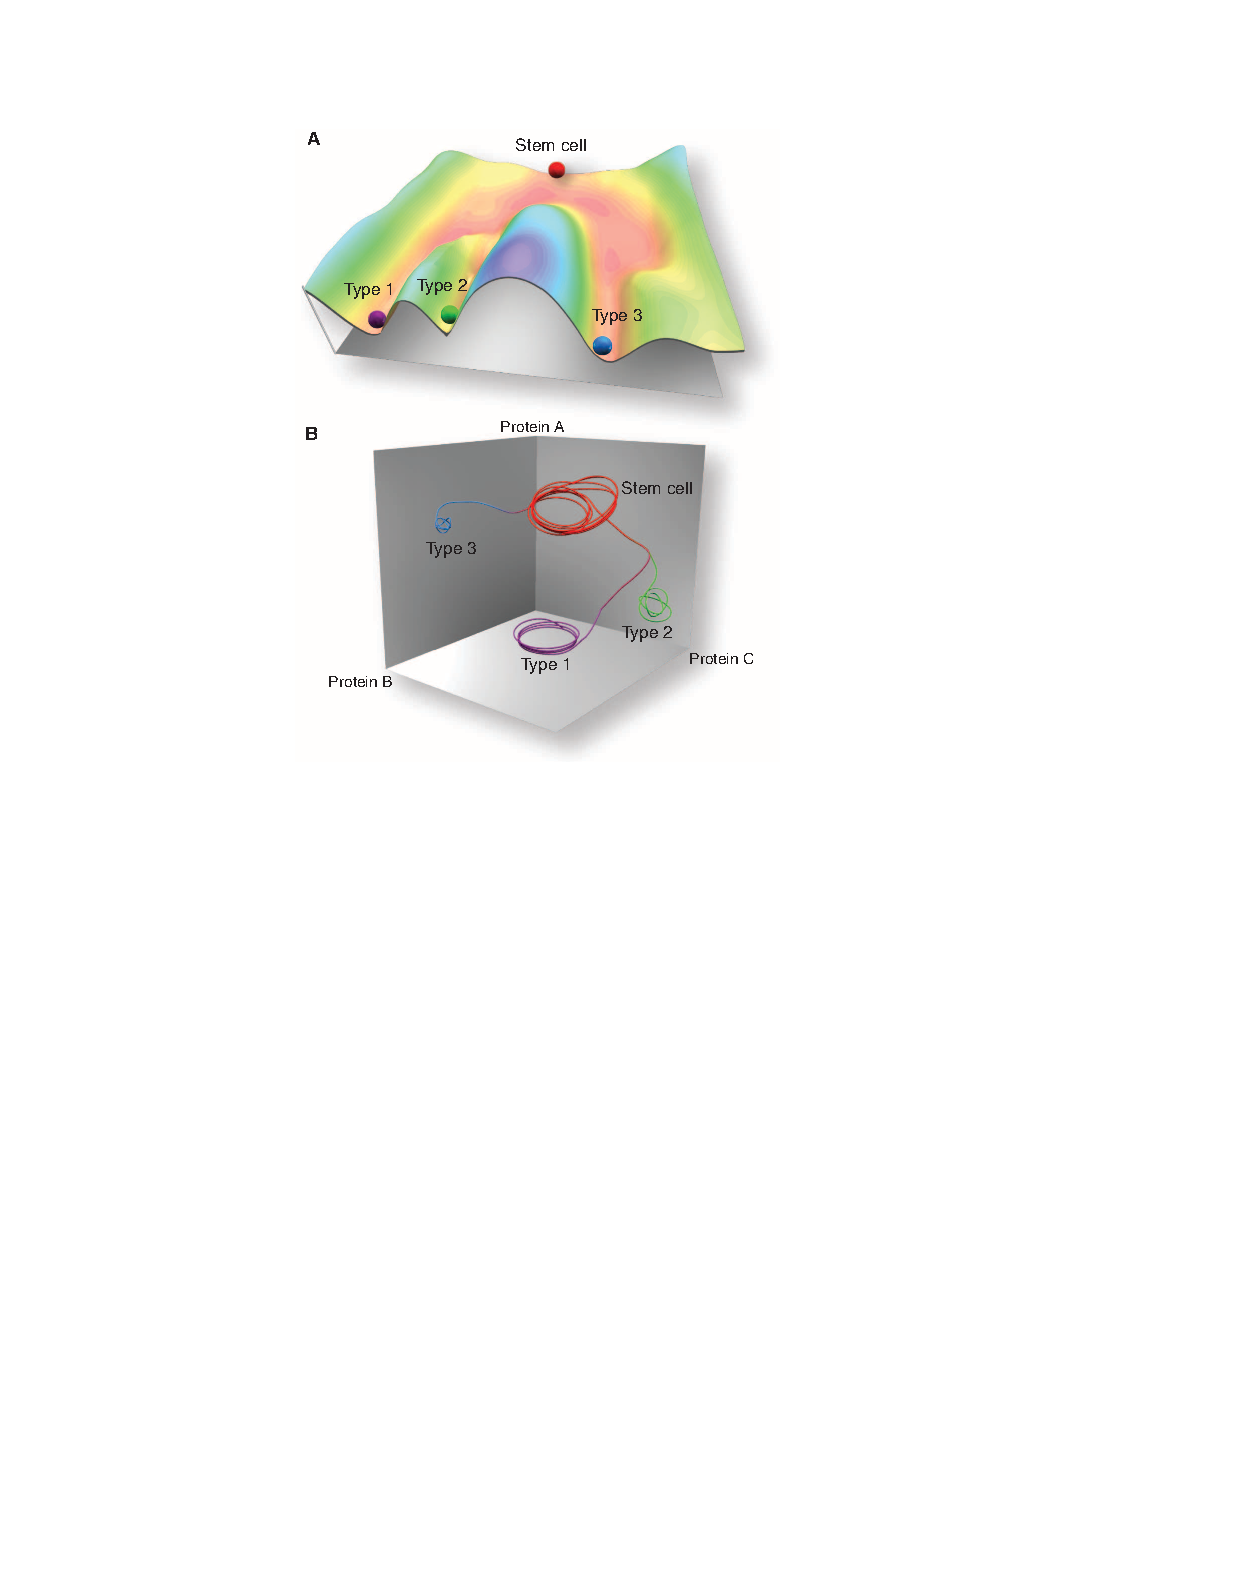
\includegraphics[width=0.5\textwidth]{figures/furusawa-epigenetic-landscape.pdf}
\captionbf{Le paysage de la diff�renciation cellulaire}{ 
    
    Figure tir�e de \cite{Furusawa2012p3898}.  \textbf{A.} Paysage �pig�n�tique
    tel qu'imagin� par Waddington \cite{waddington1957strategy} en r�sonance
    avec la notion de paysage �nerg�tique en physique. Le d�veloppement
    cellulaire est repr�sent� par une bille d�valant un paysage compos� de
    diff�rentes vall�es s�par�es par des barri�res difficilement
    franchissables, repr�sentant les diff�rents types cellulaires et leur
    robustesse face aux fluctuations.  \textbf{B.} Repr�sentation dynamique de
    l'�volution des �tats cellulaires.  Le ph�notype est ici caract�ris� par
    l'expression de trois prot�ines A, B et C, dont l'�volution dans le temps
    peut �tre repr�sent�e par une trajectoire dans un espace tridimensionnel.
    Les �tats souche et diff�renci�s sont caract�ris�s par des bassins
    d'attraction correspondant � diff�rents types cellulaires.  

} 
\label{fig:furusawa-epigenetic-landscape} 
\efig

L'acquisition d'un ph�notype cellulaire particulier au sein d'un organisme est
le sujet de la biologie du d�veloppement. Cette acquisition passe par
diff�rentes �tapes de diff�renciation cellulaire. Sch�matiquement, au cours du
d�veloppement d'un organisme, des cellules non diff�renci�es ou souches
empruntent un chemin unidirectionnel de diff�renciation qui restreint peu � peu
le nombre de types cellulaires qu'elles peuvent potentiellement devenir,
passant de l'�tat souche totipotent � des �tats pluripotents successifs avant
la diff�renciation finale. Ainsi, la formation des cellules somatiques, qui
sont les cellules d'un organisme n'�tant ni souches ni germinales (les cellules
qui donnent naissance aux gam�tes ou cellules sexuelles), est le r�sultat d'un
processus de diff�renciation initial lors du d�veloppement embryonnaire au
cours duquel les cellules issues de l'{\oe}uf donnent naissance � trois
couches de tissus distinctes : l'endoderme (feuillet interne), l'ectoderme
(feuillet externe) et le m�soderme (feuillet interm�diaire). Des
diff�renciations successives ont ensuite lieu au sein de ces couches pour
former divers organes tels que le tube digestif (endoderme), les muscles et les
os (m�soderme), ou encore la peau et le syst�me nerveux (ectoderme).

Dans un �crit aujourd'hui c�l�bre datant de 1957 \cite{waddington1957strategy},
Waddington proposa une repr�sentation de ces diff�rentes �tapes sous la forme
d'un paysage �pig�n�n�tique semblable aux paysages �nerg�tiques dont sont
coutumiers les physiciens (fig~\ref{fig:furusawa-epigenetic-landscape}A).  Dans
cette repr�sentation, le processus de diff�renciation cellulaire est compar�
� une bille d�valant une pente et dont la trajectoire suit les multiples
embranchements de vall�es escarp�es, chacune repr�sentant un �tat de
d�veloppement diff�rent.  Les vall�es sont s�par�es par des pics dont la
hauteur refl�te la difficult� de passer d'un �tat � un autre, et les
destinations finales possibles de la bille correspondent aux diff�rents types
cellulaires.

La notion de trajectoire de diff�renciation peut �tre rendue plus parlante en
adoptant une repr�sentation de syst�me dynamique. Comme nous l'avons vu en
\ref{sub:phenotype}, la cellule contient de nombreux composants : g�nes,
prot�ines ou autres m�tabolites, qui pris dans leur ensemble d�terminent � un
instant donn� l'�tat cellulaire. Il est ainsi possible de repr�senter l'�tat
cellulaire � un temps donn� comme un point dans un espace de grande dimension
dans lequel chaque axe repr�sente l'abondance d'un certain composant
(fig~\ref{fig:furusawa-epigenetic-landscape}B). De par leur r�le primordial
dans la d�finition de l'�tat cellulaire, l'expression des prot�ines (et donc
des g�nes qui les produisent) domine g�n�ralement ces composants, et on parle
de \og niveau d'expression g�n�tique \fg pour d�crire leur abondance. Les
changements d'expression g�n�tique, au cours desquels certains g�nes vont �tre
activ�s et d'autres r�prim�s, induisent un changement de l'�tat cellulaire, ce
qui se traduit par une trajectoire dans l'espace des �tats.  Ces changements
d'expression restreignent finalement l'�tat cellulaire � une certaine r�gion,
d�finie comme un \og attracteur \fg de la dynamique. Une fois au sein d'un
attracteur, l'�tat cellulaire est robuste aux perturbations du niveau
d'expression g�n�tique des diff�rentes composantes. Les attracteurs peuvent
alors �tre vu comme des types cellulaires distincts correspondant aux
diff�rentes vall�es de la repr�sentation de Waddington
\cite{kaufmann1993origins}.


\subsection{La cellule dans l'organisme : une sp�cification spatio-temporelle}

\bfig
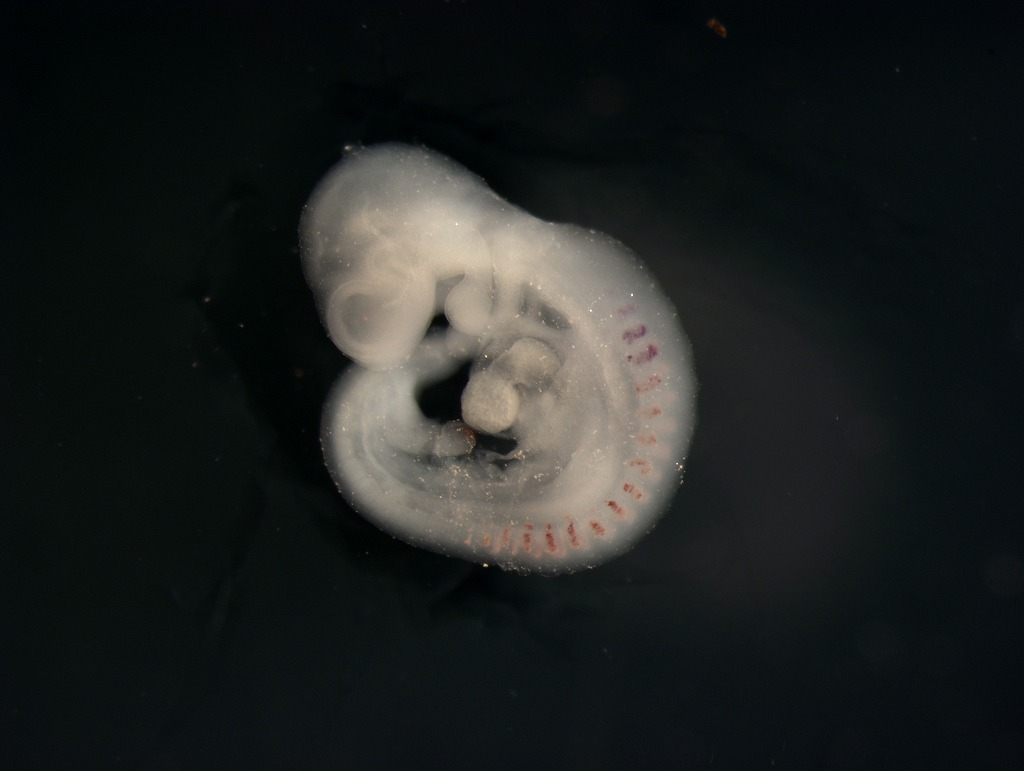
\includegraphics[width=.32\textwidth]{figures/embrys-myog-e9_5.jpg}
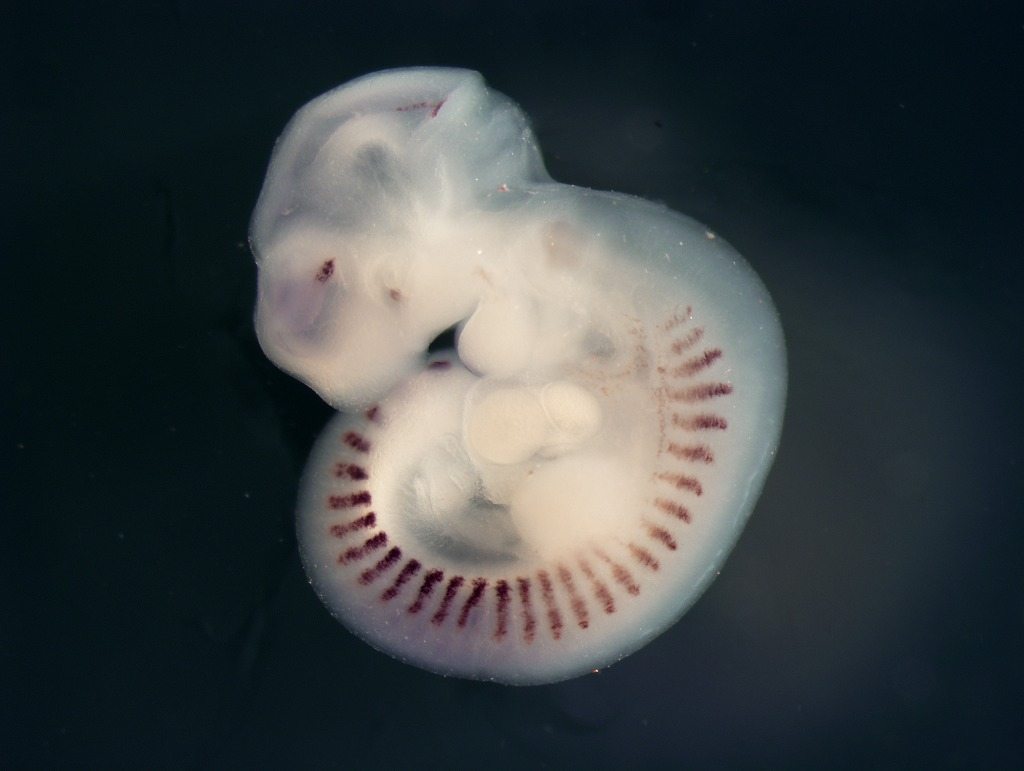
\includegraphics[width=.32\textwidth]{figures/embrys-myog-e10_5.jpg}
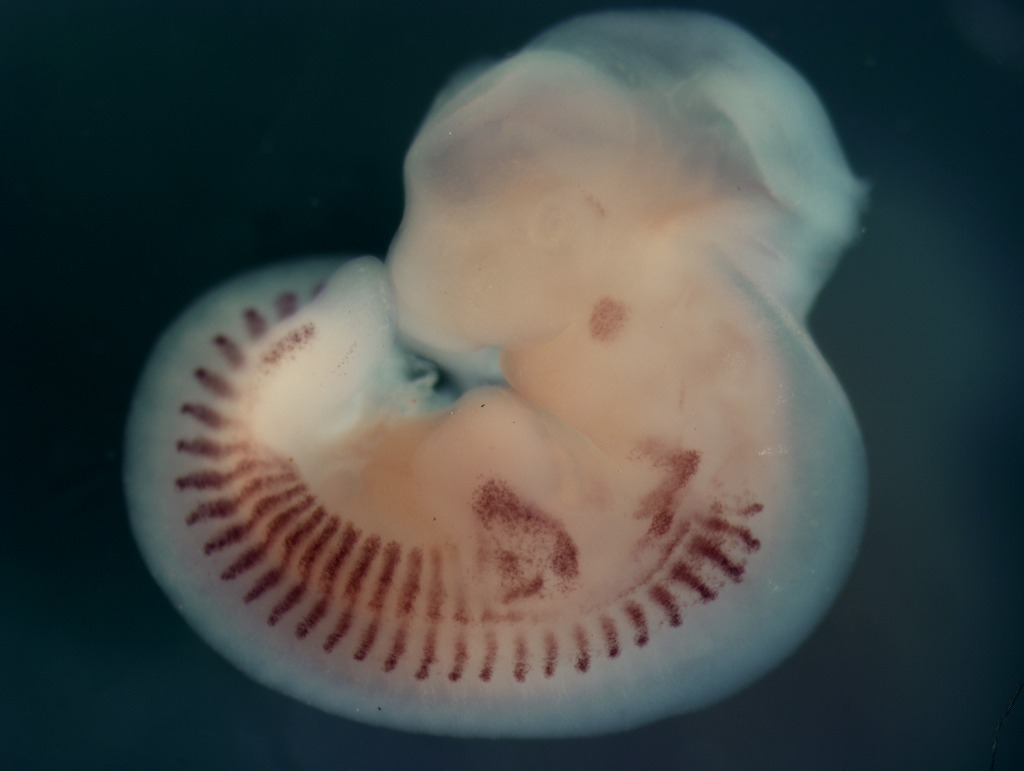
\includegraphics[width=.32\textwidth]{figures/embrys-myog-e11_5.jpg}
\captionbf{Sp�cification spatio-temporelle du type cellulaire}{ 
    
    Hybridation \insitu de l'ARN du g�ne \myog, marqueur de la diff�renciation
    des prog�niteurs du muscle squelettique, chez des embryons de souris �g�s
    de $9.5$, $10.5$ et $11.5$ jours (de gauche � droite), observ�s sous un
    m�me grossissement de $10$. Le motif (\textit{pattern}) de sp�cification du
    muscle squelettique est clairement visible au niveau des somites, lieu des
    futures vert�bres. Images tir�es de la base de donn�e Embrys
    (\url{http://embrys.jp}).

} 
\label{fig:embrys-myog}
\efig

Au sein de l'organisme, la diff�renciation cellulaire op�re � un rythme pr�cis
et dans un contexte environnemental bien d�fini. Aussi, les trajectoires dans
l'espace d'expression g�n�tique que nous avons pr�sent�es pr�c�demment sont
fonction de l'espace -- la position de la cellule dans l'organisme, qui
d�termine en particulier la concentration des signaux qu'elle re�oit de son
environnement -- et du temps -- le stade de d�veloppement de l'organisme --.
Il est ainsi possible d'observer chez l'embryon certains motifs ou
\textit{patterns} spatio-temporels d'expression g�n�tique correspondant � des
organes en formation et r�v�l�s par hybridation \insitu de l'ARN de
certains g�nes sp�cifiques d'un type cellulaire. Par exemple, dans le cas de la
formation des muscles squelettiques, le g�ne de diff�renciation terminale \myog
est exprim� chez la souris d�s $8$ jours embryonnaires au niveau des somites,
segments correspondant aux futures vert�bres de la souris adulte, puis commence
� �tre exprim� au niveau des bourgeons de membres � $11.5$ jours (voir
fig~\ref{fig:embrys-myog}).

 
\subsection{La reprogrammation cellulaire} 
%Fibroblastes, IPS : seulement un ou quelques facteurs suffisent � changer le
%ph�notype d'une cellule.

\bfig
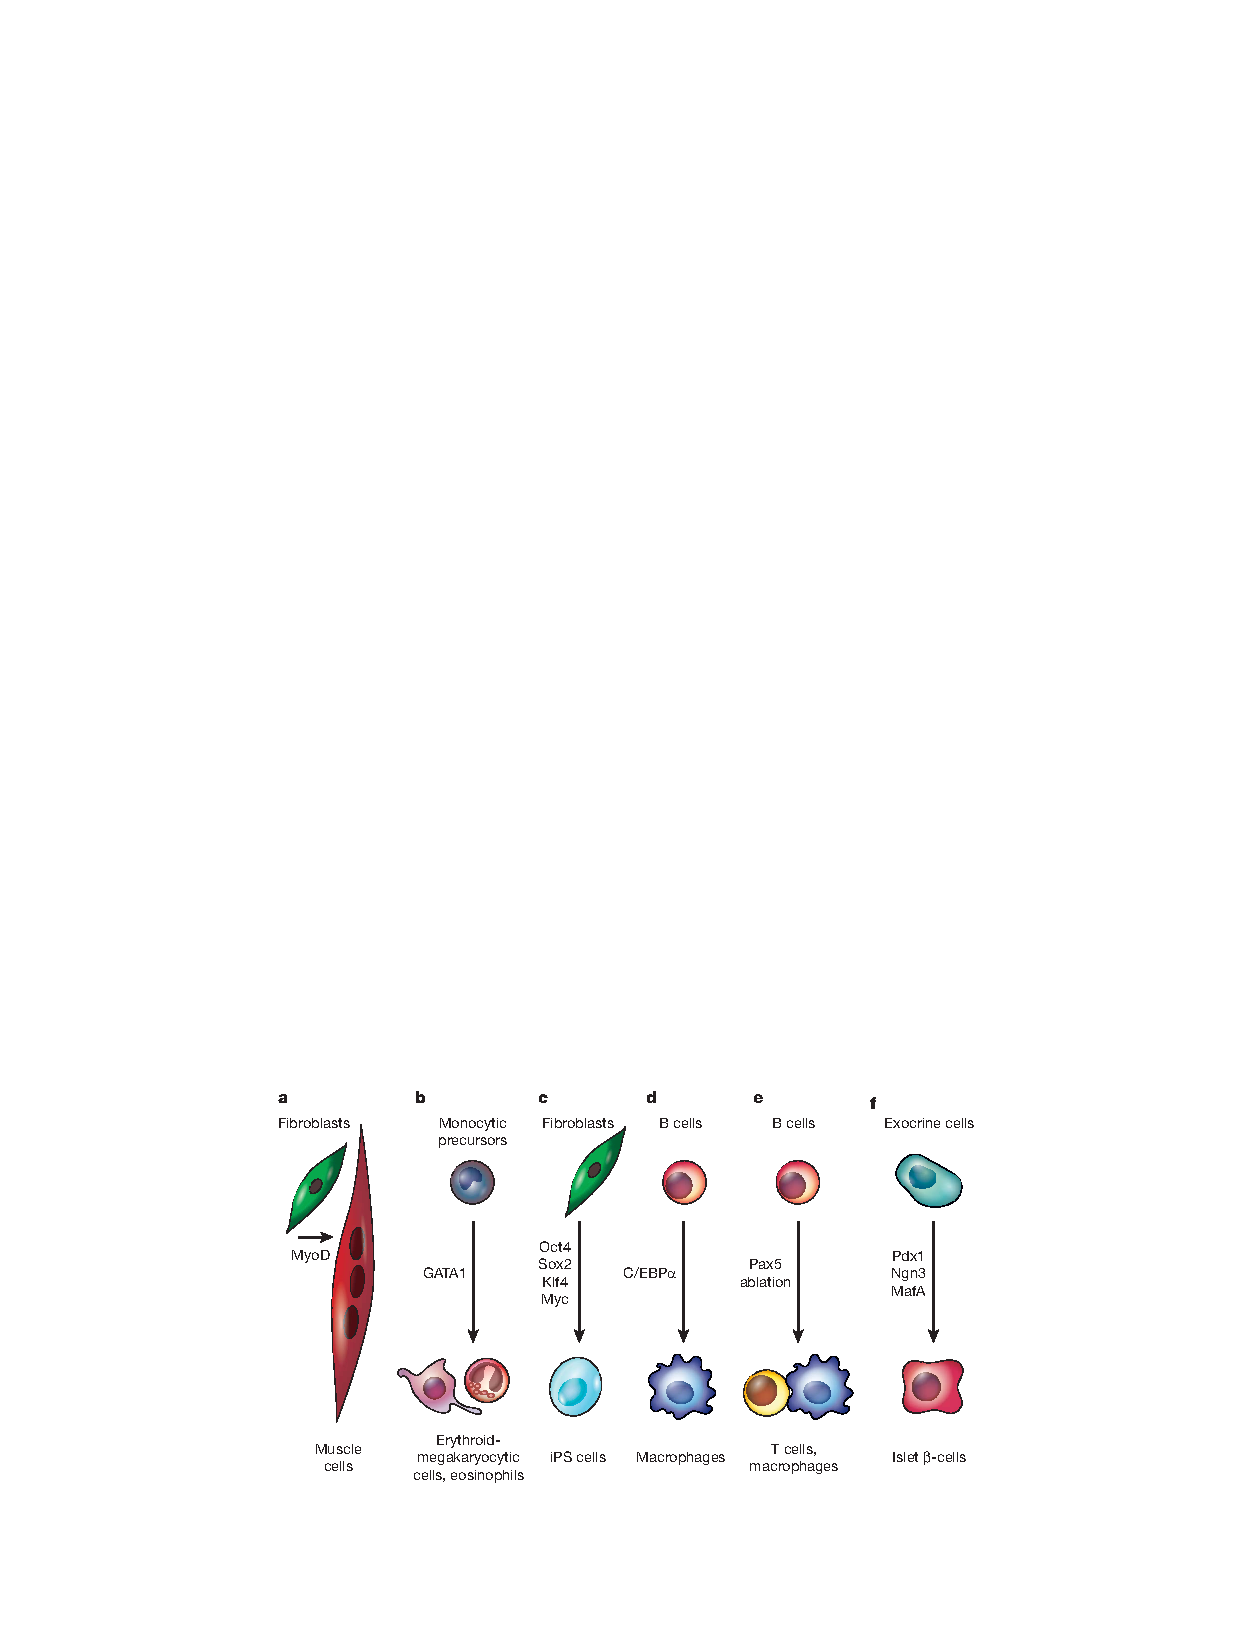
\includegraphics[width=\textwidth]{figures/graf-cells-lineages.pdf}
\captionbf{Diff�rents exemples de reprogrammation cellulaire}{

    Figure tir�e de \cite{Graf2009p2592}, montrant plusieurs exemples
    d'exp�riences de sur-expression ou d'ablation de \fts aboutissant � des
    changements de types cellulaires.  

} 
\label{fig:graf-cells-lineages} 
\efig 

Depuis plusieurs d�cennies, diff�rentes exp�riences ont exhib� la plasticit�
des �tats diff�renci�s, �largissant ainsi consid�rablement la vision classique
selon laquelle des cellules souches totipotentes se diff�rencient de mani�re
irr�versible en des cellules de moins en moins plastiques, jusqu'� atteindre un
�tat diff�renci� stable. Par exemple, \cite{Blau1985vn} ont montr� en $1985$
que des programmes d'expression g�n�tique dormants peuvent �tre exprim�s de
mani�re dominante dans des cellules diff�renci�es par la fusion de diff�rents
types cellulaires : ainsi, la fusion de cellules musculaires avec des cellules
non musculaires permet l'activation des g�nes de type musculaire dans le
type cellulaire non musculaire. Puis diff�rents travaux ont montr� qu'il �tait
possible de convertir des lign�es de cellules diff�renci�es en un autre type
cellulaire en introduisant certaines prot�ines r�gulatrices de la
transcription, ou \FTs (TFs) \cite{davis1987expression,Kulessa1995ys} : on
parle alors de transdiff�renciation, dont l'un des exemples canoniques est la
diff�renciation de cellules de la peau ou fibroblastes en cellules musculaires
par l'introduction du facteur de diff�renciation myog�nique MyoD (voir fig
\ref{fig:graf-cells-lineages}).  Parall�lement, des exp�riences r�alis�es chez
plusieurs esp�ces de mammif�res ont montr� que le transfert de noyaux de
cellules diff�renci�es embryonnaires ou adultes dans un oeuf �nucl�� peut mener
� la formation d'un organisme complet, montrant de mani�re univoque que
l'identit� des cellules diff�renci�es peut �tre compl�tement
renvers�e~\cite{Gurdon2008zr}. Enfin, l'avanc�e la plus r�cente dans ce domaine
a �t� la d�monstration que des cellules somatiques diff�renci�es peuvent �tre
reprogramm�es en cellules souches puripotentes par simple introduction d'un \og
cocktail \fg de 4 \tfs: Oct4, Sox2, c-Myc et Klf4 \cite{Takahashi2006kx} (fig
\ref{fig:graf-cells-lineages}C).



\section{Les r�seaux de r�gulation g�n�tique}

Afin de pouvoir mieux comprendre les m�canismes de diff�renciation et de
reprogrammation expos�s en~\ref{sec:phenotype}, il convient de se plonger dans
les m�canismes internes de la cellule qui r�gissent ses changements d'�tats.

\bfigp
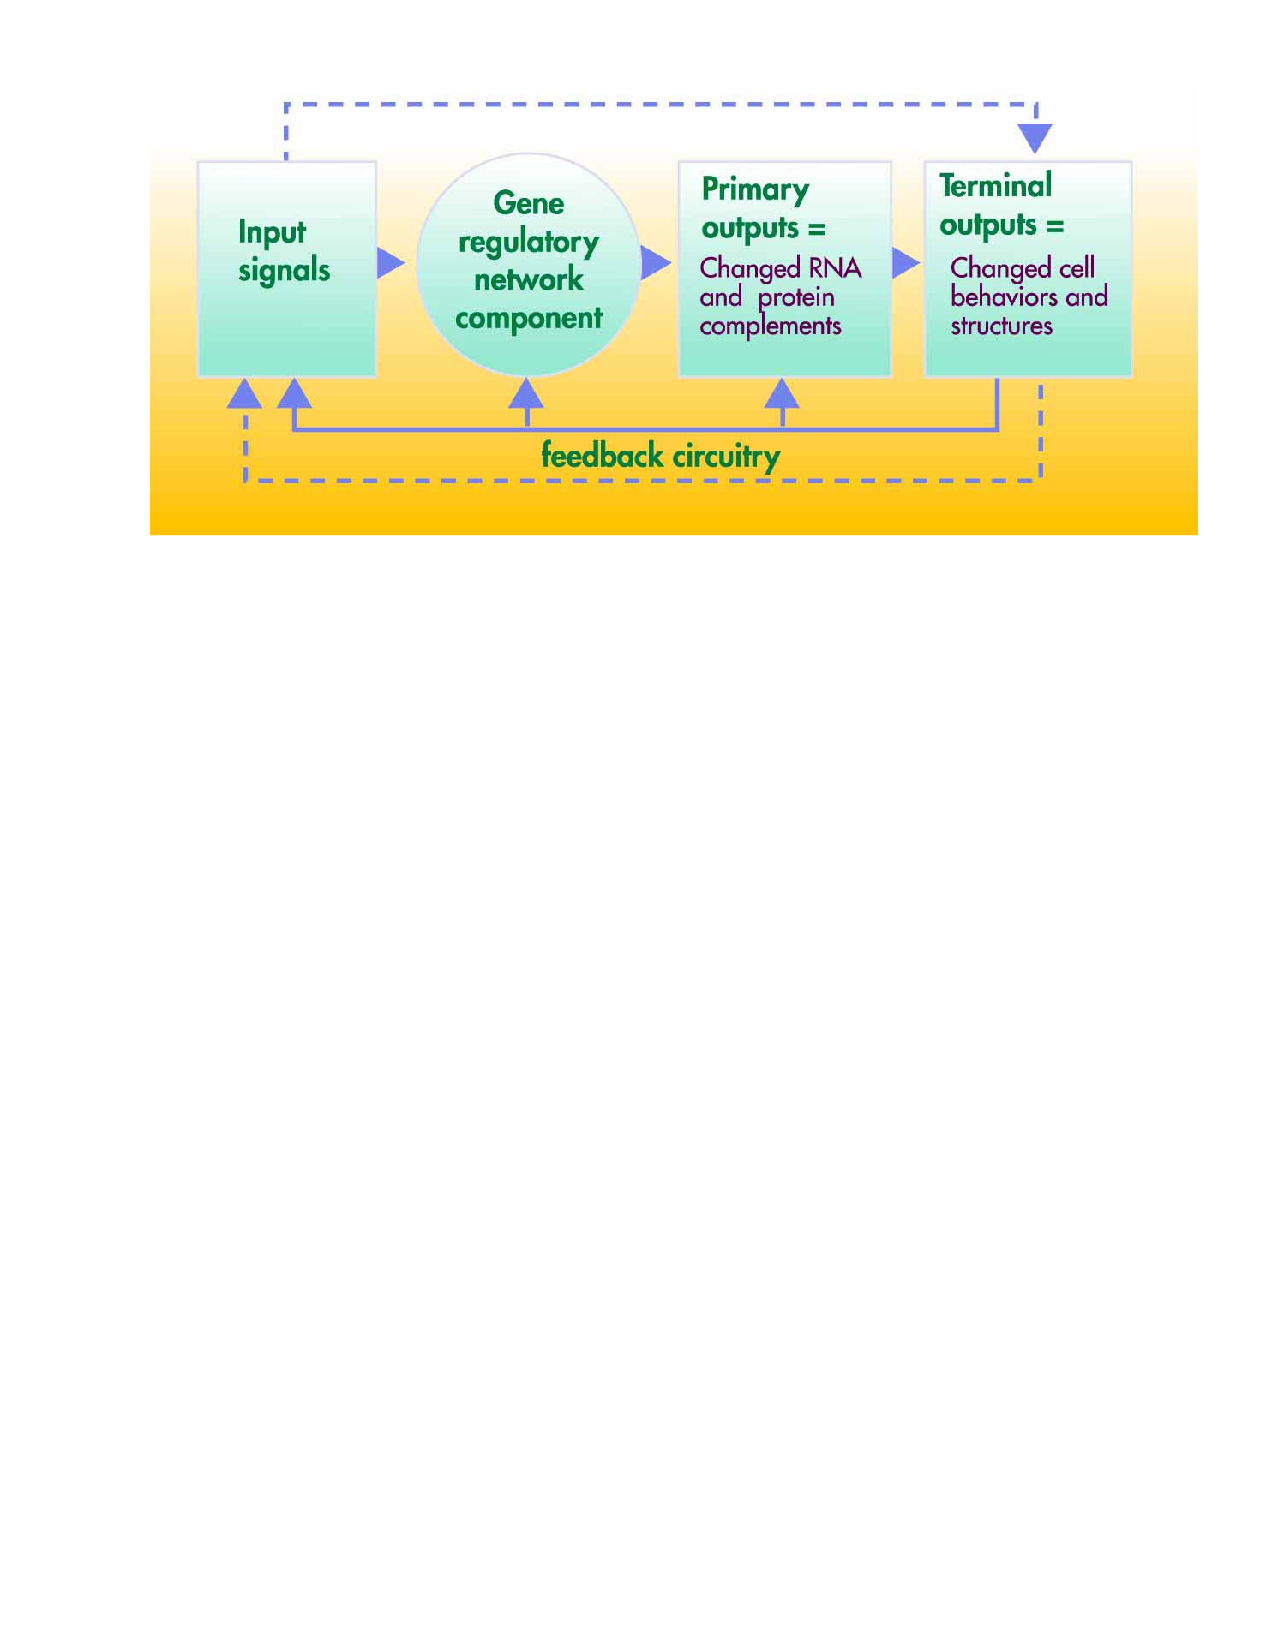
\includegraphics[width=\textwidth]{figures/us-cybernetics.pdf}
\captionbf{Vision cybern�tique du traitement de l'information par la cellule}
{
 
    Figure tir�e du programme `Genomes to life' du D�partement de l'�nergie
    des �tats-Unis datant de 2001 \cite{USDE} sch�matisant un r�seau de
    r�gulation cellulaire comme un syst�me de traitement entr�e/sortie,
    poss�dant trois composantes fondamentales : (1) un syst�me de r�ception et
    de transduction des signaux d'entr�es qui peuvent �tre intra- ou
    extra-cellulaires (plusieurs signaux pouvant affecter un m�me g�ne cible),
    (2) un \og composant central \fg (\textit{core component}) compos� du r�seau de
    r�gulation g�n�tique traitant les signaux, et (3) d'un signal de sortie
    consistant en l'expression mol�culaire des ARNs et prot�ines des g�nes
    cibles. Le processus r�sulte en la modification du ph�notype de la cellule.
    Des boucles de r�gulation (\textit{feedback}) assurent le contr�le et la
    stabilit� des diff�rentes �tapes.

} 
\label{fig:us-cybernetics} 
\efigp


\subsection{Vision cybern�tique de la cellule}

Le paradigme qui r�gne sur la biologie mol�culaire depuis plus d'un demi si�cle
est celui des r�seaux g�n�tiques. L'expression des g�nes est en effet r�gul�e
par des prot�ines, les \fts, qui sont eux-m�mes issus de l'expression d'autres
g�nes, cr�ant ainsi un r�seau d'interactions entre g�nes. Certaines prot�ines
peuvent par ailleurs directement r�guler l'activit� d'autres prot�ines, et
certains ARNs issus de la transcription de g�nes non codants jouent aussi un
r�le fondamental dans la r�gulation de l'activit� g�n�tique, le tout formant un
r�seau complexe d'interactions � diff�rents niveaux. La compr�hension de ce
r�seau et des fonctions qui en r�sultent forme le socle de la biologie des
syst�mes. Dans ce cadre, la cellule est vue comme une unit� de traitement
d'information qui interpr�te diff�rents signaux re�us en entr�e, les traite par
un r�seau interne de r�gulation, et r�agit en sortie en modifiant son �tat ou
son comportement (fig~\ref{fig:us-cybernetics}). L'int�r�t d'une telle
description m�canistique est qu'elle permet d'op�rer quantifications
math�matiques et pr�dictions, ce qui l'a rendue extr�mement fertile au cours
des derni�res d�cennies \cite{Nurse2011p2308}.

\subsection{Divers modes de r�gulation}
\label{sub:divers_modes_de_regulation}

Les modes de r�gulation qui permettent � la cellule d'interpr�ter des signaux
afin de changer d'�tat sont nombreux. Nous allons nous concentrer ici sur ceux
affectant la production d'ARNs ou de prot�ines (fig.~\ref{fig:us-grn}).

\bfigp
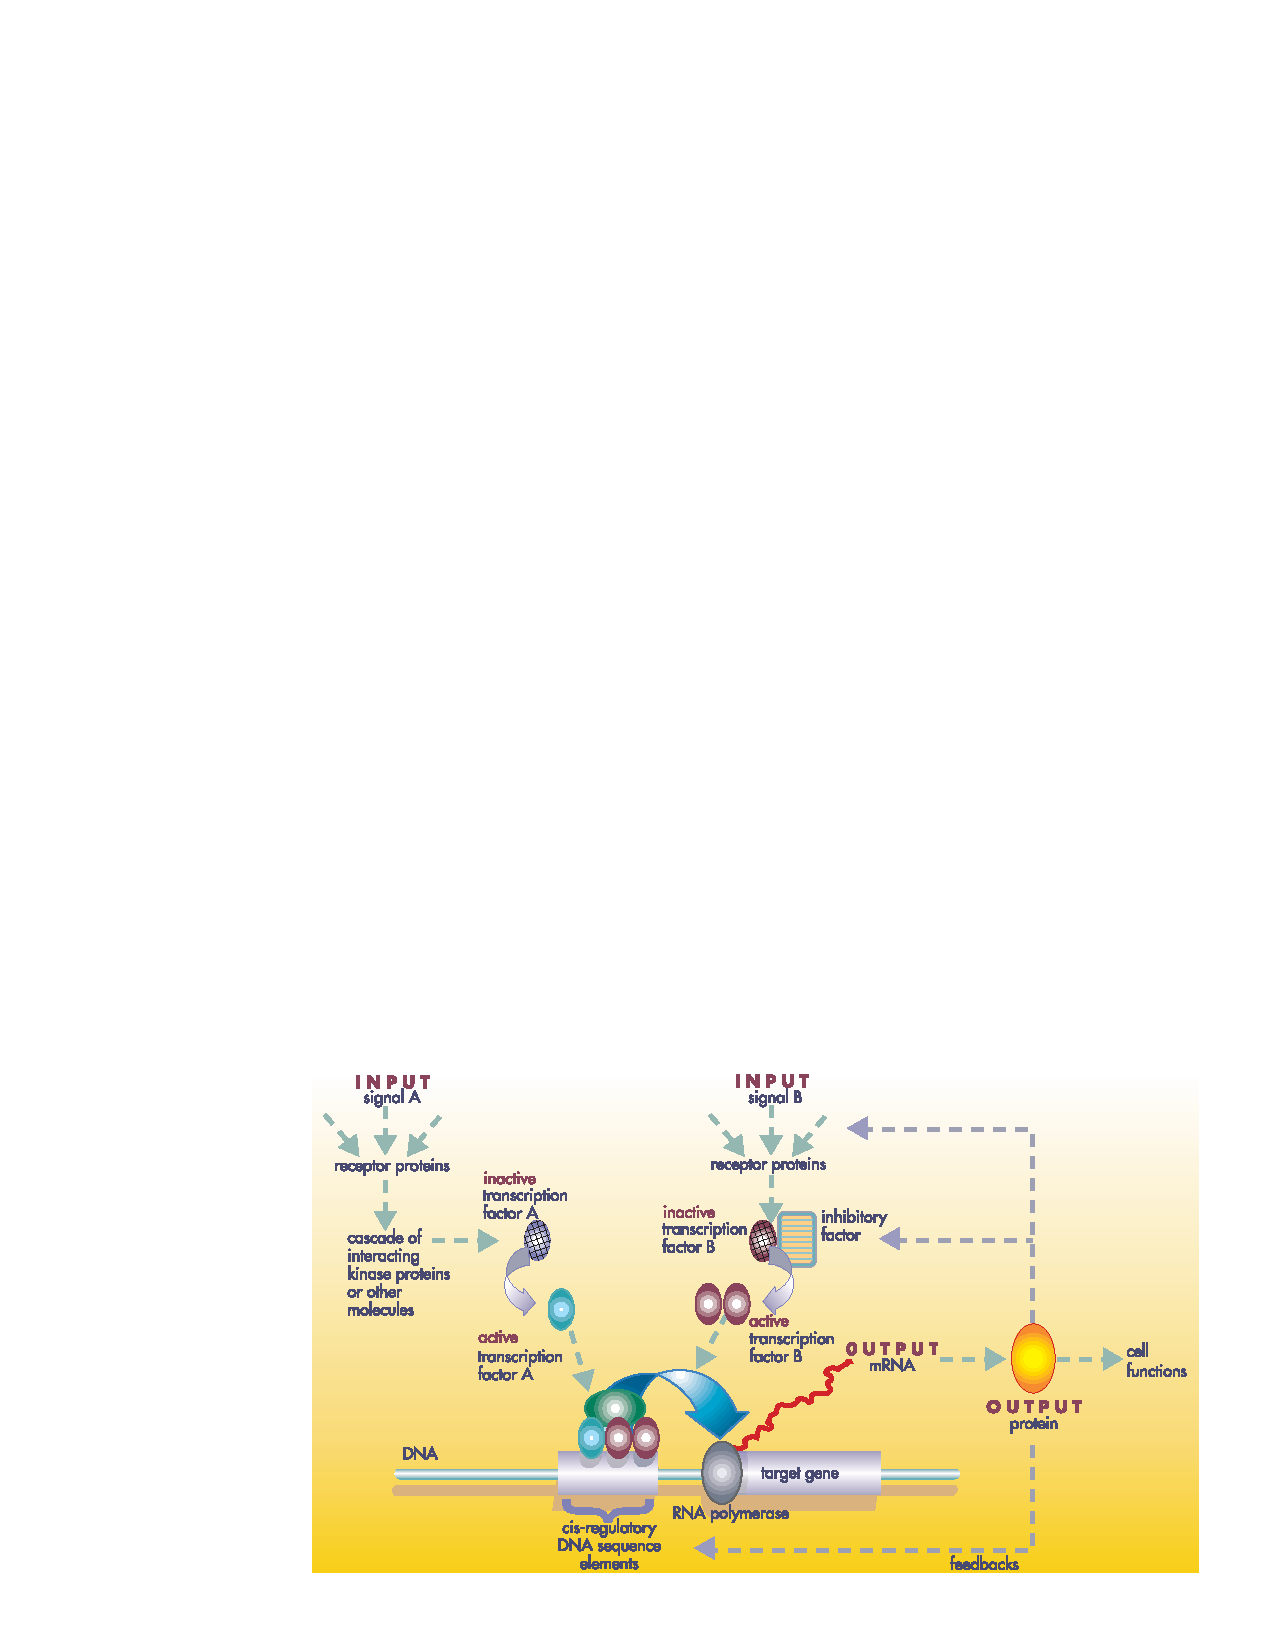
\includegraphics[width=1.0\textwidth]{figures/us-grn.pdf} 
\captionbf{Un r�seau de r�gulation g�n�tique type}{ 
    
    Dans cette repr�sentation sch�matique tir�e du rapport du \citet{USDE},
    deux voies de signalisation A et B transmettent des signaux d'entr�e (qui
    peuvent �tre intra ou extra cellulaires) en rendant des \fts actifs.  Une
    fois activ�s, ces derniers interagissent avec des s�quences d'ADN proches
    d'un g�ne cible en se fixant sur des sites de petite taille ($\sim10$bp).
    Les diff�rents \tfs interagissent entre eux pour former des complexes
    occupant des r�gions de $\sim1000$bp appel�es \crms ou CRMs (voir section
    \ref{sec:CRMs}).  Lorsque les \tfs sont fix�s sur le CRM de leur g�ne
    cible, il peuvent activer ou inhiber la transcription d'ARN et donc la
    production de la prot�ine correspondante.

}    
\label{fig:us-grn} 
\efigp

\subsubsection{R�gulation g�n�tique}

Tout d'abord, un r�seau d'expression g�n�tique est caract�ris� par un jeu
d'interactions entre diff�rents g�nes. Ici, nous centrons notre attention sur
les g�nes codant pour des prot�ines, mais on pourrait inclure les g�nes codant
pour des ARNs non traduits, ceux-ci pouvant �tre impliqu�s dans la r�gulation.
Dans ce r�seau, les interactions se font par l'interm�diaire de prot�ines
r�gulatrices appel�es \fts ou TFs, qui sont au nombre de $\sim1400$ chez
l'homme \cite{Vaquerizas2009ys}, soit $6\%$ des prot�ines encod�es. Les g�nes
qui les expriment repr�sentent donc $\sim3$\% de l'ensemble des $30,000$ g�nes
connus � ce jour. Pour r�guler (activer ou inhiber) la transcription d'un g�ne
cible, les TFs se fixent sur des sites de reconnaissance sp�cifiques sur l'ADN
de $\sim10$bp et interagissent avec la machinerie transcriptionnelle au niveau
du promoteur du g�ne cible. Les TFs peuvent se fixer sur le promoteur m�me,
comme c'est souvent le cas chez la bact�rie, ou dans des r�gions distales
allant jusqu'� plusieurs centaines de kb, comme on trouve plus couramment chez
les organismes complexes. Par ailleurs, diff�rents TFs peuvent se combiner sur
certaines r�gions de r�gulation contenant de multiples sites de fixation pour
former des complexes prot�iques.  Ces r�gions, appel�es \crms (CRMs) ou plus
commun�ment \textit{enhancers}, sont d'une taille typique de $\sim1000$bp et
ont la particularit� de conduire � une expression spatio-temporelle tr�s
sp�cifique du g�ne cible. Ces diff�rents points seront amplement d�velopp�s en
section~\ref{sec:CRMs}.

\bfig
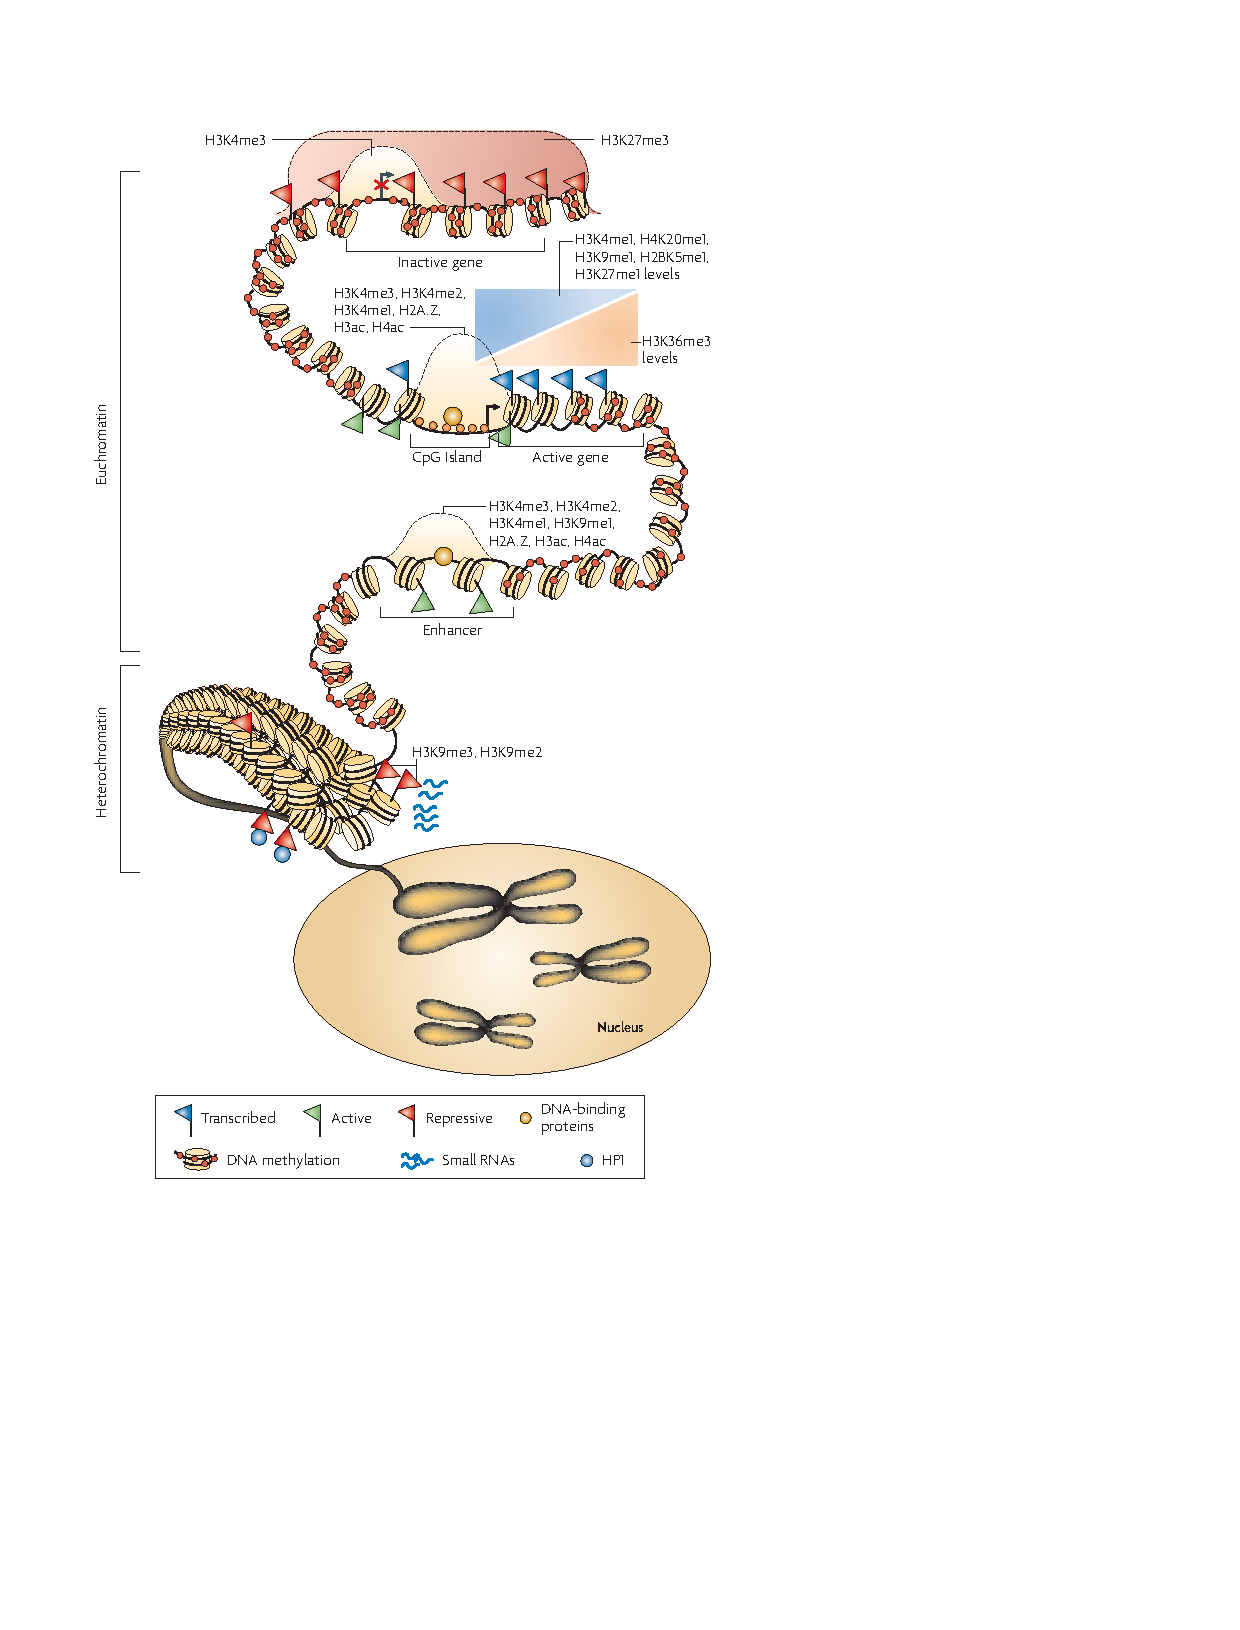
\includegraphics[width=0.7\textwidth]{figures/schones-epigenome.pdf}
\captionbf{Caract�ristiques de l'�pig�nome}{ 
    
    Figure tir�e de~\cite{Schones2008nx}. Les chromosomes sont partag�s entre
    r�gions accessibles d'euchromatine et r�gions difficilement accessibles
    d'h�t�rochromatine. Les r�gions h�t�rochromatiques sont marqu�es par la di-
    et trim�thylation de la lysine 9 de l'histone H3 (H3K9me2 et H3K9me3).  La
    m�thylation de l'ADN est r�pandue � travers tout le g�nome, mais est
    absente de certaines r�gions comme les �lots CpG, les promoteurs et les CRMs.
    La modification H3K27me3 couvre de larges r�gions englobant des g�nes
    inactifs.  Les marques H3K4me3, H3K4me2, H3K4me1 et l'ac�tylation des
    histones marquent les TSSs des g�nes actifs. Les marques H3K4, H3K9, H3K27,
    H4K20 et H2BK5 marquent les r�gions transcrites activement � proximit� de
    la r�gion 5' des g�nes (en amont), alors que la marque H3K36 marque les
    g�nes transcrits dans leur r�gion 3' (en aval). 

} 
\label{fig:schones-epigenome} 
\efig


\subsubsection{R�gulation �pig�n�tique} 


Outre la r�gulation g�n�tique, due � l'action de prot�ines issues de s�quences
codantes et se fixant sur des s�quences d'ADN -- r�gulation qui est donc
enti�rement encod�e dans le g�nome et transmise � la descendance --, il existe
un autre mode de r�gulation de la transcription des g�nes qui permet notamment
d'acqu�rir une modification d'expression g�n�tique transmise � la descendance
sans qu'il y ait modification du code g�n�tique : c'est la r�gulation
�pig�n�tique. Cette r�gulation passe notamment par la modification des
propri�t�s chimiques de l'ADN et des histones sur lequel il s'enroule pour
former la chromatine (fig.~\ref{fig:schones-epigenome})\footnote{Il est � noter
    que certains emploient le terme �pig�n�tique pour qualifier la fixation des
TFs sur l'ADN. Ici, le terme �pig�n�tique r�f�re seulement aux modifications
chimiques affectant les histones et l'ADN, et donc l'accessibilit� du g�nome}.
Ainsi, la m�thylation des dim�res CpG de l'ADN\footnote{Les dim�res C-G sont
appel�s CpG, o� p caract�rise le phosphore liant les deux bases, pour les
diff�rencier du CG utilis� pour parler de la statistique en C et G de l'ADN} au
niveau des r�gions riches en CG, ou �lots CpG, situ�es pr�s de nombreux
promoteurs et habituellement d�pourvues de ces marques conduit � une
inactivation du g�ne cible~\cite{Bird2002oq}.  Par ailleurs, la m�thylation des
histones au niveau des r�sidus lysines entra�ne la fermeture de la chromatine,
emp�chant l'expression du ou des g�ne(s) situ�s � leur niveau, alors que
l'ac�tylation des m�mes lysines entra�ne au contraire une ouverture de la
chromatine, favorisant ainsi la transcription g�n�tique~\cite{Greer2012ve}.  Ce
mode de r�gulation sera d�velopp� plus en d�tail en
section~\ref{sub:les_diff_rents_types_de_crms}.

% lincRNAs? \cite{Rinn2012p3940}

\subsubsection{R�gulation post-transcriptionnelle} 

Les modifications post-transcriptionnelles affectent les ARNs issus de la
transcription des g�nes. Ces modifications peuvent �tre caus�es par des
microARNs ou miRNAs qui sont des ARNs de $\sim23$ nts issus d'ARNs se repliant
en structure double brin de type \og �pingles � cheveux \fg ou
\textit{hairpins}. Les miRNAs s'associent � la prot�ine \textit{Argonaute} du
complexe RISC (\textit{RNA-induced silencing complex}) pour entra�ner la
d�gradation sp�cifique d'ARNms~\cite{Bartel2009cr}. De mani�re similaire,
certains \textit{hairpins} de taille plus importante sont cliv�s par la
prot�ine Dicer pour former plusieurs petits ARNs de taille similaire aux
miRNAs: ce sont les siRNAs (\textit{small interfering RNAs)}). Ceux-ci
recrutent aussi le complexe prot�ique RISC et ciblent sp�cifiquement des
ARNm~\cite{Hammond2001bh,Hannon2002qf}. Ce ph�nom�ne est connu sous le nom
d'interf�rence ARN (RNAi) et a donn� lieu � une m�thode aujourd'hui couramment
utilis�e pour inhiber l'expression d'un g�ne.


\subsubsection{R�gulation post-traductionnelle}

Les modifications post-traductionnelles affectent les prot�ines issues de la
traduction des ARNs. Elles passent par une modification chimique
des prot�ines, typiquement la phosphorylation, ou comme nous l'avons vu pour la
r�gulation �pig�n�tique, la m�thylation ou l'ac�tylation. Ces modifications
peuvent avoir pour effet de changer l'activit� de la prot�ine, que ce soit en
modifiant son activit� enzymatique ou en d�clenchant sa relocalisation
nucl�aire. Il existe aussi des modifications de structure de la
prot�ine, comme c'est le cas du \tf \textit{Shavenbaby} chez la Drosophile:
dans sa forme native, cette prot�ine inhibe la transcription de ses g�nes cible
; cependant ses r�sidus terminaux peuvent �tre cliv�s par des petits peptides
de 11 � 32 acides amin�s encod�s par le g�ne \textit{Pri}, rendant la prot�ine
transcriptionnellement active \cite{Kondo2010ly}.


\bfig
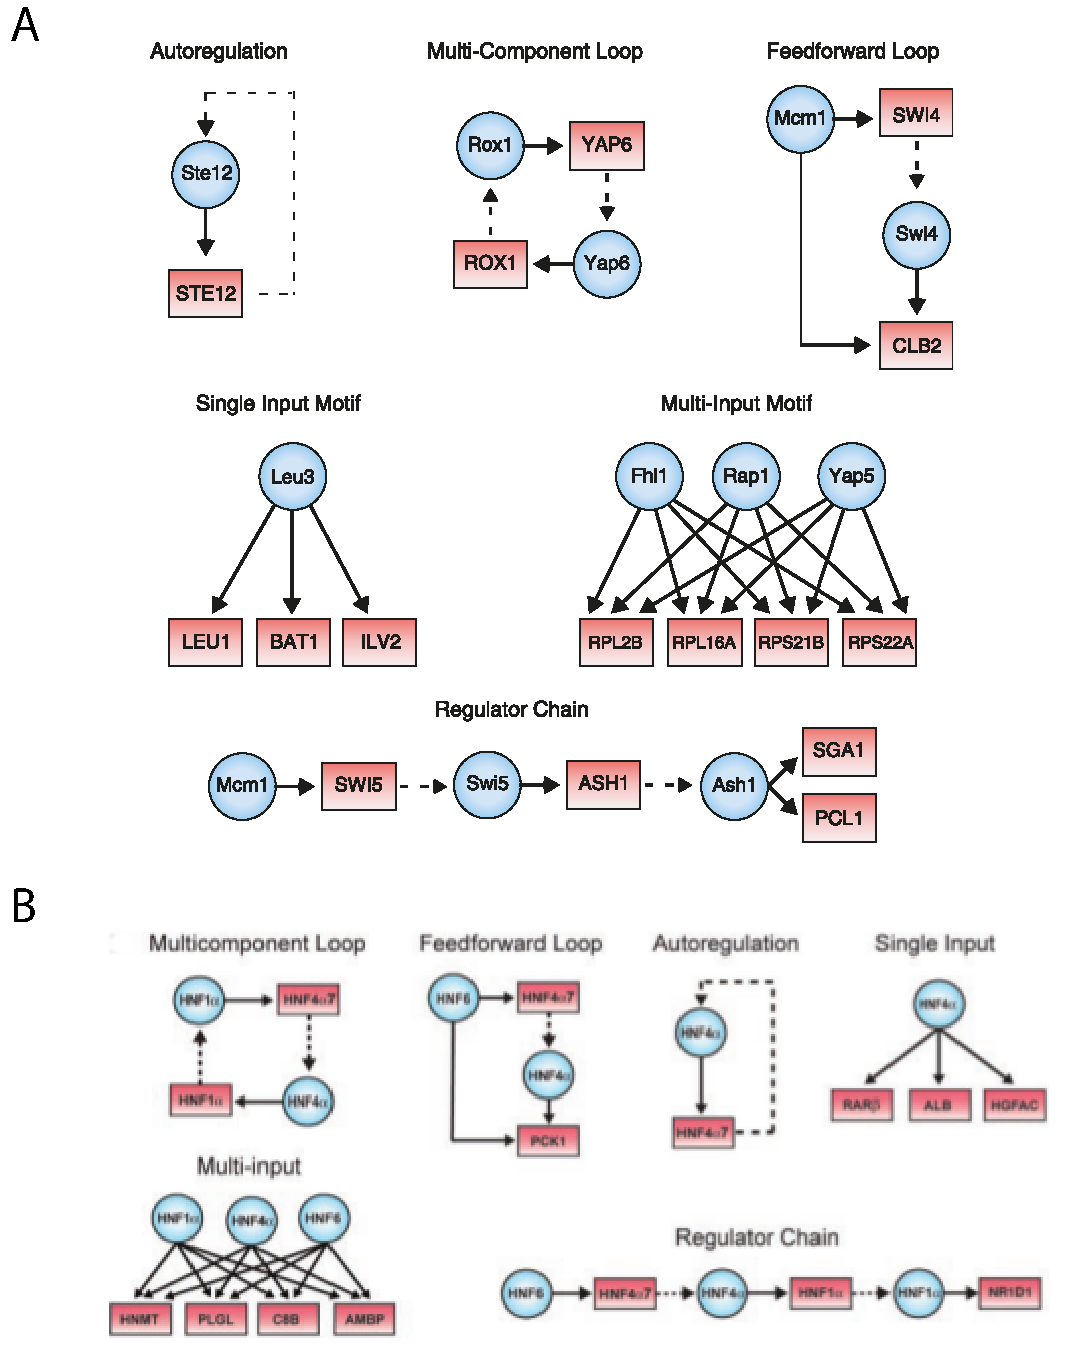
\includegraphics[width=1\textwidth]{figures/lee-network-motifs-yeast.pdf}
\captionbf{Exemples de motifs dans les r�seaux de r�gulation g�n�tique}{
    
    Ces exemples sont issus d'analyses d'interactions entre \tfs (cercles
    bleus) et promoteurs (rectangles rouges) (A) chez la
    levure~\cite{Lee2002p537} et (B) chez l'homme~\cite{Odom2004hc}.  Les
    fl�ches solides indiquent la fixation d'un \tf � un promoteur, et les
    fl�ches en pointill� indiquent l'expression d'un \tf � partir de son g�ne.

}
\label{fig:lee-odom-networks}
\efig

\FloatBarrier
\subsection{C�blage du r�seau et fonction}

Maintenant que nous avons vu la nature des interactions au sein des r�seaux
g�n�tiques, nous pouvons nous pencher sur leur structure. Notamment, plusieurs
�tudes r�alis�es chez divers organismes de la bact�rie � l'homme ont r�v�l� que
les r�seaux de transcription contiennent un petit ensemble de motifs de
r�gulation r�currents, appel�s motifs de
r�seaux~\cite{alon2007introduction,ShenOrr2002p648,Milo2002tg}
(fig.~\ref{fig:lee-odom-networks}).  
%Ces motifs peuvent �tre vus comme les pi�ces �l�mentaires servant � la
%construction de r�seaux fonctionnels. 
De tels motifs furent d'abord d�tect�s de mani�re syst�matique chez la bact�rie
\ecoli en remarquant qu'ils apparaissaient dans le r�seau de transcription bien
plus souvent qu'on ne l'attendrait dans un r�seau
al�atoire~\cite{ShenOrr2002p648}.  Les m�mes motifs ont ensuite �t� trouv�s
chez la levure~\cite{Milo2002tg,Lee2002p537} et chez l'homme~\cite{Odom2004hc}.
Une explication possible de la r�currence de ces motifs est li�e aux fonctions
qu'ils remplissent. Par exemple, la boucle d'autor�gulation n�gative, qui est
trouv�e chez la moiti� des r�presseurs d'\ecoli, poss�de deux fonctions : l'une
est de parvenir rapidement � un �tat d'�quilibre en utilisant un promoteur
fort, l'autre est de servir de tampon au bruit
d'expression~\cite{Alon2007p2353}. Un autre motif r�current est la boucle
feedforward. Celle-ci consiste en 3 g�nes : un r�gulateur X, qui r�gule Y, tous
deux r�gulant Z. Dans le cas o� des interactions sont des activations et que
X et Y sont requis pour activer Z, cette boucle peut servir de tampon au bruit
d'expression de X, �vitant que des fluctuations de son niveau d'expression
n'entra�ne par erreur l'activation de Z.


\FloatBarrier
\subsection{�volution des r�seaux g�n�tiques}

\bfig
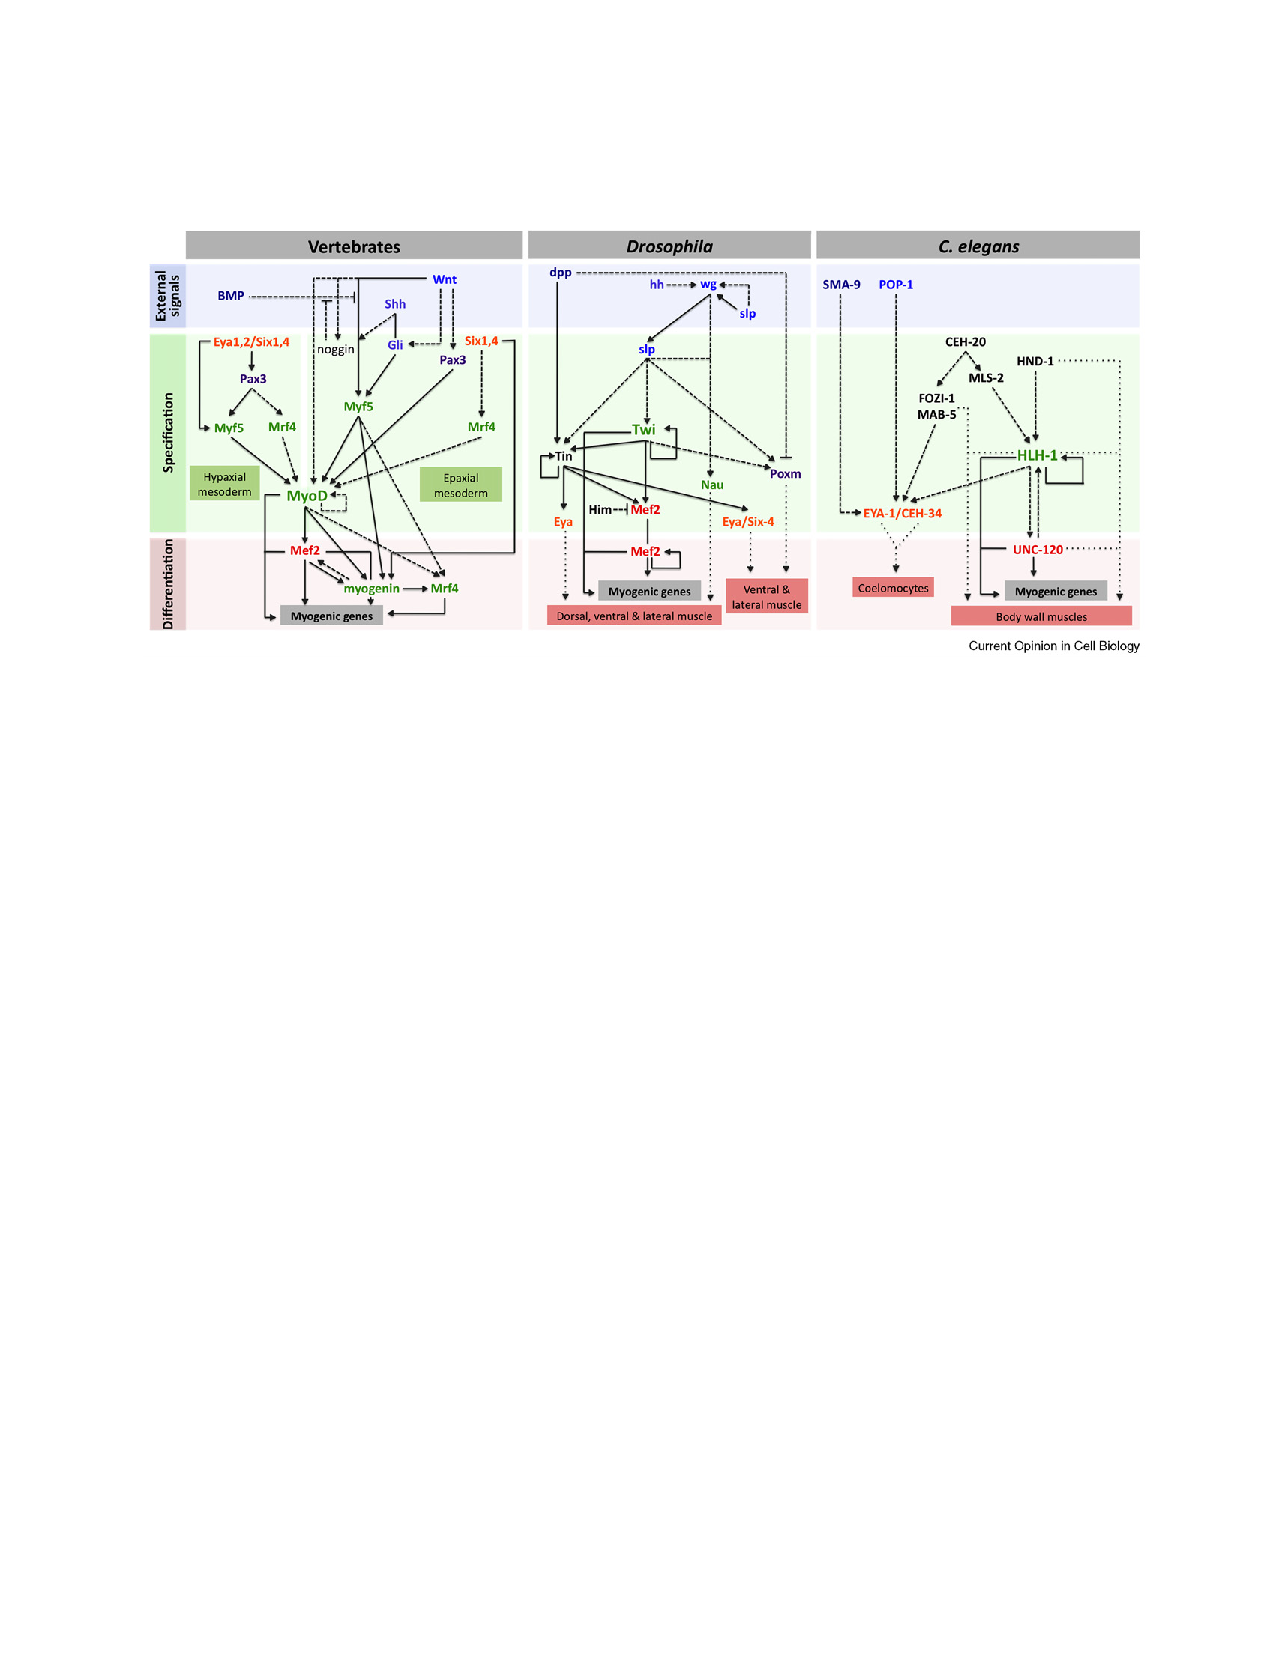
\includegraphics[width=\textwidth]{figures/furlong-network-evolution.pdf}
\captionbf{�volution du r�seau transcriptionnel : l'exemple de la r�gulation
myog�nique.}{ Figure tir�e de \cite{Liu2009p556}. Les lignes pleines indiquent
une r�gulation transcriptionnelle directe, les tirets indiquent des
interactions g�n�tiques dont le caract�re direct n'a pas �t� montr�, et les
lignes pointill�s indiquent que l'interaction est sugg�r�e par des donn�s
d'expression. \myod est l'analogue structurel de \textit{Nautilus} mais est
l'analogue fonctionnel de \textit{Twist} chez la Drosophile et de
\textit{HLH-1} chez \celeg. Les couleurs indiquent respectivement des voies
de signalisation externes au m�soderme (bleu), les r�gulateurs myog�niques de
la famille bHLH (vert), les prot�ines Six/Eya (orange), les prot�ines de la
famille \textit{paired-box} Pax (violet), les TFs des familles MADS/SRF
(rouge), et les r�gulateurs d'autres familles de prot�ines (noir).}
\label{fig:furlong-network-evolution}\efig

L'importance des motifs est rendue plus claire lorsque l'on
s'int�resse � l'�volution des r�seaux. En effet, au cours de l'�volution, les
r�seaux de r�gulation g�n�tique changent : modification des constituants,
rec�blage du r�seau, duplication d'�l�ments\ldots N�anmoins, certaines
modifications sont plus d�favoris�es du point de vue �volutif que des autres.
Ainsi, les motifs tels que les boucles d'autor�gulation ou les boucles
feedforward, de par leur importance fonctionnelle, auront tendance � �tre
conserv�s.  Pour ce qui est des �l�ments du r�seau, la modification d'un
r�gulateur, par exemple la mutation d'un acide amin� au sein d'un \tf, aura des
cons�quences sur l'ensemble des �l�ments r�gul�s par ce \tf et pourra donc �tre
fortement d�l�t�re. Par contre, la modification d'un site de reconnaissance de
ce \tf sur l'ADN n'aura qu'une port�e locale sur la r�gulation du g�ne associ�.
\\ 

� titre d'exemple, prenons le cas du r�seau de diff�renciation du muscle
squelettique pr�sent� en figure~\ref{fig:furlong-network-evolution}, que nous
�tudierons plus en d�tail dans le chapitre \ref{chap:muscle} de ce manuscrit.
Au coeur de ce r�seau g�n�tique se trouvent les facteurs de r�gulation
myog�niques ou MRFs, des \fts de type bHLH qui ont la capacit� de convertir des
cellules non mesodermales, \cad n'�tant pas destin�es � devenir des
prog�niteurs musculaires, en cellules ayant des propri�t�s
musculaires~\cite{Weintraub1989ij}. Ces facteurs sont dits \og r�gulateurs
ma�tres \fg de la diff�renciation musculaire. Chez les vert�br�s il y a quatre
MRFs: \myf, \mrf, \myod, qui ont des roles redondant dans la sp�cification des
prog�niteurs musculaires, et \myog, qui conduit � la diff�renciation terminale.
Chez la \droso c'est le TF  \twi qui semble �tre le principal MRF, mais
contrairement aux MRFs des vert�br�s, son r�le ne s'arr�te pas au contr�le de
la diff�renciation musculaire mais est plus g�n�ral dans le d�veloppement du
m�soderme~\cite{Baylies1998bs}. C'est cependant le g�ne \textit{Nautilus} qui
poss�de la s�quence d'acides amin�s la plus proche de celle des MRFs vert�br�s.
Ce dernier permet la sp�cification des prog�niteurs myog�niques, et son
expression est restreinte au d�veloppement musculaire.  N�anmoins, les mutants
\textit{nautilus} sont viables et son r�le semble mineur compar� aux MRFs
vert�br�s. Enfin, chez le ver \celegans, c'est l'orthologue de \myod,
\textit{hlh-1}, qui tient r�le de MRF.\\ 

Malgr� ces diff�rences (nombre
de MRFs, membre de la famille bHLH tenant ce r�le), on retrouve dans les trois
cas une boucle feedforward conserv�e au niveau de la r�gulation des cibles des
MRFs (fig.~\ref{fig:furlong-network-evolution}).  Ainsi, MyoD r�gule
l'expression de Mef2 et l'activit� de MAPK p38 en m�me temps que l'expression
de plusieurs cibles initiales, et par la suite MyoD et phospho-Mef2 co-r�gulent
des g�nes plus tardifs. Ce m�canisme permet ainsi de r�guler l'aspect temporel
de l'expression g�n�tique.  Chez la Drosophile, le m�me motif est observ� avec
Twist et Mef2 et chez \celeg avec HLH-1 et le TF UNC-129, de la m�me
famille que Mef2.  \\ 

Le coeur du r�seau est donc conserv� dans la forme
(topologie), m�me s'il y a des divergences dans le fond (membres de la famille
de TFs impliqu�s). N�anmoins, les �l�ments r�gulateurs en amont, ainsi que les
membres p�riph�riques du r�seau ont rapidement �volu�. Par exemple, chez les
vert�br�s le TF Pax3 est tr�s en amont dans la hi�rarchie g�n�tique et permet
l'activation des MRFs et la sp�cification myog�nique, alors que chez la
Drosophile son homologue \textit{poxm} est en aval des MRFs et sa perte de
fonction n'a que des effets mineurs sur la myogen�se. Par ailleurs, le complexe
compos� de prot�ine Six et de leur cofacteur Eya, initialement d�couvert comme
r�gulateur majeur de la diff�renciation oculaire chez la \droso, est chez les
vert�br�s un r�gulateur essentiel situ�s en amont des MRFs. Chez la Drosophile,
il poss�de aussi un r�le dans la sp�cification myog�nique, mais bien plus en
aval que chez les vert�br�s. Enfin, chez \celeg ce complexe est aussi en
aval des MRFs mais il participe en plus � la d�termination de cellules non
myog�niques.  \\

Nous voyons donc que l'�volution d'un r�seau g�n�tique poss�de de multiples
facettes : conservation de motifs de r�seau fonctionnellement importants (dans
notre exemple, la boucle feedforward au coeur du r�seau r�gissant l'aspect
temporel de l'expression des cibles), rec�blage des interactions pour traiter
diff�rents signaux d'entr�e\ldots Par ailleurs, il appara�t que plus qu'� des
TFs particuliers, c'est � des familles de TFs que nous avons affaire. Aussi un
m�me r�le au sein du r�seau peut-il �tre rempli par diff�rents membres d'une
m�me famille, comme c'est le cas pour \myod et \twi. Ceci s'explique par le
fait que les membres d'une m�me famille partagent des propri�t�s d'interaction
avec l'ADN semblables. Ces interactions sont � la source du fonctionnement du
r�seau, et nous allons maintenant pr�senter plus en avant leurs propri�t�s.




\FloatBarrier
\section{Les interactions prot�ine-ADN : mod�les math�matiques}

Nous l'avons vu, les interactions entre \tfs et ADN sont une composante
essentielle des r�seaux g�n�tiques. Les TFs se fixent sur des sites sp�cifiques
de $\sim10$ bp dans le voisinage des g�nes qu'ils r�gulent. Trouver ces sites
est donc un premier pas vers la reconstruction des r�seaux de r�gulation
sous-jacents. Dans cette section nous pr�sentons les mod�les d'interactions
prot�ine-ADN qui ont �t� propos�s, et leur application concr�te � la recherche
de sites de fixation. 

\bfig
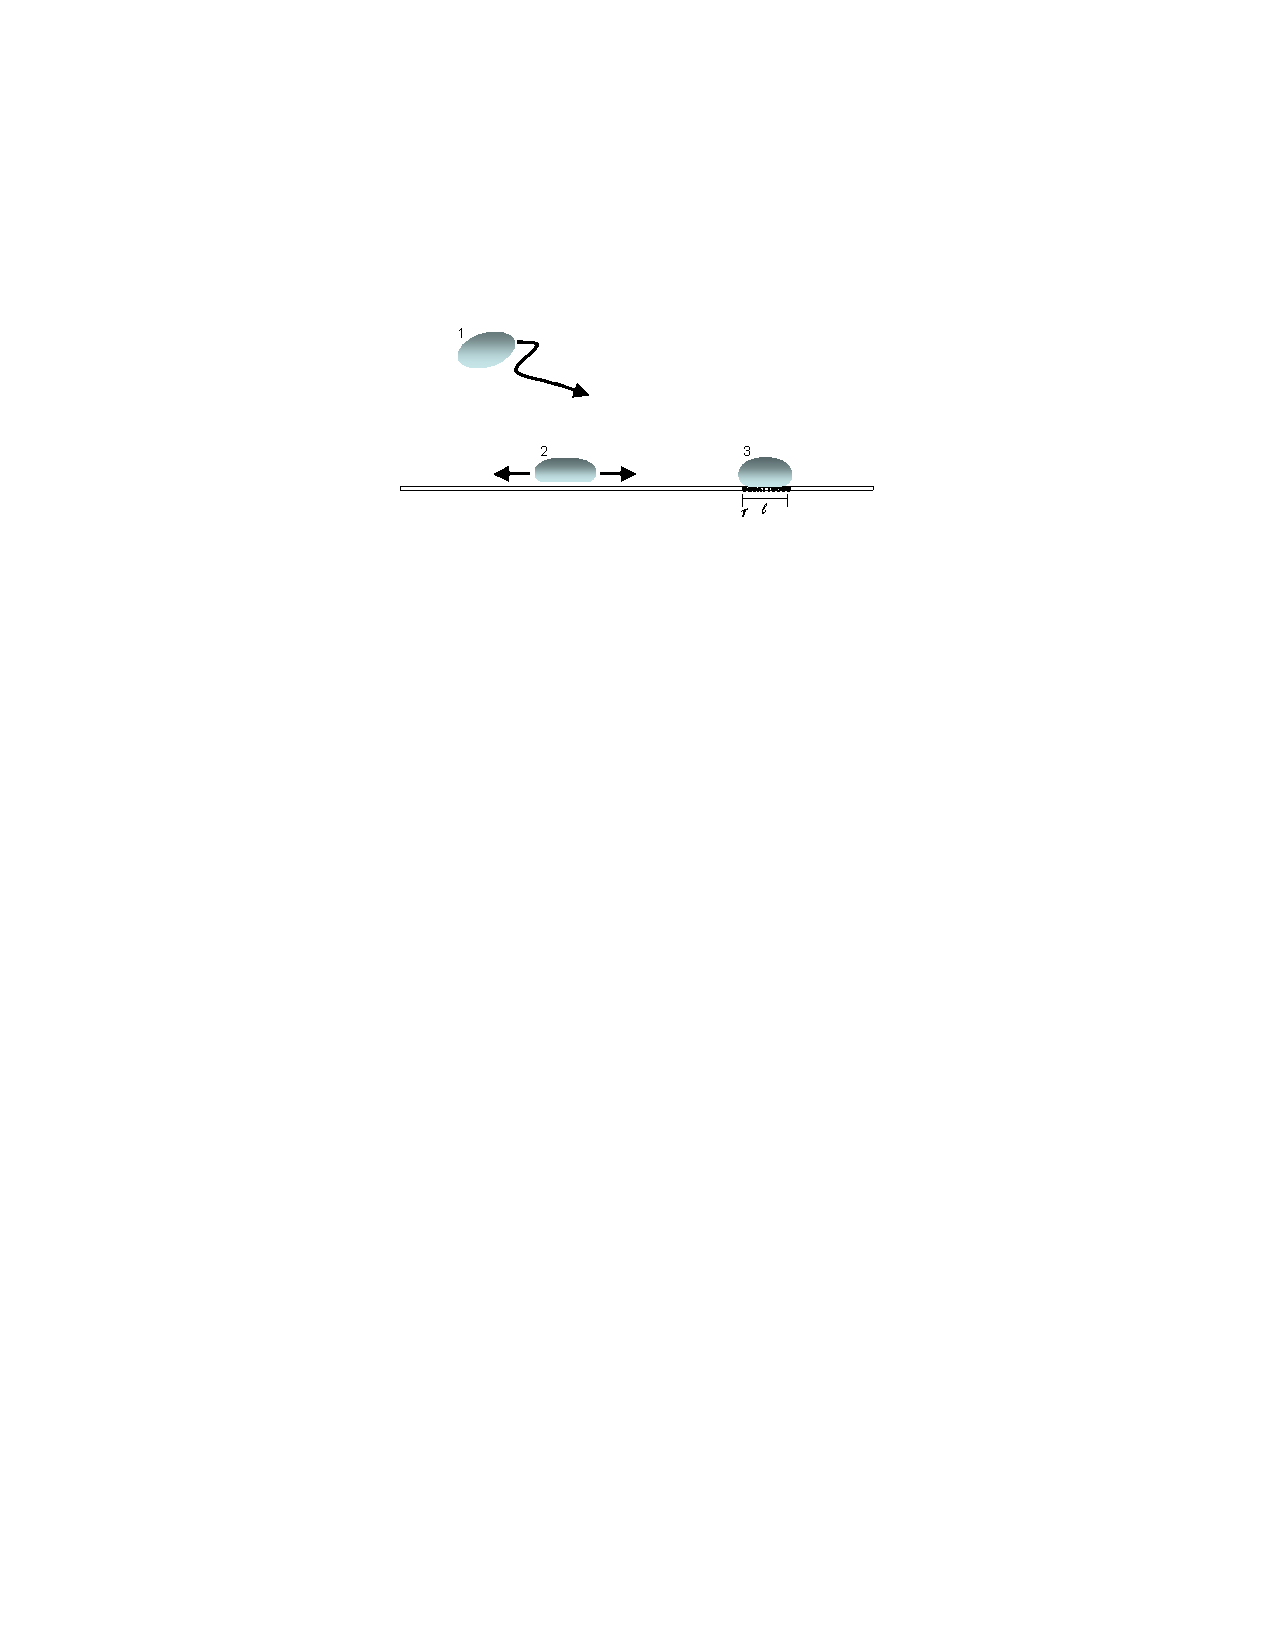
\includegraphics[width=0.8\textwidth]{figures/lassig-TF-search.pdf}
\captionbf{Diff�rents �tats du \tf}{
Figure tir�e de \cite{Lassig2007p539}. Lors de sa recherche de site de
fixation, le TF peut se trouver dans trois �tats distincts : (1) un �tat libre
de diffusion tridimensionnelle, (2) un �tat de diffusion unidimensionnelle sur
l'ADN par fixation non sp�cifique, et (3) un �tat de fixation sp�cifique.
L'�nergie de fixation d�pend du site de fixation, de taille $l$ et de
coordonn�e $r$.
}
\label{fig:lassig-TF-search}
\efig


\subsection{Modes de recherche du site de fixation par le TF}
\label{sub:modes_de_recherche_du_site_de_fixation_par_le_tf}

Un \ft peut �tre dans plusieurs �tats : en diffusion tridimensionnelle, auquel
cas il est dit \og libre \fg, ou bien fix� sur l'ADN. Dans ce dernier cas, il
interagit avec l'ADN selon deux modes : une attraction non sp�cifique d'�nergie
$E_{ns}$ ind�pendante de la position sur l'ADN, et une interaction sp�cifique
$E_s(r)$ qui d�pend de la s�quence de taille $l\sim10$ � la position $r$ sur
l'ADN.  L'interaction non sp�cifique est due � l'interaction �lectrostatique
entre la prot�ine charg�e positivement et l'ADN charg� n�gativement, alors que
l'interaction sp�cifique implique des liaisons hydrog�nes entre le domaine de
fixation de la prot�ine et les nucl�otides du site de fixation. 
%La prot�ine
%passe d'un mode � l'autre en changeant de conformation. 
Le \tf peut ainsi se
trouver dans trois �tats thermodynamiques repr�sent�s en figure
\ref{fig:lassig-TF-search} : en diffusion tridimensionnelle libre, fix� non
sp�cifiquement (diffusion unidimensionnelle le long de la structure d'ADN), et
fix� sp�cifiquement sur l'ADN. Ces trois modes contribuent � la cin�tique de la
recherche d'un site fonctionnel \cite{Berg1981kx,Winter1981fk,Winter1981uq}.
Ainsi, l'attraction non sp�cifique conduit la prot�ine � passer � peu pr�s
autant de temps fix� sur l'ADN qu'en diffusion libre. La recherche de site de
reconnaissance est donc un processus mixte de diffusion unidimensionnelle sur
l'ADN et de diffusion tridimensionnelle dans le milieu. Lorsqu'il est fix� sur
l'ADN, le facteur diffuse dans un paysage d'�nergie $E_{ns}$ plat lorsqu'il est
dans sa conformation de fixation non sp�cifique, ou dans un paysage d'�nergie
$E_s(r)$ dans sa conformation de fixation sp�cifique. Cela permet au facteur
d'�chantillonner les sites de faible �nergie $E_s(r)$ tout en �vitant d'�tre
bloqu� par les barri�res de haute �nergie en passant en mode de recherche non
sp�cifique. Ce processus s'av�re au final tr�s efficace : les temps de
recherche sont typiquement inf�rieurs � une minute, ce qui est petit devant les
processus de r�gulation de la cellule qui se d�roulent au mieux sur quelques
minutes~\cite{Gerland2002p397,Slutsky2004vn}. Il est donc pertinent de d�crire
l'effet d'un site de fixation sur la r�gulation d'un g�ne cible par la
probabilit� qu'il a de fixer un \tf � l'�quilibre thermodynamique.


% subsection modes_de_recherche_du_site_de_fixation_par_le_tf (end)

\subsection{Mod�le PWM} 
\label{sub:modele_pwm}
Pr�sent� en 1987 par Berg et von Hippel~\cite{Berg1987p3746}, le mod�le PWM est
le mod�le le plus simple d�crivant l'�nergie de fixation sp�cifique entre un \tf et un
site de fixation sur l'ADN.  Ce mod�le repose sur plusieurs hypoth�ses. Tout
d'abord, il y a l'hypoth�se importante que les sites de fixation des TFs sur
l'ADN ont �t� s�lectionn�s au cours de l'�volution pour leur propri�t� de sites
de reconnaissance, quelle que soit la concentration du TF dans la cellule. En
d'autres termes, le processus de s�lection discrimine les sites de fixation sur
la seule base de leur �nergie de fixation � un TF donn� : les sites ayant une
�nergie de fixation dans une certaine gamme sont retenus, les autres rejet�s.  Par
ailleurs, au sein de cette gamme d'�n�rgie \og utile \fg, toutes les s�quences
sont �quiprobables. Enfin, la derni�re hypoth�se est que chaque nucl�otide d'un
site de fixation contribue de mani�re ind�pendante, \cad additive � l'�nergie
totale du site.  Cette hypoth�se permet de simplifier le probl�me en gardant le
nombre de param�tres petit. 

\bfigp
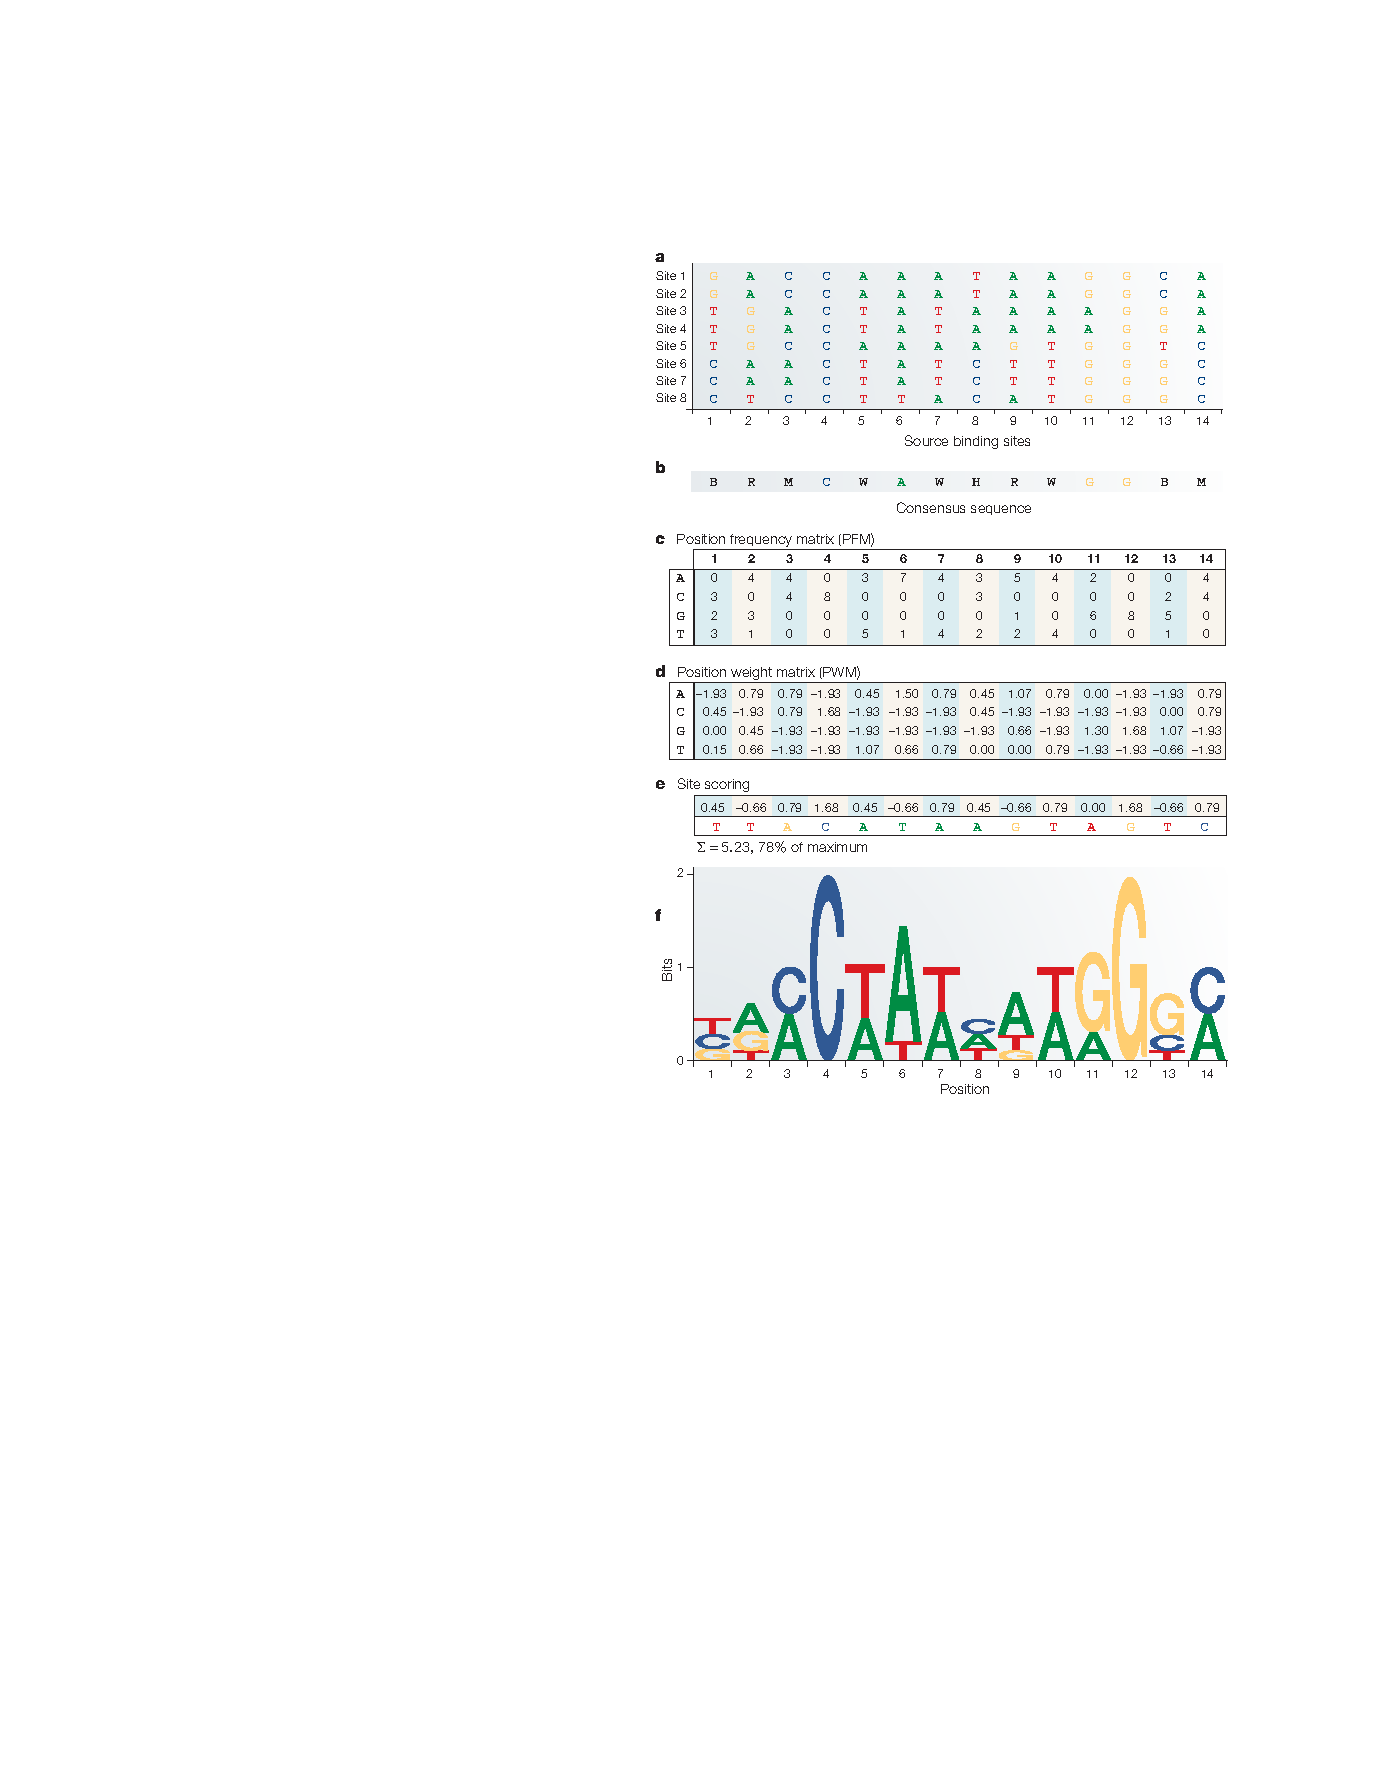
\includegraphics[width=.7\textwidth]{figures/wasserman-PWM.pdf}
\captionbf{Construction et utilisation du mod�le PWM}{
    Figure tir�e de \cite{Wasserman2004p624}. (a) Supposons connus un certain nombre
    de sites de fixation d'un \tf (dans ce cas MEF2). (b) S�quence consensus
    correspondante utilisant les symboles IUPAC. (c) Une matrice de fr�quence
    est construite, indiquant pour chaque nucl�otide sa multiplicit� � une
    position donn�e dans le site. (d) La PWM est simplement construite en
    prenant le logarithme relatif des fr�quences PWMs par rapport aux fr�quences
    \apriori des nucl�otides. (e) Le score (ou �nergie) d'une s�quence d'ADN
    donn�e est calcul� en additionnant les poids PWM correspondants. (f) La PWM
    peut �tre repr�sent�e sous forme de logo \cite{Giocomo2011p3442}. Dans cette
    repr�sentation, la hauteur d'une colonne repr�sente le contenu en
    information ou information relative moyenne d'une position, et la taille des
    bases refl�te leur fr�quence.

} 
\label{fig:wasserman-PWM}
\efigp


L'argument de Berg et von Hippel est que ce probl�me est analogue � celui de
physique statistique consistant � d�duire les taux d'occupation des niveaux
d'�nergie de particules ind�pendantes sachant que l'�nergie totale doit avoir
une certaine valeur moyenne $E$. La solution de ce probl�me est donn�e par la
formule de Boltzmann reliant �nergie et taux d'occupation :

\begin{equation} 
    f_{i,b} = \exp(-\lambda E_{i,b}) / \Z_i
    \label{eq:boltzmann}
\end{equation}

o� $f_{i,b}$ est la probabilit� d'observer la base $b$ � la position $i$ du
site de fixation, $E_{i,b}$ est l'�nergie associ�e (en $k_BT$), $\Z_i$ est la
fonction partition qui permet de normaliser la distribution � la position $i$,
et $\lambda$ est un facteur sans dimension, analogue du $\beta$ de la
thermodynamique, et li� au processus de s�lection. Dans la suite, nous
int�grerons ce facteur � l'�nergie.  \\ La connaissance des fr�quences des
bases permet de d�finir une autre quantit� utile caract�risant la variabilit�
des s�quences de fixation, l'information relative des sites par rapport � une
s�quence d'ADN al�atoire~\cite{Stormo1998p471}:

\begin{equation} 
    \mathcal{I} = \sum_{i=1}^{L}\sum_{b = A,C,G,T}^{}f_{i,b}\ln\left(\frac{f_{i,b}}{\pi_b}\right) 
\end{equation}

o� $L$ est la taille du site de fixation et $\pi_b$ correspond � la probabilit�
\apriori d'observer la base $b$ dans le g�nome. 
%Parce que l'�nergie est d�finie
%� une constante pr�s, 
Il est usuel de d�finir l'�nergie relativement au fond g�nomique
: 

\begin{equation} 
    \tilde{E}_{i,b} = \ln\left(\frac{f_{i,b}}{\pi_b}\right) 
\end{equation}

L'�nergie totale d'un site $S_i$ est alors

\begin{equation}
    \begin{aligned}
        E &= \sum_{i=1}^{L}\tilde{E}_{i,b} \\
        &= \sum_{i=1}^{L}\ln\left(\frac{f_{b(i)}}{\pi_b}\right)\\
        &=\ln\left(\frac{\prod_{i=1}^{L}f_{b(i)}}{\prod_{i=1}^{L}\pi_b}\right)\\
        &=\ln\left(\frac{P(S_i|\text{TF})}{P(S_i|\text{fond g�nomique})}\right)
    \end{aligned}
\end{equation} 

o� $b(i)$ est la base situ�e � la position $i$ du site de fixation. Cette
�nergie quantifie simplement � quel point la s�quence $S_i$ est plus ($E>0$) ou
moins ($E<0$) probablement un site de fixation (de probabilit�
$P(S_i|\text{TF})$) qu'un site tir� au hasard dans le g�nome (de probabilit�
$P(S_i|\text{fond g�nomique})$). On parle aussi de \textit{score} de la
s�quence. L'information relative $\mathcal{I}$, qui est le score moyen des s�quences
fix�es par le TF,  peut alors �tre vue comme quantifiant � quel point
l'ensemble des sites de fixation se distingue d'un ensemble de m�me taille de
sites tir�s au hasard.

Avec ces outils en main, il devient alors simple de b�tir un mod�le PWM et de
l'utiliser pour pr�dire des s�quences fix�es (fig.~\ref{fig:wasserman-PWM}).
�tant donn�s des sites de fixation connus, il suffit d'�valuer la fr�quence
d'occurrence de chaque base � chaque position. La comparaison avec les
probabilit�s g�nomiques \apriori d'occurrence permet alors de b�tir une matrice
de score, la PWM. Cette matrice peut alors �tre utilis�e pour attribuer un
score � une s�quence d'ADN en additionnant les scores � chaque position.
Finalement, les s�quences ayant un score d�passant un certain seuil sont
consid�r�es comme des s�quences de fixation.

\FloatBarrier
\subsection{Mod�le biophysique}
\label{sub:modele-biophys}

Le mod�le PWM est bas� sur une hypoth�se forte, celle que les sites de fixation
ont �t� s�lectionn�s sur la base de leur seule affinit� ou �nergie envers un
TF. N�anmoins, � aucun moment n'intervient la concentration du TF dans la
cellule, dont d�pend pourtant la probabilit� de fixation. C'est ce que tente de
capturer le mod�le
biophysique~\cite{Gerland2002p397,Djordjevic2003p2932,Zhao2009p3948}.  \\

Consid�rons l'interaction entre un TF et une s�quence d'ADN $S_i$ :

\begin{equation}
    TF+S_i \rightleftharpoons TF:S_i
\end{equation}

o� $TF:S_i$ d�note le complexe entre le TF et le site $S_i$. La constante d'�quilibre de cette r�action s'�crit selon la loi d'action de masse :

\begin{equation}
    \label{eq:TF-equilibrium}
    K_i = \frac{[TF:S_i]}{[TF][S_i]}
\end{equation}

Le site peut �tre dans deux �tats : occup� par le TF o� libre. Aussi, la probabilit� que le TF soit fix� au site s'�crit simplement

\begin{equation}
    P(\text{fixation}|S_i) = \frac{[TF:S_i]}{[TF:S_i]+[S_i]}
    = \frac{1}{1+\frac{1}{K_i [TF]}} = \frac{1}{1+e^{\beta(E_i-\mu)}}
    \label{eq:modele-biophys}
\end{equation}

o� $E_i=-kT\ln(K_i)$ est l'�nergie libre standard de fixation (souvent not�e
$\Delta G$), $\mu=kT\ln[TF]$ est le potentiel chimique, $k$ est la
constante de Boltzmann, $T$ la temp�rature et $\beta=1/kT$.  Ici nous avons
consid�r� qu'il n'y avait qu'un seul site de fixation. De mani�re g�n�rale, le
site est en comp�tition avec le fond g�nomique, ce qui ajoute une contribution
� $\mu$ (voir section \ref{sub:modele_thermodynamique}).  � l'instar du mod�le PWM,
l'�nergie $E_i$ est g�n�ralement prise comme �tant une fonction additive des
�nergies individuelles des diff�rentes bases du site. Ainsi, lorsque le TF est
� faible concentration ($\mu \to -\infty$), le mod�le biophysique �crit en
�quation~\ref{eq:modele-biophys} se r�duit au mod�le PWM.


\subsection{Mod�le thermodynamique} \label{sub:modele_thermodynamique} La
description biophysique peut �tre r��crite en termes thermodynamiques en
utilisant des raisonnements simples sur le nombre d'�tats possibles et leur
�nergie (et donc poids de Boltzmann) associ�e. Nous adoptons ici l'approche
de~\cite{Gerland2002p397}. On pourra par ailleurs se r�f�rer � l'excellente
revue~\cite{Lassig2007p539}.  Consid�rons le cas simple d'un seul \ft
interagissant avec un g�nome de taille $L \gg 1$ ne contenant qu'un seul site
fonctionnel, le reste de la s�quence �tant al�atoire. Nous l'avons vu,
l'exp�rience montre que la prot�ine se fixe � l'ADN avec une probabilit� $1/2$.
Lorsqu'elle est fix�e, elle est � l'�quilibre entre le mode sp�cifique et le
mode non sp�cifique. Nous d�sirons savoir avec quelle probabilit� elle est
fix�e de mani�re sp�cifique. La fonction de partition, �num�rant tous les poids
de Boltzmann associ�s aux diff�rents �tats accessibles au TF fix� s'�crit :

\begin{equation}
    \Z = \sum\limits_{r=1}^{L} e^{-\beta E_s(r)} + L e^{-\beta E_{ns}}
\end{equation}

Notons $i$ la position du site fonctionnel. On peut �crire :

\begin{equation}
    \begin{aligned}
        \Z & = e^{-\beta E_s(i)} + e^{-\beta E_{ns}} + \sum\limits_{r \neq i} e^{-\beta E_s(r)} + (L - 1) e^{-\beta E_{ns}}\\
    & \simeq e^{-\beta E_i} + \Z_0
\end{aligned}
\end{equation}

o� $Z_0$ est la fonction de partition d'une s�quence al�atoire, et nous avons introduit l'�nergie $E_i$ d�finie par

\begin{equation}
    e^{-\beta E_i} = e^{-\beta E_s(i)} + e^{-\beta E_{ns}}
    \label{eq:Ei}
\end{equation}

Dans le cas d'un site de reconnaissance, $E_{ns} \gg E_s(i)$ de sorte que $E_i
\simeq E_s(i)$~\cite{Gerland2002p397}. La probabilit� que le
facteur soit fix� sur le site fonctionnel s'�crit finalement :

\begin{equation}
    P(\text{fixation sp�cifique}|E_i) = \frac{e^{-\beta E_i}}{\Z} = \frac{1}{1+e^{\beta (E_i-F_0)}}
    \label{eq:fixation-un-tf}
\end{equation}

o� $F_0 = - kT \log \Z_0$ est l'�nergie libre d'une s�quence g�nomique al�atoire.
On reconnait une fonction de Fermi, avec un seuil d'�nergie � $F_0$ : pour $E_i
< F_0$, la prot�ine est essentiellement fix�e de mani�re sp�cifique � son site
de reconnaissance, alors que pour $E_i > F_0$, elle ne distingue plus le site
du fond g�nomique et y est faiblement fix�e.\\

G�n�ralisons � pr�sent au cas de plusieurs \fts et sites de reconnaissance.
Nous n�gligeons le recouvrement entre \fts fix�s sur des sites proches, qui
poserait des probl�mes st�riques et corr�lerait les sites de fixation dans un
certain voisinage (la pr�sence d'un TF emp�chant la pr�sence d'un autre), et
consid�rons que le nombre de TFs est grand devant le nombre de sites de
reconnaissance pour �viter les probl�mes de saturation : ainsi, le g�nome est
compos� de $L$ s�quences ind�pendantes, chacune pouvant �tre soit non occup�e,
soit occup�e de mani�re non sp�cifique, soit occup�e de mani�re sp�cifique.
Notons $\mu$ le potentiel chimique du TF en solution. La fonction de partition
totale est le produit des fonctions de partition des sites ind�pendants,

\begin{equation}
    \Z(\mu) = \prod\limits_{r=1}^{L}\Z(\mu,r)
\end{equation}

o� la fonction de partition d'un site s'�crit :

\begin{equation}
    \Z(\mu,r) = e^{-\beta \mu} + e^{-\beta E_s(r)} + e^{-\beta E_{ns}}
\end{equation}

En utilisant � nouveau la d�finition de $E_i$ en �q.\ref{eq:Ei}, la probabilit�
de fixation d'un site � la position $i$ s'�crit

\begin{equation}
    P(\text{fixation sp�cifique}|E_i) = \frac{e^{-\beta E_i}}{\Z(\mu,i)} = \frac{1}{1+e^{\beta (E_i-\mu)}}
\end{equation}

La valeur de $\mu$ est li�e � la fois au nombre de TFs ainsi qu'� la
possibilit� de se fixer dans le fond g�nomique. Elle est fix�e implicitement
par l'�quation :

\begin{equation}
    n = \sum_{r=1}^{L} \frac{1}{1+e^{\beta (E_r - \mu)}}
\end{equation}

qui signifie simplement que le nombre de TFs $n$ dans le syst�me est �gal � la
somme sur tous les sites de fixation possibles pond�r�e par la probabilit� que
le TF y soit fix�. Lorsque $\mu \to -\infty$ et que la fonction de Fermi peut
�tre approxim�e par la loi de Boltzmann, l'�quation peut s'inverser et l'on
trouve~\cite{Aurell2007p3747}

\begin{equation}
    \mu = F_0 + kT \log n
\end{equation}

o� $F_0$ est l'�nergie libre du fond g�nomique introduite en
�q.~\ref{eq:fixation-un-tf}. Ainsi, la prise en compte d'une multiplicit� de
TFs ajoute un facteur $kT \log n$ au seuil de la fonction de Fermi par rapport
au cas d'un seul TF. Par ailleurs, cette approche thermodynamique nous a permis
de g�n�raliser le mod�le biophysique simple introduit en section
\ref{sub:modele-biophys}.

\FloatBarrier
\section{Les interactions prot�ine-ADN : mesures exp�rimentales}
\label{sec:mesures_exp}

Ces derni�res ann�es, des avanc�es technologiques consid�rables ont permis
d'une part d'�tablir des mod�les de fixation sp�cifique pour de nombreux TFs,
d'autre part de localiser leurs sites de fixation dans le g�nome. Ces avanc�es
ont eu lieu autant sur le plan \invitro, utilisant prot�ines purifi�es et
s�quences nucl�iques artificielles pour d�duire l'affinit� prot�ine-ADN, que
sur le plan \invivo, mesurant l'interaction de la prot�ine avec l'ADN
g�nomique~\cite{Stormo2010p3947}. 

\subsection{Approches \invitro : MITOMI, SPR, PBM, CSI, SELEX, et HT-SELEX}
\label{sub:approches_invitro}

\subsubsection{Approche microfluidique : MITOMI}

En 2007, Maerkl et Quake ont mis au point une technique appel�e MITOMI
(Mechanically Induced Trapping Of Molecular Interactions) permettant une mesure
directe de l'affinit� d'un TF � des centaines de s�quences d'ADN � la
fois~\cite{Maerkl2007p840}.  Cette technique repose sur l'utilisation d'un
syst�me microfluidique compos� de chambres dans lesquelles un fluide dont on
peut facilement modifier la composition circule dans des canaux d'un diam�tre
de l'ordre de $1\mu$m dont le microenvironnement est finement contr�l�.  Le
fluide contient des g�nes synth�tiques codant pour le TF ainsi que du mat�riel
permettant la synth�se de la prot�ine directementau sein de la chambre, ce qui
�vite de purifier pr�alablement le TF. Chaque chambre du syst�me contient des
anticorps fix�s � la surface permettant de capturer le TF et une certaine
concentration d'une s�quence d'ADN sp�cifique contenant une marque
fluorescente. Le syst�me contient ainsi des centaines de s�quences d'ADN
diff�rentes, chacune �tant pr�sente � diff�rentes concentrations. Lorsque le TF
est fix� par les anticorps, il recrute des s�quences d'ADN selon leur affinit�.
Celles qui ne se fixent pas sont lav�es. Au final, les s�quences fix�es
produisent un signal de fluorescence. La comparaison des signaux pour
diff�rentes concentrations d'ADN donne acc�s au rapport des constantes
d'�quilibre $K_{eq}$ (eq.~\ref{eq:TF-equilibrium}). La comparaison avec une
s�quence r�f�rence dont la constante $K_{eq}$ est connue permet alors de
d�terminer le $K_{eq}$ absolu pour chaque s�quence de fixation.  \\ 

En utilisant $17$ syst�mes de ce type, ils ont ainsi pu mesurer l'affinit� de
$4$ TFs de type bHLH � $464$ s�quences d'ADN diff�rentes: les s�quences
consensus et des s�quences ayant une, deux, trois ou quatre mutations. � titre
de comparaison, ils ont construit une PWM � partir des s�quences contenant une
seule mutation, puis ont pr�dit les �nergies attendues des s�quences
� plusieurs mutations. La pr�diction de la PWM s'est av�r�e bonne dans
seulement $56\%$ des cas pour les s�quences � deux mutations, $10\%$ pour les
s�quences � $3$ mutations et $0\%$ des cas pour les s�quences � $4$ mutations,
montrant les limites de ce mod�le ind�pendant confront� � des donn�es
d'interactions d'ordre sup�rieur. Un mod�le plus raffin� prenant en compte
l'�nergie d'interaction non sp�cifique et incluant des interactions entre
nucl�otides voisins permet n�anmoins de rendre compte des valeurs
observ�es~\cite{Stormo2007bh}. Nous reviendrons sur la n�cessit� de prendre en
compte les interactions entre paires de nucl�otides lors de l'interaction
sp�cifique entre TF et ADN dans le chapitre~\ref{ch:maxent}.

\subsubsection{Approche physique : la microscopie SPR}

La m�thode de r�sonance des plasmons de surface (\textit{Surface Plasmon
Resonance} ou SPR) est habituellement utilis�e pour �tudier l'interaction d'une
prot�ine avec un ligand (qui peut �tre une autre prot�ine), mais elle peut
aussi �tre utilis�e pour mesurer les interactions entre une prot�ine et
quelques centaines de s�quences d'ADN
diff�rentes~\cite{Shumaker-Parry2004ve,Campbell2007ly}. Le principe de la
microscopie SPR est que l'angle de r�flection de la lumi�re sur une fine
surface d'or, par exemple, d�pend de la masse de mol�cules fix�es de l'autre
c�t� de sa surface. Si de l'ADN est li� � la surface, la fixation du TF induit
un changement de masse et donc d'angle de reflection lumineuse mesurable au
cours du temps. Ainsi, la cin�tique de fixation du TF jusqu'� l'atteinte de
l'�quilibre est accessible. On peut de m�me �tudier la dissociation du TF lors
du lavage de la surface. Ces mesures donnent directement acc�s aux taux
d'association $k_{on}$ et de dissociation $k_{off}$ que la simple mesure de la
constante d'�quilibre $K_{eq}=k_{on}/k_{off}$ ne permet habituellement pas de
d�terminer.

\subsubsection{Approches bas�es sur des puces � ADN : PBM et CSI}

L'analyse de fixation des prot�ines par puce � ADN (\textit{Protein-Binding
Microarray} ou PBM) est une technologie haut d�bit qui a �t� d�velopp�e au
cours des 10 derni�res ann�es~\cite{Berger2006qf}. Les puces sont compos�es de
$44,000$ puits auxquels sont li�s des brins d'ADN. Une puce contient tous les
sites de fixation de $8$bp possibles ($4^8/2=32,768$ s�quences en prenant en
compte le fait qu'il y a un site sur chacun des deux brins d'ADN) plus deux bases
flanquantes (une � chaque extr�mit�) qu'il est possible de faire varier. Un
TF purifi� � partir de cellules ou synth�tis� \invitro est ajout� � la puce,
qui est ensuite lav�e pour se d�barrasser des fixations non sp�cifiques. La
quantit� de prot�ine fix�e � un puits donn� est d�termin�e gr�ce � un anticorps
fluorescent contre la prot�ine. L'enrichissement en prot�ine est calcul�
relativement au bruit de fond (anticorps non sp�cifique par exemple). Il est
alors possible d'utiliser ces mesures pour b�tir une PWM du TF (voir par
exemple~\citet{Kinney2007p3977}).\\

Une autre m�thode utilise aussi des puces � ADN : c'est l'identification de
site apparent� (\textit{Cognate Site Identifier} ou CSI)~\cite{Warren2006cr}.
Une diff�rence technique avec les PBMs est que l'ADN est d'abord synth�tis� en
simple brin puis se replie en double brin pour former le site de fixation,
�vitant ainsi de devoir g�n�rer l'ADN double brin � partir de pr�curseurs. Par
ailleurs, le TF est en comp�tition avec un marqueur fluorescent qui peut se
fixer � l'ADN: il n'est donc pas n�cessaire d'utiliser un marquage sp�cifique
sur le TF ou sur un anticorps, ce qui rend la proc�dure plus g�n�ralisable.
Finalement, la sp�cificit� du TF est repr�sent�e par un \og paysage de
sp�cificit� \fg qui encapsule l'information de fluorescence de l'ensemble des
variations par rapport � une s�quence consensus dans une repr�sentation
simple~\cite{Carlson2010dq}.

\subsubsection{Approche par purification des s�quences fix�es : SELEX et HT-SELEX}

Mise au point il y a plus de $20$ ans, la m�thode SELEX (\textit{Systematic
Evolution of Ligands by EXponential enrichment}) repose sur la s�lection de
s�quences d'ADN al�atoires par un TF
\invitro~\cite{Oliphant1989nx,Tuerk1990qe,Blackwell1990ai,Wright1991dp}. Une
biblioth�que de sites de fixation potentiels est d'abord g�n�r�e en
synth�tisant des s�quences d'ADN al�atoires ou en utilisant des s�quences
g�nomiques. Les extr�mit�s de ces s�quences contiennent des pr�curseurs permettant
l'amplification exponentielle par PCR. Le TF purifi� est ajout� aux sites et
les s�quences fix�es sont s�par�es des s�quences non fix�es, par exemple par
retard sur gel. Apr�s un cycle de s�lection, les s�quences r�cup�r�es sont
encore enrichies en s�quences de basse affinit� pour le TF, car celles-ci sont
simplement initialement bien plus abondantes que les s�quences de haute
affinit�. Afin d'augmenter la proportion de s�quence de grande affinit�, les
s�quences filtr�es sont amplifi�es puis filtr�es � nouveau, ceci sur
plusieurs cycles. � la fin de ce processus, les s�quences s�lectionn�es sont
clon�es et s�quenc�es, r�sultant en un nombre typique de moins de $\sim100$
s�quences ind�pendantes~\cite{Fields1997yq}. Si les s�quences initiales sont
issues d'ADN g�nomique, il est possible d'utiliser l'hybridation des s�quences
� des puces � ADN. La pr�sence de plusieurs cycles de s�lection rend n�anmoins
la d�termination des �nergies de fixation moins directe qu'avec les techniques
pr�c�dentes. Une variante de la technique appel�e SELEX-SAGE utilise des
multim�res de sites � la place de sites uniques et permet de r�duire le nombre
de cycles de s�lection et d'augmenter ainsi le nombre de s�quences de fixation
obtenues~\cite{Roulet2002rt}, permettant de r�aliser des mod�les plus
pr�cis~\cite{Nagaraj2008p3749}.

Depuis la mise au point de la m�thode SELEX, des avanc�es consid�rables ont �t�
r�alis�es dans les techniques de s�quen�age, permettant l'obtention de millions
de s�quences � la fois : on parle de s�quence haut-d�bit
(\textit{high-throughput}) ou encore s�quen�age massivement parall�le.
L'utilisation de ces nouvelles techniques dans l'exp�rience SELEX a men� � la
m�thode HT-SELEX~\cite{Nagaraj2008p3749}, aussi appel�e
Bind-n-Seq~\cite{Zykovich2009gf}. Il est alors possible d'estimer un mod�le
d'�nergie � partir des fr�quences d'observation des diff�rentes s�quences d�s
le premier cycle~\cite{Nagaraj2008p3749}. Des cycles suppl�mentaires permettent
d'obtenir plus d'information sur les s�quences les plus sp�cifiques, notamment
sur la pr�sence de contributions non ind�pendantes � l'�nergie, ou de compenser
la faible sp�cificit� d'un TF. L'avantage de cette technique est que la taille
des sites de fixation n'est pas limit�e. Ainsi, avec une nanomole d'ADN
($\sim10^{15}$ s�quences) on peut couvrir l'ensemble des sites de $25$bp
possibles. Le s�quen�age haut-d�bit permet d'en �chantillonner $\sim10^8$, ce
qui est largement suffisant pour contraindre des mod�les d'�nergie
ind�pendants, m�me pour des TFs ayant des sites de fixations de taille $>15$bp
comme c'est souvent le cas chez la bact�rie. Cette technique a r�cemment �t�
pouss�e encore plus loin~\cite{Jolma2010ul}. En utilisant des prot�ines
marqu�es, les auteurs ont r�alis� un HT-SELEX � partir d'extraits cellulaires,
et en ajoutant un code barre aux s�quences d'ADN de chaque exp�rience, ils ont
pu analyser les sites de fixation pour plusieurs TFs en parall�le. Ils ont
ensuite utilis� cette technique pour obtenir des mod�les de sp�cificit� pour
$411$ TFs humains, la plus grande �tude de ce genre r�alis�e � ce
jour~\cite{Jolma2013p3971}.






\subsection{Approche clonale : la technique de simple hybride}
\label{sub:approche_clonale_la_technique_de_simple_hybride}

Contrairement aux approches pr�c�dentes, la technique de simple hybride
(\textit{Bacterial one-hybrid} ou B1H) n'est pas purement \invitro, au sens o�
l'interaction prot�ine-ADN est test�e au sein d'une bact�rie.  N�anmoins, parce
que l'interaction n'est pas test�e dans son contexte cellulaire d'origine, nous
la consid�rerons comme telle. Cette approche repose sur l'int�gration par une
bact�rie h�te de deux vecteurs d'expression g�n�tique, ou plasmides. Le premier
exprime le \tf d'int�r�t fusionn� � une sous-unit� de l'ARN polym�rase
(l'app�t), c'est la prot�ine \og hybride \fg. L'autre contient une r�gion de
s�quence al�atoire repr�sentant un site de fixation potentiel (la proie) en
amont d'un promoteur � faible activit�. La fixation de cette r�gion par la
prot�ine hybride permet l'activation d'un g�ne de s�lection, g�n�ralement
\textit{HIS3}, un g�ne de la levure requis pour la biosynth�se de l'histidine
et dont l'homologue bact�rien est absent de la souche d'\ecoli utilis�e. La
croissance des cellules a lieu dans un milieu ne contenant pas l'histidine.
Dans ces conditions, les bact�ries n'exprimant pas \textit{HIS3} ne peuvent
cro�tre. Ainsi, seules les bact�ries au sein desquelles le \tf se fixe � la proie
expriment \textit{HIS3}, croissent et forment des colonies, d'o� la notion de
g�ne de s�lection. Par ailleurs, la stringence de la s�lection peut �tre
modul�e en ajoutant au milieu diff�rentes concentrations de 3-amino-triazole
(3-AT), un inhibiteur de \textit{HIS3}. De cette fa�on l'affinit� du site de
fixation peut �tre estim�e plus finement.  
\\ 

Dans les �tudes de ce type, les sites de fixation pr�sents au sein des colonies
sont s�quenc�s individuellement, ce qui permet d'obtenir environ $50$ s�quences
pour une exp�rience de s�lection donn�e. N�anmoins, il semble possible
d'utiliser les nouvelles technologies de s�quen�age pour r�cup�rer l'ensemble
des sites de fixation des bact�ries pr�sentes sur une
plaque~\cite{Stormo2010p3947}.  � l'instar de la m�thode HT-SELEX, on obtient
des millions de sites, ceux ayant une plus grande affinit� �tant pr�sents
� plusieurs centaines de milliers d'exemplaires, et ceux ayant une faible
affinit� �tant pr�sent en un seul voire aucun exemplaire.
\\

Notons qu'il est aussi possible d'adopter la d�marche inverse, \cad de partir
de quelques sites de fixation pr�sum�s fonctionnels mais pour lesquels on ne
conna�t pas le TF associ�. En utilisant une biblioth�que de plasmides codant
pour diff�rents TFs hybrides, il est alors possible de d�terminer si l'un
d'entre eux poss�de une affinit� importante avec les sites test�s.

% subsection approche_clonale_la_technique_de_simple_hybride (end)
\subsection{Approches \invivo : \chipchip, \chipseq, DNAse I}
\label{sub:chip_DNAseI}

Dans cette section, nous nous int�ressons aux techniques permettant
d'identifier les sites de fixation d'un \tf sur le g�nome. Ces m�thodes se
basent sur des extraits cellulaires (de $10^4$ � $10^8$ cellules) qui peuvent
provenir d'un tissu homog�ne (un seul type de cellule) ou h�t�rog�ne (plusieurs
types de cellules), voire de l'organisme entier si la dissection est impossible
(embryon de mouche par exemple). L'information obtenue est donc toujours
conditionn�e par ce mat�riau de d�part, et l'on n'obtient que les sites
\textit{accessibles} �tant donn�s le type cellulaire et la p�riode de
d�veloppement �tudi�s.

\bfigp
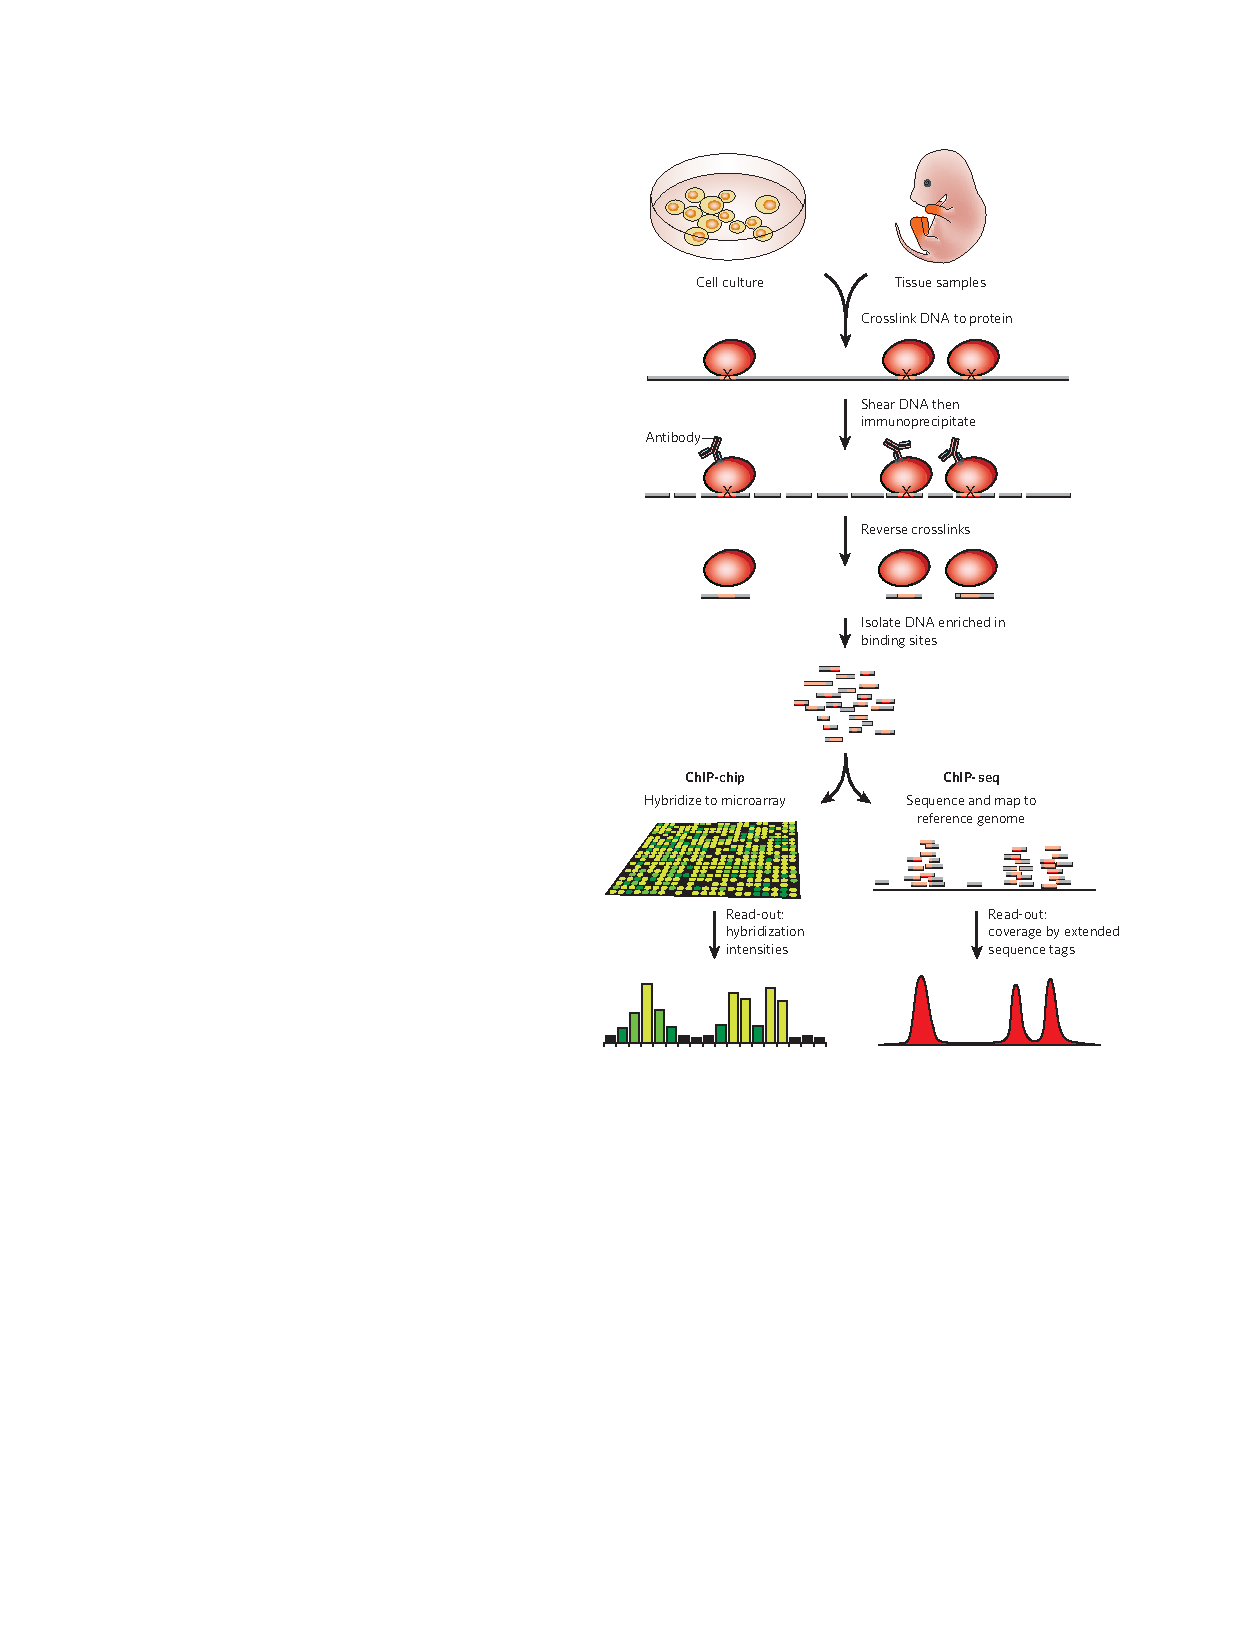
\includegraphics[width=0.6\textwidth]{figures/visel-chipseq.pdf}
\captionbf{�tapes d'une exp�rience de \chipchip et \chipseq}{

    Figure tir�e de~\citet{Visel2009kx}. � partir d'extraits cellulaires issus
    de cultures \invitro ou pr�lev�s \invivo, plusieurs �tapes permettent de
    r�cup�rer les r�gions fix�es par un TF d'int�r�t. D'abord, les prot�ines,
    li�es de mani�re non covalente � l'ADN, sont fix�es par utilisation d'un
    agent de r�ticulation, le formald�hyde. Puis la chromatine est d�coup�e en
    fragments de $\sim 500$bp par utilisation d'ultrasons : on parle de
    sonication. L'utilisation d'un anticorps sp�cifique au TF d'int�r�t permet
    de pr�cipiter les fragments d'ADN fix�s. Les fragments r�sultants sont
    alors soit hybrid�s � une puce � ADN contenant de nombreuses s�quences
    g�nomiques (\chipchip), soit directement s�quenc�s et align�s � un g�nome
    de r�f�rence (\chipseq). La comparaison � un �chantillon d'ADN non
    pr�cipit� (\og input \fg) permet alors de d�finir les r�gions
    significativement fix�es, avec une r�solution plus pr�cise dans le cas du
    \chipseq, o� l'ensemble du g�nome est couvert, par rapport au \chipchip,
    pour lequel seulement un sous ensemble du g�nome est analys�.

}
\label{fig:visel-chip}
\efigp

\subsubsection{Immunopr�cipitation de la chromatine : \chipchip et \chipseq}


La technique d'immunopr�cipitation de la chromatine (ChIP)
(fig.~\ref{fig:visel-chip}) consiste dans un premier temps � induire la
r�ticulation (\textit{crosslink}) des prot�ines se liant � l'ADN en
traitant les cellules avec de la formald�hyde. Cette �tape permet de
transformer les liaisons faibles prot�ine-ADN en liaisons covalentes. Une fois
les prot�ines fix�es, la chromatine est d�coup�e par digestion enzymatique ou
en la soumettant � des ultrasons (c'est la sonication), r�sultant en des
fragments de taille variant entre $200$ et $600$bp. Ces fragments sont ensuite
immunopr�cipit�s en pr�sence d'un anticorps sp�cifique d'un \tf ou d'un
isoforme d'histone (dans le cas d'une �tude du paysage �pig�n�tique) d'int�r�t,
permettant ainsi de r�cup�rer tous les sites de fixation dans le g�nome. Apr�s
purification des fragments pr�cipit�s, l'�chantillon peut �tre analys� soit par
hybridation sur puce (\chipchip) ou par s�quen�age haut d�bit (\chipseq).\\

Dans le cas du \chipchip, l'�chantillon immunopr�cipit� et l'ADN de d�part
(\textit{input}) sont marqu�s avec des colorants fluorescents et hybdrid�s
sur une puce � ADN compos�e de tr�s nombreux puits contenant des
oligonucl�otides (courtes s�quences d'ADN) correspondant � diff�rentes r�gions
du g�nome. Dans le meilleur cas, ces oligonucl�otides couvrent l'ensemble du
g�nome. Les sites de liaison sont identifi�s par l'�cart d'intensit� entre les
signaux de fluorescence des conditions d'immunopr�cipitation et
d'\textit{input}.
\\

\bfig
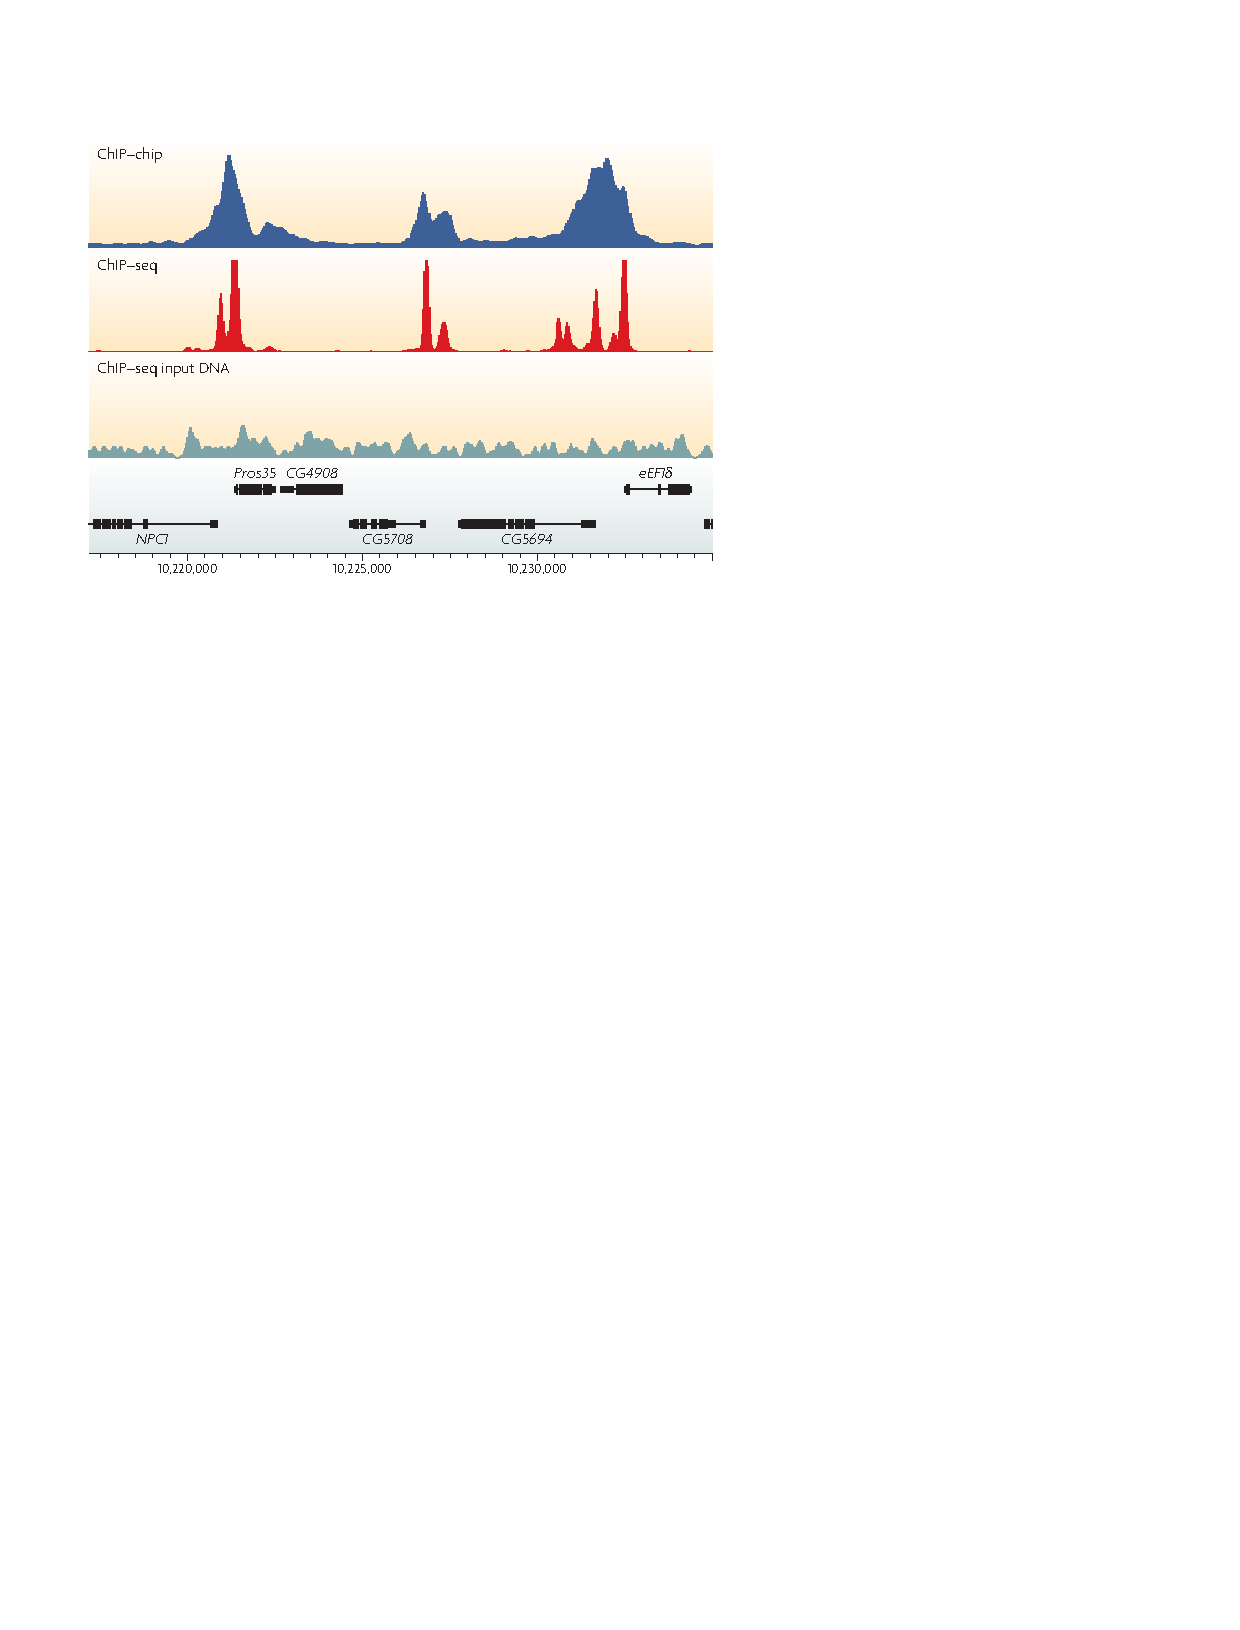
\includegraphics[width=0.8\textwidth]{figures/park-chip-resolution.pdf}
\captionbf{R�solution des exp�riences \chipchip et \chipseq}{
Figure tir�e de \cite{Park2009kx}, montrant les profils de fixation de la
prot�ine Chromator g�n�r�s � partir d'exp�riences de \chipchip
(intensit� relative par rapport au contr�le, bleu) et de \chipseq (densit� de
s�quences, rouge) dans la lign�e cellulaire S$2$ de \dmel. On peut noter la plus
grande r�solution de l'exp�rience \chipseq pour d�terminer les sites de
liaison. L'ADN utilis� en \textit{input} de l'exp�rience de \chipseq et servant
de contr�le est montr� en gris, et les g�nes du locus indiqu�s en noir.
}
\label{fig:park-chip-resolution}
\efig

Dans le cas du \chipseq, l'�chantillon immunopr�cipit� est analys� par
s�quen�age � haut d�bit, r�sultant en une librairie de \textit{reads} d'une
longueur typique variant entre $27$ et $50$bp issus des extr�mit�s des s�quences.
Ces \textit{reads} sont ensuite align�s sur un g�nome de r�f�rence. � chaque
position du g�nome correspond ainsi un certain nombre de s�quences pr�cipit�es
et d'\textit{input}. En comparant ce nombre au nombre moyen dans le locus et
� l'\textit{input}, il est possible d'identifier des pics correspondant � la
fixation du facteur (voir par exemple le programme d'appel de pics \chipseq
MACS \cite{Zhang2008uq}).  \\

Dans les deux cas, il faut noter que l'on a affaire � la fixation
\textit{moyenne} du facteur sur l'ADN dans la population de cellules �tudi�e.
Ainsi, un petit pic peut repr�senter aussi bien une fixation forte dans un
petit sous-ensemble de cellules (par exemple celles qui sont � un certain �tat
d'avancement du cycle cellulaire) qu'une fixation moyenne dans l'ensemble de la
population. L'exp�rience de \chipseq offre une r�solution bien plus pr�cise
($\leq100$bp) que la m�thode \chipchip (fig.~\ref{fig:park-chip-resolution}).
En effet, dans ce dernier cas la r�solution est limit�e par le nombre
d'oligonucl�otides utilis�s, qui sont dans le meilleur des cas r�partis sur le
g�nome avec $35-100$ nucl�otides d'�cart entre deux instances. Pour se comparer
� la \chipseq, il faudrait que tous les oligonucl�otides se superposent � une
base pr�s, ce qui demanderait un trop grand nombre de puces.


\FloatBarrier
\subsubsection{Empreinte � la DNase I (\textit{DNase I footprinting})}

\bfigp
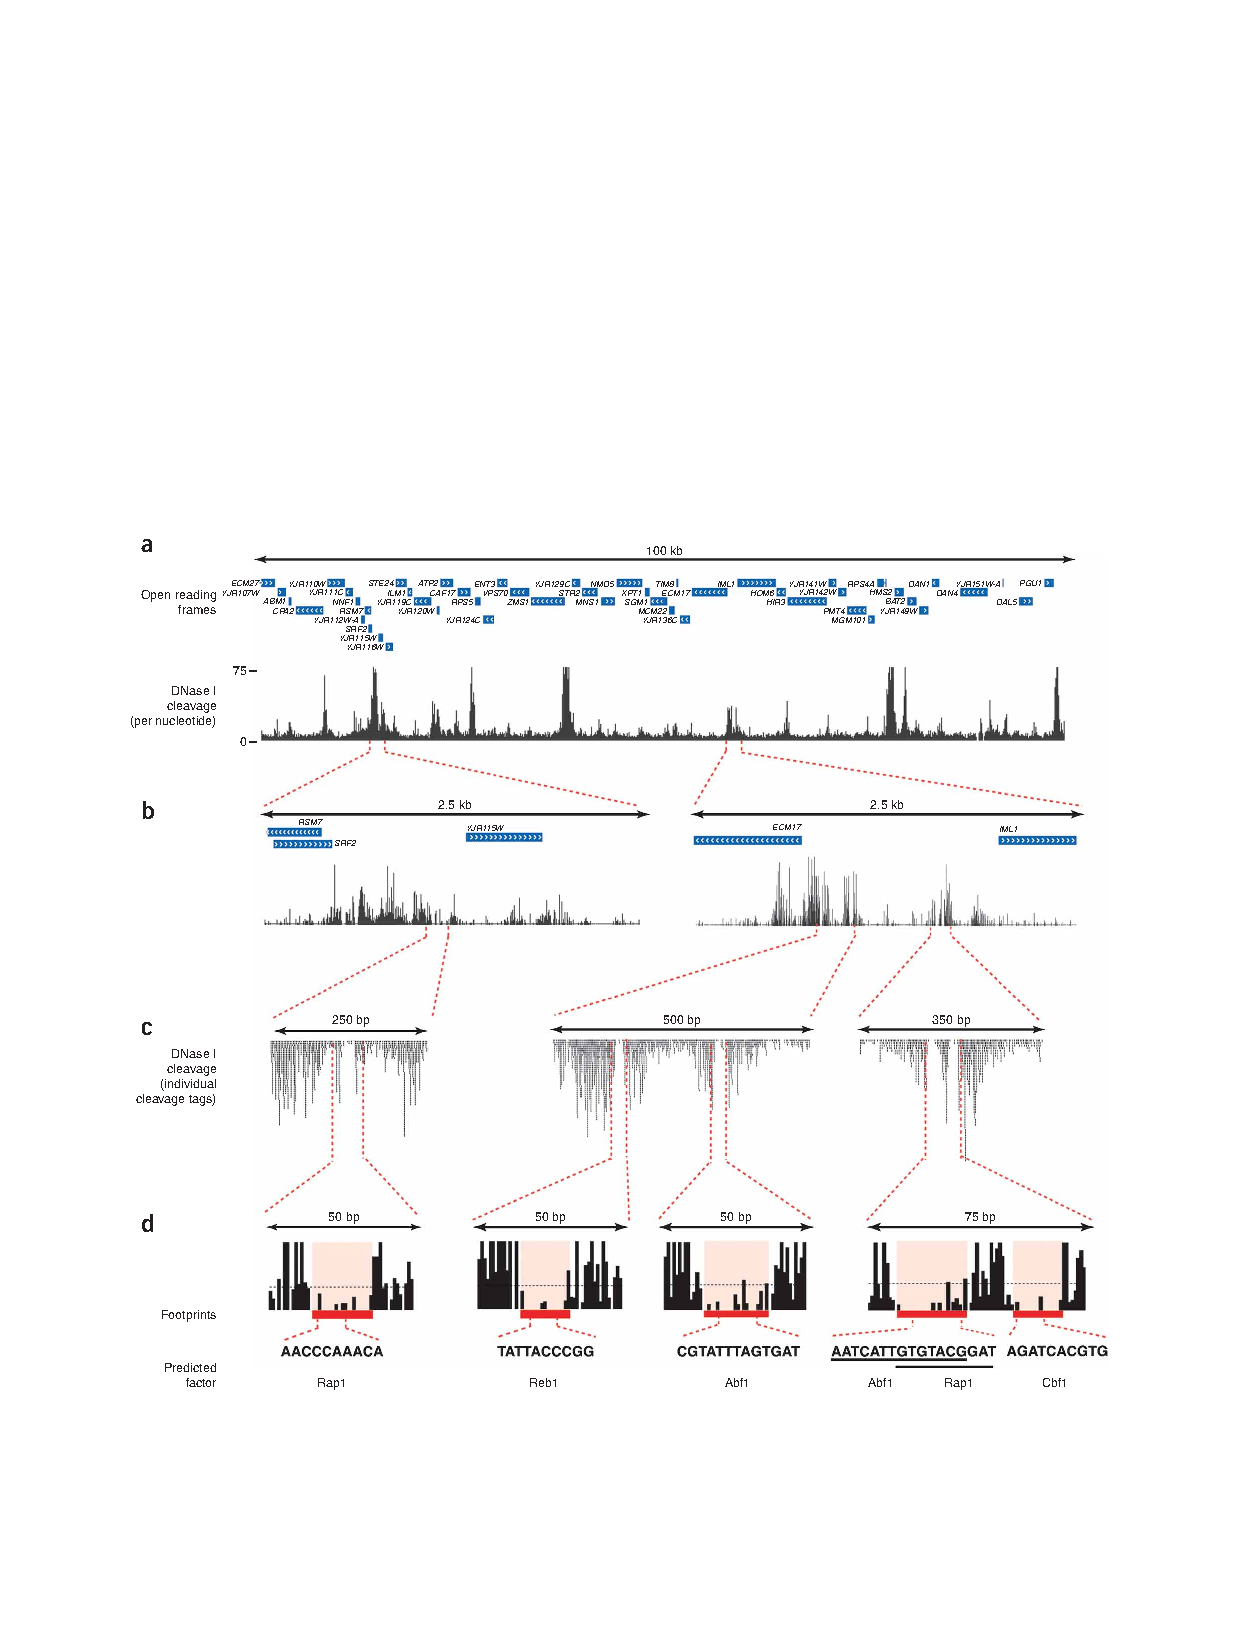
\includegraphics[width=\textwidth]{figures/hesselberth-dnase.pdf}
\captionbf{Exp�rience d'empreinte � la DNase I chez la levure : vers une r�solution au nucl�otide pr�s}{
Figure tir�e de \cite{Hesselberth2009vn}. (a) Densit� de digestion de la DNase
I par nucl�otide dans une r�gion de $100$kb du g�nome de la levure contenant
$\sim50$ g�nes (bo�tes bleues). On voit clairement certaines r�gions
promotrices marqu�es par la DNase I. (b) Zoom sur deux r�gions de $2.5$kb. (c)
Zoom sur des r�gions de $250$bp. Le nombre d'�v�nements de digestion par
nucl�otide est marqu� par des empilements de bo�tes noires, r�v�lant des
r�gions prot�g�es : ce sont les empreintes � la DNase I. (d) Les empreintes
sont associ�es � des motifs de r�gulation de la levure connus. Les pointill�s
noirs indiquent le nombre moyen de digestion par nucl�otide dans le g�nome
($\sim2$ digestions par base).
}
\label{fig:hesselberth-dnase}
\efigp

Contrairement aux techniques pr�c�dentes, l'empreinte � la DNase I ne repose
pas sur l'�tude d'un \tf pr�cis, mais permet au contraire d'obtenir l'ensemble
des sites de fixation dans le g�nome pour un type cellulaire donn�, avec une
pr�cision au nucl�otide pr�s. Cette m�thode repose sur le fait que la fixation
stable des \tfs � l'ADN n'est possible que si la r�gion est pauvre en
nucl�osomes, les prot�ines autour desquelles s'enroule l'ADN : on parle de
r�gion de chromatine ouverte. Ces r�gions sont pr�f�rentiellement dig�r�es par
l'endonucl�ase DNase I. �tant donn� que la majorit� de l'ADN est enroul� autour
de nucl�osomes, les sites hypersensibles � la digestion par DNase
I (\textit{DNase I-hypersensitive} ou DHS) correspondent essentiellement � des
r�gions de chromatine ouverte ayant des roles de r�gulation g�n�tique
: promoteurs, enhancers\ldots 
\\

En combinant la technique de DHS avec le s�quen�age � haut d�bit, l'exp�rience
de DNase-seq permet d'identifier tous les types de r�gion de r�gulation
� l'�chelle du g�nome~\cite{Thurman2012ys}. Les r�gions riches en sites de digestion
identifient alors les sites DHS. Par ailleurs, au sein d'un site DHS, il y a de
petites r�gions ($\sim15$bp) qui sont prot�g�es de la digestion par DNase
I : ce sont les empreintes � la DNase I ou \textit{DNase I footprints}
(fig.~\ref{fig:hesselberth-dnase}). Ces empreintes sont dues � la pr�sence de
prot�ines ou de complexes fix�s � l'ADN. Cette technique de d�tection de sites
de liaison par empreinte � la DNase I existe depuis $30$ ans mais n'a que
r�cemment �t� port� � l'�chelle g�nomique. En comparant � des donn�es \chipseq
ou en utilisant des bases de donn�es de motifs de \tfs, il est possible
d'identifier le facteur correspondant dont les sites de fixation sont alors
connus au nucl�otide pr�s.



\FloatBarrier
\section{Les modules de cis-r�gulation (CRMs)} \label{sec:CRMs} 
%
%\begin{malistebullet}{15}
%\item R�gulation transcriptionnelle. Facteurs de transcription. Diffusion, fixation. \\
%\item   Mod�les math�matiques (PWM, biophysiques). \\
%\item   Coop�rativit�, fonctions logiques, coefficients de Hill (Uri Alon).\\
%\item   Donn�es biologiques grande �chelle : \chipseq etc\ldots Bioinformatique.\\
%\item   ENCODE, Taipale, etc.\\
%\item   Evolution de la r�gulation Odom, Sinha.\\
%\end{malistebullet}

Nous l'avons vu en section \ref{sub:divers_modes_de_regulation}, les s�quences d'ADN
r�gulant l'expression g�n�tique -- CRMs pour \textit{Cis-Regulatory Modules} --
jouent un r�le pr�pond�rant au cours du d�veloppement des organismes. Ces CRMs
assurent en effet l'orchestration de l'expression de g�nes sp�cifiques aux
diff�rentes �tapes du d�veloppement et aux divers types cellulaires. Ils sont
au coeur de l'�volution des r�seaux g�n�tiques, car ils dictent les
interactions entre g�nes. De plus, leur alt�ration peut conduire � de
nombreuses pathologies, li�es pour la plupart � une expression g�n�tique
aberrante. Notamment, la majeure partie des variants g�n�tiques qui sont
associ�s de mani�re significative � une susceptibilit� envers une maladie sont
situ�s hors des r�gions codant pour des prot�ines, sugg�rant qu'un certain
nombre affectent non pas la forme de la prot�ine engendr�e mais l'expression du
g�ne la produisant en d�truisant une activit� CRM. Dans cette partie, nous
pr�sentons les diff�rents types de CRMs, leur structure, et leur �volution.

\subsection{Les diff�rents types de CRMs}
\label{sub:les_diff_rents_types_de_crms}

\bfig
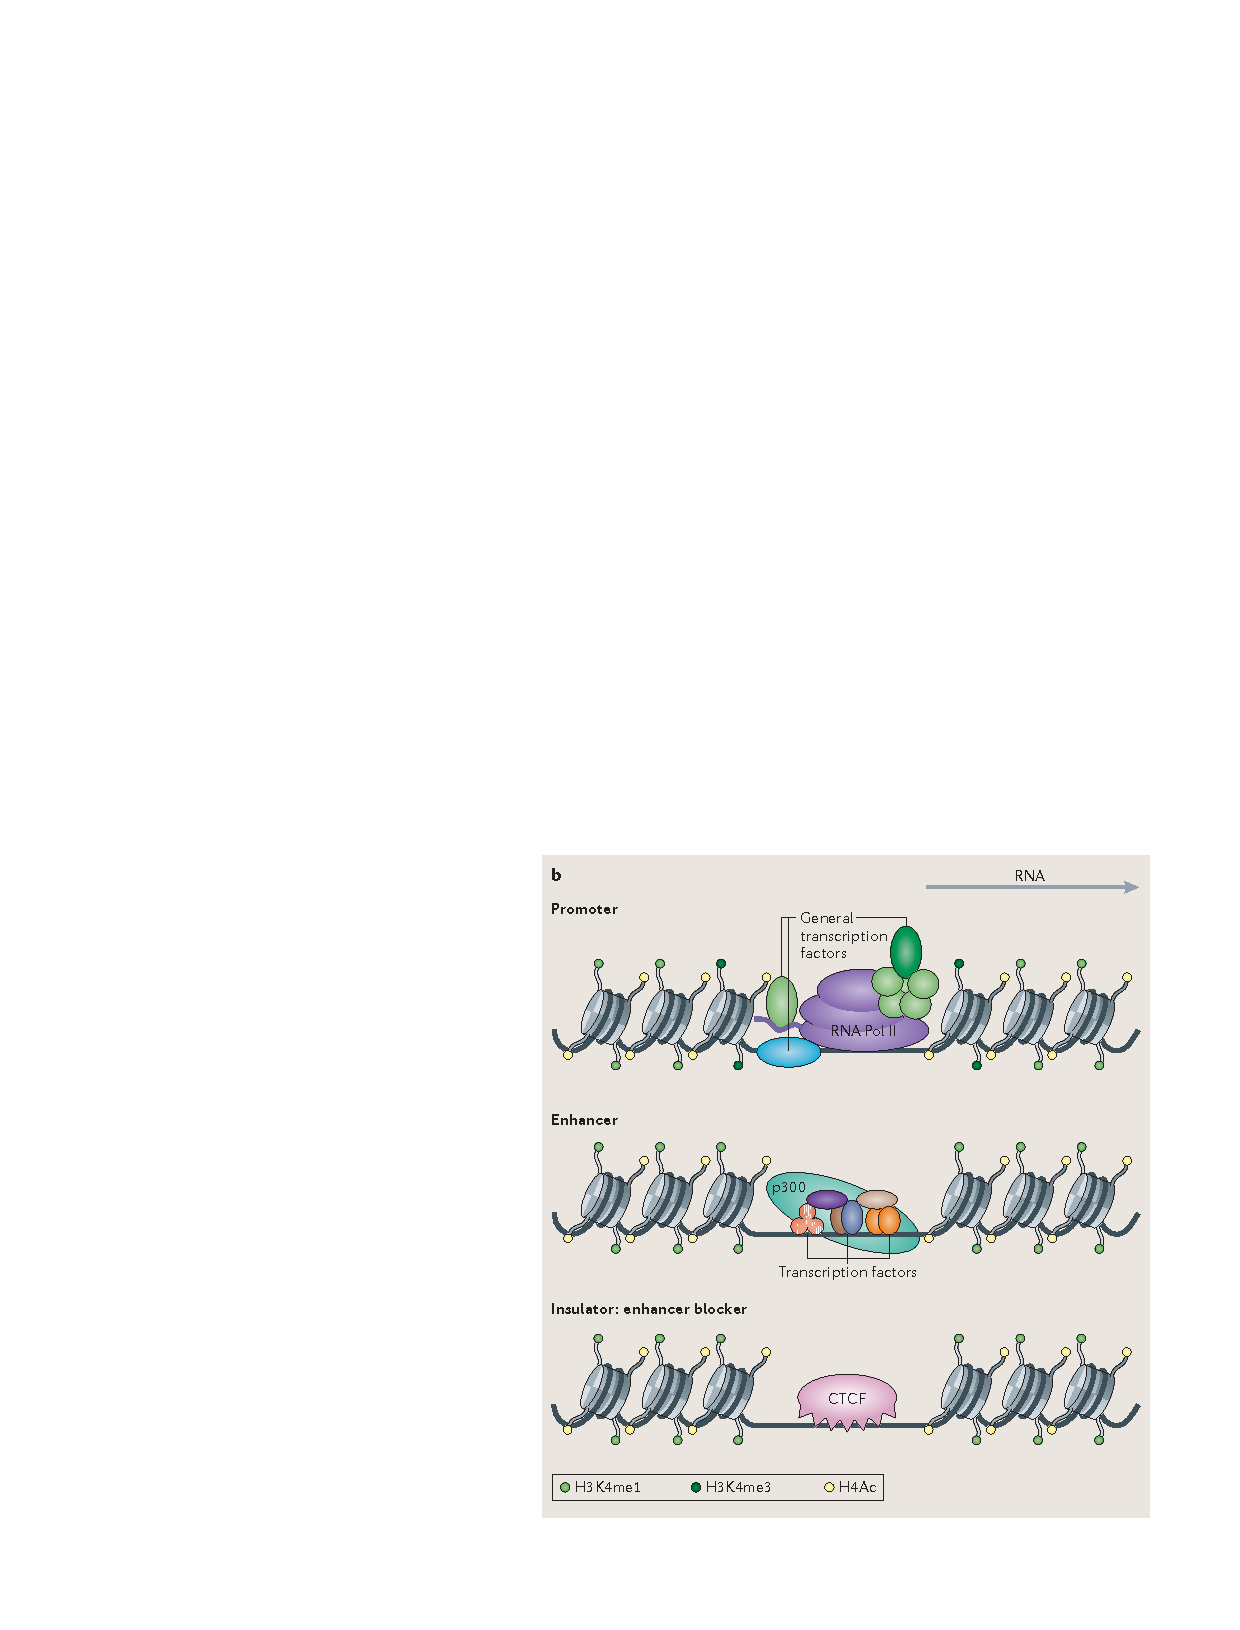
\includegraphics[width=1\textwidth]{figures/hardison-enhancer-states.pdf}
\captionbf{Les diff�rents types de CRMs et leurs marques �pig�n�tiques} 
{ 
    
    Figure tir�e de \cite{Hardison2012p3778}. La notion de CRM renvoie � un
    regroupement de sites de liaison pour un ou plusieurs \fts. Les CRMs
    peuvent �tre regroup�s en plusieurs classes : les promoteurs, les
    \textit{enhancers}/\textit{silencers}, et les insulateurs. Les CRMs des
    diff�rentes classes partagent les marques d'ac�tylation H3Ac et H4Ac, les
    promoteurs actifs sont sp�cifiquement marqu�s par H3K4me$3$, et les enhancers
    et insulateurs par H3K4me$1$. Les enhancers sont par ailleurs souvent
    fix�s par le co-activateur p$300$. Enfin, chez les mammif�res les insulateurs
    recrutent CTCF pour bloquer l'activation par les enhancers.

} 
\label{fig:hardison-enhancer-states}
\efig

Selon leur r�le dans la r�gulation de l'expression g�n�tique, les
CRMs peuvent �tre distingu�s en trois cat�gories.

\subsubsection{Promoteurs}
\label{ssub:promoteurs}

Les promoteurs permettent la fixation de l'ARN polym�rase pour d�buter la
formation d'un transcrit ARN au site d'initiation de transcription
(\textit{Transcription Start Site} ou TSS). Dans les promoteurs fixant l'ARN
polym�rase II (la majorit� des promoteurs eucaryotes), des \fts g�n�raux se
fixent � un coeur de $\sim100$bp autour du TSS afin de faciliter la fixation du
complexe de polym�rase. Ces coeurs de promoteurs contiennent pour certains des
motifs st�r�otyp�s, comme la bo�te TATA, et ont un TSS bien d�termin�;
n�anmoins la plupart des promoteurs des g�nomes mammif�res sont des r�gions
riches en GC et en dinucl�toides CpG (les \og �lots CpG \fg) qui ne poss�dent
pas de bo�te TATA et permettent l'initiation de la transcription dans un
interval d'environ $100$ bases~\cite{Carninci2006qf}. Au niveau �pig�n�tique,
les promoteurs actifs sont caract�ris�s par une r�gion pauvre en nucl�osomes en
amont du TSS, flanqu�e de nucl�osomes poss�dant la marque de m�thylation
H3K4me$3$.

% subsubsection promoteurs (end)

\subsubsection{\textit{Enhancers} et \textit{silencers}}
\label{ssub:enhancers_et_silencers}

Les \textit{enhancers} et \textit{silencers} sont respectivement d�finis par
leur effet positif ou n�gatif sur l'expression d'un g�ne cible. Cet effet peut
notamment �tre observ� par transfert d'un plasmide contenant l'�l�ment
r�gulateur en amont d'un g�ne rapporteur dans un animal transg�nique ou dans
des cultures cellulaires transfect�es (voir
\ref{sub:validation_experimentale}). Leur activit� ne d�pend g�n�ralement pas
de leur position et de leur orientation sur le plasmide. Selon l'environnement
cellulaire, une r�gion r�gulatrice peut �tre soit \textit{enhancer} soit
\textit{silencer}, en fonction de la nature de co-activateurs ou de
co-r�presseurs des TFs recrut�s. Il y a n�anmoins relativement peu de
\textit{silencers} caract�ris�s et l'on utilise le terme d'\textit{enhancers}
pour d�signer de mani�re g�n�rale ces r�gions r�gulatrices.

%\begin{figure}
\bfig
    \centering
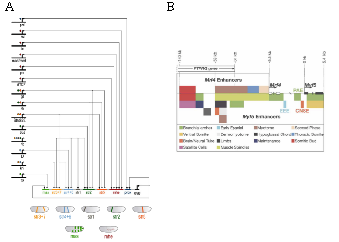
\includegraphics[width=1.0\textwidth]{figures/furlong-carvajal-enhancers-patterns.pdf}
\captionbf{Diff�rents \textit{enhancers} conduisent � diff�rents patterns d'expression}{
    
    (A) Figure tir�e de \cite{Wilczynski2010p575}, montrant le r�seau de
    cis-r�gulation du g�ne \textit{even-skipped} chez la \textit{Drosophile}.
    Des enhancers individuels (bo�tes color�es) conduisent � des motifs
    d'expression distincts (indiqu�s dans les embryons par la m�me couleur).
    Les cercles color�s au sein des r�gulateurs indiquent les couleurs des CRMs
    r�gul�s.

    (B) Figure tir�e de \cite{Carvajal2008p395}, repr�sentant les diff�rents
    �l�ments r�gulateur du locus \textit{Mrf4}/\textit{Myf5}. Chaque bo�te
    color�e repr�sente une r�gulation de la transcription � un stade de
    d�veloppement particulier ou dans une r�gion anatomique sp�cifique du
    muscle embryonnaire ou adulte.

} 
\label{fig:enhancers-pattern}
\efig
%\end{figure}

Les \textit{enhancers} peuvent se situer � des distances variables du g�ne
qu'ils r�gulent~\cite{Maniatis1987fk}, pouvant parfois aller jusqu'� $1$ Mb
comme dans le cas de \textit{Shh} chez la souris~\cite{Lettice2003uq} (voir
fig. \ref{fig:visel-shh-CRM-medical}). Les enhancers contiennent de multiples
sites de fixations de TFs. Cette multiplicit� est requise pour l'activit�
enhancer, comme cela l'a �t� montr� pour le premier enhancer d�couvert : celui
du virus simien 40 (SV40)~\cite{Schirm1987kx,Ondek1988vn}. Un g�ne peut par
ailleurs poss�der plusieurs enhancers distincts conduisant � des expressions
sp�cifiques dans diff�rents tissus, comme cela l'a �t� montr� dans le cas du g�ne
\textit{eve} chez la \textit{Drosophile}~\cite{Wilson2009p3225} ou dans le cas
du cluster de g�nes de d�termination myog�nique \textit{Myf5} et \textit{Mrf4}
chez les mammif�res~\cite{Carvajal2008p395} (fig.~\ref{fig:enhancers-pattern}).
Ainsi, les diff�rents enhancers d'un m�me g�ne peuvent �tre vus comme autant de
points d'entr�e d'un r�seau de r�gulation g�n�tique, repr�sentant diverses
fonctions logiques et int�grant diff�rentes information spatio-temporelles pour
produire en sortie une expression g�n�tique spatio-temporelle finement
contr�l�e~\cite{Bolouri2002uq,Buchler2003fu}.

Enfin, comme d�crit en fig.~\ref{fig:hardison-enhancer-states}, les enhancers
sont associ�s � de hauts niveaux de marque �pig�n�tique
H3K4me$1$~\cite{Heintzman2009ys} et sont souvent fix�s par le co-activateur
p$300$~\cite{Wang2005zr,Heintzman2009ys}.


\subsubsection{Insulateurs}
\label{ssub:insulateurs}

Les insulateurs sont des CRMs qui restreignent l'effet des enhancers sur leur
g�ne cible~\cite{Wallace2007ly}. Ainsi, certains insulateurs poss�dent une
activit� de blocage d'enhancers. Situ�s entre un enhancer et un promoteur
cible, ces insulateurs bloquent l'activit� de l'enhancer, conduisant � une
r�duction de l'expression du g�ne cible~\cite{Chung1993ve}. Chez les
mammif�res, la fixation de la prot�ine CTCF est n�cessaire � cette activit� de
blocage de l'activit� enhancer~\cite{Bell1999qf}, alors que chez la
\textit{Drosophile} et plusieurs autres insectes il existe au moins quatre
prot�ines additionnelles qui sont suffisantes � la r�alisation de cette
activit�~\cite{Schoborg2010bh}. Par ailleurs, les insulateurs peuvent
servir de barri�re de protection contre des marques d'h�t�rochromatine
r�pressives. De tels insulateurs permettent notamment d'�viter les
effets de positions -- la modification de l'expression d'un g�ne selon sa
position dans le chromosome -- lorsqu'ils entourent un g�ne rapporteur int�gr�
au hasard dans le g�nome~\cite{Recillas-Targa2002dq}. Cette activit� passe
notamment par le recrutement de \textit{USF}, prot�ine qui recrute des enzymes
de modification de la chromatine. Un insulateur peut combiner les activit�s de barri�re de protection et de blocage d'enhancer.

De m�me que les enhancers, les insulateurs peuvent se situer � des distances
variables des g�nes qu'ils r�gulent. Il est � noter que la prot�ine CTCF
poss�de d'autres fonctions que celle d'isolation, et tous les sites de CTCF ne
correspondent pas forc�ment � des insulateurs~\cite{Phillips2009cr}.

% subsubsection insulateurs (end)

% subsubsection enhancers_et_silencers (end)

% subsection les_diff_rents_types_de_crms (end)

%\subsection{Modules et fonctions logiques}

%\bfig
%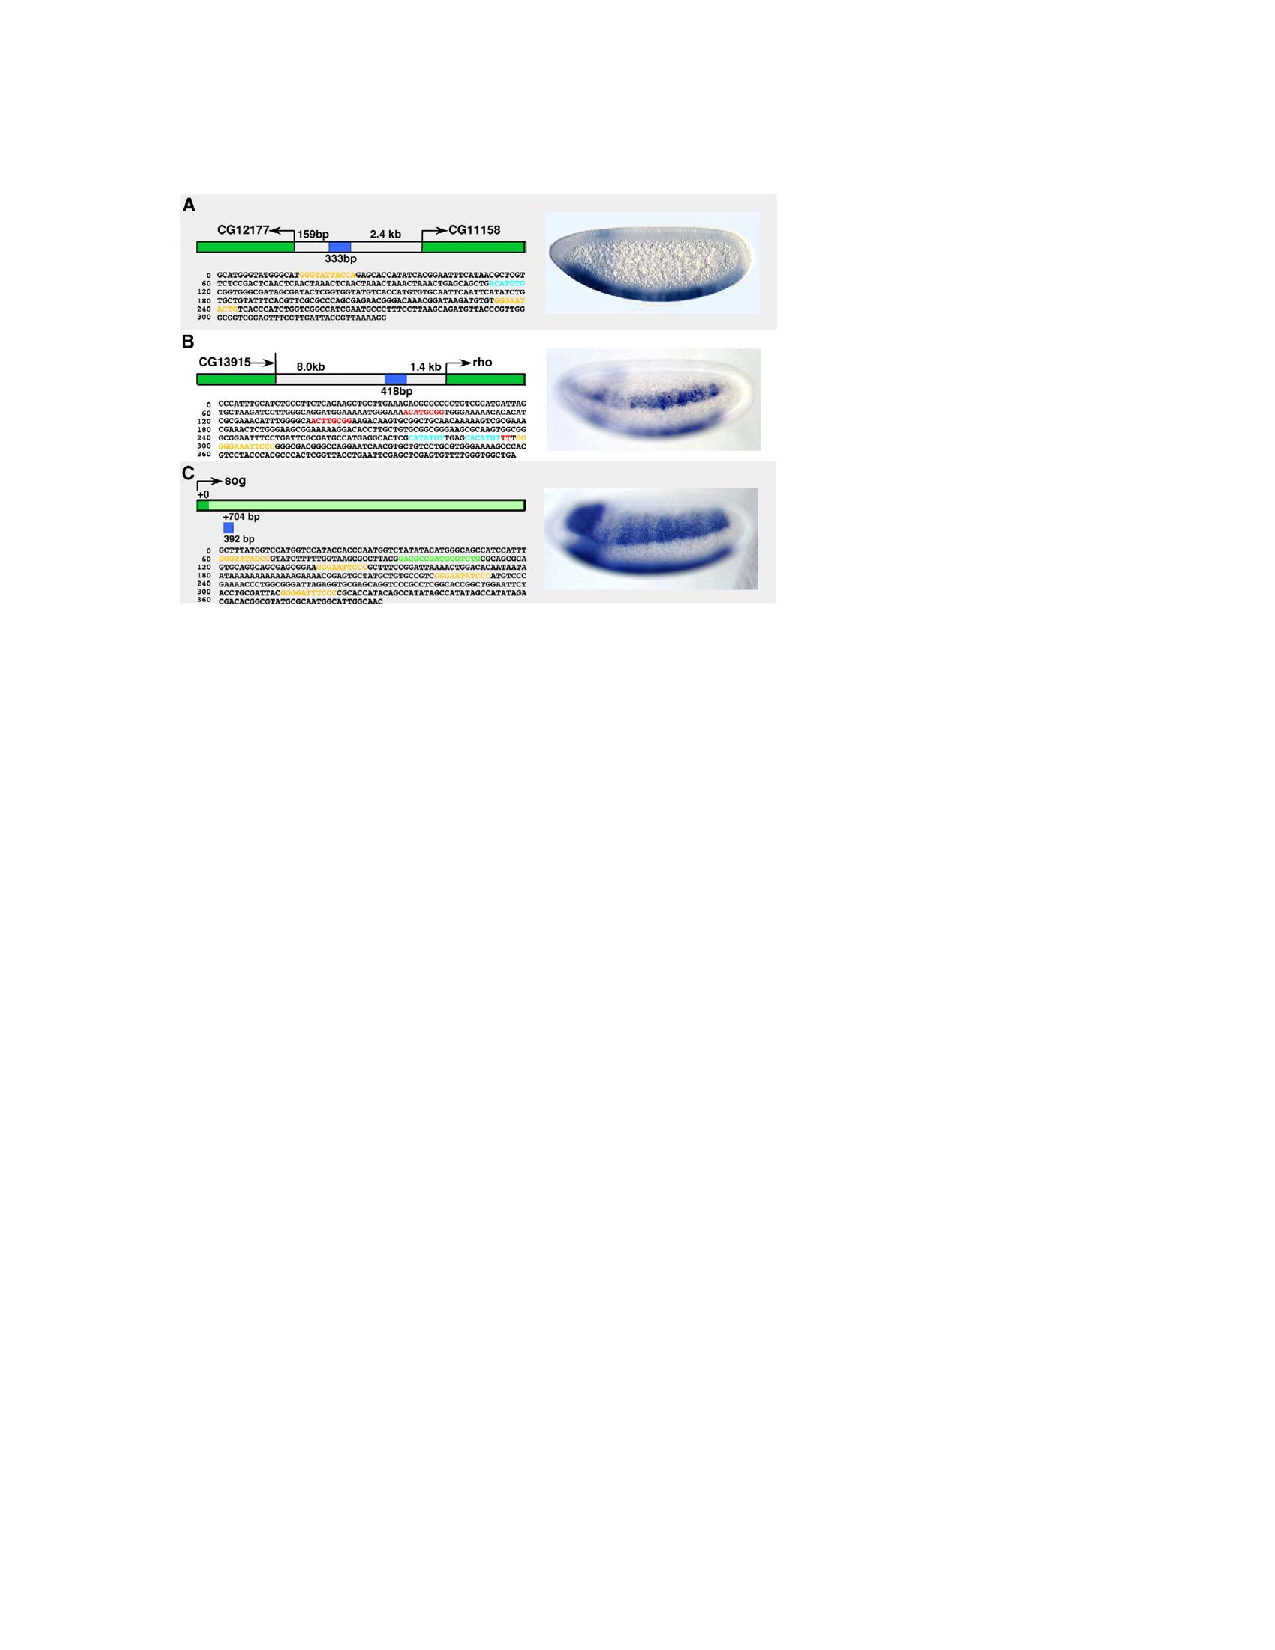
\includegraphics[width=\textwidth]{figures/stathopoulos-CRMs-sites-twist-dorsal-snail.pdf}
%\captionbf{}{
    %Figure tir�e de \cite{Stathopoulos2005p4051}.
%} 
%\efig

\subsection{Grammaire des enhancers : enhanceosome vs billboard}
\label{sub:enhanceosome_billboard}

\begin{figure}[p!]
    \centering
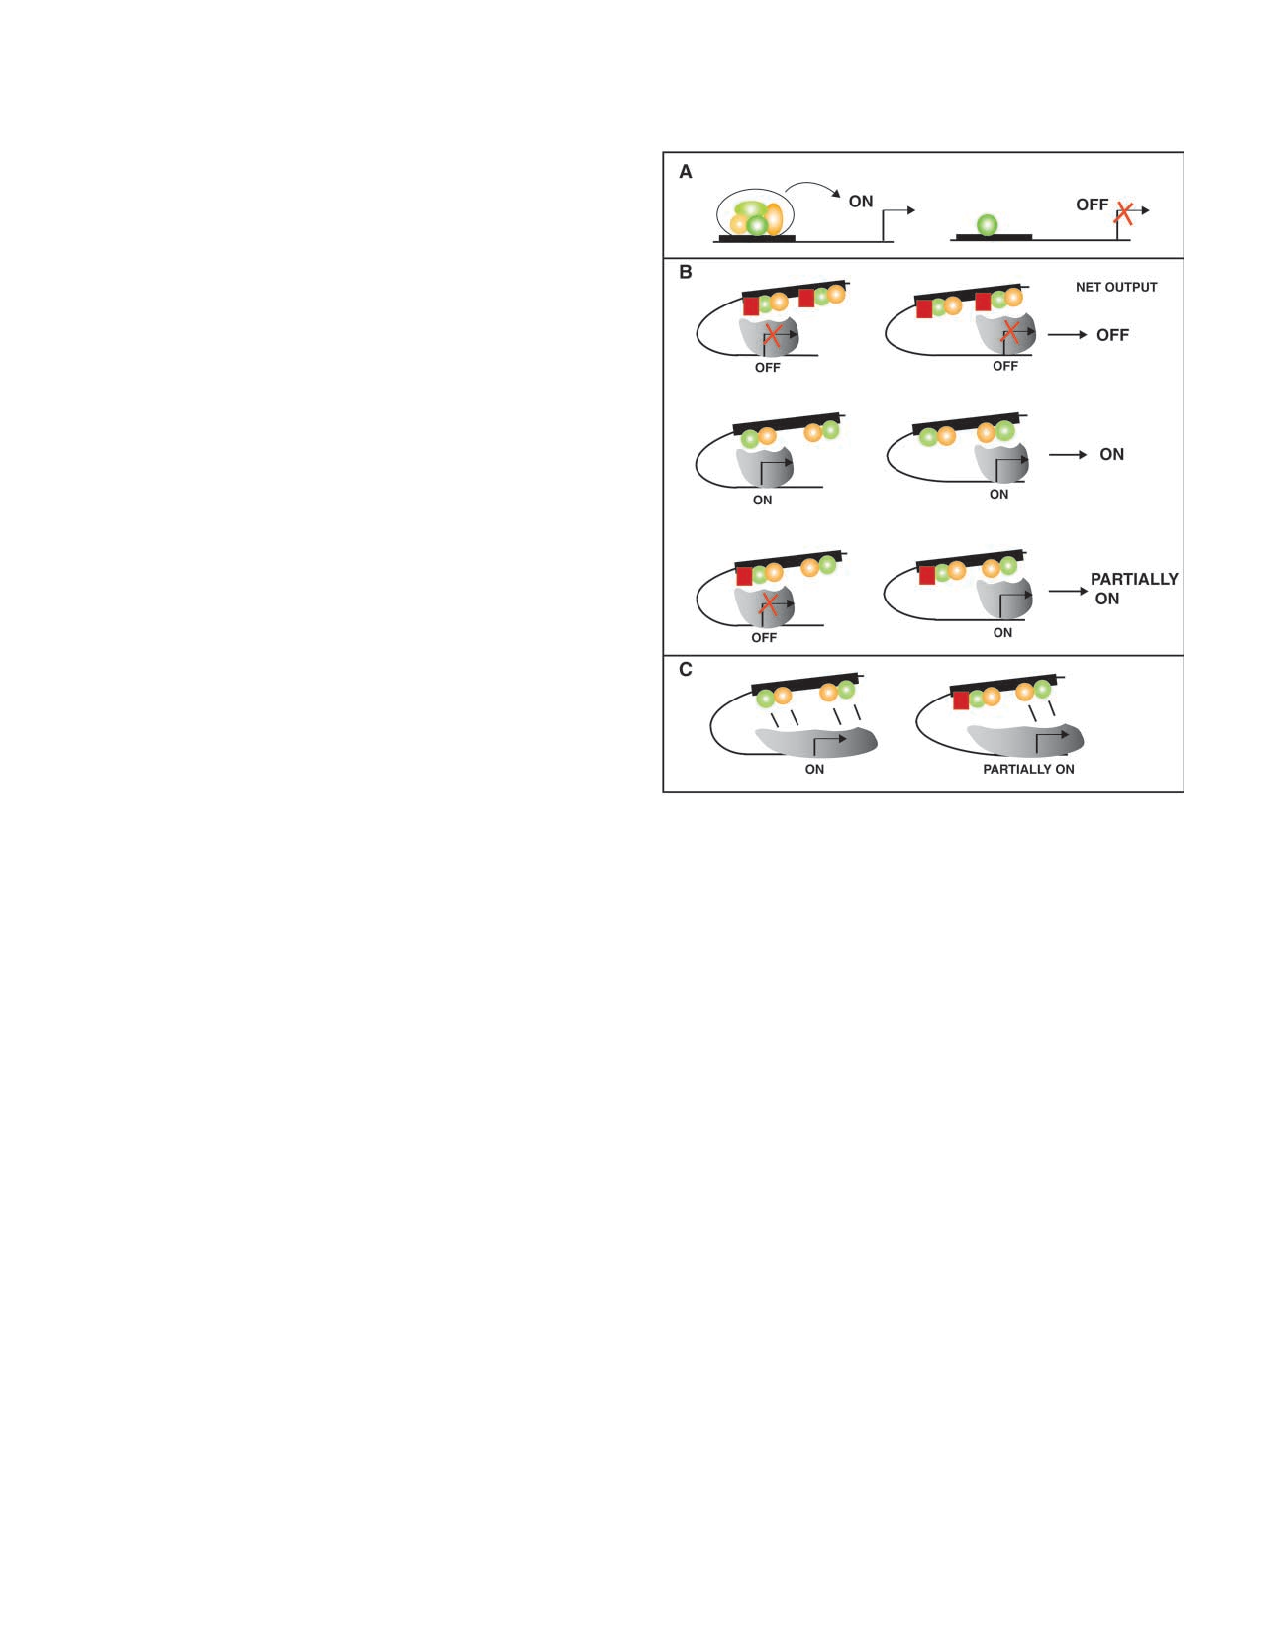
\includegraphics[width=.8\textwidth]{figures/kulkarni-billboard.pdf}
\captionbf{Deux mod�les d'enhancers: enhanceosome et billboard}{

    Figure tir�e de~\cite{Kulkarni2003nx}. (A) Dans le mod�le enhanceosome,
    l'enhancer traite l'information des multiples TFs qui le fixent. Un
    complexe tr�s structur� cr�e une interface qui recrute la
    machinerie de transcription basale. L'enhancer peut �tre vu comme un
    ordinateur mol�culaire qui produit � partir d'entr�es multiples un seul
    signal vers la machinerie de transcription. Le g�ne cible n'est activ�
    qu'en cas de formation du complexe entier, ce qui fournit un interrupteur
    binaire on/off seulement activ� en cas de stimulus ad�quat. La
    d�stabilisation du complexe en changeant par exemple la concentration d'une
    des prot�ines permettrait alors d'obtenir une r�ponse graduelle.  (B,C)
    Mod�le d'enhancer \og billboard \fg. Dans ce cas, l'enhancer ne consiste pas en
    une seule unit� de r�gulation, mais en des sous-unit�s pouvant contenir
    diff�rentes informations (r�pression ou activation par exemple) que la
    machinerie basale �chantillonne soit it�rativement (B), soit simultan�ment
    (C).

} 
\label{fig:kulkarni-billboard}
\end{figure}


Nous l'avons vu, les CRMs contiennent en g�n�ral de multiples sites de liaisons
(TFBS) pour un ou plusieurs TFs. On parle de \textit{clustering}
(regroupement). Lorsque les TFBS correspondent � plusieurs TFs diff�rents, on
parle de CRM h�t�rotypique, et dans le cas o� ils correspondent � un m�me TF,
on parle de CRM homotypique. Cette distinction est surtout utile pour d�crire
les diff�rentes m�thodes de pr�diction de CRM, car la plupart des CRMs
identifi�s chez les M�tazoaires sont h�t�rotypiques~\cite{Aerts2012p3868}.
L'organisation de ces sites de liaison rel�ve de deux types d'architecture
principaux (fig.~\ref{fig:kulkarni-billboard}).


\bfig

\includegraphics[width=0.8\textwidth]{figures/panne-enhanceosome.pdf}
\captionbf{L'enhanceosome de l'interferon-$\beta$}{

    Figure tir�e de~\cite{Panne2008kl} repr�sentant le complexe de TFs
    assembl�s sur l'enhanceosome IFN-$\beta$, formant une surface de
    reconnaissance agissant comme une seule unit� de r�gulation.

}
\label{fig:panne-enhanceosome}
\efig

\subsubsection{Le mod�le ``enhanceosome''}
\label{ssub:le_mod_le_enhanceosome_}

Dans ce mod�le, l'architecture des sites de liaison est de premi�re importance. Le
paradigme en est l'enhancer du g�ne humain interferon-$\beta$, sur lequel $8$
TFs se lient pour former une surface de reconnaissance
continue~\cite{Panne2008kl}. Les TFBS de cet enhancer se recouvrent les uns les
autres, cr�ant au final un complexe de TFs fix�s � l'ADN agissant comme une
seule unit� de r�gulation (fig.~\ref{fig:panne-enhanceosome}).


% subsubsection le_mod_le_enhanceosome_ (end)


\subsubsection{Le mod�le ``billboard''}
\label{ssub:le_mod_le_billboard_}

La majorit� des CRMs adh�rent � ce type d'organisation. L'architecture y est
libre : les sites de liaisons n'ont pas de contrainte de nombre, d'ordre, de
sens, ou d'espacement~\cite{Kulkarni2003nx}. De tels CRMs sont propices � une
d�tection informatique bas�e sur la densit� en sites de liaisons pour
diff�rents TFs.

% subsubsection le_mod_le_billboard_ (end)



\subsection{�volution des enhancers}
\label{sub:evolution-des-enhancer}

La fonction centrale que jouent les enhancers dans la r�gulation de
l'expression g�n�tique laisse � penser que ceux-ci seraient sous s�lection et
leur s�quence serait donc plus conserv�e que celle des r�gions non codantes du
g�nome. De fait, la comparaison de s�quences non-codantes entre esp�ces proches
s'av�re �tre un mode de d�tection puissant des r�gions de
r�gulation~\cite{Prabhakar2006ys}. Ainsi, l'utilisation de la conservation
entre des esp�ces lointaines comme l'homme et le poisson \textit{Fugu} ou de
l'extr�me conservation entre des esp�ces proches comme l'homme, la souris et le
rat, permet de d�tecter des r�gions ayant une activit� enhancer \invivo avec un
succ�s proche de $50\%$~\cite{Pennacchio2006vn}. � l'instar de la r�gulation de
l'interf�ron-$\beta$, de telles s�quences tr�s contraintes ob�issent � une
logique de type \og enhanceosome \fg o� la fonction est intimement li�e � la
s�quence.



\bfigp
\includegraphics[width=0.95\textwidth]{figures/liberman-crm-conservation-flexibility.pdf}
\captionbf{Flexibilit� du code de cis-r�gulation au cours de l'�volution chez les \textit{Drosophiles}}{

    Figure tir�e de \cite{liberman2009p3886}, montrant l'expression du g�ne
    \textit{sog} par ISH chez plusieurs esp�ces de \textit{Drosophilid\ae}
    (A,D,G,J), ainsi que l'expression d'un rapporteur \textit{LacZ} sous
    contr�le de la r�gion de r�gulation de \textit{sog} chez l'esp�ce
    consid�r�e (B,E,H,K), dont une repr�sentation sch�matique est donn�e pour
    chaque cas (C,F,I,L).  Les sites de fixation pour diff�rents TFs sont
    indiqu�s par un rectangle de couleur.

} 
\label{fig:liberman-crm-flexibility}
\efigp


Contrastant avec cette vision d'enhancers tr�s contraints, plusieurs �tudes
pointent vers une plus grande flexibilit� des s�quences
enhancers~\cite{Ludwig2000zr,Dermitzakis2002ly,Moses2006ve}. Supportant l'id�e
que la plupart des enhancers se comportent selon le mod�le \og billboard \fg,
la grammaire des sites de fixation dans des s�quences orthologues appara�t
comme �tant loin d'�tre fig�e~\cite{liberman2009p3886}. Ainsi, l'enhancer
r�gulant le g�ne \textit{short gastrulation} (\textit{sog}), bien que
pr�sentant chez diff�rentes esp�ces de \textit{Drosophiles} une architecture
variable des sites de fixation le composant, conduit � un m�me motif
d'expression (fig.~\ref{fig:liberman-crm-flexibility}). Cette id�e qu'une
panoplie de grammaires conduisent � une m�me r�gulation est confort�e par les
r�sultats de~\citet{Zinzen2009p760} o� des enhancers ayant des \og entr�es \fg
diff�rentes (i.e �tant fix�s par des TFs diff�rents pendant des dur�es
variables) produisent des \og sorties \fg similaires, dans ce cas une
expression sp�cifique � un tissu donn�.  


Supportant l'id�e d'une flexibilit� de la r�gulation, plusieurs �tudes ont
exhib� l'�volution rapide des sites de liaison de TFs dans le
g�nome~\cite{Wilson2009p3225}. Une �tude de la fixation g�nomique des \tfs
CEBP$\alpha$ et HNF4$\alpha$ dans les cellules du foie de $5$ esp�ces de
vert�br�s (l'homme, deux esp�ces de souris, le chien et le poulet) a notamment
montr� que les �v�nements de fixation conserv�s chez les $5$ esp�ces sont tr�s
rares ($\sim0.3\%$ des pics humains) et correspondent � des r�gions
ultraconserv�es proches de g�nes importants dans la sp�cification du
foie~\cite{Schmidt2010p3228}. Par ailleurs, lors de la perte de fixation dans
l'une des esp�ce, un gain de fixation proche ($\pm10$kb) est observ� dans la
moiti� des cas. �tonnamment, ces changements rapides du c�blage du r�seau
affectent peu l'expression g�n�tique globale~\cite{Tirosh2008qf,Odom2007bh}.

Cette �volution est en grande partie due � une �volution de s�quence de
fixation. Ainsi, une �tude r�cente a utilis� une souris portant le chromosome
$21$ de l'homme pour comparer la fixation du facteur HNF4$\alpha$ dans un
contexte murin par rapport au contexte original~\cite{Wilson2008dq}. Le paysage
de fixation sur le chromosome $21$ exog�ne a tr�s pr�cis�ment r�capitul� celui
observ� chez l'homme (fig.~\ref{fig:wilson-CRMs-evolution}), montrant que le
contexte cellulaire est sensiblement le m�me chez les deux esp�ces. Par
ailleurs, des modifications �pig�n�tiques ainsi que l'expression des ARNm ont
pu �tre r�capitul�es.

\bfigp
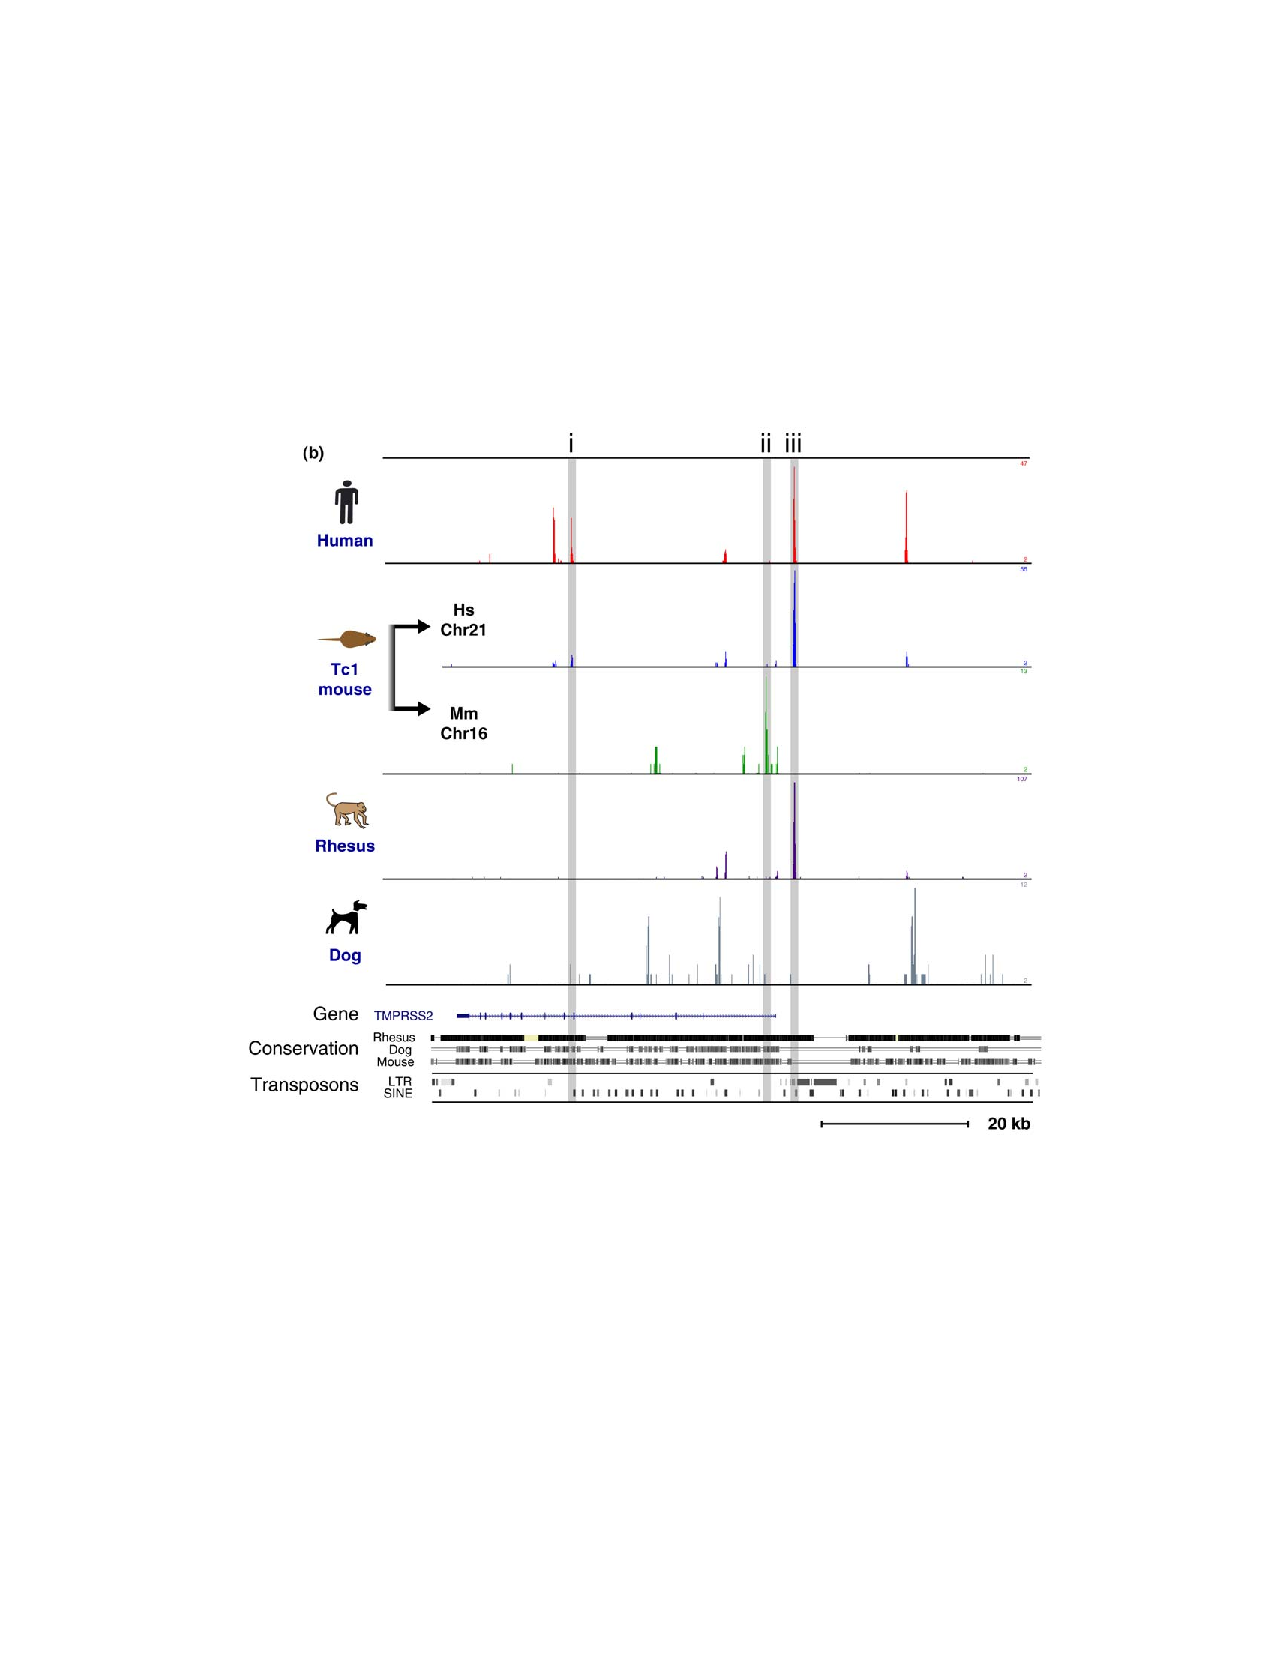
\includegraphics[width=1\textwidth]{figures/wilson-CRMs-evolution.pdf}
\captionbf{�volution de la fixation de HNF$4\alpha$ chez les mammif�res}{
    
    Figure tir�e de \cite{Wilson2009p3225}, repr�sentant la fixation par
    \chipseq (pics de couleur) du facteur de transcription humain HNF$4\alpha$
    (ou son homologue murin HNF$4$a) chez l'homme, la souris, le macaque, le
    chien, ainsi qu'une souris transg�nique contenant le chromosome 21 humain.
    Les zones gris�es indiquent : (i) une fixation de HNF$4\alpha$ chez l'homme
    retrouv�e sur le chromosome 21 humain de la souris mais pas chez le macaque
    malgr� la proximit� de s�quence, (ii) une fixation de HNF$4$a sp�cifique
    � la souris, et (iii) une fixation sp�cifique aux primates qui a lieu sur
    des �l�ments transposables. 

} 
\label{fig:wilson-CRMs-evolution}
\efigp


Reste la question du m�canisme permettant cette �volution rapide. Une �tude
portant sur $7$ \tfs chez les mammif�res a montr� qu'une proportion
importante ($\sim20\%$) des r�gions de fixation de ces TFs se situent au
sein de diff�rentes familles de transposons~\cite{Bourque2008p3218}
(fig.~\ref{fig:wilson-CRMs-evolution}). Ces transposons, ou �l�ments
transposables, sont des anciens r�trovirus int�gr�s dans les g�nomes mammif�res
ayant la capacit� de se dupliquer pour s'int�grer dans une autre r�gion du
g�nome et jouent un r�le fondamental dans l'�volution des
g�nomes~\cite{Cordaux2009p1515}. Leur accumulation dans le g�nome
a vraisemblablement permis d'obtenir un mat�riau de base permettant de produire
par mutations ponctuelles des �l�ments de r�gulation \textit{de
novo}~\cite{Feschotte2008dq}. Par ailleurs, les transposons peuvent permettre
de diffuser par \og copier-coller \fg des �l�ments de r�gulation existant.
Ainsi, des vagues d'expansion de transposons sp�cifiques � diff�rentes esp�ces
de mammif�res sont � l'origine de la variabilit� des r�gions de fixation
observ�e dans le cas du facteur CTCF~\cite{Schmidt2012p3262}.

\subsection{Les \og shadow enhancers \fg}
\label{sub:shadow_enhancers}


L'�volution des �l�ments de cis-r�gulation est un m�canisme majeur permettant
la diversit� animale. N�anmoins, de tels changements pourraient compromettre
certaines activit�s g�n�tiques essentielles. Des exp�riences de
\chipchip ont sugg�r� que plusieurs g�nes de d�veloppement actifs lors du
d�veloppement pr�coce de l'embryon de Drosophile poss�dent des CRMs
secondaires, qui conduisent � des motifs d'expression g�n�tique comparables
� ceux produits par des CRMs \og primaires \fg plus
proximaux~\cite{Zeitlinger2007ly}. L'expression de \og shadow enhancer \fg
a �t� propos�e par Michael Levine en 2008 pour d�crire ces CRMs redondants et
souvent distaux de plusieurs dizaines de kb du g�ne r�gul�~\cite{Hong2008zr}.
Il est probable que de tels CRMs soient apparus au cours de l'�volution par
duplication du CRM primaire, � l'instar du ph�nom�ne de duplication des
s�quences codant pour des prot�ines.  L'avantage �vident que peut conf�rer la
redondance d'un �l�ment de r�gulation est d'offrir de la robustesse face aux
mutations. Par ailleurs, une telle redondance permet de faciliter la divergence
et donc la sp�cialisation des diff�rents CRMs. Ainsi les \se semblent �voluer
plus rapidement que les CRMs primaires auxquels ils sont
apparent�s~\cite{Hong2008zr} pour fournir de nouveaux sites de fixation et
conduire � de nouvelles activit�s de r�gulation sans bloquer la fonction
critique de certains g�nes de d�veloppement.

\bfig
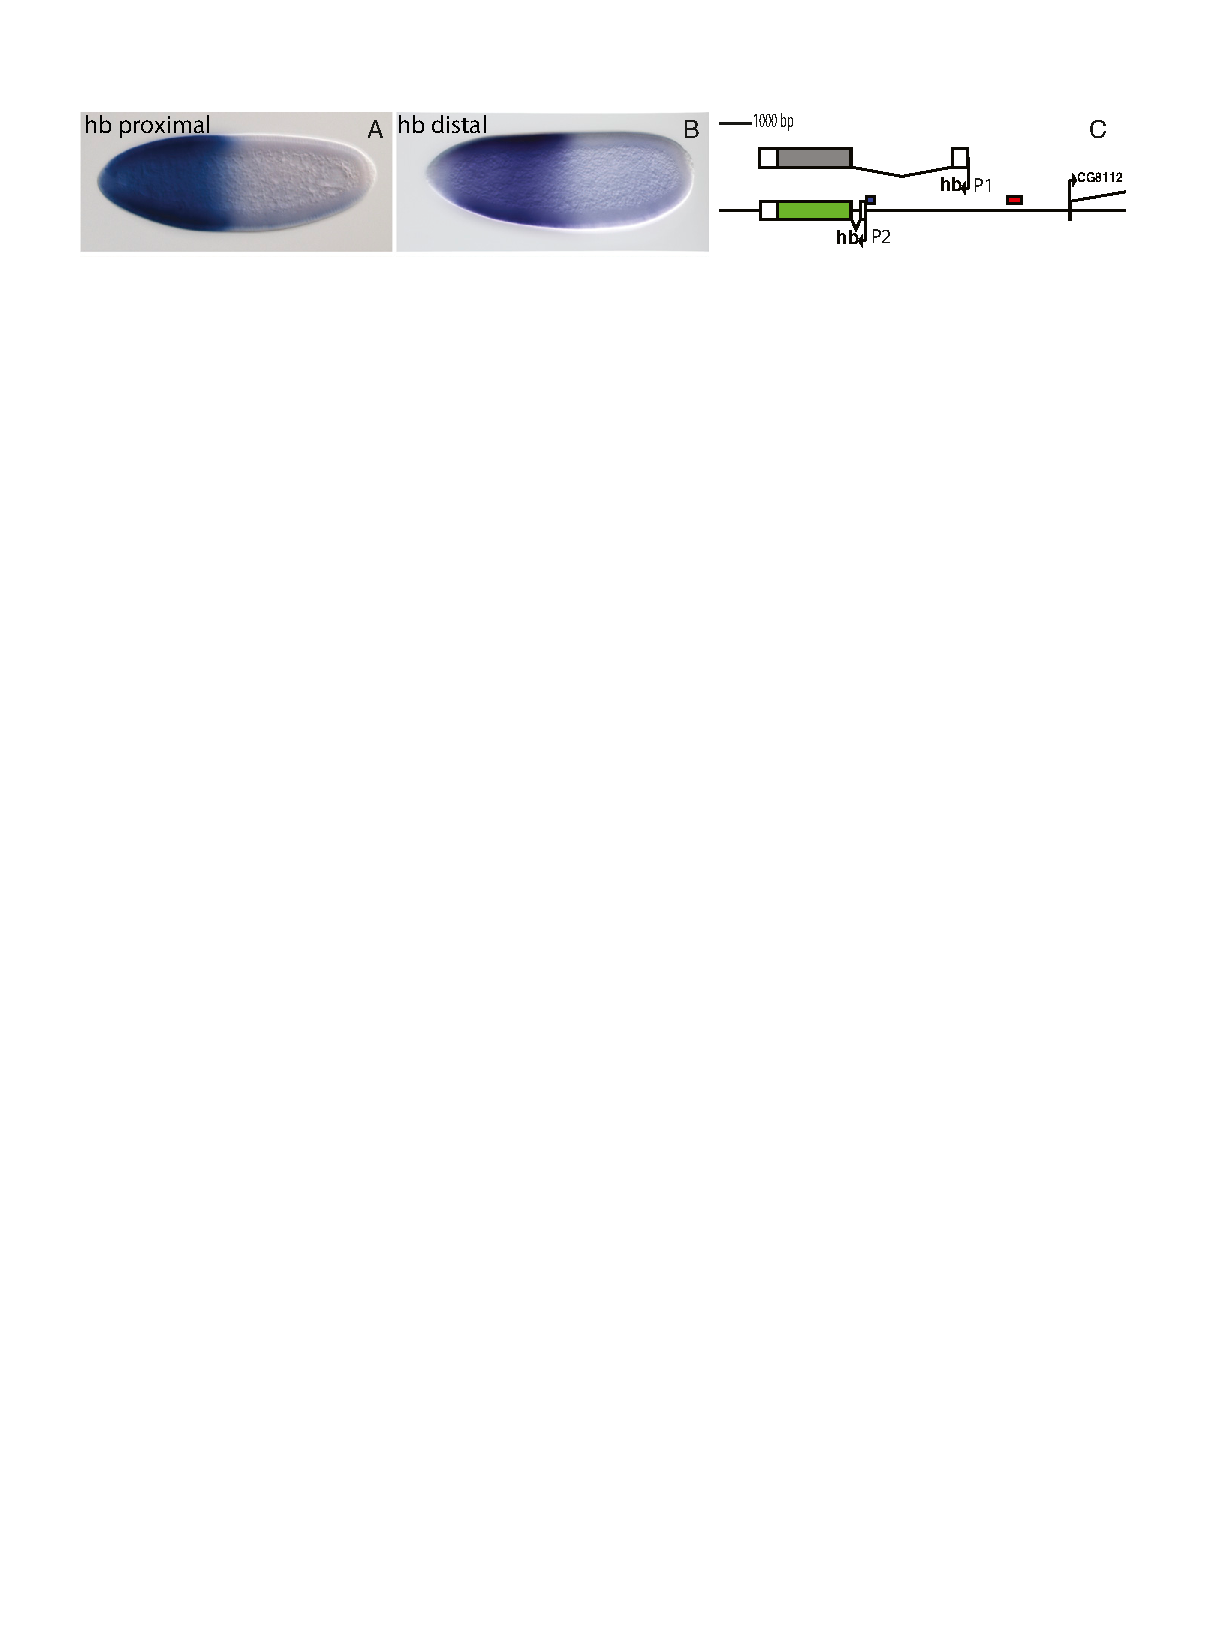
\includegraphics[width=1.0\textwidth]{figures/perry-shadow-enhancer.pdf}
\captionbf{\og Shadow enhancer \fg du g�ne de segmentation \textit{Hunchback}}{
    
    Figure tir�e de~\cite{Perry2011ve}, montrant des hybdridations \insitu de
    transg�nes contenant le g�ne rapporteur \textit{LacZ} sous contr�le de
    l'enhancer proximal (A) ou du \og shadow enhancer \fg plus distal (B) du
    g�ne de segmentation \textit{Hb}. (C) Position des enhancers par rapport
    � \textit{Hb} (bleu : proximal, rouge : distal). 

}
\label{fig:perry-shadow-enhancer}
\efig

Un exemple m�lant robustesse et divergence est le
cas des multiples CRMs r�gulant le g�ne \textit{Svb} chez la Drosophile.
Chaque CRM est li� � la production d'un motif distinct de trichomes
(excroissances de l'�pith�lium comparables � des poils) sur la larve : ainsi,
plusieurs mutations dans ces diff�rents CRMs sont n�cessaires pour observer un
changement morphologique cons�quent~\cite{McGregor2007p400}. Dans ce m�me
syst�me, il a �t� montr� que deux CRMs suppl�mentaires, des \se, sont
dispensables dans des conditions de temp�rature usuelles, mais requis lorsque
les embryons se d�veloppent dans des conditions de temp�rature
extr�mes~\cite{Frankel2010p463}.


Par ailleurs, il a �t� montr� que les g�nes de segmentation (ou g�nes
\textit{gap}) de la Drosophile poss�dent tous des \se
(fig.~\ref{fig:perry-shadow-enhancer}). Leur r�le semble �tre d'assurer une
plus grande pr�cision spatiale du motif d'expression du g�ne
r�gul� : la perte de l'un des CRMs, proximal aussi bien que
\og shadow \fg, conduisant � une expression trop restreinte ou trop r�pandue
spatialement selon le cas~\cite{Perry2011ve}.


\subsection{Par del� les enhancers: les \og super-enhancers \fg}
\label{sub:les_super_enhancers}


\bfig
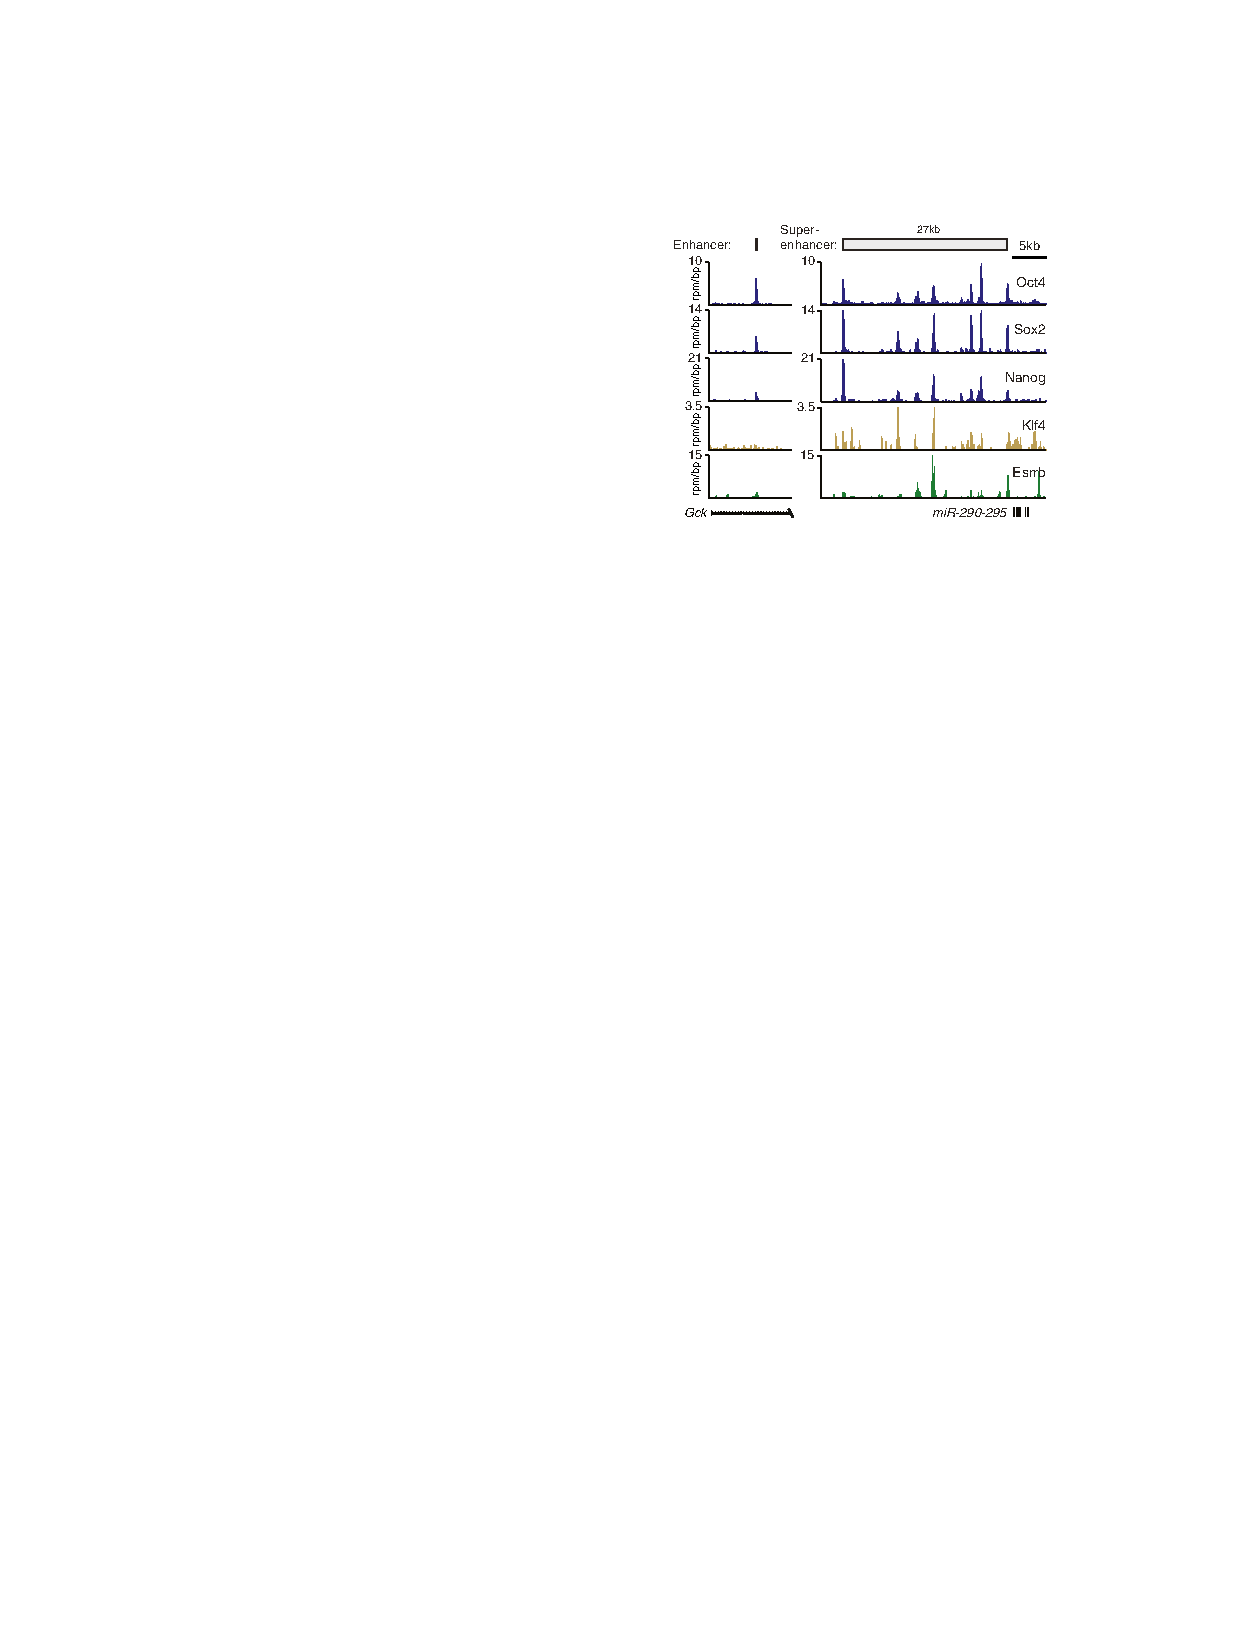
\includegraphics[width=0.8\textwidth]{figures/whyte-super-enhancer-cluster.pdf}
\captionbf{De l'enhancer au super-enhancer}{

    Figure tir�e de~\cite{Whyte2013tg}, montrant les profils de \chipseq des
    TFs ma�tres Oct4, Sox2, Nanog, Klf4 et Esrrb aux loci de \textit{Gck} et
    \textit{miR-290-295} dans les cellules souches embryonnaires. Le
    super-enhancer se distingue du simple enhancer par sa taille ($27$kb), sa
    grande concentration en TFs ma�tres, notamment Klf4 et Esrrb, et la
    fixation de la prot�ine Med$1$ du complexe Mediator.

}
\label{fig:whyte-super-enhancer}
\efig

R�cemment, il a �t� montr� que certains groupements d'enhancers peuvent agir
comme une m�me unit� de r�gulation : on parle de \textit{super-enhancers}
\cite{Whyte2013tg}. Ces r�gions de taille typique $\sim10$kb
(fig.~\ref{fig:whyte-super-enhancer}), sont fix�es par des TFs ma�tres et sont
associ�es � des g�nes encodant des r�gulateurs cl�s de l'identit� cellulaire.
Identifi�s dans les cellules souches embryonnaires (ESCs), ces ensembles
d'enhancers sont fix�s par le complexe co-activateur Mediator, qui interagit
avec la coh�sine pour former un anneau permettant de connecter la r�gion de
r�gulation au promoteur~\cite{Kagey2010p606}. Par ailleurs, les g�nes associ�s
aux super-enhancers poss�dent un niveau particuli�rement �lev� d'expression et
leur knock-down est associ�e � une perte de l'�tat souche des cellules.

Ainsi, ce second niveau d'organisation de la r�gulation pourrait simplifier la
mod�lisation de la r�gulation du type cellulaire, en passant de millier de
traces de fixation pour diff�rents TFs � quelques centaines de super-enhancers
contr�lant les g�nes cl�s de l'identit� cellulaire.

% subsection les_super_enhancers (end)


%\bfig
%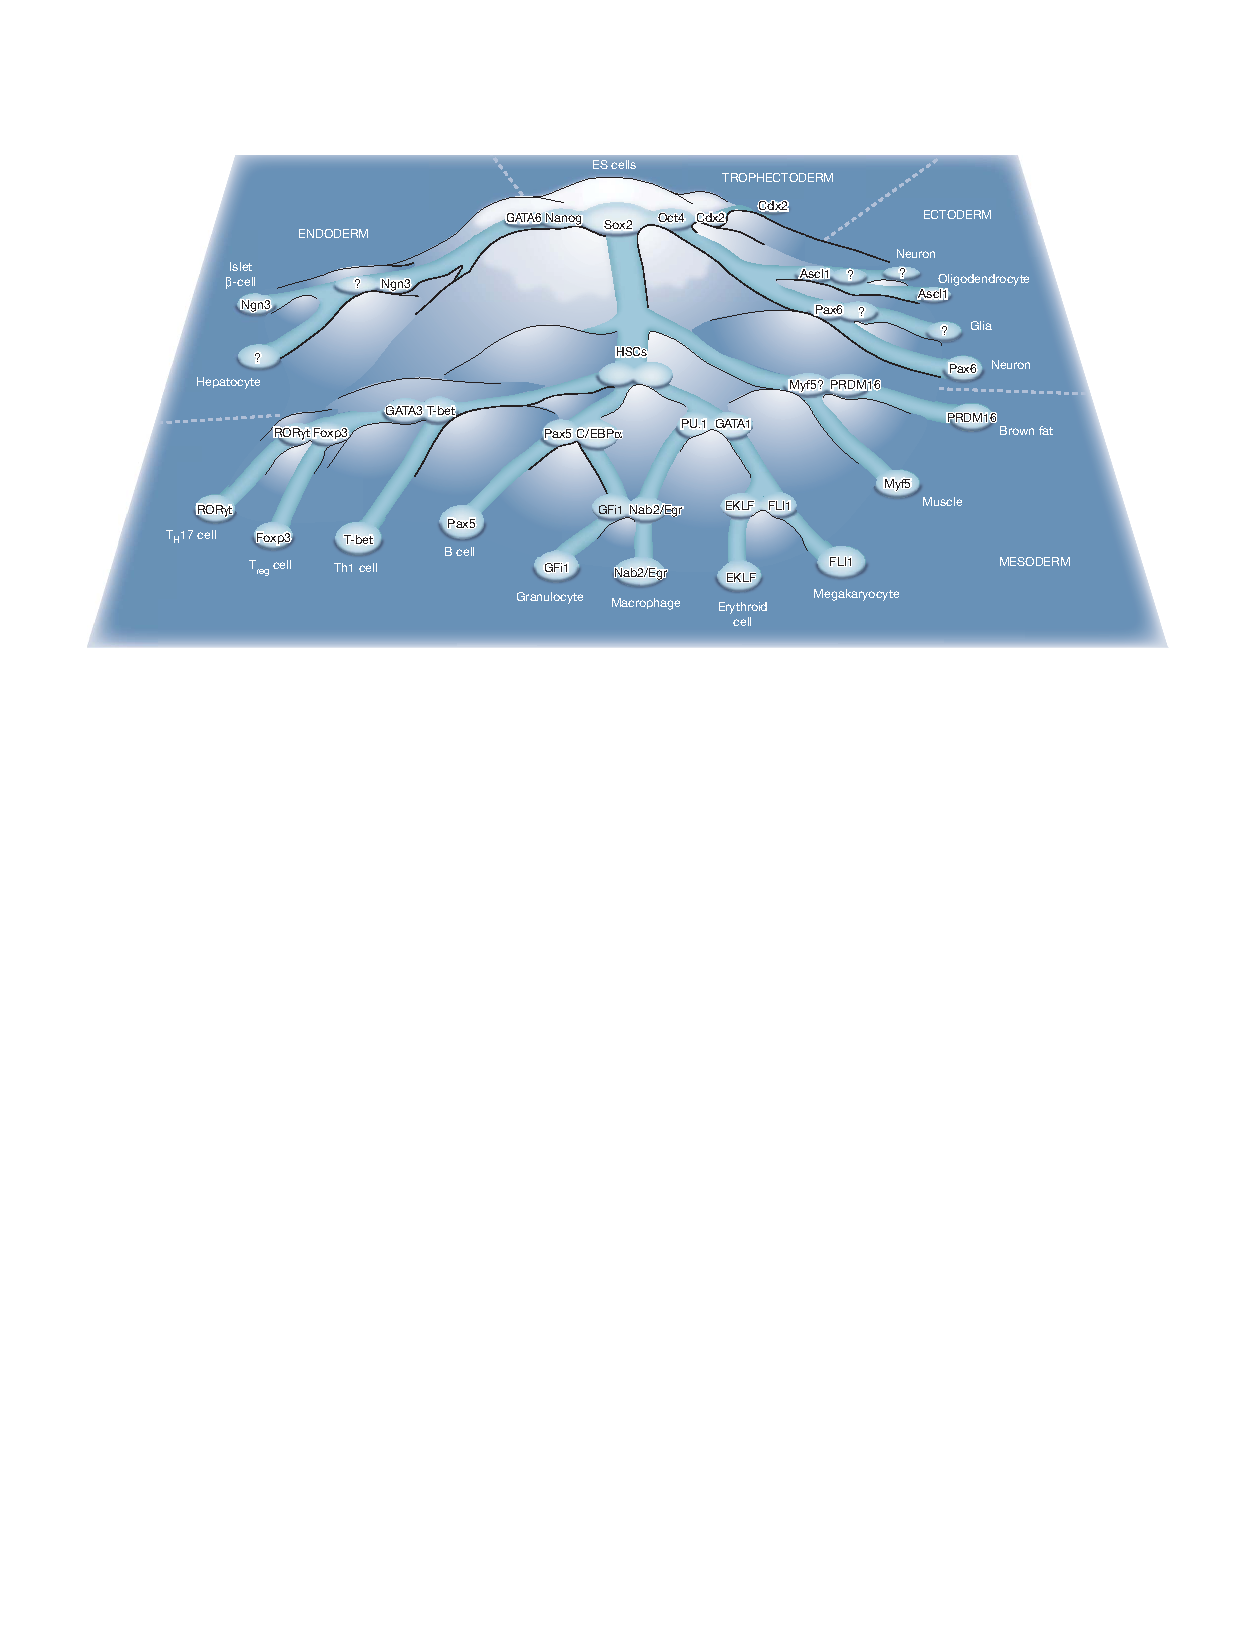
\includegraphics[width=\textwidth]{figures/graf-differentiation-landscape.pdf}
%\captionbf{Les antagonismes entre \tfs sculptent le paysage des destins
%cellulaires}{
%   Figure tir�e de \cite{Graf2009p2592}. Vision g�om�trique de la
%   diff�renciation cellulaire inspir�e de Waddington (voir
%   fig.\ref{fig:furusawa-epigenetic-landscape}).
%} 
%\efig
%

%\newpage
%\FloatBarrier
%\clearpage
%\newpage
\section{Pr�diction et validation des CRMs}
\label{sec:prediction_crms}

\bfig
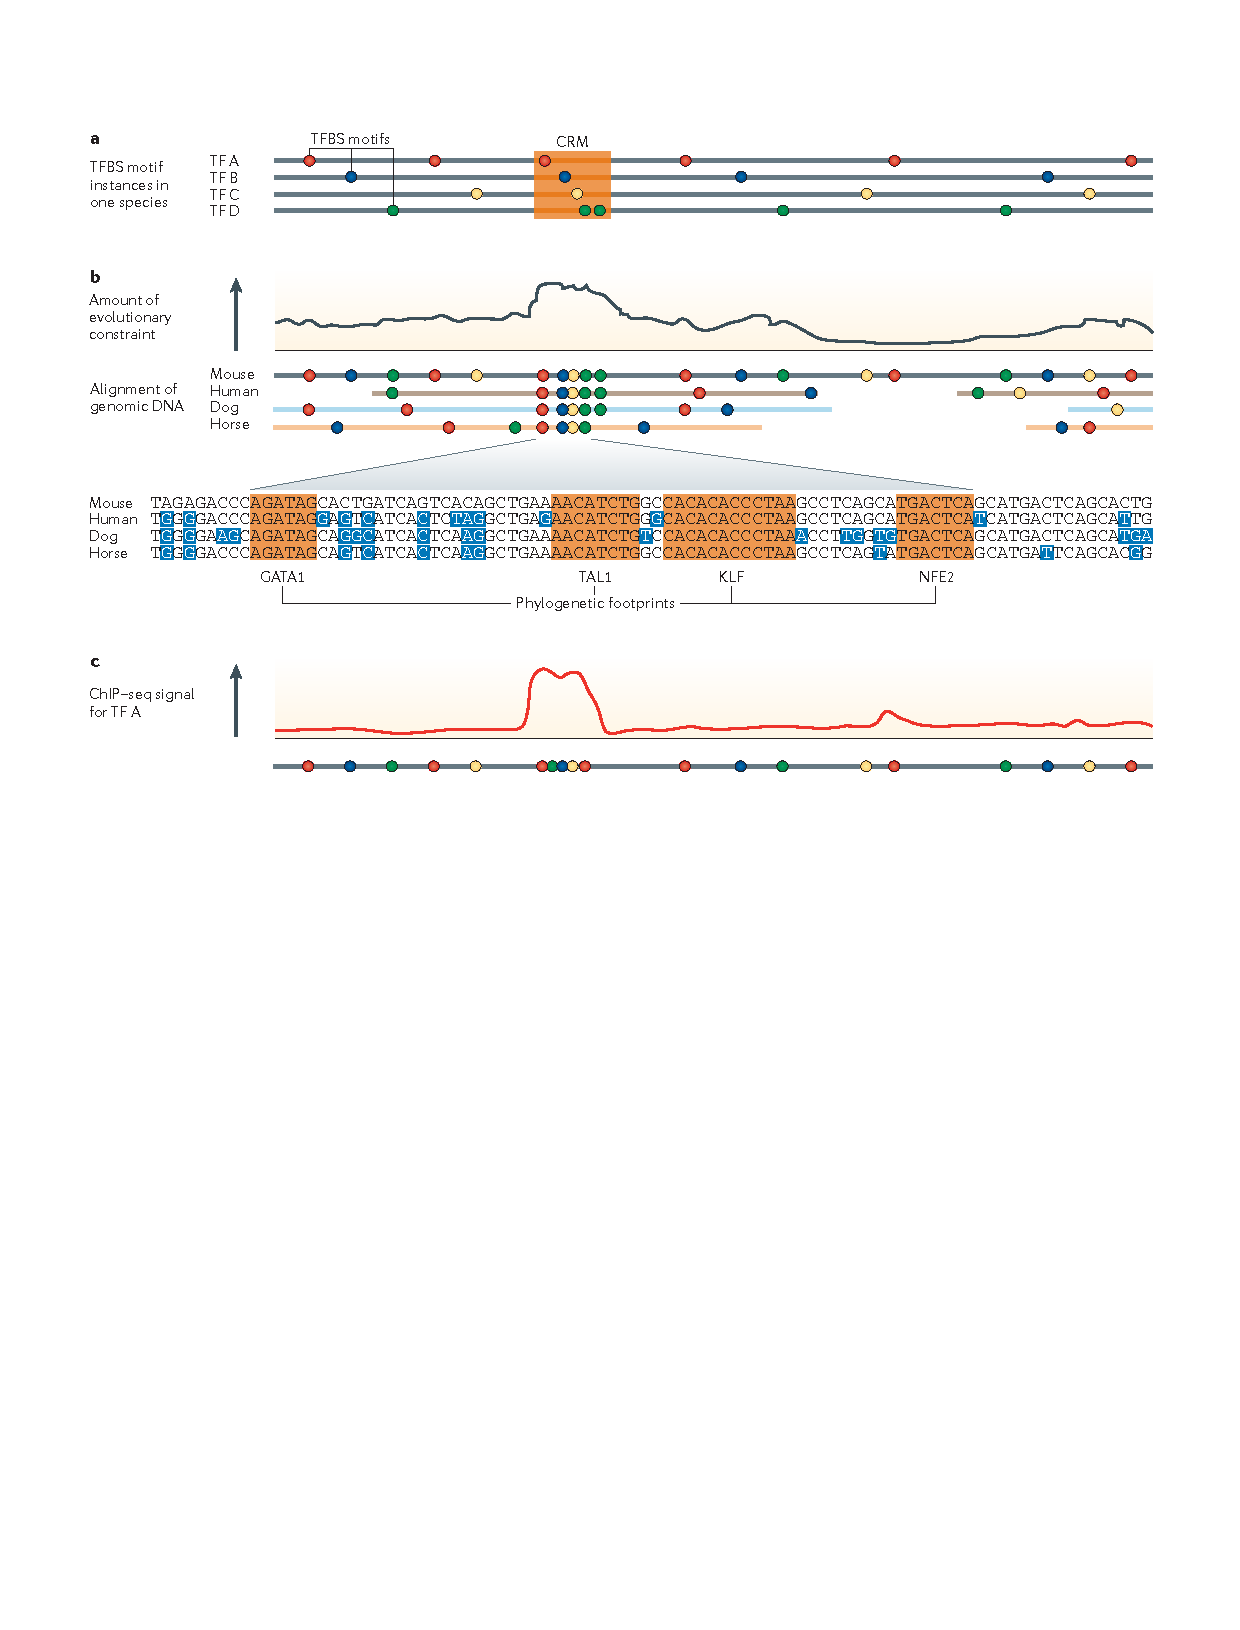
\includegraphics[width=\textwidth]{figures/hardison-CRM-prediction.pdf}
\captionbf{Diff�rentes approches pour la pr�diction des CRMs}{

    Figure tir�e de \cite{Hartwell1999p560}, r�sumant les diff�rentes approches
    de pr�diction des CRMs. (a) Pr�diction de sites sites de fixations (TFBS)
    pour diff�rents facteurs de transcription. Le regroupement ou
    \textit{clustering} de TFBS d�finit un CRM putatif. (b) Le CRM, poss�dant des
    contraintes fonctionnelles, est conserv� chez plusieurs esp�ces proches. La
    s�quence d'ADN correspondant au CRM (un enhancer connu de la
    $\beta$-globine) est montr�e chez les diff�rentes esp�ces. Les nucl�otides
    qui diff�rent par rapport � la s�quence de r�f�rence (la souris) sont
    indiqu�s en bleu, et les sites de fixation de TFs connus ou pr�dits sont
    indiqu�s en orange. Ceux-ci correspondent � des s�quences compl�tement
    conserv�es : on parle d'empreinte phylog�n�tique ou \textit{phylogenetic
    footprint}. (c) Une exp�rience de \chipseq sp�cifique au TF A produit un
    pic au niveau du CRM. Il est � noter que des pics peuvent exister m�me si
    aucun site de fixation n'est pr�dit, d� par exemple � une interaction
    prot�ine-prot�ine entre le TF A et un autre TF fix� � l'ADN.

} 
\label{fig:hardison-CRM-prediction}
\efig

\subsection{M�thodes utilisant la concentration en sites de fixation}
\label{sub:m_thodes_utilisant_la_concentration_en_sites_de_fixation}

Nous l'avons vu, une propri�t� des CRMs est leur grande concentration en TFBS.
Ceci a motiv� des approches de pr�diction de promoteurs et d'enhancers bas�es
sur leur contenu ou \textit{clustering} en motif
(fig.~\ref{fig:hardison-CRM-prediction}a). L'avantage de telles approches est
qu'elles peuvent �tre r�alis�es avec seulement la s�quence d'ADN g�nomique et
des mod�les de TFs ou motifs (par exemple des PWMs, voir fig.
\ref{fig:wasserman-PWM}) repr�sentant les \tfs impliqu�s dans le processus
�tudi�. Cependant, les clusters de motifs sont tr�s r�pandus dans les grands
g�nomes, et sans l'ajout d'informations suppl�mentaires comme les marques
�pig�n�tiques ou l'expression des g�nes voisins, ces approches produisent un
grand nombre de faux positifs (�l�ments pr�dits comme positifs mais �tant en
r�alit� n�gatifs). Par ailleurs, les TFs impliqu�s ne sont pas toujours connus,
et il faut alors apprendre des motifs putatifs � partir de s�quences
fonctionnelles.

\subsubsection{Approches utilisant des motifs connus}
\label{ssub:approches_utilisant_des_motifs_connus}

L'une des premi�res investigations bas�e sur le regroupement de TFBS utilisait
$5$ motifs connus de la d�termination musculaire pour pr�dire par r�gression
lin�aire les CRMs actifs dans le muscle~\cite{Wasserman1998p3779}. Le taux de
validation �tait relativement bas, autour de $20\%$. De m�me, chez \dmel,
plusieurs �tudes ont utilis� le clustering de motifs pour pr�dire des CRMs de
diff�rents processus d�veloppementaux (par ex \citet{Berman2002oq}). Ces �tudes
ont trouv� de nouveaux enhancers valid�s exp�rimentalement (bonne
sensibilit�) mais avaient des taux de pr�diction relativement bas, entre
$15$ et $30\%$.  L'algorithme \textit{Ahab}~\cite{Rajewsky2002kl}, utilisant un
mod�le thermodynamique de fixation des TFs sur les CRMs, a quant � lui r�ussi
� pr�dire un nombre bien plus important de r�gions fonctionnelles : $\sim80\%$
des modules pr�dits � proximit� de $29$ g�nes de segmentation chez la
drosophile ont effectivement r�capitul� le motif d'expression du g�ne
associ�~\cite{Schroeder2004tg}. Ce succ�s semble notamment �tre d� au fait que
ce mod�le thermodynamique, bas� sur une prise en compte exhaustive de toutes
les segmentations possibles des CRMs en motifs et en ADN \og background \fg,
permet de donner plus de poids au cas o� plusieurs sites de faibles affinit�
pour un TF se trouvent au sein d'un m�me module, alors que les autres m�thodes
utilisent g�n�ralement un seuil de probabilit� relativement �lev� (afin
d'�viter les faux positifs) � partir duquel une s�quence est consid�r�e comme
fix�e par un TF. Par ailleurs, cette �tude s'est restreinte � un ensemble de
g�nes connus pour lesquels les r�gions � proximit� riches en TFBS ont \apriori
plus de chances d'�tre fonctionnelles. De mani�re g�n�rale, plus le domaine de
recherche est �tendu (par exemple, le g�nome entier), plus le nombre de faux
positifs augmente.


% subsubsection approches_utilisant_des_motifs_connus (end)

\subsubsection{Approches \denovo o� les motifs ne sont pas connus}
\label{ssub:approches_denovo_o_les_motifs_ne_sont_pas_connus}

Lorsque les motifs (PWMs) ne sont pas connus � l'avance, il faut les g�n�rer
\denovo � partir de leur surrepr�sentation dans des CRMs connus. Par exemple,
l'algorithme CisModule permet de g�n�rer des motifs et des modules
simultan�ment en utilisant un mod�le de m�lange hi�rarchique~\cite{Zhou2004hc}.
Lorsqu'il est appliqu� aux CRMs musculaires introduits pr�c�demment, il permet
de retrouver certains motifs connus et permet de retrouver $\sim70-80\%$ des
s�quences connues lorsqu'elle sont m�lang�es avec un nombre similaire de
s�quences al�atoires. Par ailleurs, l'apprentissage de mod�les permettant de
discriminer diff�rentes classes de CRMs entre elles plut�t qu'une classe de
CRMs par rapport � des s�quences al�atoires ou interg�niques peut s'av�rer plus
fructueux. Ainsi, \cite{Smith2006ij} ont utilis� des motifs connus ainsi que
des motifs appris \textit{de novo} avec le programme DME~\cite{Smith2005bs}
pour leur capacit� � discriminer des s�quences appartenant � diff�rents jeux de
donn�es de r�gions promotrices pour b�tir un mod�le de r�gression logistique
permettant de pr�dire l'activit� tissu-sp�cifique dans $45$ des $56$ tissus
humains et murins consid�r�s. Il existe aussi plusieurs m�thodes qui
n'utilisent pas de motifs du type PWM, mais de purs mod�les probabilistes tels
que des cha�nes de Markov d'ordre $5$ ou des regroupements de \og mots \fg de
$k$ nucl�otides ou $k$-mers selon des crit�res de distance de Hamming et
surrepr�sent�s dans les s�quences d'int�r�t, par exemple~\cite{Cao2010p1805}.
Ces m�thodes sont pass�es en revue dans \cite{Kantorovitz2009p2937}, et elles
peuvent atteindre des sensibilit�s de $\sim60\%$ pour la pr�diction de CRMs
mammif�res. L'int�r�t est que ces �tudes ne pr�sument pas d'un mod�le de
fixation des TFs � l'ADN. C'est aussi un d�savantage, puisqu'elles sont moins
informatives quant au r�seau g�n�tique sous-jacent et aux m�canismes de
r�gulation impliqu�s.

% subsubsection approches_denovo_o_les_motifs_ne_sont_pas_connus (end)


% subsection m_thodes_utilisant_la_concentration_en_sites_de_fixation (end)

\subsection{M�thodes utilisant la phylog�nie}
\label{sub:m_thodes_utilisant_la_phylog_nie}

Les approches utilisant la comparaison des g�nomes de diff�rentes esp�ces pour
pr�dire des CRMs sont bas�es sur l'id�e que les s�quences de r�gulation sont
plus fortement conserv�es que l'ADN non fonctionnel les entourant. Nous l'avons
vu en \ref{sub:evolution-des-enhancer}, une proportion importante de CRMs ne
satisfont pas � cette r�gle. Cette approche ne permet donc d'�tudier que le
sous-ensemble de CRMs qui a subi une forte pression de s�lection depuis le
dernier anc�tre commun aux esp�ces consid�r�es et ne donne pas acc�s aux CRMs
apparus r�cemment au sein d'une esp�ce.

\subsubsection{Pr�dictions � partir de la contrainte �volutive seule}
\label{ssub:pr_dictions_partir_de_la_contrainte_volutive_seule}

L'alignement de s�quences non-codantes orthologues fait appara�tre des parties
tr�s conserv�es, avec peu de variations dans les s�quences sous-jacentes,
entour�es de s�quences accumulant les variations
(fig.~\ref{fig:hardison-CRM-prediction}b). De telles s�quences conserv�es sont
alors interpr�t�es comme ayant �t� sous s�lection, les substitutions d�l�t�res
ayant �t� rejet�es au cours de l'�volution~\cite{Dermitzakis2005kl}. Par
analogie avec les empreintes � la DNAse I, on parle d'empreinte phylog�n�tique
pour caract�riser ces courtes s�quences tr�s conserv�es ($\sim10$bp), traces de
la fixation putative d'un facteur de transcription.  Ces empreintes s'av�rent
�tre un indicateur fiable de fonctionnalit�~\cite{Kheradpour2007mi} et, parce
qu'elles ne reposent pas sur des mod�les \apriori de fixation, elles permettent
de plus de trouver des motifs de r�gulation non connus~\cite{Xie2005pi}. Au
niveau de s�quences plus longues ($\sim100$bp), la contrainte �volutive permet
de d�tecter des CRMs entiers. Ainsi, comme nous l'avons vu en
\ref{sub:evolution-des-enhancer}, l'utilisation de la conservation extr�me
permet d'atteindre $50\%$ de taux validation~\cite{Pennacchio2006vn}.
N�anmoins, lorsque ces contraintes de conservation extr�me (par exemple
homme-\textit{Fugu}) sont rel�ch�es, le taux de validation tombe drastiquement,
atteignant $\sim5\%$~\cite{Attanasio2008ff}, montrant la n�cessit� d'allier le
crit�re de conservation � d'autres donn�es (expression, ChIP\ldots) pour
am�liorer la pr�diction des CRMs.


% subsubsection pr_dictions_partir_de_la_contrainte_volutive_seule (end)

\subsubsection{Pr�dictions utilisant la phylog�nie et des motifs connus}
\label{ssub:pr_dictions_utilisant_la_phylog_nie_et_des_motifs_connus}

Une approche pour am�liorer les pr�dictions est de combiner les approches
pr�c�dentes en utilisant � la fois le \textit{clustering} en TFBS et la
contrainte �volutive. � l'�chelle du g�nome entier, cette approche permet de
filtrer les r�sultats pour am�liorer le signal de d�tection chez la
Drosophile~\cite{Sinha2004lh}.  Du c�t� des mammif�res, en utilisant les motifs
de la base de donn�es TRANSFAC et la conservation entre l'homme et la souris,
\citet{Blanchette2006fu} ont cr�� une base de donn�es de modules, PReMods, qui
retrouve $\sim17\%$ de CRMs connus et recoupe $40\%$ des fragments occup�s par
le co-activateur et marqueur de l'activit� enhancer p$300$. D'autres
m�thodes se sont concentr�es sur des types cellulaires bien d�finis. Par
exemple, la recherche de sites conserv�s pour des motifs de TF des cellules
sanguines connus ~\cite{Donaldson2005ye} a permis de d�finir des CRMs dont $2$
ont �t� test�s et valid�s. 

Certains efforts ont par ailleurs �t� men�s pour sortir du cadre d'une
conservation de s�quence stricte en mod�lisant l'�volution d'un CRM fix� par un certain
nombre de motifs connus. Par exemple, le mod�le MorphMS~\cite{Sinha2007tw}
cherche au sein d'un alignement de deux s�quences orthologues des r�gions
pr�dites par un mod�le d'�volution d�riv� d'un ensemble de motifs choisis par
l'utilisateur. Une extension de cette approche incorpore le gain et la perte de
sites de fixation, mais n'a cependant pas encore �t� appliqu�e � l'�chelle du
g�nome~\cite{Majoros2010il}.

% subsubsection pr_dictions_utilisant_la_phylog_nie_et_des_motifs_connus (end)

\subsubsection{Approches utilisant la phylog�nie pour g�n�rer des motifs \denovo}
\label{ssub:approches_utilisant_la_phylog_nie_pour_g_n_rer_des_motifs_denovo}

De m�me que pr�c�demment, tous les motifs ne sont pas connus et il peut �tre
utile d'avoir recours � de l'apprentissage direct � partir de s�quences
fonctionnelles connues pour aider � la pr�diction. Par exemple, l'algorithme
ESPER cherche des patterns (TFBS, \%GC, etc) surrepr�sent�s dans des
alignements multi-esp�ces de CRMs connus par rapport � des alignements d'ADN
\apriori non fonctionnel~\cite{Taylor2006zt}. Cette m�thode n'est pas
restreinte � l'analyse de s�quences conserv�es puisqu'elle peut potentiellement
capturer des signatures de changements syst�matiques. La pr�diction de r�gions
de haut potentiel de r�gulation recouvre presque enti�rement les pr�dictions de
PReMods, et le test par transfection de ces r�gions � proximit� de g�nes
exprim�s dans les cellules �rythro�des et poss�dant un site pour un TF
sp�cifique de l'�rythro�de m�ne � un taux de validation de $50\%$. Une autre
m�thode consiste � chercher des mots surrepr�sent�s dans un ensemble
d'apprentissage de CRMs connus puis � restreindre les pr�dictions aux r�gions
conserv�es~\cite{Kantorovitz2009p2937}. Les pr�dictions r�alis�es ont toutes
�t� valid�es chez la Drosophile ($5/5$) comme chez la souris ($2/2$).

% subsubsection approches_utilisant_la_phylog_nie_pour_g_n_rer_des_motifs_denovo (end)


\subsection{M�thodes utilisant les marques �pig�n�tiques et de \chipseq pour des TFs}
\label{sub:m_thodes_utilisant_les_marques_pig_n_tiques}

\subsubsection{Pr�diction des promoteurs}
\label{ssub:pr_diction_des_promoteurs}

La m�thode la plus fiable de pr�diction d'un promoteur utilise le fait qu'il
est toujours localis� au niveau d'un TSS, dont la position peut facilement �tre
obtenue en alignant les s�quences de l'ARN du g�ne correspondant sur le
g�nome~\cite{Trinklein2003jl}. Le taux de validation avec cette seule
contrainte est tr�s �lev� : $91\%$ ont une activit� dans au moins un type
cellulaire. Par ailleurs, la marque �pig�n�tique H3K4me$3$ est aussi un
indicateur des promoteurs actifs dans le type cellulaire �tudi�
\cite{Heintzman2007gb} (fig.~\ref{fig:hardison-enhancer-states}).

% subsubsection pr_diction_des_promoteurs (end)

\subsubsection{Pr�diction des enhancers}
\label{ssub:pr_diction_des_enhancers}

La pr�diction des enhancers � partir des marques �pig�n�tiques, comme
l'ac�tylation des histones~\cite{Roh2005mb}, la m�thylation H3K4me$1$
\cite{Heintzman2009ys}, ou encore la pr�sence du co-activateur
p$300$~\cite{Visel2009p3750}, est tr�s efficace, avec une expression
tissue-sp�cifique dans $\sim80\%$ des cas~\cite{Hardison2012p3778}. Par exemple,
ces diff�rentes marques, pr�sentes dans diff�rents tissus, peuvent �tre
utilis�es comme autant d'entr�es d'un mod�le de Markov cach� pour produire des
pr�dictions fiables de CRMs tissu-sp�cifiques chez l'homme~\cite{Ernst2011cq}. 

En fait, les pr�dictions d'activit� enhancer � partir de ces marques
�pig�n�tiques est plus fiable qu'en utilisant la fixation de \fts
tissu-sp�cifiques. Par exemple, sur $63$ s�quences ADN fix�es \invivo par le
facteur sp�cifique des cellules sanguines GATA$1$ chez la souris, seulement la
moiti� conduisent � une activit� apr�s transfection dans des cultures
cellulaires~\cite{Cheng2008fk}. Ces enhancers fonctionnels sont par ailleurs
plus particuli�rement associ�s � un site de fixation \textit{conserv�} pour
GATA$1$, montrant � nouveau la n�cessit� de combiner les approches pour
am�liorer la d�tection. Un taux de validation similaire a �t� observ� pour le
facteur de diff�renciation myog�nique MyoD, avec $40\%$ de r�gions fix�es ayant
une activit� apr�s transfection en cellules.

L'utilisation de donn�es de fixation pour plusieurs TFs � la fois semble
cependant am�liorer le pouvoir de pr�diction. Ainsi, \citet{Tijssen2011kx} ont
�tudi� la co-fixation de GATA$1$ avec $4$ autres TFs h�matopo��tiques dans des
m�gacaryocytes. En s'int�ressant aux g�nes � proximit� de ces r�gions, ils en
ont d�couvert plusieurs qui n'�taient pas pr�c�demment connus comme �tant
important dans l'h�matopo��se. Leur fonction a �t� test�e par knock-down, avec
dans $8$ cas sur les $9$ test�s une r�duction de la production de globules
rouges. 


% subsubsection pr_diction_des_enhancers (end)

% subsection m_thodes_utilisant_les_marques_pig_n_tiques (end)

% subsection m_thodes_utilisant_la_phylog_nie (end)


\bfig
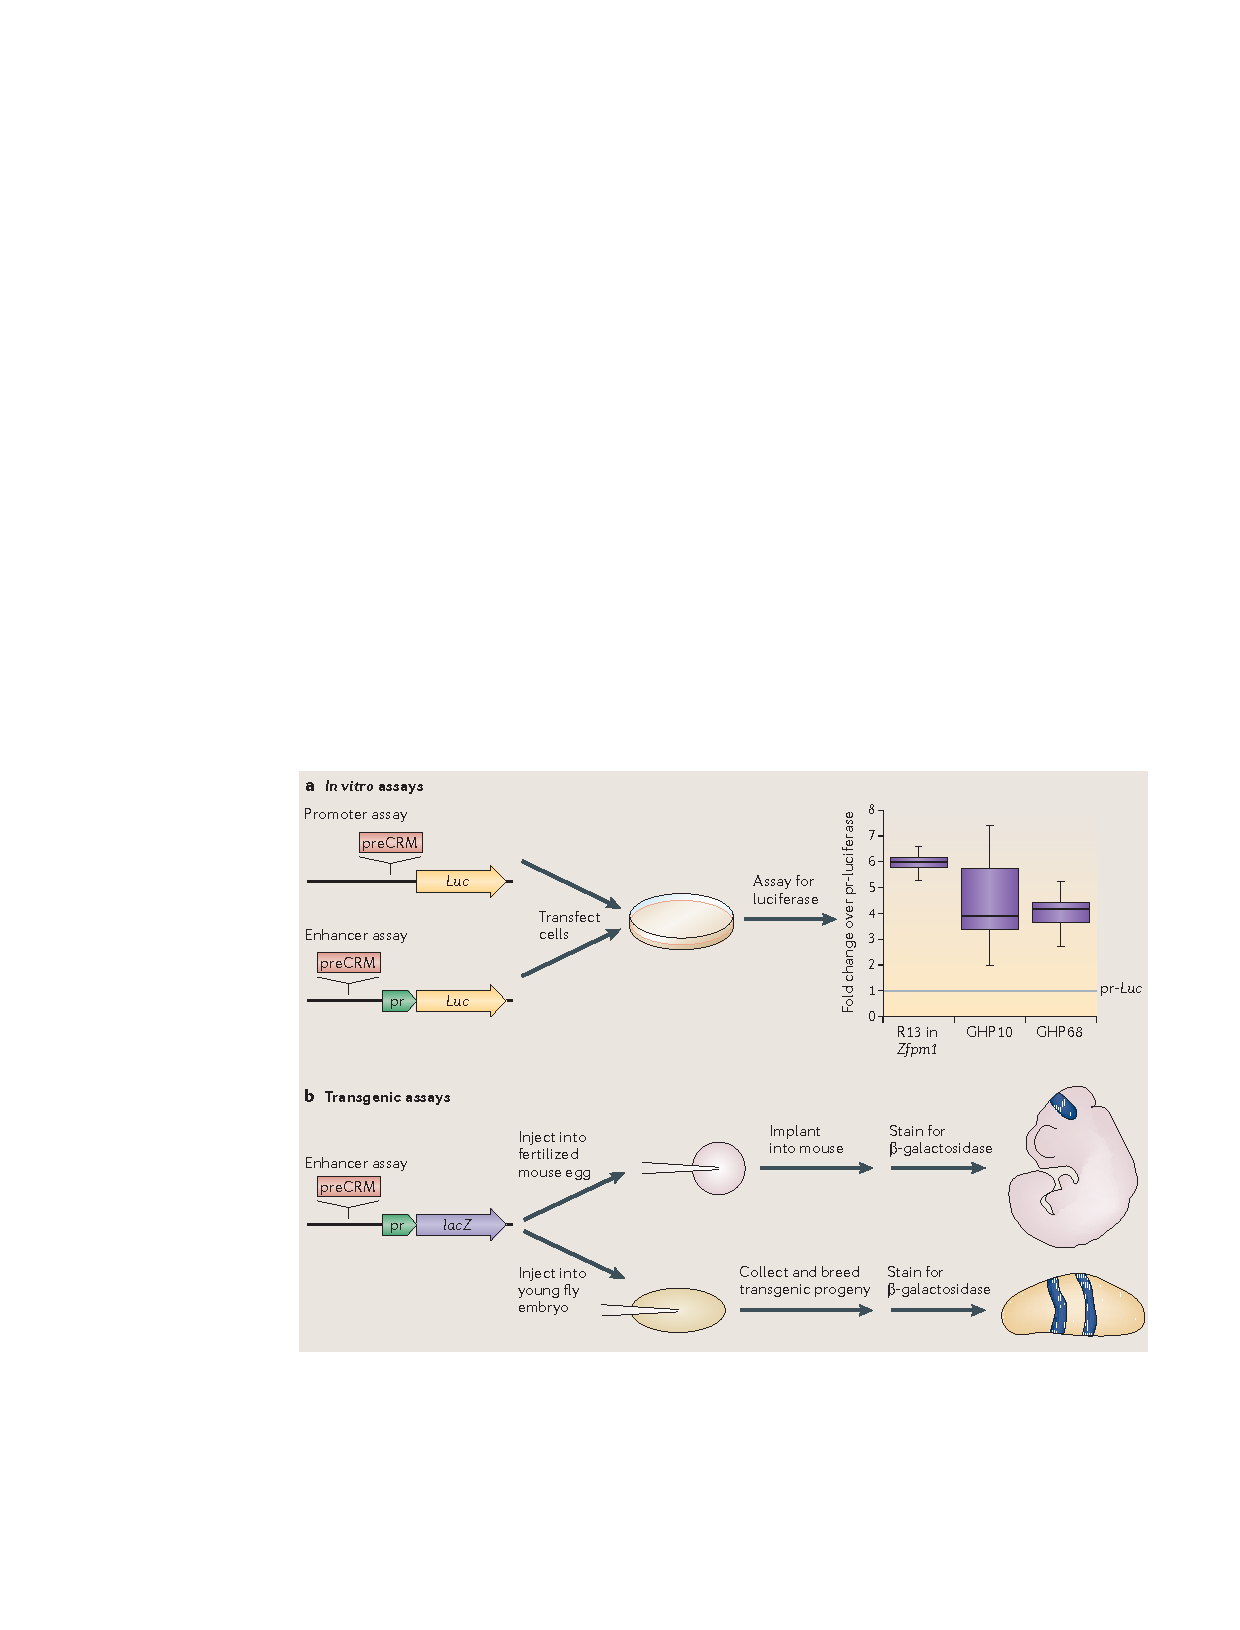
\includegraphics[width=\textwidth]{figures/hardison-CRM-test.pdf}
\captionbf{M�thodes de validation des CRMs par transfection et transgen�se}{
    
    Figure tir�e de \cite{Hartwell1999p560} pr�sentant les m�thodes \invitro et
    \invivo de validation des CRMs. La r�gion dont on souhaite tester
    l'activit� est ins�r�e dans un plasmide codant pour un g�ne rapporteur qui
    est transf�r� dans une culture cellulaire (transfection, panel a) ou dans
    un organisme entier (transgen�se, panel b). Dans le cas du test d'un
    promoteur, le CRM est plac� directement en amont du g�ne rapporteur (on
    utilise g�n�ralement la lucif�rase \textit{Luc}), alors que dans le cas
    d'un enhancer, le CRM est plac� en amont d'un promoteur minimal de faible
    activit�. L'activit� de la lucif�rase donne une information quantitative
    sur l'activit� de la r�gion test�e (bo�tes � moustache, panel a). Dans le
    cas d'une transgen�se, le g�ne rapporteur g�n�ralement utilis� est
    \textit{lacZ} qui encode la $\beta$-galactosidase. La r�v�lation par
    coloration permet de visualiser en bleu les tissus au sein lesquels
    l'enhancer est actif.

} 
\label{fig:hardison-CRM-test}
\efig

\subsection{Validation exp�rimentale}
\label{sub:validation_experimentale}

%Il existe plusieurs m�thodes pour s'assurer de la fonctionnalit� d'un CRM pr�dit. 

%Tout d'abord, une m�thode indirecte donnant du cr�dit � la pr�diction d'un CRM
%est d'examiner le motif d'expression du g�ne dont le TSS est le plus proche. Si
%cette expression reproduit les caract�ristiques utilis�es pour pr�dire le CRM
%(par exemple, s'exprimer dans le muscle pour une pr�diction de CRMs utilisant
%l'abondance de sites de liaison de TFs musculaires), alors cela soutient l'id�e
%(mais ne la d�montre pas) que la pr�sence du CRM en est la cause.

Une m�thode %plus 
directe permettant de d�montrer qu'un fragment d'ADN r�gule
l'expression g�n�tique consiste en une exp�rience de gain de fonction dans
laquelle un plasmide contenant le CRM pr�dit � proximit� d'un g�ne rapporteur
est introduit par transfection \invitro en cellule, permettant un suivi
quantitatif de l'activit�, ou par transgen�se \invivo dans un organisme, auquel
cas le suivi est plus qualitatif mais permet d'�tablir la sp�cificit�
spatio-temporelle (tissu et stade de d�veloppement) de l'�l�ment de r�gulation
(fig.~\ref{fig:hardison-CRM-test}). Ce type d'exp�rience montre que le CRM
pr�dit est \textit{suffisant} pour reproduire le motif g�n�tique observ�. De
mani�re optimale, il faudrait aussi montrer par d�l�tion cibl�e de l'�l�ment de
r�gulation au sein du g�nome que ce dernier est \textit{n�cessaire}
� l'expression du g�ne endog�ne.

\FloatBarrier

\subsection{Implication des CRMs dans les maladies humaines}
\label{sub:implication_des_crms_dans_les_maladies_humaines}

\bfig
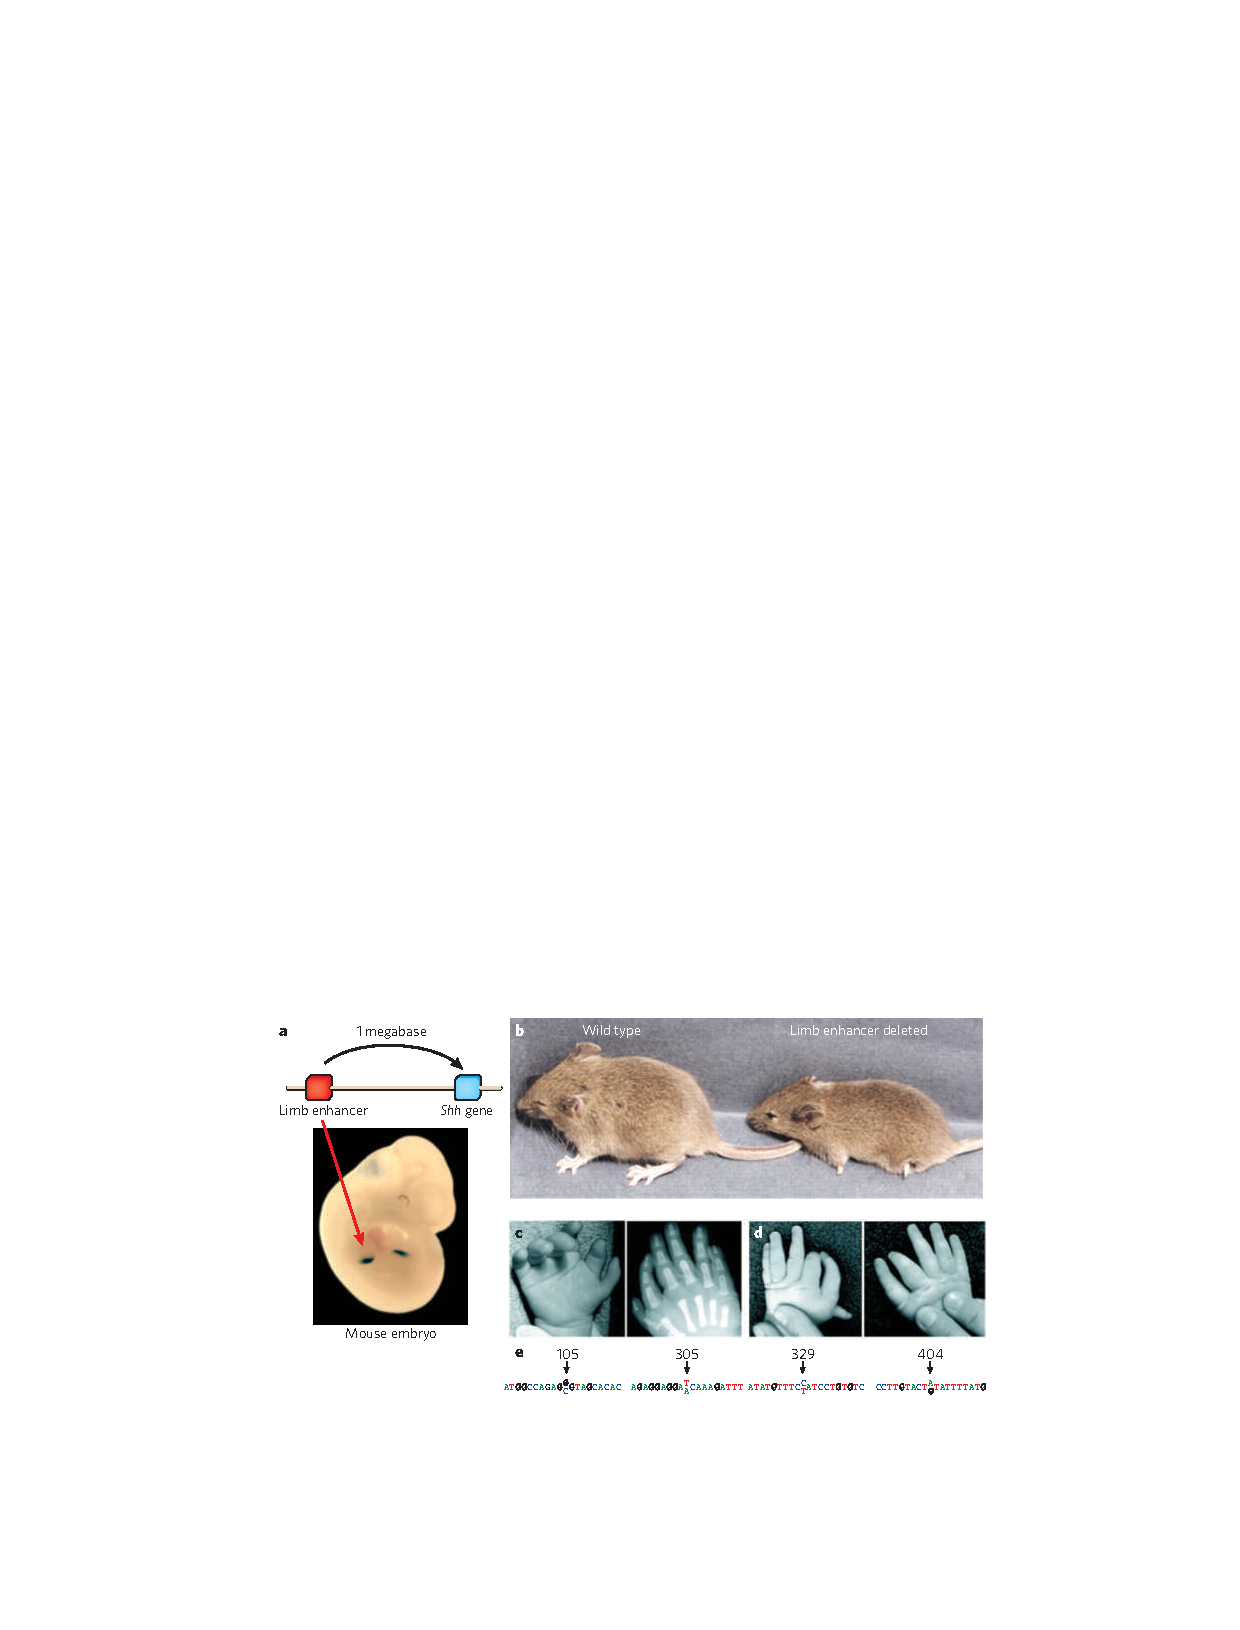
\includegraphics[width=1.0\textwidth]{figures/visel-shh-CRM-medical.pdf}
\captionbf{Impact physiologique de la d�l�tion et de la mutation d'un enhancer}{

Figure tir�e de~\cite{Visel2009kx}. (a) L'enhancer \og membre \fg de
\textit{Sonic hedgehog} (\textit{Shh}) est situ� � $\sim1$ Mb de son g�ne
cible, au sein d'un intron d'un g�ne voisin. Par transgen�se il conduit
l'expression d'un rapporteur dans la partie post�rieure du bourgeon de membre
chez l'embryon de souris~\cite{Lettice2003uq}. (b) Les souris poss�dant une
d�l�tion cibl�e de cet enhancer poss�dent des membres tronqu�s, montrant son
importance fonctionnelle au cours du d�veloppement~\cite{Sagai2005cr}. (c-e)
Diff�rentes mutations ponctuelles dans la s�quence enhancer orthologue chez
l'homme r�sultent en une polydactilie pr� axiale (pr�sence de doigts ou orteils
suppl�mentaires), montrant l'impact potentiel de variations dans des r�gions
non-codantes~\cite{Lettice2003uq}.

}
\label{fig:visel-shh-CRM-medical}
\efig


Au cours des derni�res d�cennies, de nombreuses mutations dans les r�gions
codantes des g�nes, impliquant des d�fauts structurels des prot�ines
associ�es, ont pu �tre associ�es � des maladies g�n�tiques. � l'inverse, le
r�le des mutations affectant des r�gions non codantes n'a �t� que peu explor�,
essentiellement du fait de la difficult� d'annoter ces r�gions correctement
afin de d�finir celles qui pourraient avoir une fonction d'int�r�t. Plusieurs
�tudes ont cependant pu montrer que des variations affectant des enhancers
distaux pouvaient conduire � des pathologies~\cite{Visel2009kx}.


L'une de ces �tudes concerne l'enhancer sp�cifique du membre de \textit{Shh}
(fig.~\ref{fig:visel-shh-CRM-medical}). Cet enhancer, initialement d�crit chez
la souris, se situe � environ $1$ Mb de distance de \textit{Shh}, au sein de
l'intron d'un g�ne voisin. Le s�quen�age de cet enhancer chez plusieurs
individus humains a permis d'associer une douzaine de variations
mono-nucl�otidiques � la polydactilis pr� axiale, \cad la pr�sence de doigts ou
d'orteils suppl�mentaires~\cite{Lettice2003uq}.  Des �tudes suppl�mentaires
chez la souris ont montr� que les variations de s�quences observ�es dans cet
enhancer conduisent � une expression ectopique dans la partie ant�rieure du
membre au cours du d�veloppement, ce qui est consistent avec la pr�sence de
doigts suppl�mentaires~\cite{Masuya2007nx}. Par ailleurs, la d�l�tion de
l'enhancer orthologue de la souris entra�ne la troncation des
membres~\cite{Sagai2005cr}. 

Ainsi, ces r�sultats montrent l'importance de l'identification des enhancers
pour permettre � des �tudes de g�n�tique humaine d'explorer le r�le
potentiellement pathologique de mutations dans des r�gions non codantes
fonctionnelles.

% subsection implication_des_crms_dans_les_maladies_humaines (end)
%\FloatBarrier
%\newpage
\section{Bases de donn�es}

La biologie moderne est caract�ris�e par l'accumulation de donn�es biologiques
qu'il s'agit d'int�grer puis d'interpr�ter : on parle de biologie integrative.
En particulier, depuis le s�quen�age du g�nome humain il y a maintenant plus de
dix ans~\cite{Lander2001p1633}, le nombre de g�nome s�quenc�s n'a cess�
d'augmenter, tandis que dans le m�me temps le prix du s�quen�age diminuait
drastiquement (fig.~\ref{fig:sboner-cost-sequencing.jpg}). Afin de permettre la
gestion et l'utilisation de ces donn�es, de nombreux outils et bases de donn�es
ont �t� mis � disposition~\cite{Wasserman2004p624}. Nous �voquons ici ceux qui
nous paraissent essentiels du point de vue de la r�gulation en \textit{cis}.

\bfig
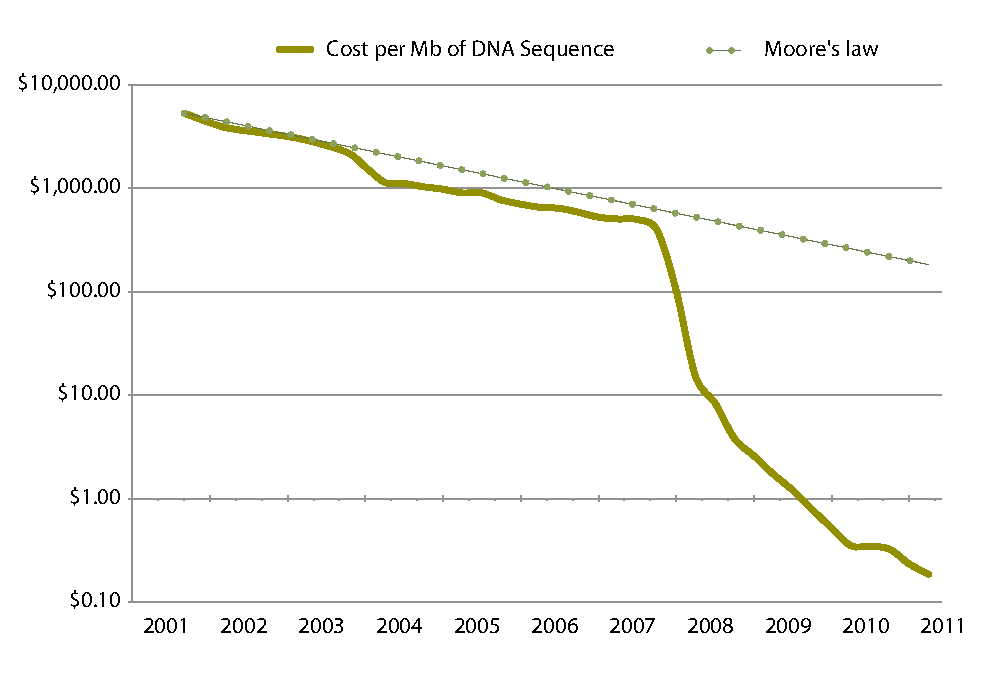
\includegraphics[width=0.8\textwidth]{figures/sboner-cost-sequencing.pdf}
\captionbf{�volution du co�t de s�quen�age}{

Figure adapt�e de~\cite{Sboner2011fk}, montrant l'�volution du co�t du
s�quen�age d'$1$ Mb d'ADN au cours de la derni�re d�cennie, compar� � une
�volution de type \og Loi de Moore \fg o� le prix serait diminu� de moiti� tous
les $18$ mois.

}
\label{fig:sboner-cost-sequencing.jpg}
\efig


\subsection{Obtention de donn�es g�nomiques}
\label{sub:obtention_donnees_genomiques}

Tout d'abord, les diff�rents g�nomes s�quenc�s sont � disposition sur des bases
de donn�es publiques d'o� ils peuvent �tre t�l�charg�s puis analys�s en aval.
Parmi les plus g�n�ralistes se trouvent la base de donn�e de UCSC
(UCSC Genome Browser, \url{http://genome.ucsc.edu}) et celle de l'EMBL (Ensembl,
\url{http://www.ensembl.org}) \footnote{Les donn�es sont accessibles sur les
    pages de t�l�chargement, respectivement
    \url{http://hgdownload.cse.ucsc.edu/downloads.html} pour UCSC et
    \url{http://www.ensembl.org/info/data/ftp/index.html} pour Ensembl 
}. 

Sont � disposition les g�nomes des diff�rentes esp�ces s�quenc�es pour les
diff�rents assemblages r�alis�s, des alignements des g�nomes de diff�rentes
esp�ces deux par deux (\textit{pairwise alignments}) ou par groupes d'esp�ces
(\textit{multiple alignments}), ainsi qu'un certain nombre d'annotations
essentielles � l'analyse de ces g�nomes : coordonn�es des g�nes (TSSs, exons,
introns avec potentiellement diff�rents transcrits alternatifs), miRNA ou
lincRNA, ontologies associ�es, coordonn�es des s�quences r�p�titives (les
\textit{repeats}, en partie li�s aux �l�ments transposables abord�s en
\ref{sub:evolution-des-enhancer}, et qui sont abondants dans les g�nomes
vert�br�s), diff�rentes donn�es \chipseq, indices de conservation
\footnote{Pour le cas de l'assemblage mm$9$ de la souris, ces annotations sont
    accessibles � l'adresse suivante
    : \url{http://hgdownload.cse.ucsc.edu/goldenPath/mm9/database/} 
}\ldots 

Au final, ces diff�rentes donn�es constituent une base de travail fiable et
r�guli�rement mise � jour. Afin de faciliter leur obtention, il est possible
d'utiliser le navigateur de tables de UCSC \footnote{
    \url{http://genome.ucsc.edu/cgi-bin/hgTables} } ou la section BioMart
    d'Ensembl \footnote{ \url{http://www.ensembl.org/biomart/martview} } .

Situ� plus en amont, le projet Galaxy (\url{http://galaxyproject.org}) permet
� l'utilisateur de r�cup�rer des donn�es depuis les diff�rentes banques
existantes, puis de leur faire subir divers traitements et analyses par divers
outils de bioinformatique. Cet outil, qui peut �tre utilis� sur internet ou
bien localement, a l'avantage de permettre la sauvegarde de plans de travail ou
\textit{workflows}, successions de commandes utilis�es pour traiter une entr�e
donn�e par diff�rents outils st�r�otyp�s et obtenir directement le r�sultat
final, favorisant une approche conviviale orient�e utilisateur.

En guise d'exemple, nous montrons en annexe \ref{ann:statistiques} des
statistiques obtenues ais�ment � partir d'annotations g�n�tiques pr�sentes sur
UCSC et trait�es avec Galaxy. Ces statistiques sont les distribution de tailles
des r�gions interg�niques et introniques chez plusieurs esp�ces : la bact�rie
\ecoli, la levure \textit{Saccharomyces cerevisiae}, le ver \celegans, la
mouche \dmel, la souris, le poulet et l'homme
(fig.~\ref{fig:intergenic-intronic}).

\subsection{Obtention de donn�es sur les TFs}
\label{sub:obtention_donnees_TFs}

Nous l'avons vu, les donn�es de fixation des TFs (\chipseq, \chipchip) peuvent
�tre obtenues � partir du site UCSC Genome Browser. Ces donn�es sont aussi
g�n�ralement accessibles sur le site du NCBI (Gene Expression Omnibus,
\url{http://www.ncbi.nlm.nih.gov/geo/}) \textit{via} un num�ro d'accession
donn� lors de la publication des donn�es. 

De nombreux mod�les de TFs ont d�j� �t� b�tis pr�alablement � l'av�nement des
donn�es haut-d�bit de type \chipseq, par exemple avec des donn�es SELEX, et il
existe des bases de donn�es stockant les PWMs correspondantes : JAPSAR, base de
donn�e publique \footnote{\url{http://jaspar.cgb.ki.se}}, et TRANSFAC, qui
marche par
abonnement\footnote{\url{http://www.gene-regulation.com/pub/databases.html}}.
Il est � noter que ces PWMs ayant souvent �t� construites � partir d'un faible
nombre de sites de fixations et de donn�es \invitro, elles peuvent �tre
relativement inadapt�es � l'analyse de donn�es \invivo.

\bfig
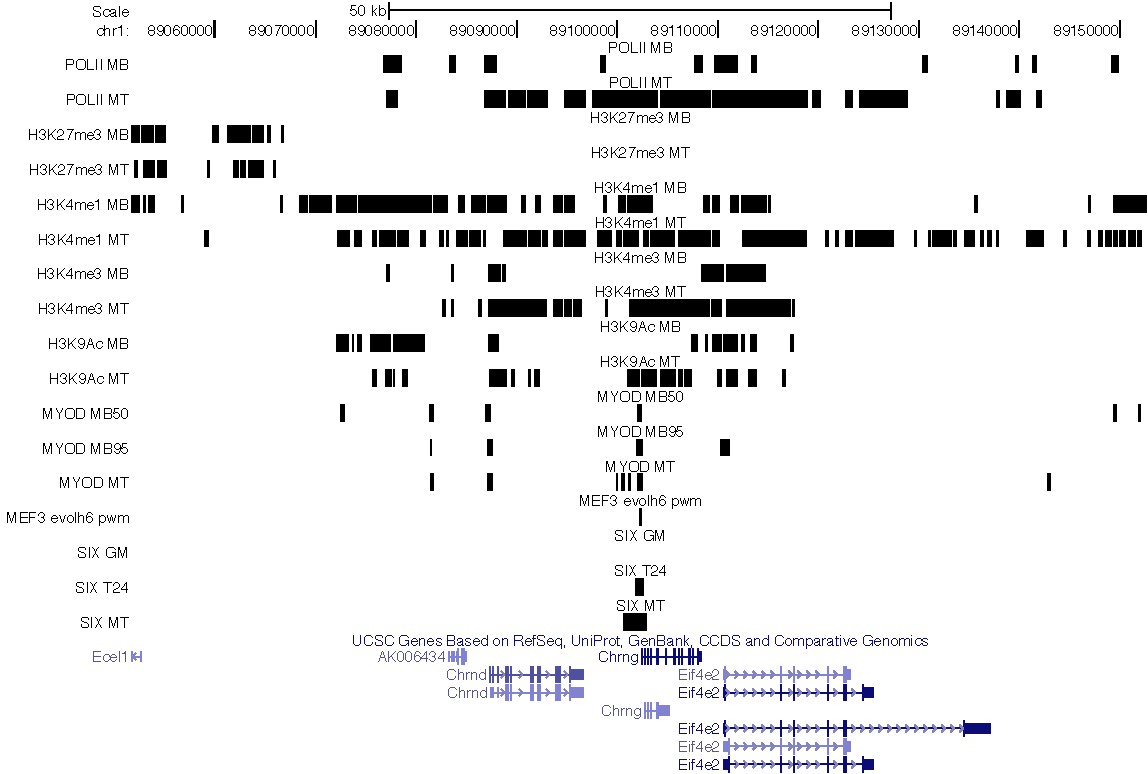
\includegraphics[width=1\textwidth]{figures/ucsc-chrng-view.pdf}
\captionbf{Visualisation de donn�es \chipseq \textit{via} le site UCSC}{

    La visualisation de diff�rentes donn�es \chipseq et bioinformatiques
    (bandes noires) permet de mettre en perspective le cas de la r�gulation de
    \textit{Chrng} (en bleu au bas de l'image) lors de la diff�renciation
    musculaire. Les donn�es \chipseq sont issues de la litt�rature et les
    donn�es bioinformatiques (MEF3) ont �t� obtenues au cours de cette th�se.
    Les rectangles noirs correspondent aux coordonn�es des pics obtenus apr�s
    avoir appliqu� un seuil de filtrage du bruit. Les donn�es de fixation de
    PolII ainsi que les donn�es de m�thylation et d'ac�tylation des histones
    (H3K4me$3$ et H3K9Ac, marques de l'activit� transcriptionnelle, voir
    fig.~\ref{fig:hardison-enhancer-states}), tir�es de \citet{Asp2011p2370},
    indiquent que le locus est transcrit lors de la formation de myotubes. Le
    TF MyoD est fix� au niveau du promoteur de \textit{Chrng} au cours de la
    prolif�ration des myoblastes (MB$50$, $50\%$ de confluence, et MB$95$,
    $95\%$ de confluence) et au cours de la diff�renciation en myotubes
    MT~\cite{Cao2010p1805}.  Le TF Six est co-fix� avec MyoD lors de la
    diff�renciation : � T$24$, $24$h apr�s diff�renciation, et
    � MT~\cite{Liu2010p588}. De plus, des analyses bioinformatiques montre
    l'existence dans cette r�gion d'un site de fixation MEF$3$ pour la prot�ine
    Six conserv� chez les vert�br�s, corroborant une liaison directe de l'ADN
    par Six. Prises ensemble, la simple visualisation de ces donn�es sugg�rent
    une r�gulation par Six et MyoD de \textit{Chrng}.

}
\label{fig:ucsc-chrng-view}
\efig

\subsection{Outils de visualisation}
\label{sub:outils_visualisation}

Afin d'avoir une id�e plus claire des �v�nements de r�gulation qui se d�roulent
� un locus donn�, il existe plusieurs outils de visualisation des annotations
g�nomiques et �pig�n�tiques, que ce soit sur le site du NCBI
(\url{http://www.ncbi.nlm.nih.gov/gene}), sur Ensembl ou sur UCSC Genome
Browser. Ce dernier poss�de notamment l'avantage qu'il est possible d'importer
des donn�es personnelles sous un grand nombre de formats, obtenues � partir de
la litt�rature ou � partir de ses propres travaux. Ainsi, nous pr�sentons en
figure \ref{fig:ucsc-chrng-view} quelques donn�es de \chipseq pour des TFs
musculaires et pour des marques �pig�n�tiques, ainsi que des pr�dictions
bioinformatiques de sites de fixation conserv�s pour les hom�oprot�ines Six
r�alis�e par nos soins. La visualisation sur UCSC Genome Browser permet de
rapidement d�terminer le mode de r�gulation putatif du g�ne \textit{Chrng}
: fixation de Six et MyoD au niveau du promoteur et apparition de marques
�pig�n�tiques H3K4me$1$ et H3Ac sur les histones au cours de la diff�renciation
de prog�niteurs musculaires.


Par ailleurs, il existe un outil de visualisation compl�mentaire de ceux cit�s
: le visualisateur de r�gions conserv�es au cours de l'�volution ECR Browser
(\url{http://ecrbrowser.dcode.org}), int�grant de nombreux outils
bioinformatiques~\cite{Loots2005ys}. Ce navigateur permet de visualiser la
conservation g�nomique d'un locus donn� chez plusieurs esp�ces plus ou moins
lointaines (par exemple souris, homme, vache, grenouille et poisson z�bre) afin
de cibler l'�tude de la r�gulation sur des r�gions extr�mement conserv�es. Il
est ensuite possible d'analyser les s�quences ultraconserv�es s�lectionn�es en
utilisant les motifs de la base de donn�e TRANSFAC \textit{via} l'outil
rVISTA~\cite{Loots2004vn}. Un exemple d'utilisation de cet outil est donn� par
la d�couverte de plusieurs r�gions de r�gulation fonctionnelles de
l'hom�oprot�ine Six1 poss�dant une extr�me conservation~\cite{Sato2012zr}.



\subsection{Le projet ENCODE}
\label{sub:projet_encode}

\bfig
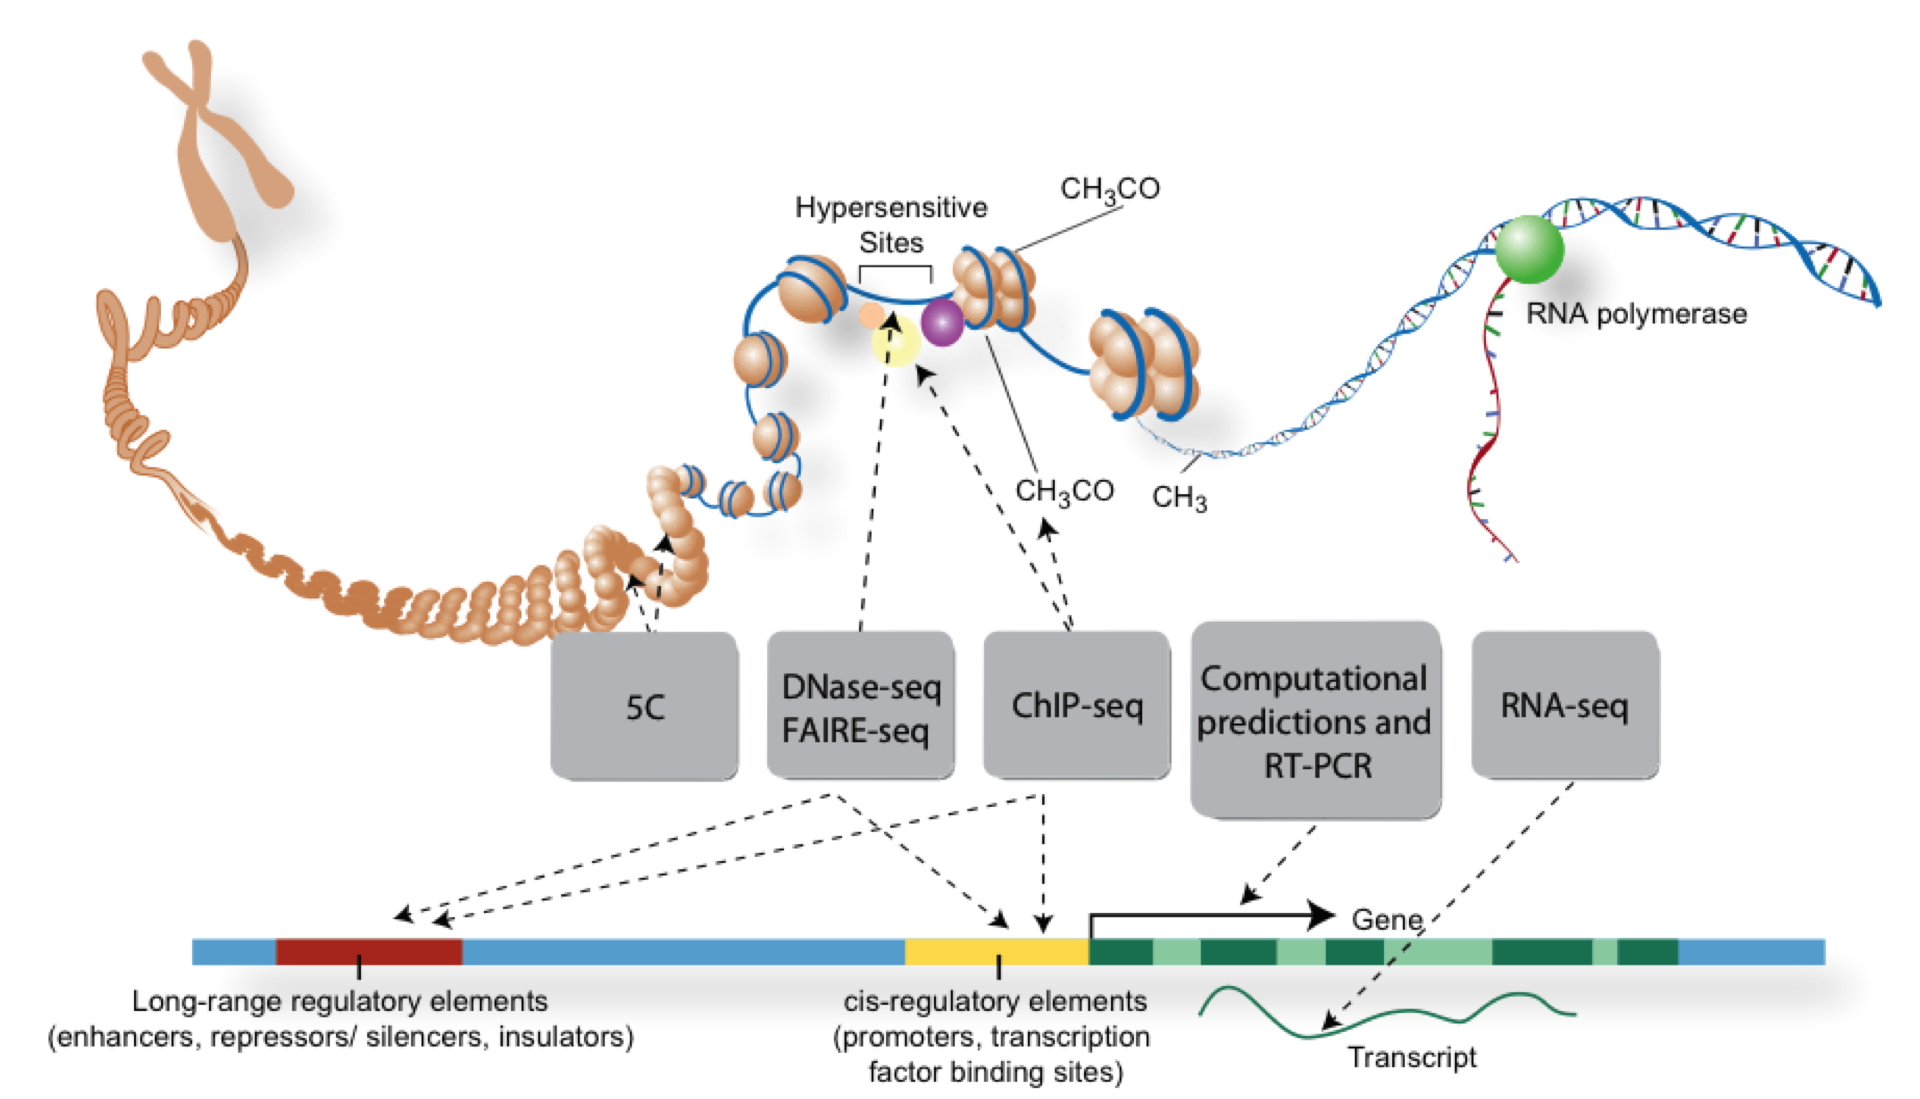
\includegraphics[width=1\textwidth]{figures/encode-workflow.png}
\captionbf{Les diff�rentes donn�es obtenues par le projet ENCODE}{

    Figure tir�e du site web du projet ENCODE
    (\url{http://genome.ucsc.edu/ENCODE}). Les �quipes associ�es � ce projet
    utilisent de multiples exp�riences et m�thodes pour identifier les �l�ments
    fonctionnels du g�nome. L'annotation des g�nes se fait principalement par
    le s�quen�age de l'ARN provenant de diff�rentes sources (tissu, stade de
    d�veloppement), la g�nomique comparative, des m�thodes bioinformatiques ou
    encore par annotation manuelle. Les �l�ments de r�gulation sont quant � eux
    �tudi�s \textit{via} des exp�riences d'hypersensibilit� � la DNAseI,
    l'�tude de la m�thylation de l'ADN, ou encore les donn�es \chipseq de
    divers \tfs et histones sp�cifiquement m�thyl�es ou ac�tyl�es.

}
\label{fig:encode-workflow.png}
\efig

Le projet ENCODE (pour \textit{Encyclopedia of DNA Elements}) est un consortium
de groupes de recherche internationaux financ�s par le NHGRI (\textit{National
Human Genome Research Institute}) qui a vu le jour afin de syst�matiser les
m�thodes permettant l'annotation des g�nomes et de faciliter l'int�gration des
nombreuses donn�es obtenues. Son but est de construire une liste exhaustive des
�l�ments fonctionnels du g�nome humain, qu'ils agissent au niveau de l'ADN, de
l'ARN ou des prot�ines, et des �l�ments de r�gulation qui contr�lent l'�tat
cellulaire et l'activit� des g�nes. Les donn�es sont mises � disposition du
public gratuitement sur internet (\url{http://genome.ucsc.edu/ENCODE/}).
� noter que des projets �quivalents existent pour d'autres organismes, comme la
souris (\url{http://mouseencode.org}), ou encore le ver \celegans et la mouche
\dmel (\url{http://www.modencode.org}).


Totalisant en septembre $2012$ plus de $1600$ exp�riences dans plus de $147$
types cellulaires, les premi�res conclusions pointent vers une profusion
d'�v�nements de r�gulation, loin de l'id�e d'ADN poubelle (\textit{junk DNA})
: ainsi, $80\%$ du g�nome est associ� � un �v�nement biochimique associ� � de
la formation d'ARN ou au remodelage de la chromatine, $\sim400,000$ r�gions
poss�dent un �tat chromatinien caract�ristique des enhancers et $\sim70,000$
des promoteurs~\cite{ENCODE-Project-Consortium2012ly}. Depuis mai 2013, les
donn�es \chipseq de $161$ TFs couvrant $91$ types cellulaires ont �t� mises
� disposition sur UCSC Genome
Browser\footnote{\url{http://genome.ucsc.edu/cgi-bin/hgTrackUi?db=hg19&g=wgEncodeAwgTfbsUniform}}.


%\bfig
%
\includegraphics[width=0.8\textwidth]{figures/siggia-fate.pdf}
%\captionbf{Vision g�om�trique des transitions entre types cellulaire}{
%   Figure tir�e de \cite{Corson2012p3973} sch�matisant le processus de
%   diff�renciation des cellules de la vulve de \celegans.
%   \textbf{A.} La cellule est dans un �tat pr�curseur repr�sent� par une
%   bille au fond d'une vall�e.
%   \textbf{B.} La cellule est dans �tat dit \textit{comp�tent} o� elle peut basculer
%   vers diff�rents destins cellulaires.
%   \textbf{C.} Un signal externe repr�sent� par une fl�che rouge modifie le
%   paysage de mani�re � favoriser l'un des �tats finaux possibles.
%} 
%\efig

%\bfig
%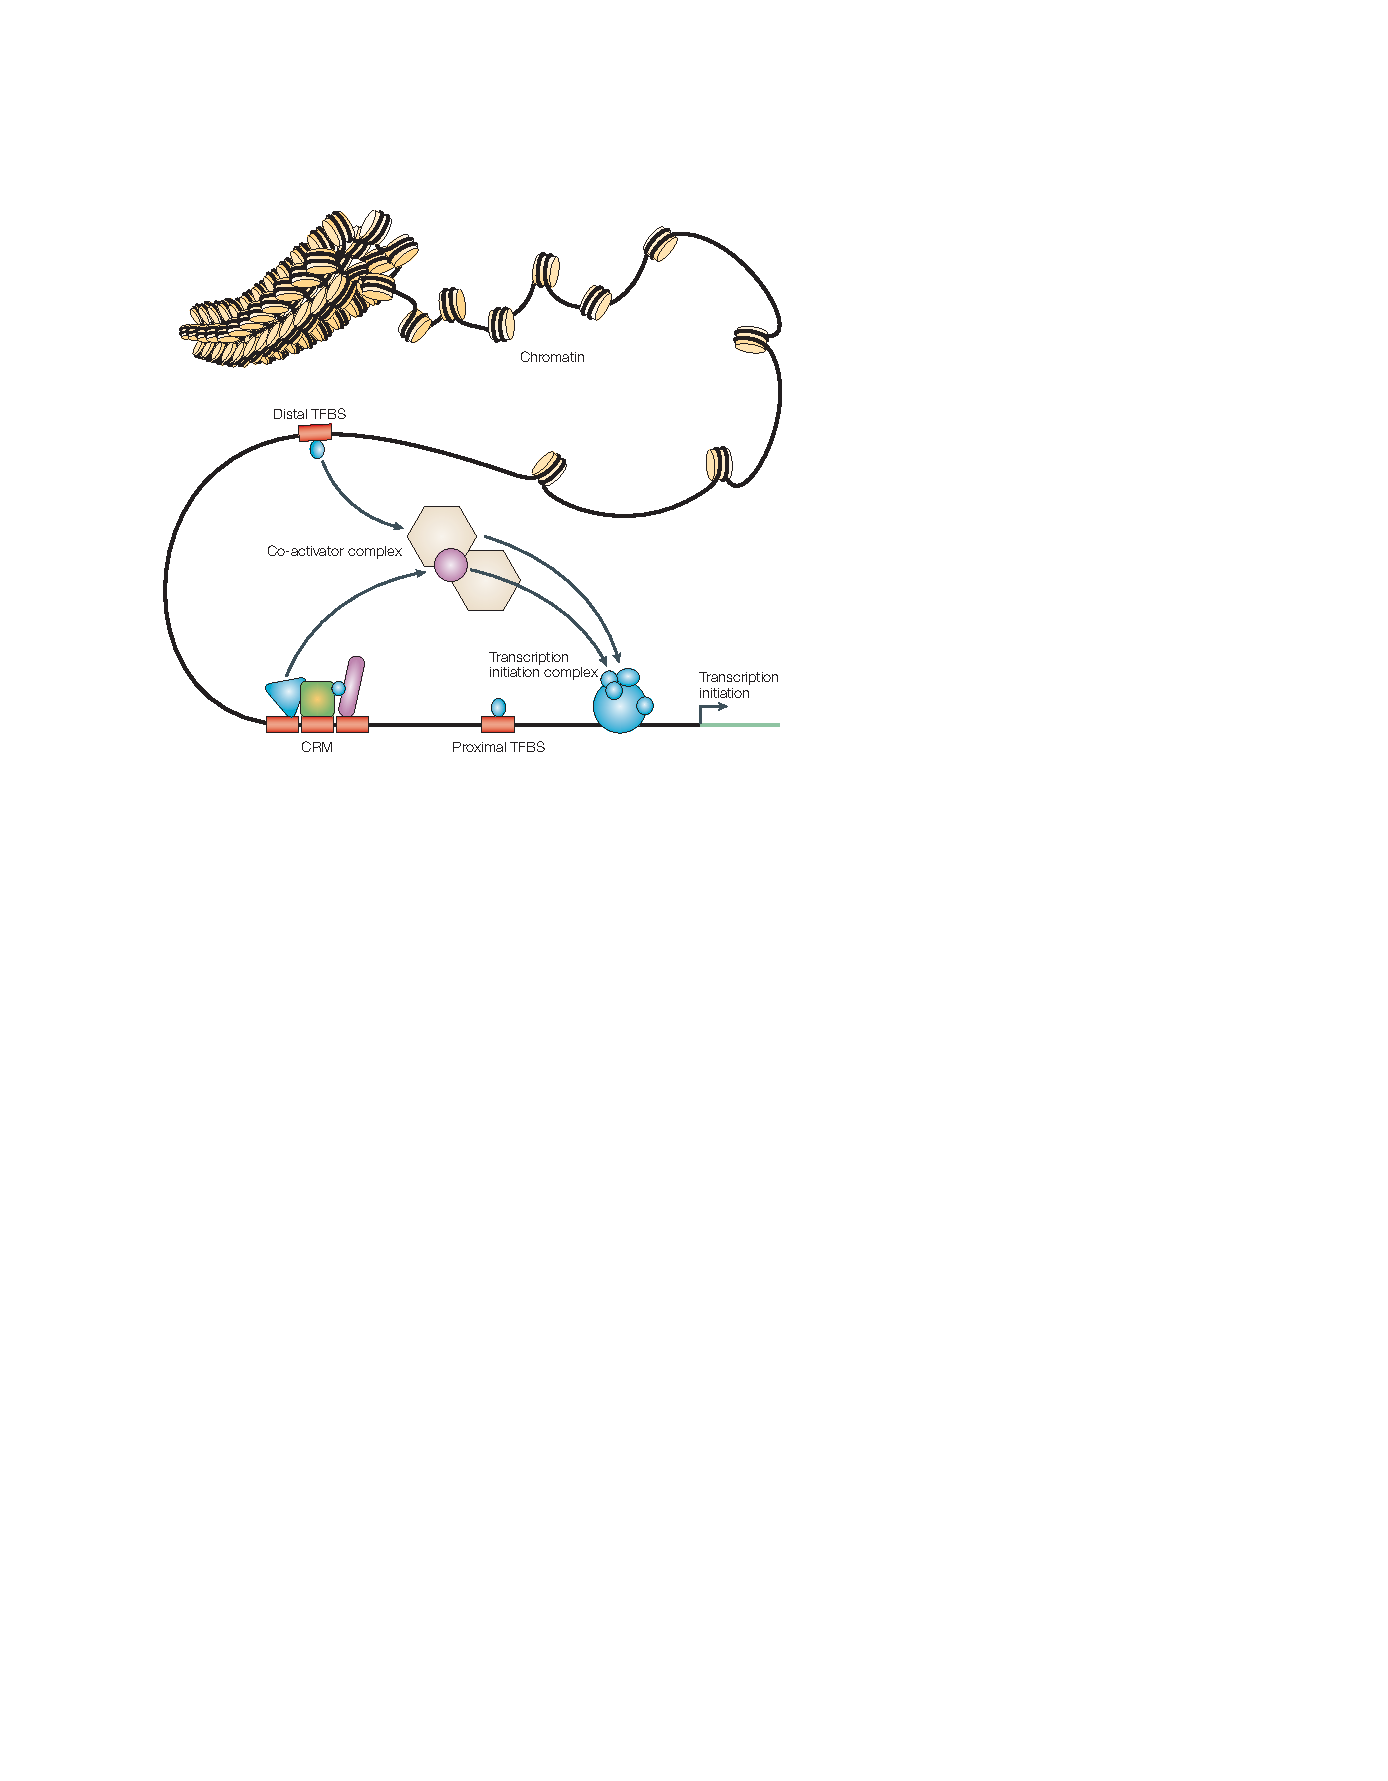
\includegraphics[width=.8\textwidth]{figures/wasserman-transcriptional-regulation.pdf}
%\captionbf{Les diff�rentes composantes de la r�gulation transcriptionnelle}{
    %Figure tir�e de \cite{Wasserman2004p624}. Les \TFs se fixent � des sites
    %sp�cifiques de longueur $\sim10$bp qui peuvent �tre proximaux (promoteur,
    %premiers introns) ou distaux (plus de $100$kb) d'un \TSS. Diff�rents \TFs
    %peuvent s'assembler sur des r�gions d'ADN de taille typique $\sim 1000$bp
    %appel�es \CRMs afin de conduire � une r�gulation sp�cifique, par simple
    %effet de communaut� par exemple lorsque la fixation de tous les \tfs est
    %requise pour que la r�gulation op�re. Les interactions entres les \tfs et
    %diff�rents cofacteurs stabilisent la machinerie d'initiation de
    %transcription pour permettre l'expression g�n�tique. La r�gulation distale
    %est quant � elle fortement d�pendante de la structure tridimensionnelle de
%la chromatine.  } \efig


\newpage 

%%%%%%%%%%%%%%%%%%%%%%%%%%%%%%%%%%%%%%%%%%%%%%%%%%%%%%%%%%%%%%%%%%%%%%%%%%%%%%%%%%%%%%%%%%
\chapter{\ChMaxent} 
\label{ch:maxent}
%\adjustmtc
\minitoc
\newpage
\section*{Introduction du chapitre \thechapter}

Dans cette partie, nous nous int�ressons � la description de l'interaction
entre les \fts et leurs sites de reconnaissance sur l'ADN.  Pendant longtemps,
la qualit� de cette description a �t� limit�e par la quantit� de donn�es
disponibles. Ainsi, les exp�riences de type SELEX (voir
\ref{sub:approches_invitro}), o� des exp�riences de \chip au cas par cas
permettaient de r�cup�rer de l'ordre de quelques dizaines de sites de fixation
pour un TF d'int�r�t. Or, le mod�le PWM, qui est le mod�le le plus simple (en
terme de nombre de param�tres) que l'on puisse b�tir pour d�crire l'interaction
poss�de d�j� plusieurs dizaines de param�tres -- les fr�quences des nucl�otides
� chaque position --. 

Ces donn�es ne permettaient donc pas d'explorer plus en avant des mod�les plus
complexes de fixation incluant par exemple des termes d'interaction entre
nucl�otides au sein des sites de fixation. Cependant, les avanc�es r�centes en
s�quen�age � haut d�bit ont permis l'obtention de donn�es tr�s grande �chelle,
que ce soit \invivo par \chipseq ou \invitro par HT-SELEX (voir
\ref{sec:mesures_exp}). Le nombre de sites de fixation obtenus est de l'ordre
de quelques milliers, ce qui permet de contraindre des mod�les de fixation plus
complexe que le mod�le PWM.

En utilisant des donn�es \chipseq pour un grand nombre de \fts de la Drosophile
et des vert�br�s, nous avons contraint diff�rents mod�les de fixation incluant
implicitement ou explicitement des interactions entre nucl�otides. Nous les
avons compar�s sur leur capacit� � d�crire les statistiques de fixation TF-ADN
observ�es \invivo. Nous pr�sentons pr�alablement un survol des observations et
mod�les existant au sujet des corr�lations dans les sites de fixations de \fts.

\section{Observations de corr�lations au sein des TFBS}
\label{sec:corr_lations_au_sein_des_sites_de_fixation_de_tfs}

Diff�rents travaux ont mis en exergue l'existence de corr�lations entre
nucl�otides au sein des sites de fixation de TFs. Parce que limit�es par la
quantit� de donn�es alors possible � obtenir, les premi�res �tudes de ce genre
ont centr� leur attention sur quelques corr�lations importantes pour des cas
particuliers. Ainsi, \citet{Man2001fk} ont observ� que la prot�ine Mnt induit
des corr�lations entre les positions $16$ et $17$ de ses sites de
reconnaissance \invitro. Ils ont mesur� exp�rimentalement la sp�cificit� aux
sites de liaisons contenant tous les variants possibles � ces deux positions.
Ils ont ainsi observ� que la mutation de la base consensus C en position 17
induisait un changement de pr�f�rence en position 16 de la base A vers la base
C. Par ailleurs, \citet{Bulyk2002uq} ont montr� que la prot�ine EGR$1$ induisait
des corr�lations au sein d'un triplet de nucl�otides central de leur site de
reconnaissance. La prise en compte de ces corr�lations dans l'�nergie de
fixation permettait alors d'am�liorer la description des donn�es par rapport au
mod�le additif PWM.

� une plus grande �chelle, \citet{Badis2009p3911} ont utilis� des puces � ADN
(technique PBM, cf \ref{sub:approches_invitro}) pour �tudier la fixation
\invitro de $104$ TFs de la souris sur toutes les s�quences d'ADN de $10$ bp
possibles. Pour chaque facteur, plusieurs centaines de s�quences de fixation
ont ainsi �t� obtenues. L'�tude a r�v�l� l'existence d'une multiplicit� de
motifs (PWMs) pour la plupart des TFs (seulement $15$ �tant mieux d�crit par un
motif unique). Certains motifs reconnaissent notamment des s�quences
� espacement variable pour lesquelles deux r�gions sp�cifiques du site sont
s�par�es par un nombre variable de nucl�otides. Enfin, les auteurs ont not� la
pr�sence de corr�lations fortes dans $19$ cas, celles-ci n'�tant pas forc�ment
limit�es � des dinucl�otides mais pouvant impliquer des trinucl�otides. Plus
r�cemment, \citet{Jolma2013p3971} ont analys� par HT-SELEX plusieurs centaines
de domaines de fixations � l'ADN de TFs humains et de la souris, r�v�lant aussi
l'importance d'espacements variables et surtout des corr�lations
dinucl�otidiques entre plus proches voisins.


\section{Mod�les existants permettant de d�crire la statistique des TFBS}
\label{sec:mod_les_pour_d_crire_les_corr_lations}

Diff�rents mod�les ont �t� propos�s pour d�crire ces corr�lations
(fig.~\ref{fig:modeles-correlations}). La m�thode la plus directe consiste
� partir du mod�le PWM (fig.~\ref{fig:modeles-correlations}a) et � ajouter des
corr�lations mutuellement exclusives aux positions les plus corr�l�es
(fig.~\ref{fig:modeles-correlations}b). D'autres m�thodes utilisent des
structures probabilistes de d�pendances sous forme de cha�nes de Markov
(fig.~\ref{fig:modeles-correlations}c) ou plus g�n�ralement de r�seau bay�sien
(fig.~\ref{fig:modeles-correlations}d-e). Enfin, une derni�re m�thode consiste
� r�aliser des m�langes de mod�les afin de capturer des ensembles distincts de
corr�lations (fig.~\ref{fig:modeles-correlations}f-g).

\bfig
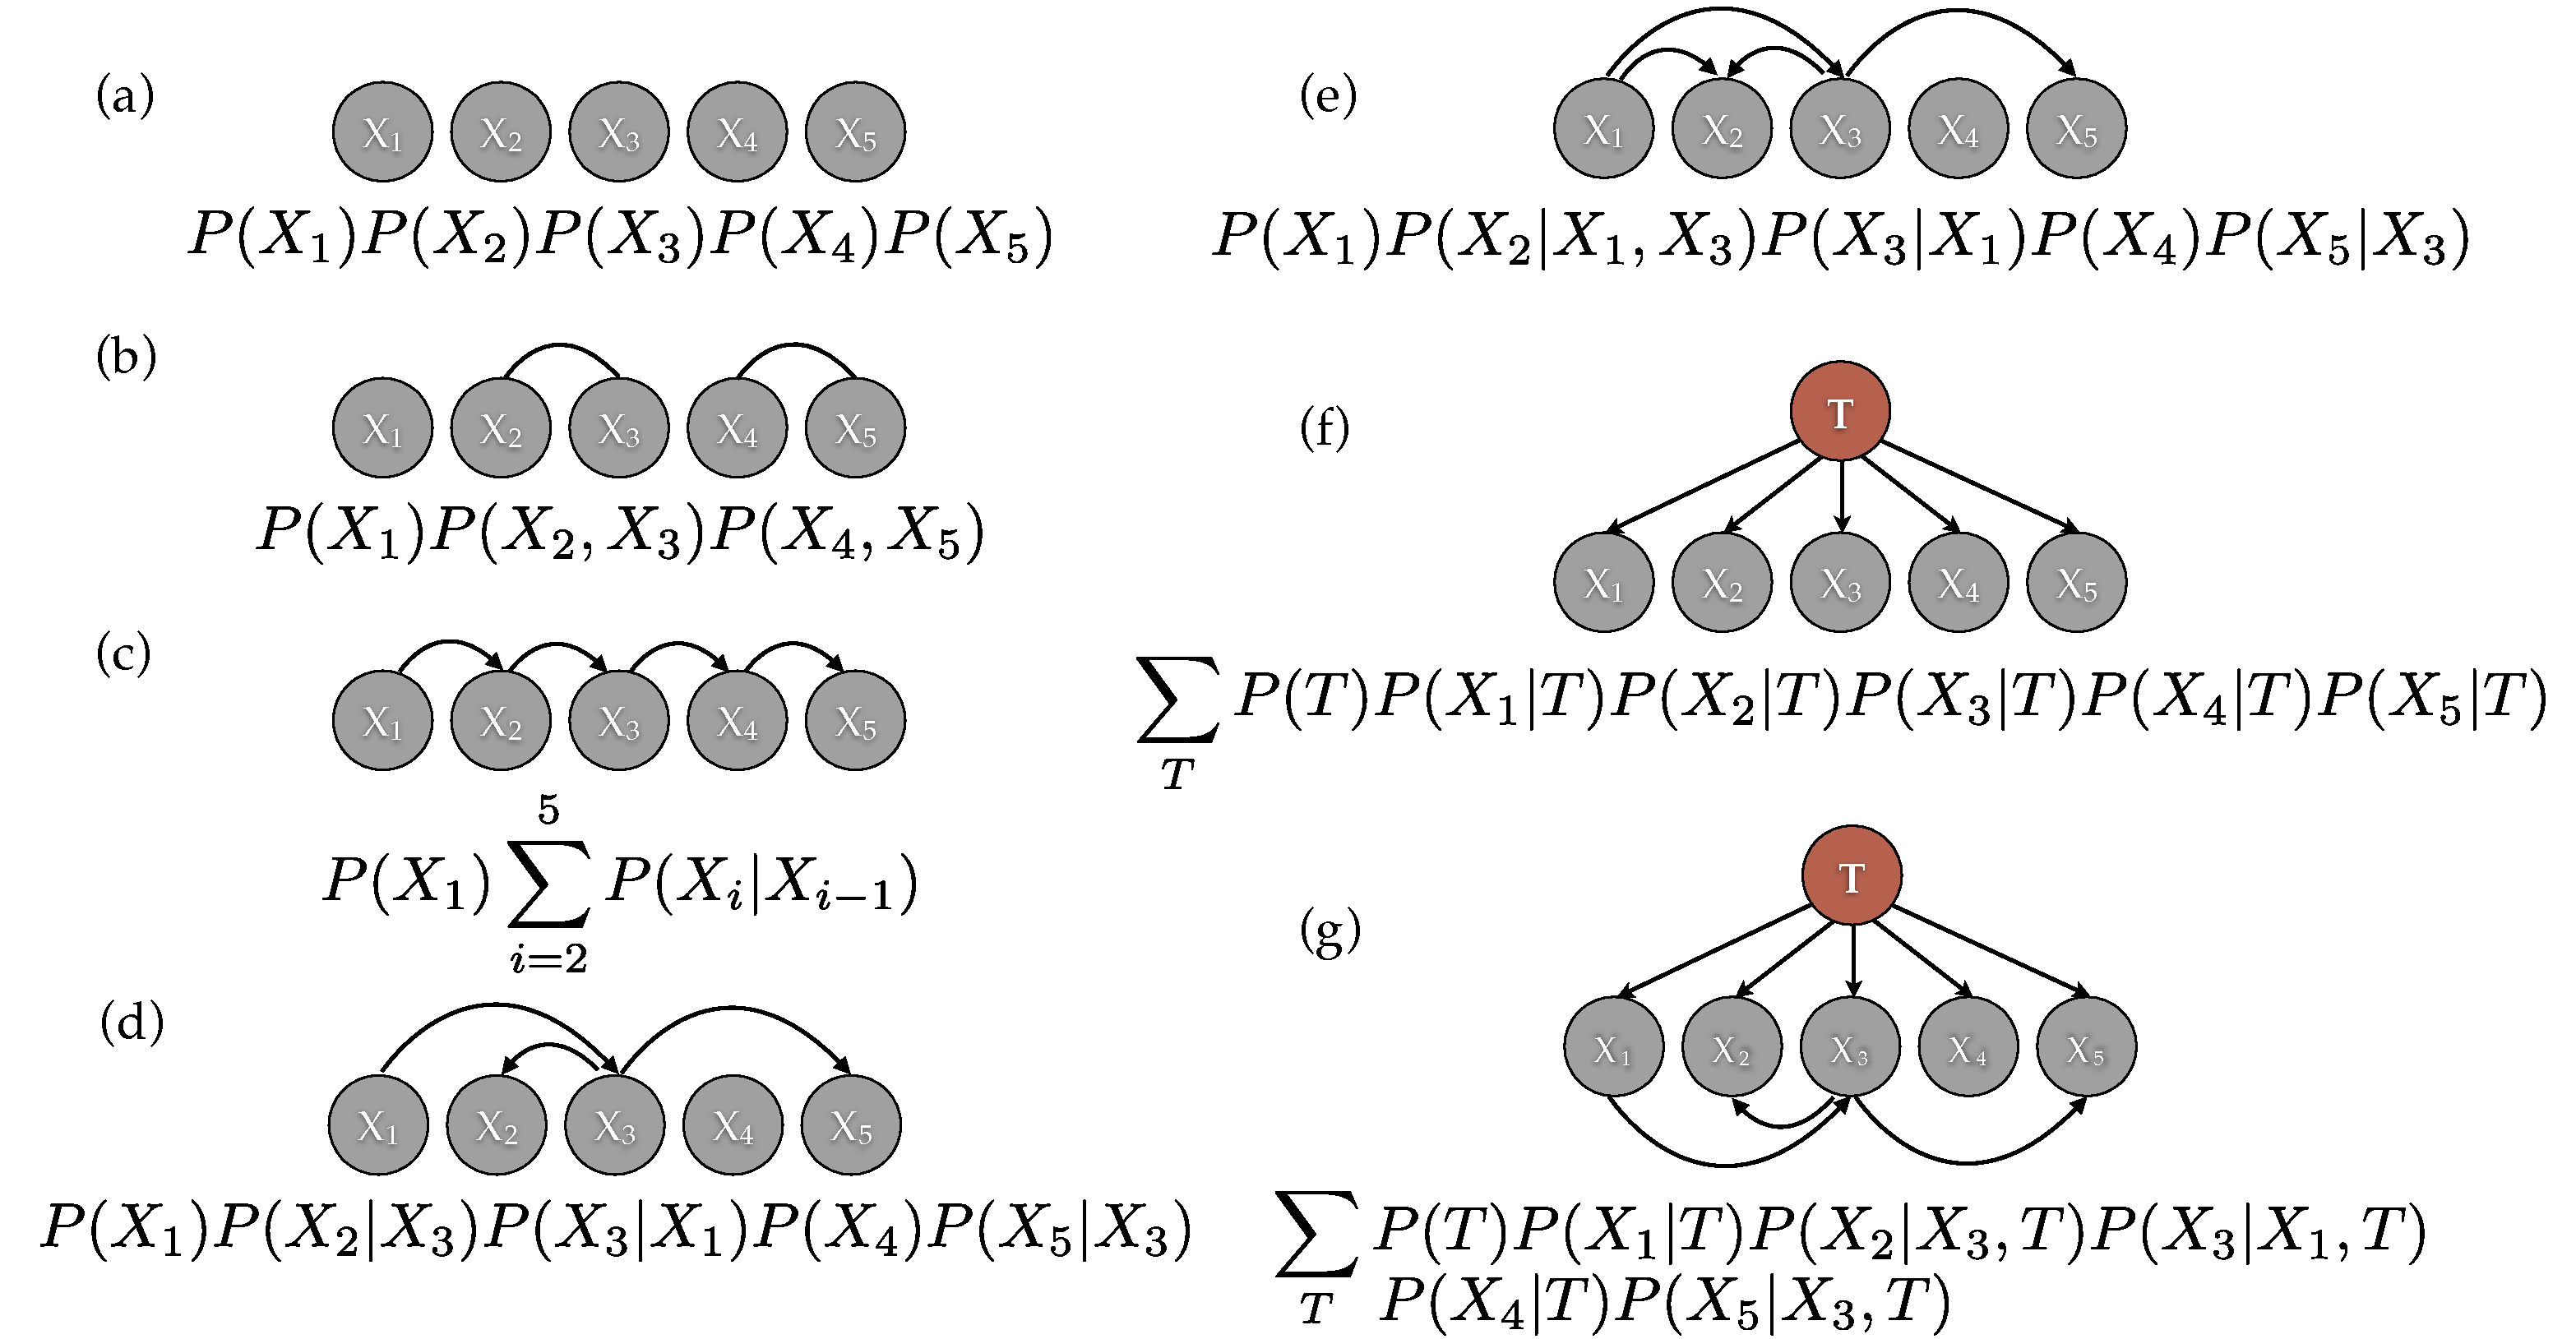
\includegraphics[width=1\textwidth]{figures/modeles-correlations.pdf}
\captionbf{Diff�rents mod�les pour d�crire les corr�lations entre nucl�otides dans les sites de fixation de \fts}{

    Figure adapt�e de \citet{Barash2003MDP} illustrant diff�rents mod�les de
    fixation sur un site de longueur $5$. Pour chaque mod�le, la structure du
    r�seau de d�pendances sous-jacent est repr�sent�e, ainsi que la
    distribution de probabilit� $P(X_1,X_2,X_3,X_4,X_5)$ correspondante, o�
    $X_i$ est une variable al�atoire prenant la valeur (A, C, G ou T) du
    nucl�otide � la position $i$.  Les mod�les repr�sent�s sont les suivants
    : (a) PWM (pas de corr�lations), (b) GWM (corr�lations mutuellement
    exclusives), (c) cha�ne de Markov d'ordre $1$ (corr�lations entre plus
    proches voisins), (d) r�seau bay�sien en arbre (au plus un parent par
    n{\oe}ud) ou (e) pas en arbre (le n{\oe}ud $2$ a deux parents), (f) m�lange
    de PWMs et (e) m�lange d'arbres � d�pendances fix�es.

}
\label{fig:modeles-correlations}
\efig

\subsection{Mod�le de r�f�rence sans corr�lations : la PWM}
\label{sub:mod_le_de_r_f_rence_sans_corr_lations_la_pwm}

Nous l'avons vu, le mod�le le plus simple (en termes de nombre de param�tres)
d�crivant l'interaction entre un TF et son site de reconnaissance sur l'ADN
consiste � faire l'hypoth�se que les nucl�otides contribuent ind�pendamment
� l'�nergie de fixation. Cette hypoth�se conduit au mod�le PWM (section
\ref{sub:modele_pwm} et fig.\ref{fig:modeles-correlations}a), qui s'�crit
\footnote{ 
    Comme nous l'avons signal� en \ref{sub:modele_pwm}, le terme PWM
    (\textit{Position Weight Matrix}) r�f�re en fait � la matrice des poids
    $\log(P(X_i)/\pi_{X_i})$ o� $\pi_{X_i}$ est une distribution neutre
    ind�pendante de la position (dite distribution \textit{background}), par exemple calcul�e
    sur des r�gions interg�niques.  
} :

\begin{equation}
    P(X_1,\cdots,X_k) = \prod_{i=1}^{K} P(X_i)
\end{equation}

o� $P(X_i)$ est la probabilit� marginale d'observer le nucl�otide $X \in
\{A,C,G,T\}$ � la position $i$. Un tel mod�le poss�de $3K$ param�tres -- $3$
param�tres $P(X_i)$ par position, la normalisation des probabilit�s permettant
de fixer le param�tre restant --. Pour une longueur de site typique $K=10$, le mod�le
PWM contient $30$ param�tres � contraindre, sachant qu'un \og mod�le \fg
complet param�trant la distribution jointe sans faire d'hypoth�se comporterait
$4^{10}-1 \sim 10^6$ param�tres.

% subsection mod_le_de_r_f_rence_sans_corr_lations_la_pwm (end)

\subsection{Une PWM g�n�ralis�e : le mod�le GWM}
\label{sub:mod_lisation_de_corr_lations_mutuellement_exclusives_le_mod_le_gwm}

 Une premi�re m�thode permettant de complexifier le mod�le PWM consiste
 � int�grer explicitement des groupes mutuellement exclusif 
 \footnote{
 Les corr�lations entre des couples de positions (i,j) et (j,k) ne peuvent �tre
 admises au sein du m�me mod�le.
 }
 de nucl�otides corr�l�s au sein du mod�le
 (fig.~\ref{fig:modeles-correlations}b). Une telle m�thode fut d'abord employ�e
 par \citet{Benos2002p3912} pour prendre en compte des corr�lations
 pr�alablement d�finies entre nucl�otides plus proches voisins. De mani�re plus
 g�n�rale, \citet{zhou2004modeling} ont d�velopp� un mod�le de matrice de poids
 g�n�ralis�e (GWM pour \textit{Generalized Weight Matrix}) qui prend en compte
 de mani�re syst�matique les corr�lations permettant d'am�liorer le mod�le
 ind�pendant. Pour ce faire, les auteurs utilisent une m�thode de Monte-Carlo
 par cha�ne de Markov (MCMC) : des corr�lations sont ajout�es ou enlev�es au
 hasard au mod�le et accept�es selon la r�gle de
 Metropolis-Hastings~\cite{krauth2006statistical}. Cette acceptation est
 proportionnelle au facteur de Bayes, une quantit� qui permet de comparer des
 mod�les poss�dant des nombres de param�tres diff�rent 
 \footnote{ 
     Sous certaines approximation, ce facteur peut se rapporter � une
     diff�rence de valeurs du BIC, introduit dans l'article en
     \ref{sec:article_maxent}. 
 } 
 .  
 Ce facteur est d�fini par le rapport entre la probabilit� de g�n�rer les
 donn�es $D$ (les s�quences de fixation) avec un mod�le $M_1$ de param�tres
 $\theta_1$ plut�t qu'avec un autre mod�le $M_2$ de param�tres $\theta_2$ :

\begin{equation}
    BF = \frac{P(D|M_1)}{P(D|M_2)} = \frac{\int P(D | \theta_1, M_1) P(\theta_1|M_1) d\theta_1}{\int P(D | \theta_2, M_2) P(\theta_2|M_2) d\theta_2}
\end{equation}

Le mod�le final consiste en un ensemble de param�tres d�crivant des positions
ind�pendantes et des positions corr�l�es mutuellement exclusives .  En analysant les donn�es TRANSFAC, les auteurs ont not� que
dans $25\%$ des cas ($22/95$) le mod�le GWM �tait significativement meilleur
que le mod�le PWM (facteur de Bayes sup�rieur � $6$). 


Cette m�thode a par la suite �t� utilis�e sur des donn�es \chipseq pour $4$ TFs
mammif�res -- NRSF, STAT$1$, CTCF et ER --~\cite{hu2010detection}. En utilisant
les $10\%$ des pics les plus importants comme ensemble d'apprentissage et en se
restreignant aux r�gions de $200$bp centr�es autour du sommet du pic \chip, les
auteurs ont r�alis� un �chantillonnage de Gibbs~\cite{casella1992explaining}
pour obtenir les sites de fixation suivant les hypoth�ses que (1) chaque pic
contient au plus un seul site de fixation (mod�le ZOOPS pour \textit{Zero or
One Occurrences Per Sequence}), (2) la probabilit� \apriori d'avoir un site
� une certaine position sur la s�quence est plus forte autour du sommet du pic,
et (3) les sites sont d�crits par un mod�le GWM.  L'�tude a r�v�l� l'existence
de corr�lations fortes limit�es aux nucl�otides plus proches voisins dans les
quatre cas �tudi�s. Les nucl�otides participant aux corr�lations se situaient
� des positions ayant un faible contenu en information dans le mod�le PWM.
Enfin, les auteurs ont not� la pr�sence de plusieurs triplets de nucl�otides
voisins corr�l�s.

% subsection mod_lisation_de_corr_lations_mutuellement_exclusives_le_mod_le_gwm (end)


\subsection{R�seaux bay�siens}
\label{sub:r_seaux_bay_siens}

Une g�n�ralisation du mod�le GWM consiste � supprimer la condition d'exclusion
mutuelle des paires de nucl�otides corr�l�s en d�crivant de mani�re plus
g�n�rale le r�seau de d�pendance entre positions. Une telle description est
possible en utilisant le langage des r�seaux bay�siens. Les d�pendances y sont
repr�sent�es par un graphe orient� acyclique \footnote{ Un graphe orient�
    acyclique est un r�seau dont les liens sont orient�s et au sein duquel il
    n'est pas possible de revenir � son point de d�part en suivant les fl�ches
} $G$, dont les n{\oe}uds sont les variables $X_i$ et les liens repr�sentent
les conditionnements d'une variable avec des variables parentes
(fig.~\ref{fig:modeles-correlations}e). La probabilit� jointe s'�crit :

\begin{equation}
    P(X_1,\cdots,X_k) = \prod_{i=1}^{K} P(X_i | P_i^G)
\end{equation}

o� $P_i^G$ est l'ensemble (pouvant �tre vide) des parents de $X_i$ dans $G$. Le
nombre de param�tres peut rapidement devenir grand : si l'on note $N_i$ le
nombre de parents de $X_i$, alors le nombre de param�tres du mod�le est $3
\sum_{i=1}^K 4^{N_i}$.

Lorsque les diff�rents n{\oe}uds poss�dent au plus un parent, on parle d'arbre
bay�sien (fig.~\ref{fig:modeles-correlations}d). Ce type de r�seau bay�sien
g�n�ralise notamment le cas des cha�nes de Markov d'ordre $1$, o� chaque
n{\oe}ud d�pend du n{\oe}ud pr�c�dent (fig.~\ref{fig:modeles-correlations}c).
Le nombre de param�tres est alors restreint, puisqu'il est au plus de
$3\cdot4K$.  \\

L'avantage des arbres bay�siens est qu'il existe des algorithmes efficaces
permettant de trouver la meilleure structure
d'arbre~\cite{friedman1997bayesian}. De tels mod�les d'arbres ont �t� utilis�s
pour d�crire les donn�es de $95$ TFs de Transfac~\cite{Barash2003MDP}. Dans
$\sim25\%$ des cas ($22/95$), le mod�le d'arbre bay�sien s'av�re
significativement meilleur qu'un mod�le PWM, ce qui est du m�me ordre de
grandeur que pour le mod�le GWM vu
en~\ref{sub:mod_lisation_de_corr_lations_mutuellement_exclusives_le_mod_le_gwm}.


% subsection r_seaux_bay_siens (end)

\subsection{Mod�les de m�lange}
\label{sub:mod_les_de_m_lange}

Dans les cas pr�c�dents, nous avons pr�sent� des mod�les capturant des
d�pendances \og locales \fg entre paires de nucl�otides. N�anmoins, il peut
exister des d�pendances plus largement r�parties entre les positions, comme
cela a d�j� �t� observ� empiriquement~\cite{Badis2009p3911,Jolma2013p3971}. De
telles corr�lations � plus grande �chelle peuvent �tre mod�lis�es en supposant
que le \tf poss�de plusieurs \og modes \fg de fixation. Ceux-ci peuvent par
exemple correspondre � diff�rentes conformations de la prot�ine sur son site de
fixation, chaque configuration poss�dant ses propres pr�f�rences de fixation.
Ces modes sont d�crits par une variable al�atoire $T$ (le \textit{type} de
fixation) de probabilit� $P(T)$. Il est ensuite possible de d�crire la fixation
au sein de chaque mode par l'un des mod�les pr�c�dents.

\subsubsection{M�lange de PWMs}
\label{ssub:m_lange_de_pwms}

Le cas le plus naturel consiste � utiliser comme mod�le de fixation le mod�le
PWM, \cad que dans chaque mode il y a ind�pendance entre les positions. La
probabilit� d'observer un site est alors donn�e par la somme sur les diff�rents
modes de fixation de la probabilit� de fixer un site, conditionn�e par la
probabilit� d'�tre dans ce mode :

\begin{equation}
    P(X_1,\cdots,X_K) = \sum_{T=1}^N P(T) \prod_{i=1}^K P(X_i|T)
\end{equation}

o� $N$ est le nombre de modes de fixation. Ce mod�le a plusieurs avantages.
D'abord, le nombre de param�tres reste lin�aire en $K$ : pour d�crire $P(T)$ et
les $N$ PWMs il faut $N - 1 + 3KN$ param�tres. Ce nombre reste dont
raisonnablement faible devant le nombre de param�tres requis pour compl�tement
d�crire les interactions � deux nucl�otides, qui cro�t comme $K^2$. Ensuite, le
mod�le a une interpr�tation claire qui peut permettre de mettre en exergue un
m�canisme biologique sous-jacent.  \\

Ce type de mod�le permet de d�passer le mod�le PWM dans un nombre substantiel
de cas. Ainsi, \citet{Barash2003MDP} ont montr� que $\sim40\%$ des TFs de
Transfac ($36/95$) sont significativement mieux repr�sent�s par un m�lange de
$2$ PWMs que par une seule PWM. En utilisant des donn�es \invitro plus pr�cises
pour $104$ TFs de la souris, \citet{Badis2009p3911} ont montr� que $\sim 85\%$
($89/104$) �taient mieux repr�sent� par une combinaison de PWMs que par une PWM
seule, plaidant pour un port�e g�n�rale de l'existence de \og motifs
secondaires \fg.


% subsubsection m_lange_de_pwms (end)


\subsubsection{M�lange d'arbres}
\label{ssub:m_lange_d_abres}

De la m�me mani�re que les PWMs, il est possible d'�tendre les mod�les d'arbres
en r�alisant un m�lange d'arbres. Intuitivement, ceci permet de capturer des
d�pendances additionnelles en gardant un nombre de param�tres lin�aire en
fonction de la taille du motif. Un tel mod�le semble poss�der des performances
comparables au m�lange de PWM, et am�liore la description des TFs de Transfac
dans $\sim40\%$ des cas ($35/95$)~\cite{Barash2003MDP}.


% subsubsection m_lange_d_abres (end)


% subsection mod_les_de_m_lange (end)

\section{Mod�les de maximum d'entropie}
\label{sec:modeles-maxent}

\bfig
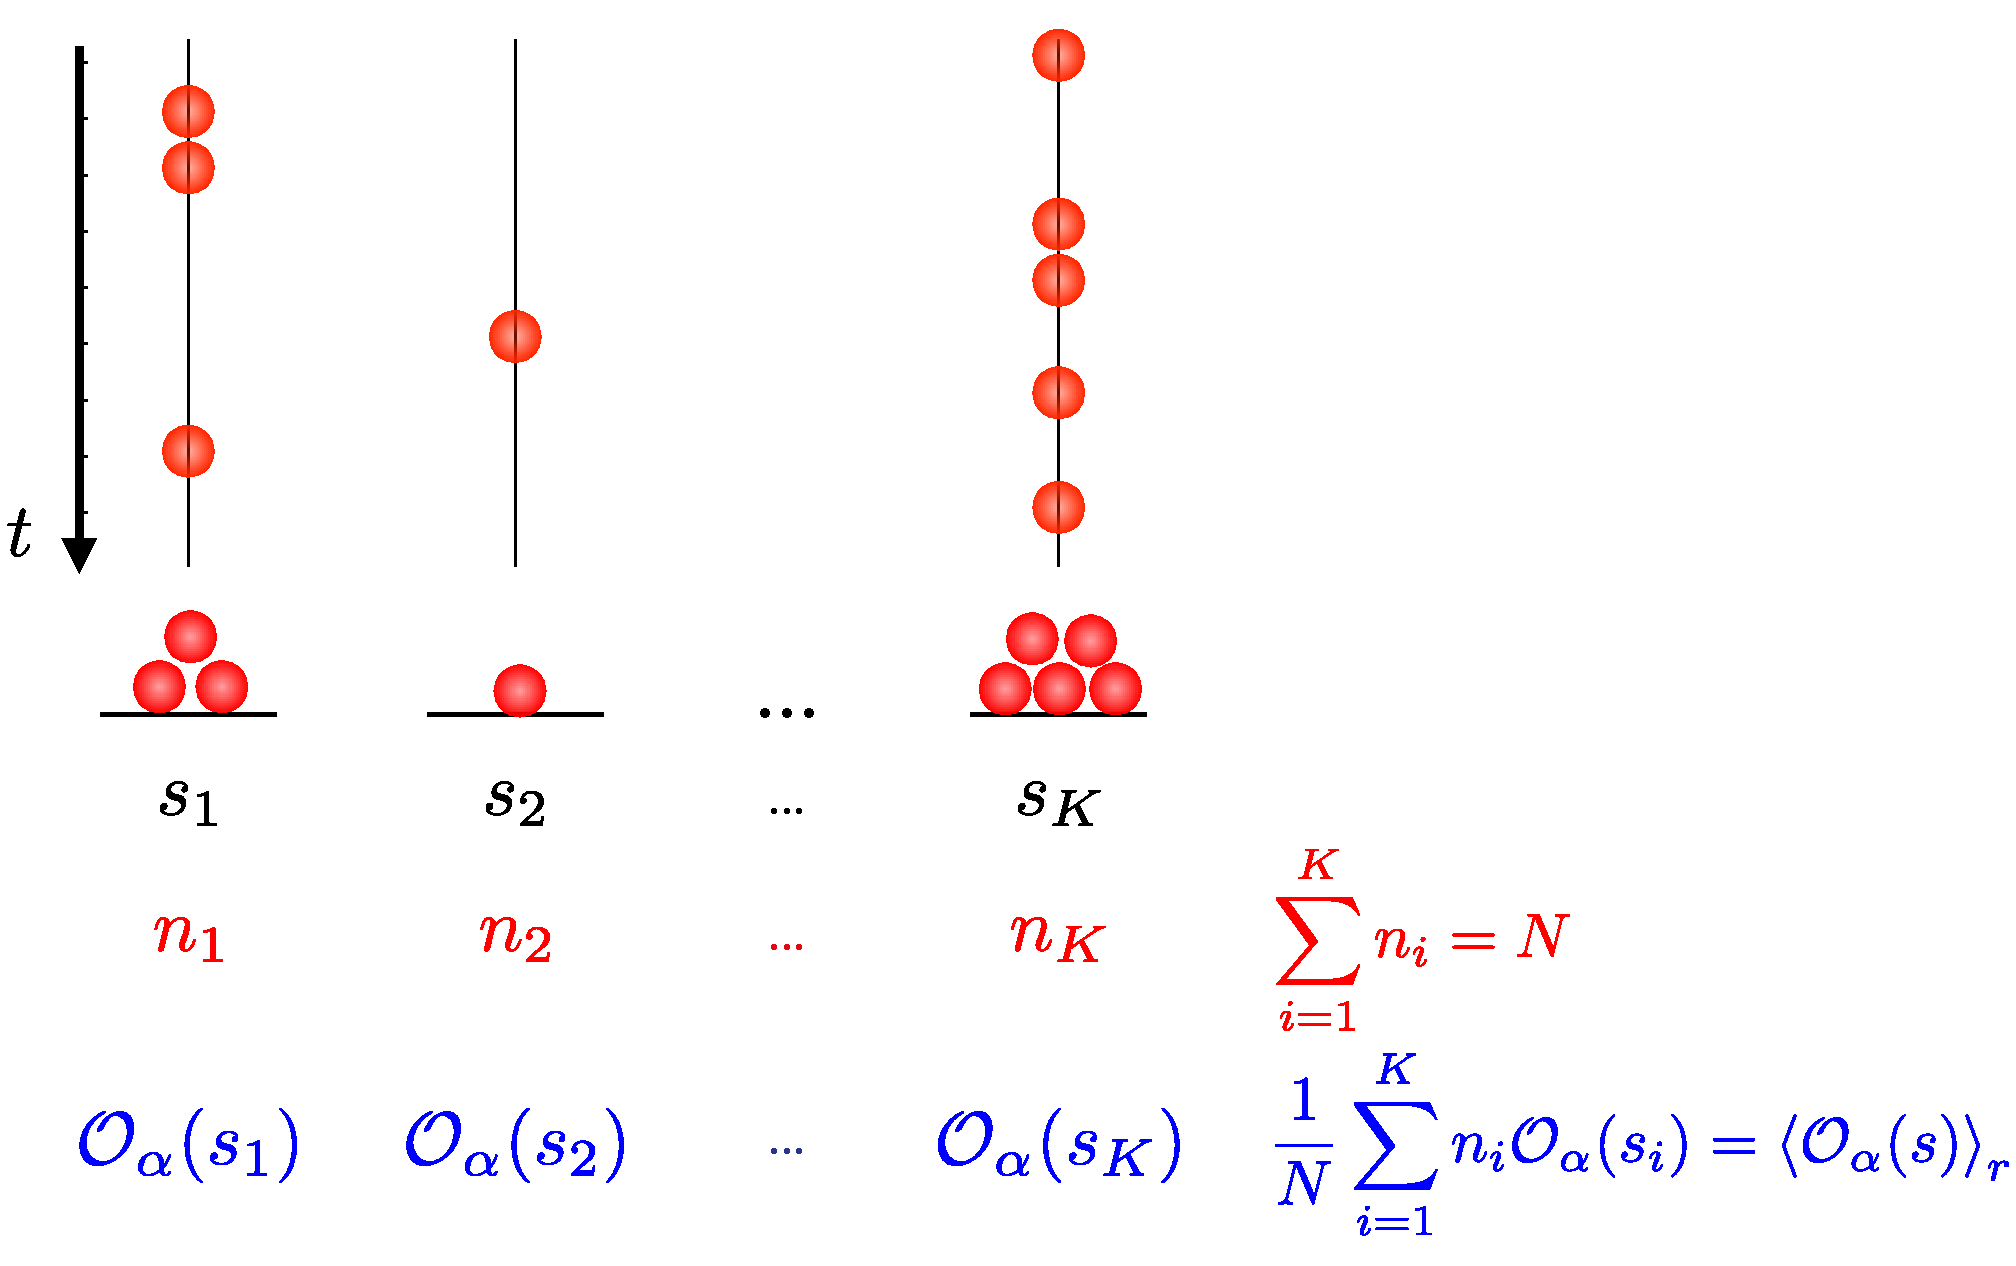
\includegraphics[width=1.0\textwidth]{figures/entropie.pdf}
\captionbf{Illustration d'un syst�me dont on veut maximiser l'entropie}{

    Le syst�me explore $K$ �tats $\{s_1,\cdots,s_K\}$ au cours du temps. Au
    bout de $N$ observations, un �tat $s_i$ a �t� observ� $n_i$ fois. � chaque
    �tat correspond un certain nombre de quantit�s $\mathcal{O}_\alpha(s_i)$
    dont seule la valeur moyenne empirique $\left\langle
    \mathcal{O}_\alpha(s)\right\rangle_r$ est connue de l'observateur (on parle
    d'\og observable \fg).

}
\label{fig:entropie}
\efig


\subsection{Pourquoi maximiser l'entropie?}
\label{sub:pourquoi_maximiser_l_entropie_}

Le concept d'entropie remonte aux pr�misses de la physique
statistique~\cite{Jaynes1978p795}. Dans l'essence, il peut �tre compris de la
mani�re suivante. Supposons qu'un syst�me comporte $K$ �tats distincts
$\{s_1,\cdots,s_K\}$. Au cours du temps, le syst�me explore les diff�rents
�tats (fig.~\ref{fig:entropie}). Au bout de $N$ observations, chaque �tat a �t�
observ� un nombre $n_i$ de fois. La question sous-jacente au calcul de
l'entropie est la suivante : sans connaissance \apriori sur le syst�me, que
puis-je dire de ces $n_i$? Prenons l'exemple de la figure \ref{fig:entropie}.
On a certaines valeurs pour les $n_i$ ($n_1=3$, $n_2=1$, etc.), et on aimerait
savoir de combien de mani�res il est possible de r�aliser un tel ensemble de
valeurs. Notons ce nombre $\mathcal{N}(n_1,\cdots,n_K)$. Il est donn� par la
formule suivante :

\begin{align}
    \begin{split}
    \mathcal{N}(n_1,\cdots,n_K) & = \binom{N}{n_1}\binom{N-n_1}{n_2}\cdots\binom{N-\sum_{i=1}^{K-1} n_i}{n_K} \\
    & = \frac{N!}{(N-n_1)!n_1!} \times \frac{(N-n_1)!}{(N-n_1-n_2)!n_2!} \times \cdots \times \frac{(N-\sum_{i=1}^{K-1}n_i)!}{0!n_K!}
    \end{split}
\end{align}

soit

\begin{equation}
   \mathcal{N}(n_1,\cdots,n_K) = \frac{N!}{n_1!n_2!\cdots n_K!} 
\end{equation}    

Il convient alors de s'int�resser au logarithme de cette quantit�. En effet, dans le cas o� les nombres d'observation sont grands $n_i \gg 1$, ceux-ci s'expriment simplement gr�ce � la formule de Stirling :

\begin{equation}
    \log(n!) \xrightarrow[n\to\infty]{} n\log(n)-n
\end{equation}

On peut alors �crire

\begin{align}
    \begin{split}
   \log\mathcal{N}(n_1,\cdots,n_K) & = N\log(N) - N - \sum_{i=1}^K \left(n_i\log(n_i) -n_i\right) \\ 
   & = \sum_{i=1}^K n_i\log(\frac{N}{n_i}) \\ 
   & = -N \sum_{i=1}^K \frac{n_i}{N}\log(\frac{n_i}{N})
   \end{split}
\end{align}

On note l'apparition des probabilit�s empiriques $f(s_i)=n_i/N$ d'observer
l'�tat $s_i$, qui tendent asymptotiquement (dans la limite \og thermodynamique \fg
$N \to \infty$) vers les \og vraies \fg probabilit�s $P(s_i)$. L'entropie est d�finie dans cette limite comme �tant �gale � $1/N\log\mathcal{N}(n_1,\cdots,n_K)$, soit

\begin{equation}
   \label{eq-entropy}
   \boxed{
   S[P] = - \sum_{\left\{ s \right\}}P(s) \log P(s)
   }
\end{equation}

o� $\{s\} = \{s_1,\cdots,s_K\}$ d�note l'ensemble des �tats accessibles. L'id�e
est alors la suivante : nous souhaitons savoir quels �tats le syst�me a le plus
probablement visit� au cours des $N$ transitions. Sans connaissance \apriori
sur le syst�me, il est plus probable que les nombres $(n_1,\cdots,n_K)$ obtenus
soient ceux qui sont r�alis�s le plus souvent, \cad ceux qui maximisent la
quantit� $\mathcal{N}(n_1,\cdots,n_K)$ et donc au final l'entropie. Par
ailleurs, les fluctuations relatives des quantit�s $n_i$ sont de l'ordre de
$1/\sqrt{n_i}$~\cite{sethna2006statistical}.  Ainsi, la solution de maximum
d'entropie domine largement les autres solutions possibles dans la limite
thermodynamique.

% subsection pourquoi_maximiser_l_entropie_ (end)

\subsection{Maximisation de l'entropie sous contraintes}
\label{sub:maximisation_de_l_entropie_sous_contraintes}

Notons $\mathcal{O}_\al(s)$ une quantit� attach�e � $s$
(fig.~\ref{fig:entropie}). En thermodynamique, une telle quantit� correspond
par exemple � l'�nergie d'un �tat. L'observateur n'a lui acc�s qu'aux valeurs
moyennes de telles quantit�s sous-jacentes. � l'�tat d'�quilibre
thermodynamique, l'�chantillonnage des �tats est r�alis� au sein de la
distribution de probabilit� de maximum d'entropie $P(s)$, et les valeurs
moyennes calcul�es avec les fr�quences empiriques $f(s)$ doivent donc �tre
compatibles avec les valeurs moyennes calcul�es avec la distribution de
probabilit� $P(s)$ :

\begin{equation}
   \label{eq:constraints}
   \sum_{\{s\}} P(s) \mathcal{O}_\al(s) = \sum_{\{s\}}f(s) \mathcal{O}_\al(s)
\end{equation}

Nous souhaiterions maintenant conna�tre la distribution $P(s)$ la moins biais�e
(i.e de maximum d'entropie) qui satisfait les contraintes de l'�q.
\ref{eq:constraints} impos�es par l'observation des donn�es (l'information que
poss�de l'observateur). Ce probl�me revient � maximiser le Lagrangien suivant :

\begin{equation}
   \mathcal{L}  =  - \sum_{\{ s \}} P(s) \log P(s) + \lambda \left(\sum_{\{ s \}}
   P(s) -1\right)  +  \sum_\al \beta_\al \sum_{\{s\}} \left( P(s) - f(s) \right) \mathcal{O}_\al(s) 
\end{equation}

o� les param�tres $\lambda$ et $\beta_\al$ sont les multiplicateurs de Lagrange
correspondant respectivement � la contrainte de normalisation de la
distribution de probabilit� et aux informations qu'a l'observateur sur
certaines valeurs moyennes du syst�me (�q. \ref{eq:constraints}).  La
maximisation de ce Lagrangien est obtenue en annulant la d�riv�e fonctionnelle
par rapport � la distribution de probabilit� $P(s)$ :

\begin{equation}
   \frac{\delta \mathcal{L}}{\delta  P(s)}   =  0  
   = - \ln P(s) - 1  + \lambda  
   +  \sum_{\al} \beta_\al \mathcal{O}_\al(s)
\end{equation}

En utilisant la normalisation des probabilit�s, il est possible de trouver
$\lambda$, et la solution se met finalement sous la forme 

\begin{equation}
    \label{eq:boltzmann}
    \boxed{
        P(s) = \frac{1}{\mathcal{Z}} e^{-\mathcal{H}(s)}
    }
\end{equation}

o� $\mathcal{H}$ est l'Hamiltonien du syst�me :

\begin{equation}
   \mathcal{H} = \sum_\al \beta_\al\mathcal{O}_\al(s)
\end{equation}

et $\mathcal{Z}$ est la fonction de partition permettant la normalisation de la
distribution $P(s)$ :

\begin{equation}
   \mathcal{Z}=\sum_{\{s\}} \exp[- \mathcal{H}(s)].
\end{equation}


\Remarque{

    \footnotesize{ Il est possible de montrer que la maximisation de
        l'entropie, partant des contraintes de l'�q. \ref{eq:constraints} sur
        les valeurs moyennes pour en arriver � une forme exponentielle de la
        distribution de probabilit�, est le contrepoint d'une maximisation de
        la vraisemblance partant d'une forme exponentielle pour en arriver aux
        m�mes contraintes sur les valeurs
        moyennes~\cite{grendar2001minimax,jaynes1982rationale}.  }

}

% subsection maximisation_de_l_entropie_sous_contraintes (end)

\subsection{Application aux sites de fixation}
\label{sub:application_aux_sites_de_fixation}

\subsubsection{Corr�lations � un point : le mod�le PWM}
\label{ssub:corr_lation_un_point_le_mod_le_pwm}

Dans le cas qui nous int�resse, un �tat $s$ correspond � une s�quence d'ADN
appartenant � l'ensemble $\left\{ s \right\}$ des sites de fixation d'un \tf.
Consid�rons maintenant l'observable quantifiant la pr�sence du nucl�otide $a$
� la position $i$ d'un site :

\begin{equation}
    \mathcal{O}_{i,a}(s) = \delta(s_i,a)
\end{equation}


o� $\delta$ est la fonction de Kronecker qui vaut $1$ lorsque le nucl�otide
� la position $i$ du site $s_i$ vaut $a$ et $0$ sinon. De cette d�finition il suit que la valeur moyenne sur les fr�quences empiriques


\begin{equation}
    \label{eq:onepoint}
    \sum_{\{s\}} f(s) \mathcal{O}_{i,a}(s) = f_{i,a}
\end{equation}

se r�duit � la fr�quence du nucl�otide $a$ � la position $i$. Notons $h_i(a)$
le multiplicateur de Lagrange correspondant et $\mathcal{A} = \{A,C,G,T\}$. On trouve alors

\begin{align}
    \begin{split}
    \mathcal{H}(s) & = \sum_{i=1}^L \sum_{a \in \mathcal{A}} h_i(a) \delta(s_i,a)\\
     & = \sum_{i=1}^L h_{i}(s_i)
    \end{split}
\end{align}

Les diff�rentes positions �tant ind�pendantes, la fonction de partition
$\mathcal{Z}$ peut par ailleurs se scinder en diff�rentes fonctions de partition par
position : $\mathcal{Z}=\prod_{i=1}^L\mathcal{Z}_i$. On obtient au final

\begin{equation}
    P(s) = \frac{1}{\mathcal{Z}} e^{-\sum\limits_{i=1}^L h_i(s_i)} = \prod_{i=1}^L \frac{e^{-h_i(s_i)}}{\mathcal{Z}_i}
\end{equation}

On retrouve le mod�le PWM introduit dans l'�q.~\ref{eq:boltzmann}.



% subsubsection corr_lation_un_point_le_mod_le_pwm (end)

\subsubsection{Corr�lations � deux points : le mod�le de Potts}
\label{ssub:corr_lations_deux_points_le_mod_le_de_potts}


Il est maintenant relativement direct de complexifier le mod�le en ajoutant
l'observation des couples d'interaction au sein des sites de fixation :

\begin{equation}
    \mathcal{O}_{i,a,j,b}(s) = \delta(s_i,a)\delta(s_j,b)
\end{equation}

La corr�lation � deux points entre le nucl�otide $a$ en position $i$ et $b$ en
position $j$ s'�crit donc 

\begin{equation}
    \label{eq:twopoints}
    \sum_{\{s\}} f(s) \mathcal{O}_{i,a,j,b}(s) = f_{i,a,j,b}
\end{equation}

o� $f_{i,a,j,b}$ est la fr�quence empirique d'observation de la paire de
nucl�otide $(a,b)$ aux positions $(i,j)$. Notons $J_{i,j}(a,b)$ le
multiplicateur de Lagrange correspondant. L'Hamiltonien sous les contraintes
impos�es par les �quations \ref{eq:onepoint} et \ref{eq:twopoints} s'�crit :


\begin{align}
    \begin{split}
    \mathcal{H}(s) & = \sum_{i=1}^L \sum_{a \in \mathcal{A}} h_i(a) \delta(s_i,a) + \sum_{i=1}^{L-1} \sum_{j>i} \sum_{a \in \mathcal{A}} \sum_{b \in \mathcal{A}} J_{i,j}(a,b) \delta(s_i,a)\delta(s_j,b)\\
    & = \sum_{i=1}^L h_{i}(s_i) + \sum_{i=1}^{L-1}\sum_{j>i} J_{i,j}(s_i,s_j)
\end{split}
\end{align}

Le mod�le de maximum d'entropie est finalement

\begin{equation}
    \label{eq:potts}
    \boxed{
    P(s) = \frac{1}{\mathcal{Z}} e^{-\sum\limits_{i=1}^L h_i(s_i)-\sum\limits_{i=1}^{L-1} \sum\limits_{j>i} J_{i,j}(s_i,s_j)} 
}
\end{equation}

On reconna�t le mod�le de Potts inhomog�ne de champs magn�tiques locaux $h_i$
et de termes d'interaction $J_{i,j}$ couramment utilis� dans la description des
verres de spins~\cite{baxter2007exactly}.


% subsubsection corr_lations_deux_points_le_mod_le_de_potts (end)

% subsection application_aux_sites_de_fixation (end)


\section{Article} 
\label{sec:article_maxent}

L'article qui suit d�crit l'analyse de donn�es de fixation \invivo � grande �chelle
pour plusieurs TFs drosophiles et mammif�res. Diff�rents mod�les sont compar�s,
incluant ou non des d�pendances : un mod�le PWM, un mod�le de m�lange de PWMs,
et un mod�le de Potts.


\includepdf[pages=-]{articles/maxent-arxiv}

% section article (end)


\section{Analyse thermodynamique des mod�les} 
\label{sec:analyse_thermodynamique_des_mod_les_ind_pendant_et_avec_couplages}
\subsection{Chaleur sp�cifique}
\label{sub:chaleur_sp_cifique}


En plus des r�sultats pr�sent�s dans l'article, nous nous sommes int�ress�s
� une quantit� classique de la thermodynamique : la chaleur sp�cifique ou
capacit� calorifique. Consid�rons un mod�le d�crit par la statistique de
Boltzmann � la temp�rature inverse $\beta=1/T$ (on omet la constante de
Boltzmann $k$ en l'int�grant � l'�nergie):

\begin{equation}
    \label{eq:boltzmann_with_beta}
    P(s) = \frac{1}{\mathcal{Z}} e^{-\beta E(s)}
\end{equation}

Le cas de l'�quation \ref{eq:potts} correspond au cas particulier $\beta=1$.
Nous voulons voir comment l'amplification ou la diminution globale de l'�cart
entre les �nergies affecte la possibilit� du syst�me d'explorer les diff�rents
�tats possibles. � temp�rature nulle ($T\to0 $ ou $\beta \to \infty$), le
syst�me reste dans le niveau fondamental de minimum d'�nergie et de probabilit�
$1$, alors qu'� des temp�ratures non nulles le syst�me � l'�nergie $E_0$
transite vers un �tat d'�nergie sup�rieure $E_1$ avec une probabilit� $\propto
\exp\left(-\beta (E_1-E_0)\right)$. Lorsqu'un paysage �nerg�tique est compos�
de plusieurs puits d'�nergie s�par�s par des barri�res �nerg�tiques
importantes, on s'attend � avoir une (ou plusieurs) temp�ratures critiques
� partir desquelles de fortes diff�rences d'�nergie deviennent franchissables.
L'�nergie moyenne peut alors �tre significativement affect�e, sautant
soudainement � une nouvelle valeur du fait du poids des nouveaux �tats
explor�s. 

La chaleur sp�cifique permet de caract�riser ces sauts soudains d'�nergie
moyenne lors de la variation de la temp�rature, caract�ristiques des
transitions de phase. Elle mesure simplement la variation de l'�nergie moyenne
lors d'une variation de temp�rature :

\begin{equation}
    C(T) = \frac{d\langle E \rangle}{dT}
\end{equation}

o� 

\begin{equation}
    \langle E \rangle = \sum_{\{s\}} E(s) \frac{e^{-\beta E(s)}}{\mathcal{Z}}
\end{equation}

Cette chaleur sp�cifique peut par ailleurs s'�crire sous une forme plus pratique : 

\begin{align}
    \label{eq:fluctuation-dissipation}
    \begin{split}
        \frac{d\langle E \rangle}{dT} & = - \beta^2 \frac{d\langle E \rangle}{d\beta} \\
        & = - \beta^2 \left[\sum_{\{s\}} E(s) \left( -E(s) e^{-\beta E(s)} \right)\frac{1}{\mathcal{Z}} + \sum_{\{s\}} E(s) e^{-\beta(E(s))} \left(-\frac{d\mathcal{Z}}{d\beta} \frac{1}{\mathcal{Z}^2}\right)\right] \\
    & = \beta^2 \left[ \langle {E}^2 \rangle - {\langle E \rangle}^2 \right]
    \end{split}
\end{align}

Ainsi, la chaleur sp�cifique $C(T)$ est directement accessible en regardant les
corr�lations de l'�nergie sur l'ensemble des �tats du syst�me, ce qui peut se
calculer simplement � partir des mod�les de fixation.  Nous avons calcul� la
variation de $C(T)$ en fonction de la temp�rature pour les mod�les ind�pendant
et avec d�pendances obtenus en \ref{sec:article_maxent} pour les diff�rents TFs
�tudi�s. Une temp�rature fictive est introduite dans les mod�les en multipliant
les �nergies par $\beta$, afin de se placer dans le cadre de l'�quation
\ref{eq:boltzmann_with_beta}. Les r�sultats sont montr�s en
figure~\ref{fig:maxent/specific_heat} (mod�le ind�pendant en bleu, mod�le de
Potts en rouge). On observe pour la plupart des facteurs l'existence de deux
pics de chaleur sp�cifique pour des temp�ratures de l'ordre de $T\sim10^{-1}$
et $T\sim 5$ (par exemple, $T=0.4$ et $T=2.8$ dans le cas du mod�le ind�pendant
de Twist). Il y a de l�g�res variations entre les deux mod�les : notamment, le
premier pic semble renforc� par le mod�le de Potts dans plusieurs cas (par
exemple, E$2$f$4$, NRSF, TCF$3$ ou Twist). N�anmoins, le nombre de pics (ou de
transitions de phases) reste le m�me.

\bfig
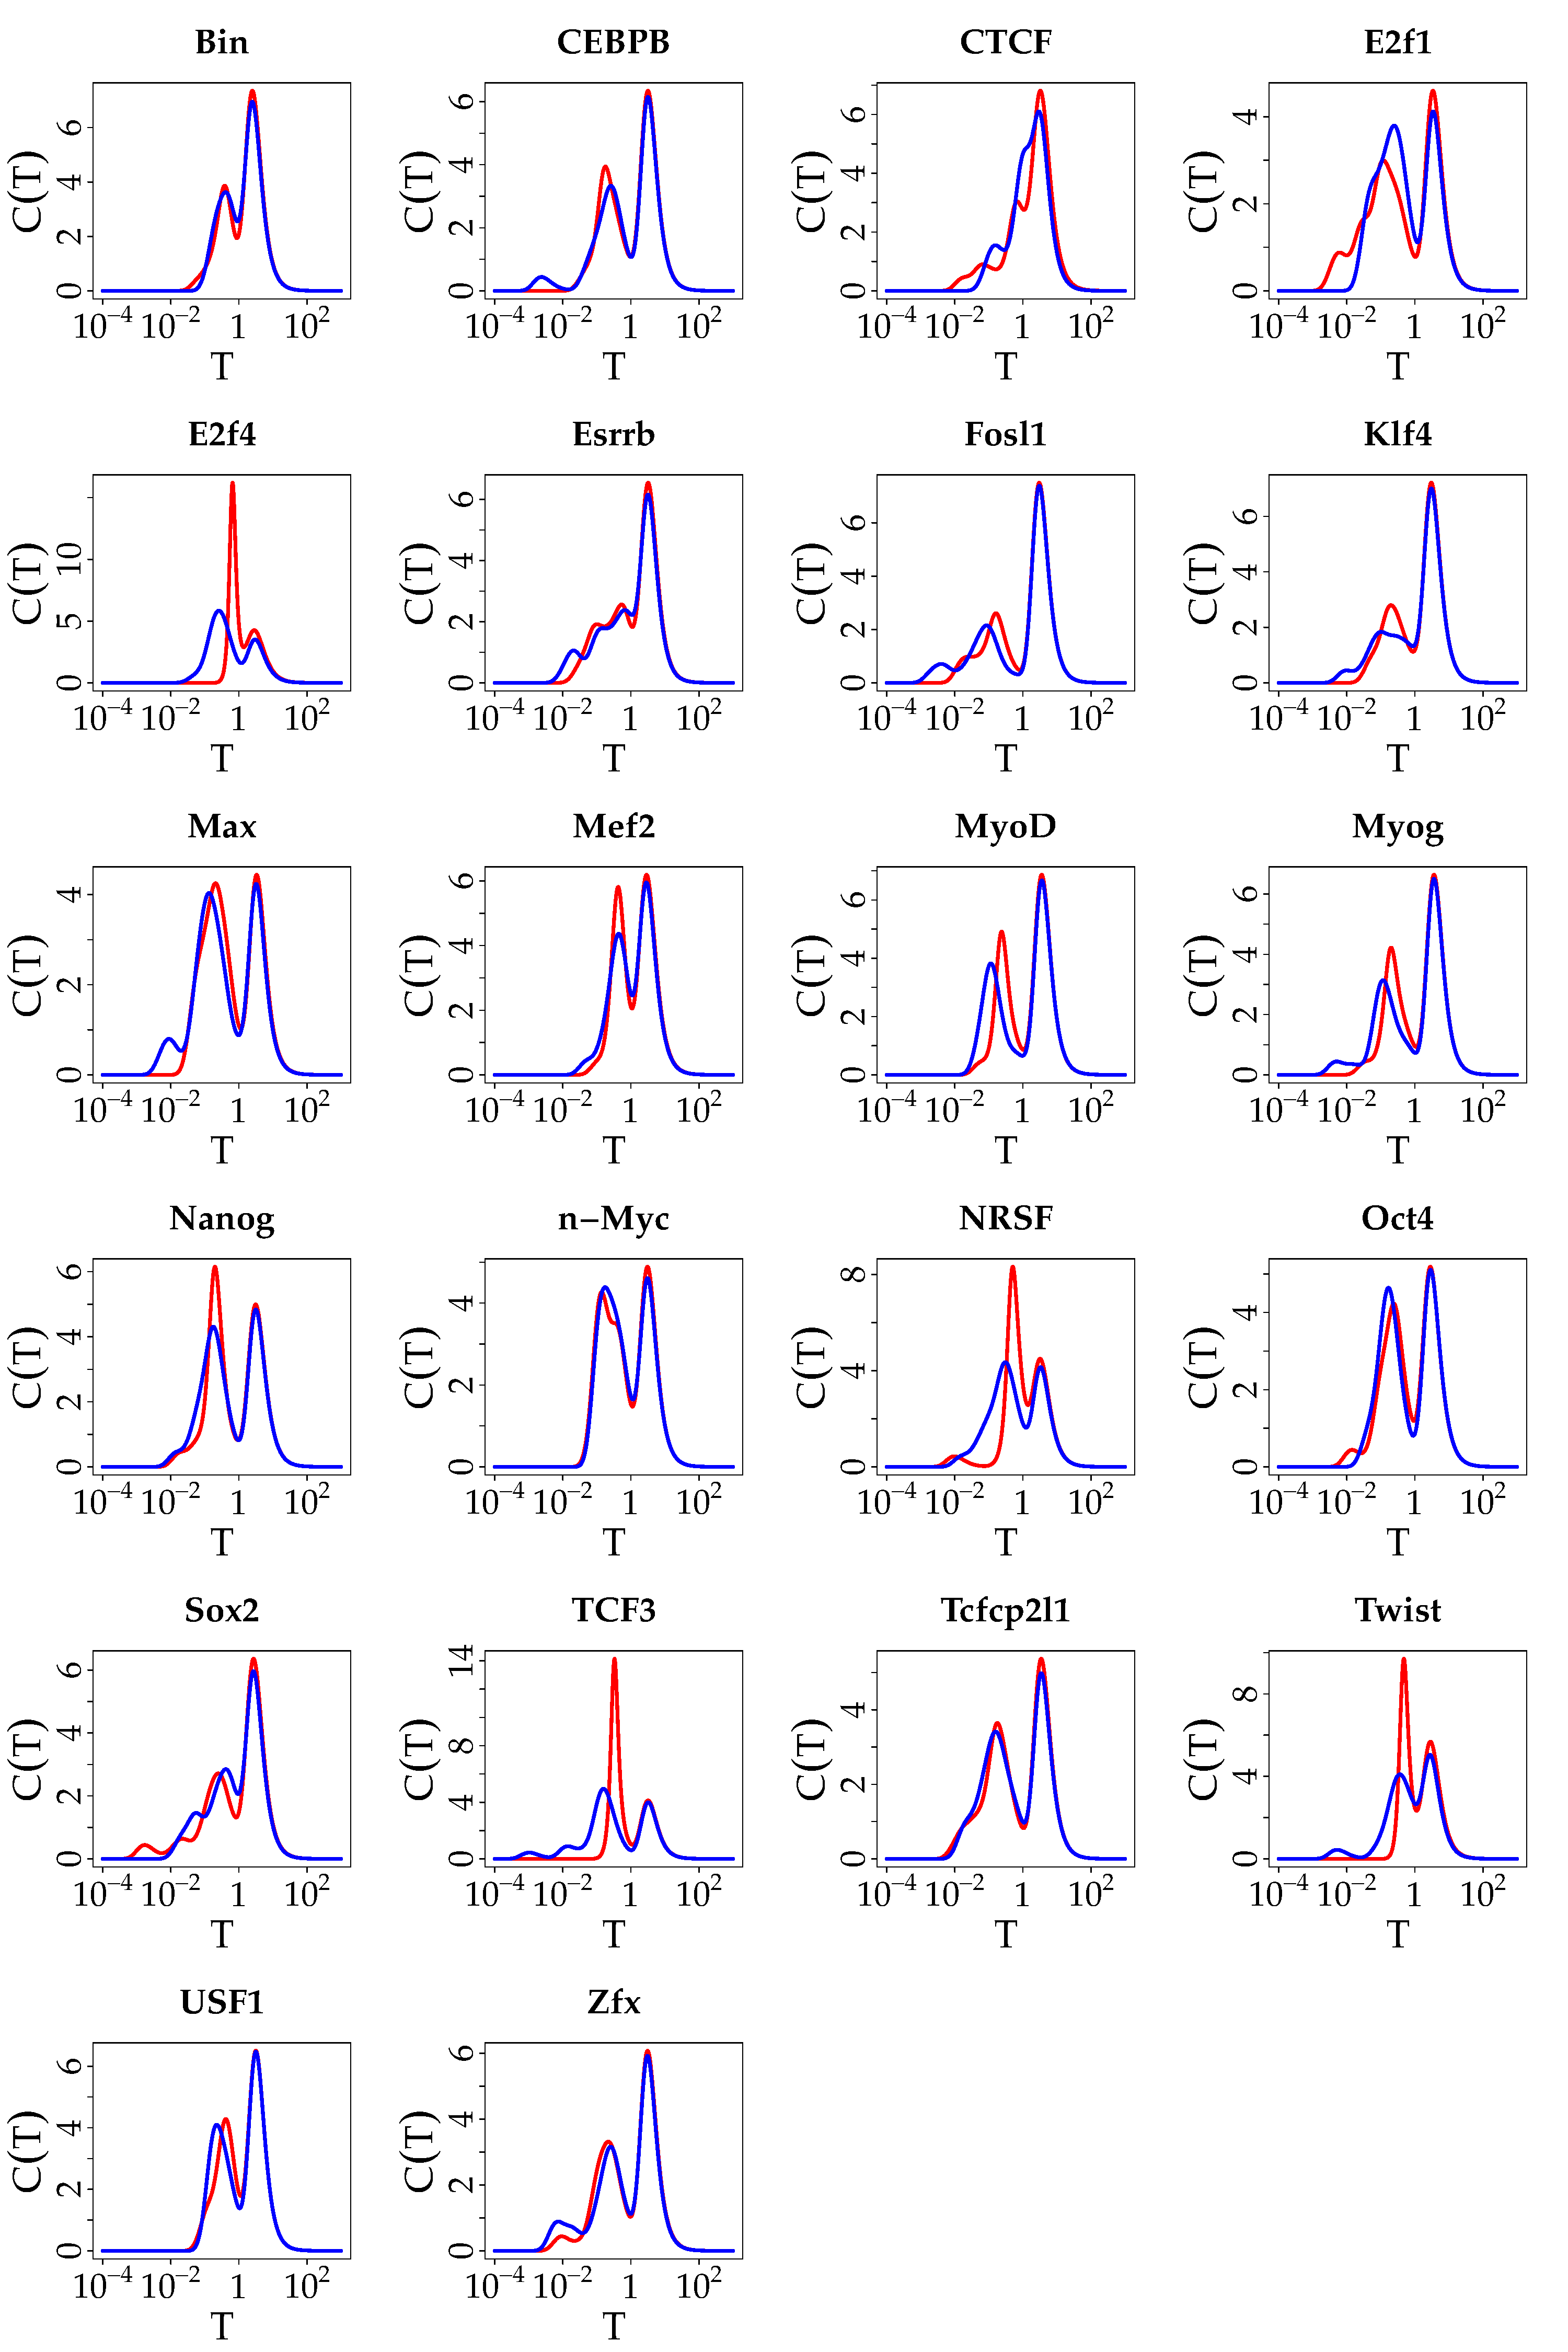
\includegraphics[width=0.8\textwidth]{figures/maxent/specific_heat.pdf}
\captionbf{Chaleur sp�cifique pour diff�rents TFs}{

    La chaleur sp�cifique (l'�quivalent de la capacit� calorifique en
    thermodynamique) $C(T)=d\langle E\rangle/dT$ est trac�e en fonction de la
    temp�rature $kT$ (�chelle logarithmique) pour les diff�rents TFs
    consid�r�s. Le mod�le ind�pendant (bleu) et le mod�le de Potts avec
    interactions (rouge) sont comparables dans la plupart des cas.

}
\label{fig:maxent/specific_heat}
\efig

% subsection chaleur_sp_cifique (end)

\subsection{Lien avec les valeurs des champs et des couplages}
\label{sub:lien_avec_les_valeurs_des_champs_et_des_couplages}

Afin de comprendre l'existence des pics de chaleur sp�cifique et les �nergies
(temp�ratures) associ�es, il faut revenir aux mod�les d'�nergie. Lorsque l'on
regarde l'histogramme des valeurs absolues de $h_i$ obtenues dans les mod�les
ind�pendant des diff�rents TFs �tudi�s, on trouve plusieurs valeurs typiques
autour de $10^{-4}$, $1$ et $10$ (fig.~\ref{fig:histogrammes_champs}A).
Celles-ci peuvent s'expliquer de la mani�re suivante. Dans le mod�le
ind�pendant, les champs sont simplement le logarithme naturel de la probabilit�
d'observer un nucl�otide $a$ � une position $i$ donn�e $h_i(a) = -\log P_i(a)$
(la jauge est choisie telle que $\mathcal{Z_i}=1$). En valeur absolue, les
champs $h_i$ proches de $0$ ($h_i\sim10^{-4}-10^{-3}$) correspondent aux
nucl�otides tr�s conserv�s (toujours observ�s), les valeurs autour de $1$
correspondent � des nucl�otides d�g�n�r�s (i.e �galement observ�s
: $|\log(1/4)| \sim 1.4$) et les valeurs autour de $10$ correspondent aux
nucl�otides qui ne sont jamais observ�s, au pseudocount pr�s (pour un
pseudocount de $1$ et $10^4$ s�quences, $|\log(10^{-4})| \sim 9.2$).  On peut
maintenant mieux comprendre les pics de chaleur sp�cifique. � temp�rature
nulle, seuls les sites consensus sont accessibles. Lorsque la temp�rature se
rapproche de $1$, les nucl�otides d�g�n�r�s d'�nergie $h_i\sim1$ deviennent
accessibles, augmentant significativement la valeur de l'�nergie moyenne
(premier pic). Puis, lorsque la temp�rature se rapproche de $10$, les
nucl�otides non observ�s d'�nergie $h_i\sim10$ deviennent � leur tour
accessibles, augmentant � nouveau l'�nergie moyenne (deuxi�me pic).

Dans le cas du mod�le de Potts (fig.~\ref{fig:histogrammes_champs}B), les
champs $h_i$ prennent des valeurs proches de celles obtenues avec le mod�le
ind�pendant. Par ailleurs, les interactions $J_{i,j}$ sont r�parties autour
d'un mode centr� autour de $J_{i,j} \sim 0.5$, ce qui correspond l'�chelle
d'�nergie du premier pic. Ainsi, le renforcement du premier pic de chaleur
sp�cifique par rapport au cas ind�pendant observ� pour plusieurs TFs de la
figure \ref{fig:maxent/specific_heat} peut s'expliquer par l'effet des termes
d'interaction $J_{i,j}$.


\bfig
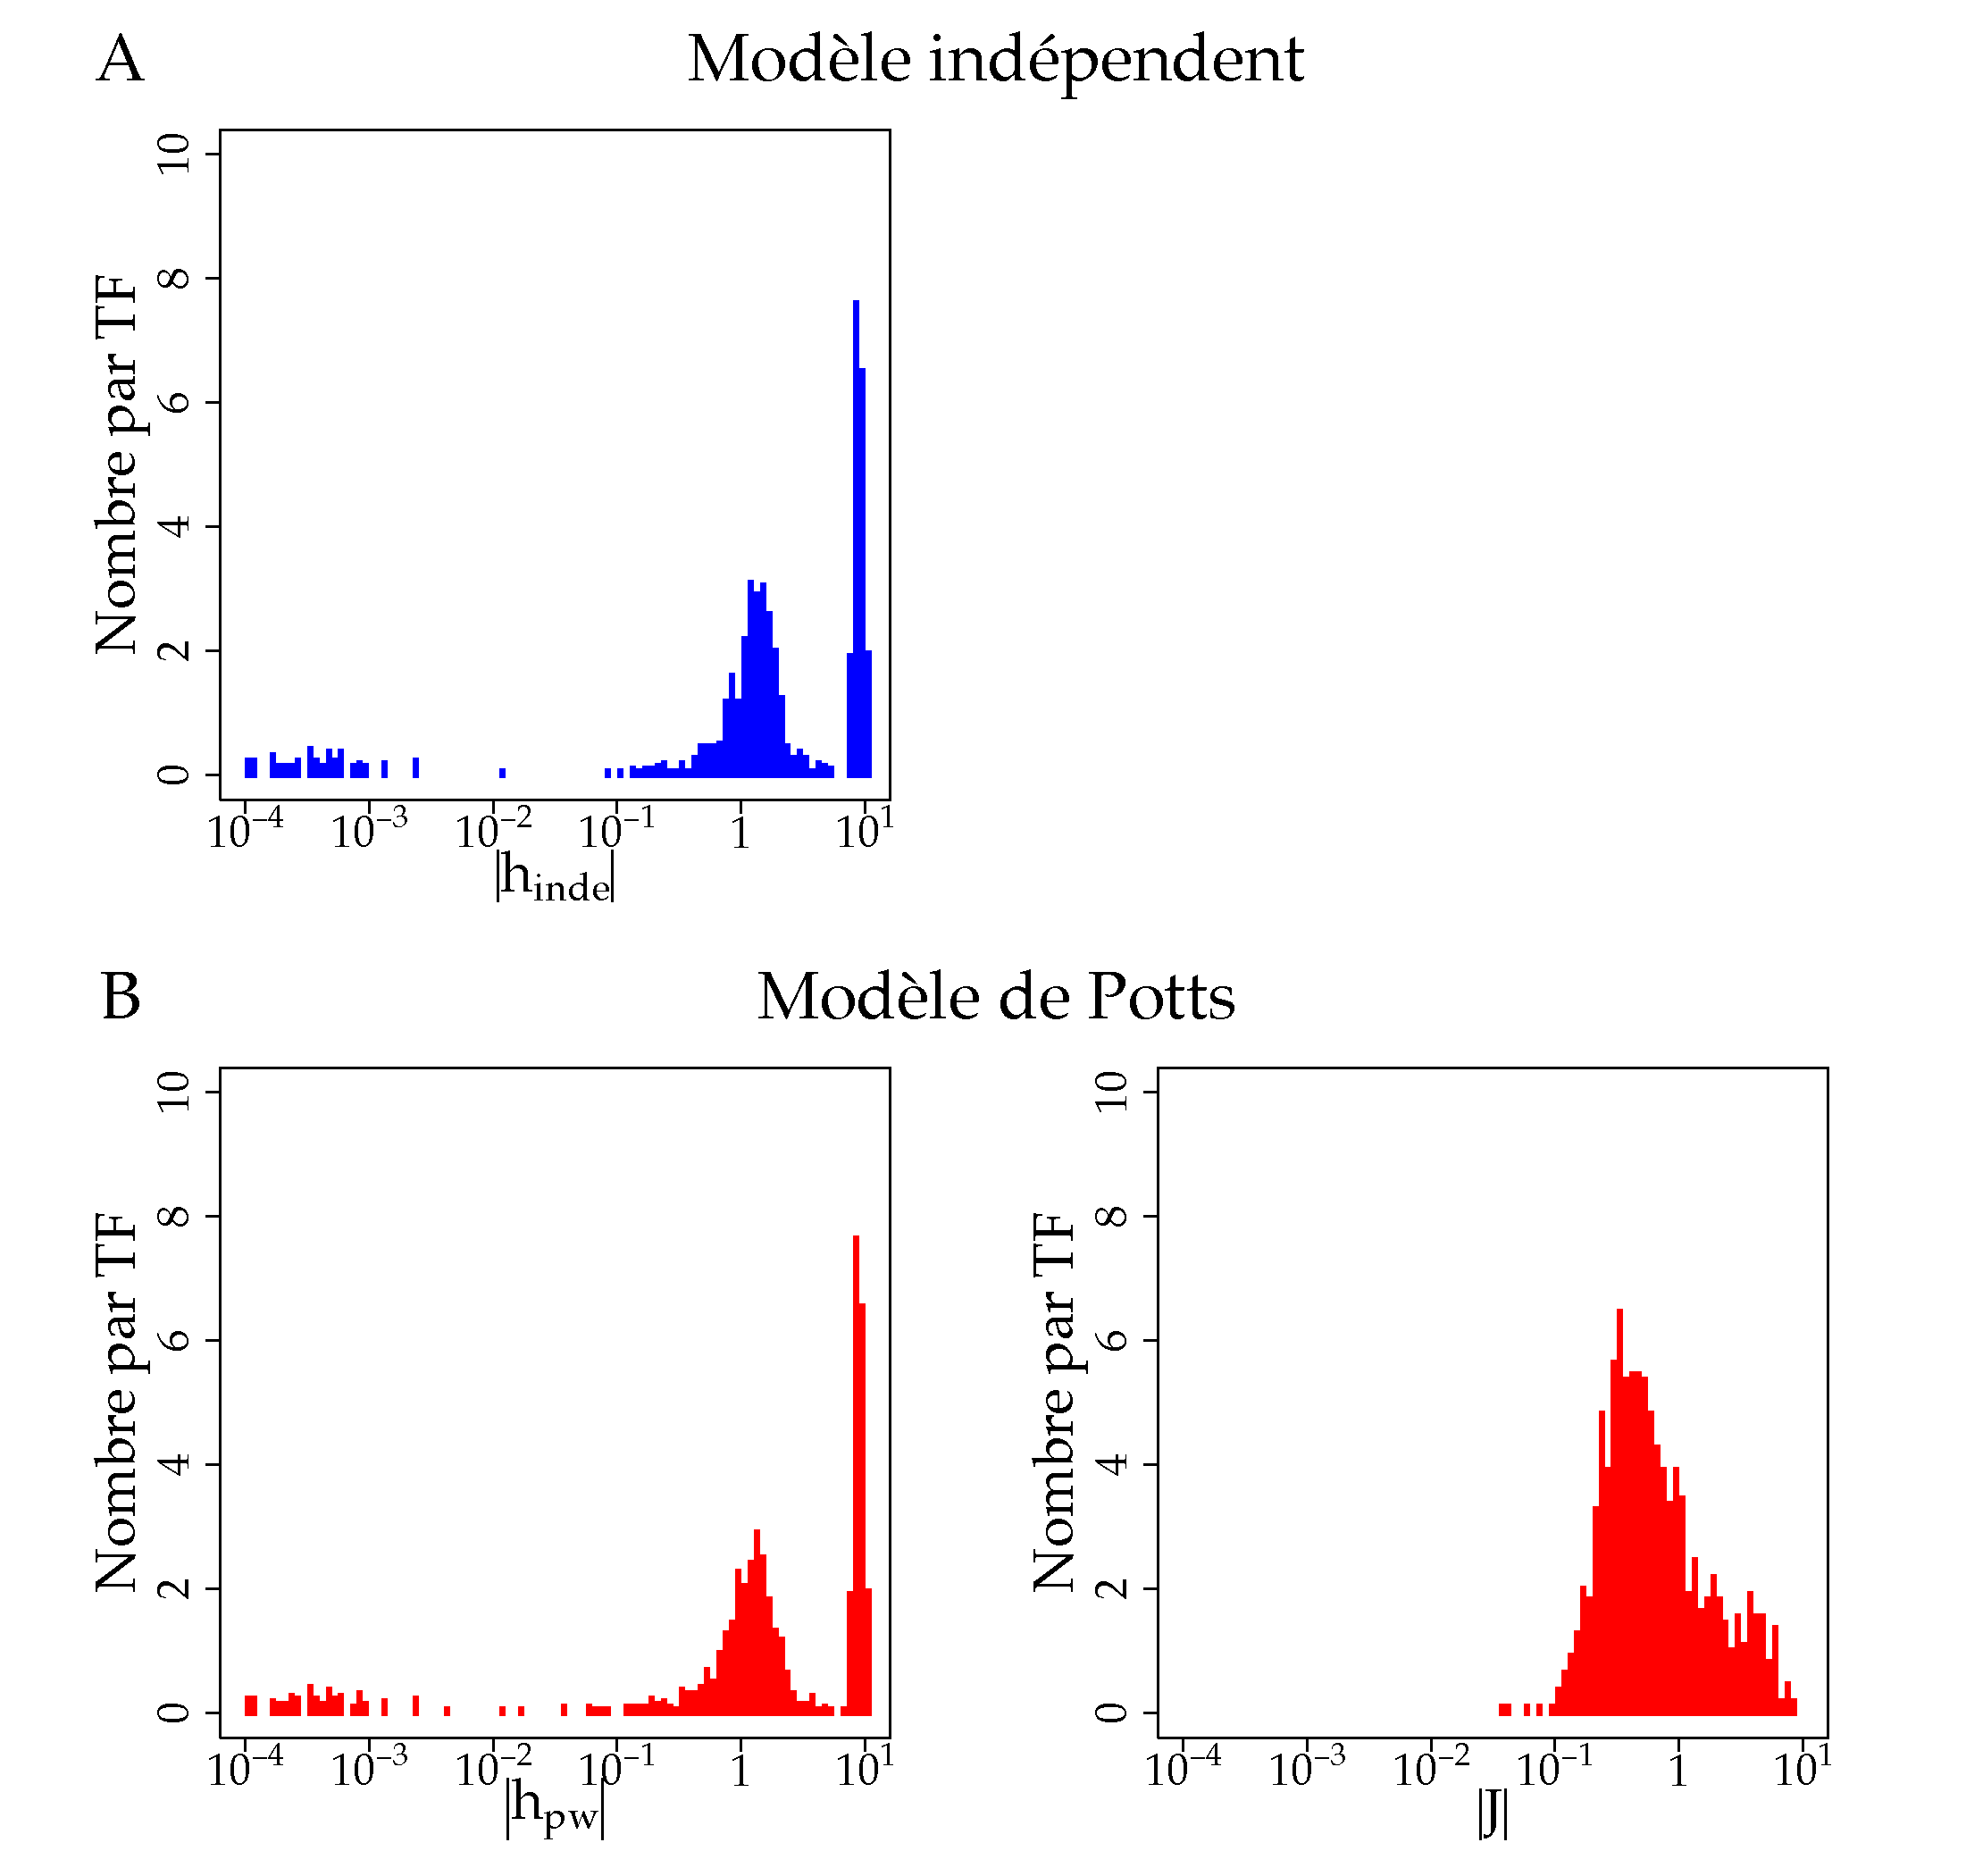
\includegraphics[width=1.\textwidth]{figures/maxent/histogrammes_champs.pdf}
\captionbf{Histogrammes des valeurs des champs $h$ et couplages $J$}{

    Histogrammes r�alis�s � partir des valeurs obtenues pour l'ensemble des
    TFs. Les champs et les couplages sont montr�s en valeur absolue sur une
    �chelle logarithmique d'espacement $0.05$, et les valeurs nulles ne sont
    pas repr�sent�es. (A) Champs $h_{inde}$ dans le mod�le ind�pendant. (B)
    Champs $h_{pw}$ et couplages $J$ dans le mod�le de Potts.

}
\label{fig:histogrammes_champs}
\efig


% subsection lien_avec_les_valeurs_des_champs_et_des_couplages (end)

% section analyse_thermodynamique_des_mod_les_ind_pendant_et_avec_couplages (end)
\section{Conclusion et perspectives du chapitre \thechapter}


Nous avons analys� les d�pendances au sein des sites de fixation li�s \invivo
pour diff�rents \tfs Drosophiles et mammif�res. Nous avons compar� les
performances d'un mod�le PWM, d'un mod�le de m�lange de PWMs, et d'un mod�le de
Potts, en utilisant un crit�re bay�sien (BIC) p�nalisant les mod�les � grand
nombre de param�tres. Nous avons exhib� l'existence de corr�lations faibles
dont la prise en compte permet de significativement am�liorer la description
des donn�es, le mod�le de Potts �tant significativement sup�rieur aux deux
autres mod�les dans la plupart des cas ($22/28$). Les interactions ont �t�
�tudi�es syst�matiquement, montrant notamment une pr�pond�rance des
interactions entre plus proches voisins. Nous avons �tabli une correspondance
entre les PWMs du mod�le de m�lange et les PWMs d�crivant les �tats
m�tastables du paysage �nerg�tique g�n�r� par le mod�le de Potts. Enfin, nous
avons montr� que les corr�lations pouvaient �tre group�es en patterns de
Hopfield ou \og m�moires \fg, et qu'un petit nombre �tait suffisant
� reconstruire le paysage d'interactions.  \\

Une perspective int�ressante de ce travail serait de conduire la m�me analyse
sur des donn�es grande �chelle obtenues \invitro par la m�thode
HT-SELEX~\cite{Jolma2013p3971}. Notamment, certains des facteurs que nous avons
�tudi�s \invivo sont repr�sent�s dans ces donn�es, et il serait int�ressant de
voir les diff�rences entre les mod�les obtenus. Notamment, retrouve-t-on les
m�mes corr�lations? Peut-on exhiber des sp�cificit�s de la fixation \invivo, o�
l'on s'attend � avoir des effets provenant de diverses sources (fixation de
nucl�osomes, superposition de sites de fixations, \ldots)? Ces questions feront
certainement l'objet d'un prochain travail.



\newpage

%%%%%%%%%%%%%%%%%%%%%%%%%%%%%%%%%%%%%%%%%%%%%%%%%%%%%%%%%%%%%%%%%%%%%%%%%%%%%%%%%%%%%%%%%%
\chapter{\ChImogene} 
\label{ch:imogene}
%\adjustmtc
\minitoc
\newpage
\section*{Introduction du chapitre \thechapter}

Dans le chapitre \ref{ch:maxent}, nous avons vu comment d�crire l'interaction
TF-ADN lorsque des sites de fixation sont connus. Dans ce chapitre, nous
adoptons une d�marche plus g�n�rale. Nous connaissons l'activit� de r�gulation
d'un certain nombre de CRMs, et nous souhaitons savoir quels TFs s'y fixent
(recherche de motifs), et si le g�nome contient d'autres CRMs avec la m�me
activit� (recherche de modules). Un algorithme permettant pr�cis�ment de
r�aliser ces �tapes a �t� d�velopp� pr�c�demment par Herv� Rouault et appliqu�
au cas de la diff�renciation des organes sensoriels de la
Drosophile~\cite{Rouault2010p327}. Cet algorithme se distingue des pr�c�dents
par le fait qu'il n'utilise pas de motifs connus en entr�e mais les g�n�re
purement \denovo, et par son utilisation syst�matique de l'information
provenant de la conservation chez d'autres esp�ces gr�ce � des mod�les
d'�volution, le rendant notamment adapt� au cas o� les CRMs connus sont en
petit nombre. Nous pr�sentons ici Imogene, l'extension de cet algorithme au cas
des mammif�res, ainsi que son utilisation comme outil de classification de CRMs
associ�s � diff�rentes r�gulations.

Avant de rentrer dans le d�tail d'Imogene, nous pr�sentons les m�thodes
existantes de recherche de motifs dans des CRMs. Le probl�me g�n�ral est le
suivant : �tant donn�es des CRMs conduisant � une m�me r�gulation (l'ensemble
d'apprentissage), peut-on construire des mod�les de sites de fixation qui \og
expliquent \fg cette co-r�gulation, \cad qui pr�disent l'existence de sites sur
les CRMs mais pas sur des s�quences ne participant pas � la co-r�gulation?



\section{Quelques approches existantes pour la recherche de motifs et de modules de r�gulation} 
\label{sec:approches_existantes}

Nous avons d�j� introduit diff�rentes m�thodes de pr�diction de motifs et
modules en introduction (section \ref{sec:prediction_crms}). Ici nous d�crivons
plus en avant certaines de ces m�thodes que nous jugeons utiles � la mise en
perspective d'Imogene, soit par leur approche de g�n�ration \denovo de motifs,
soit par leur utilisation de la conservation chez d'autres esp�ces et de
mod�les d'�volution pour la prendre en compte, soit par le fait qu'elles
d�veloppent des statistiques appropri�es � l'�tude de petits �chantillons de
CRMs. Pour une revue plus exhaustive, le lecteur int�ress� pourra se r�f�rer
� \citet{Wasserman2004p624} et \citet{Aerts2012p3868}.

\subsection{MEME : une approche \denovo par Esp�rance-Maximisation}
\label{sub:meme_une_approche_de_type_esp_rance_maximisation}

L'une des premi�res approches pour la pr�diction \denovo de motifs � partir de
s�quences a �t� celle de MEME~\cite{Bailey1994fk}, un algorithme bas� sur la
m�thode d'Esp�rance-Maximisation ou EM (\textit{Expectation Maximization})
utilis�e pr�c�demment dans ce cadre par \citet{Lawrence1990uq}. Cet algorithme
utilise une approche g�n�rative pour d�crire les processus probabilistes qui
ont permis la g�n�ration des s�quences CRMs, ce qui permet d'�crire la
probabilit� qu'une s�quence soit g�n�r�e par un motif, et inversement de
trouver le meilleur motif d�crivant des s�quences donn�es. L'approche est
illustr�e en figure~\ref{fig:d_haeseleer-MEME}. 

\bfig
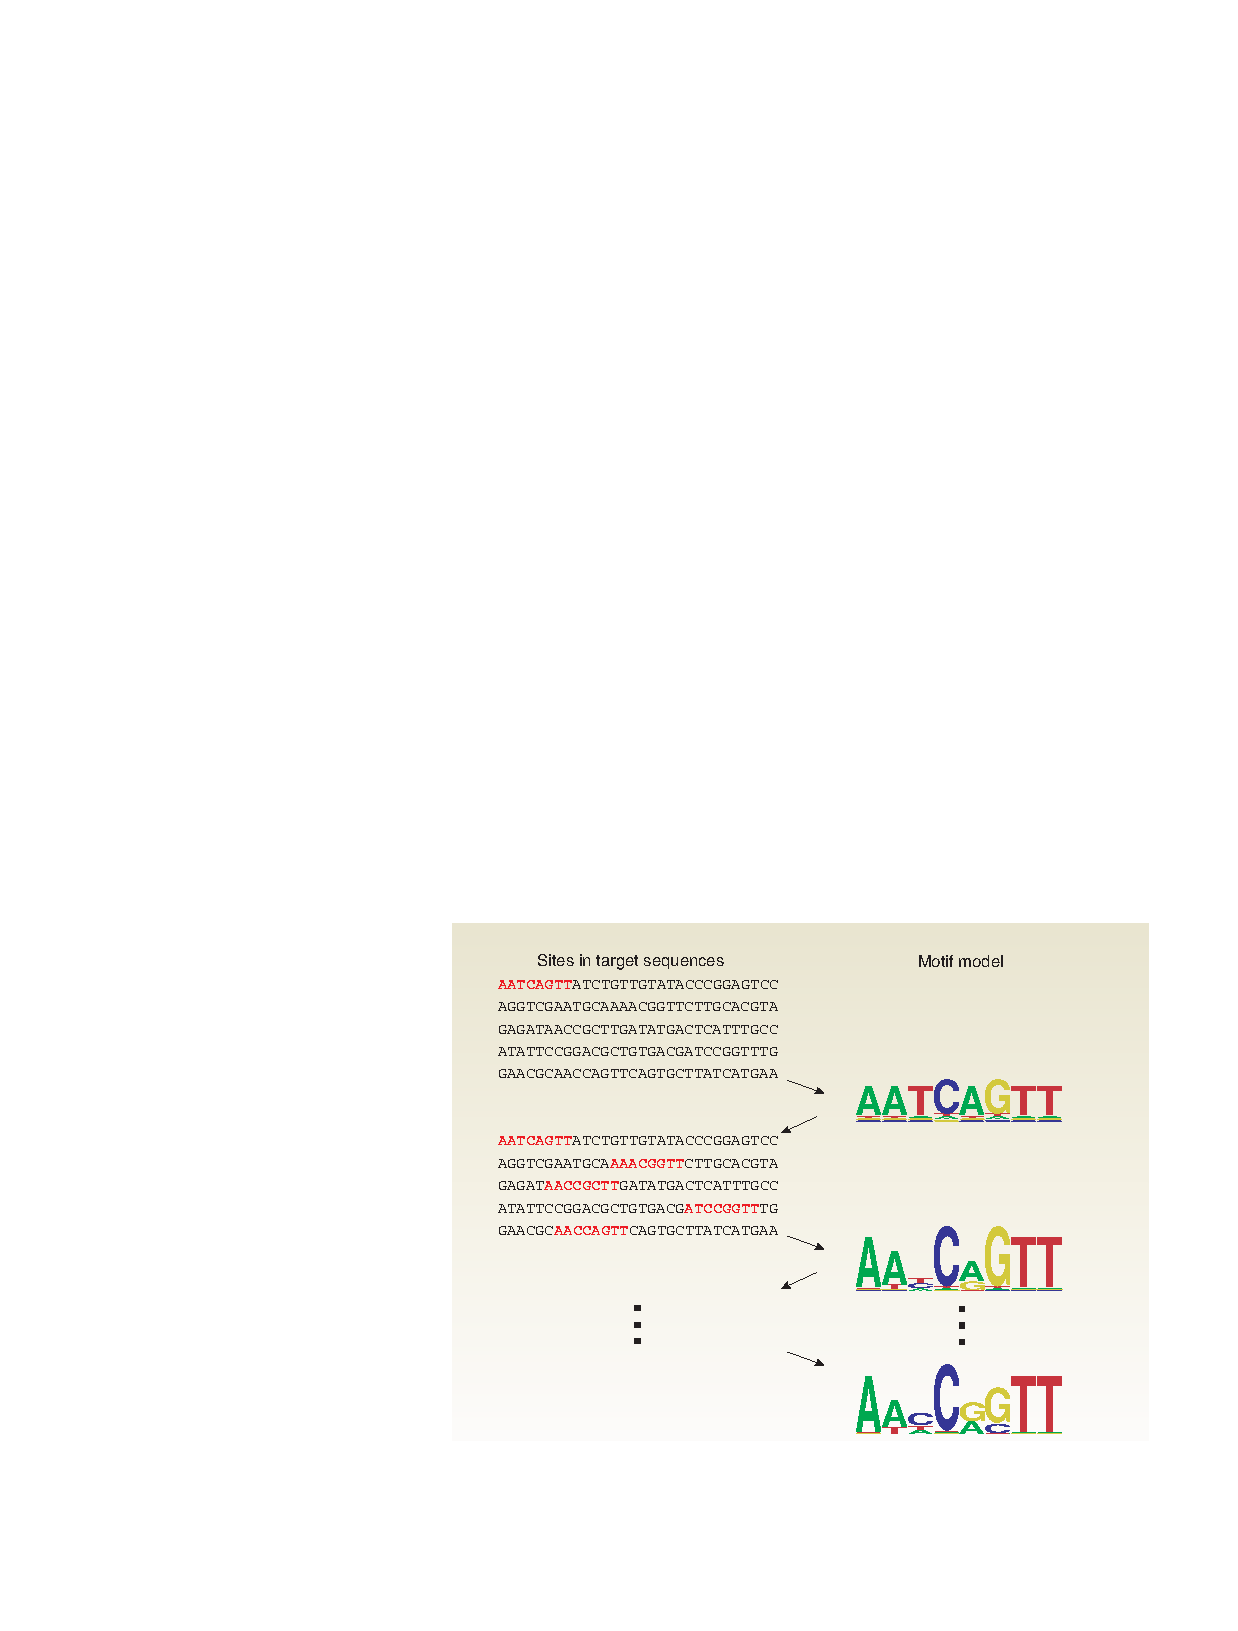
\includegraphics[width=0.8\textwidth]{figures/d_haeseleer-MEME.pdf}
\captionbf{Illustration de l'approche Esp�rance-Maximisation}{

Figure tir�e de \citet{Dhaeseleer2006kx} d�crivant l'approche EM. Un premier
mod�le de motif est construit � partir d'un site initial. Ce mod�le permet de
pond�rer l'ensemble des sites sur les s�quences (�tape E). En rouge sont
montr�s les meilleurs sites pour chaque s�quence. En utilisant les poids des
sites, il est possible de construire un mod�le de vraisemblance maximale (�tape
M). La m�thode originale de \citet{Lawrence1990uq} fait l'hypoth�se qu'il
y a exactement un site de fixation par s�quence, condition qui est rel�ch�e par
MEME. 

} \label{fig:d_haeseleer-MEME} \efig


\subsubsection{Vraisemblance d'une s�quence}
\label{ssub:vraisemblance_d_une_s_quence}


Notons $S=\{S_1,\cdots,S_L\}$ une s�quence\footnote{On concat�ne les deux brins
d'ADN dans cette s�quence. On suppose en effet qu'ils participent
�quiprobablement � la fixation. La s�quence g�nomique double brins est donc de
longueur $L/2$.} de taille $L$. Supposons qu'il y a exactement un site de
r�gulation par CRM. C'est l'approche de \citet{Lawrence1990uq}, et cette
condition est rel�ch�e par MEME, qui autorise l'utilisateur � pr�ciser un
nombre moyen de sites par s�quence. La probabilit� que la s�quence poss�de un
site de taille $K$ � la position $i$ �tant donn� le mod�le de motif
$\mathcal{M}$ s'�crit 

\begin{equation}
    \label{eq:prob-sequence-oops}
    P(S|i,\mathcal{M}) = P_0(S_{1,i-1})\times P(S_{i,i+K-1} | \mathcal{M})\times P_0(S_{K,L})
\end{equation}

o� $S_{i,j}$ d�note la s�quence entre les positions $i$ et $j$ incluses,
$P(S_{i,i+K-1}|\mathcal{M})$ est la probabilit� de g�n�rer la s�quence de
taille $K$ d�butant � la position $i$ avec le mod�le $\mathcal{M}$ (voir
section \ref{sec:mod_les_pour_d_crire_les_corr_lations}), et $P_0(s)$ est la
probabilit� dite \textit{background} de g�n�rer la s�quence $s$ �tant donn� un
mod�le g�n�ratif neutre, g�n�ralement pris comme �tant une cha�ne de Markov
$\mathcal{P}_k$ d'ordre $k$ petit ($0$ � $2$) :

\begin{equation}
    P_0(S_{i,j}) = \prod_{l=i}^{j} \mathcal{P}_k(S_l | S_{l-k,l-1})
\end{equation}

L'�quation \ref{eq:prob-sequence-oops} d�crit donc la probabilit� de g�n�rer
la s�quence $S$ avec le mod�le \textit{background}, sauf � la position $i$ o�
un site est g�n�r� avec le mod�le de fixation $\mathcal{M}$. La probabilit� de g�n�rer la s�quence s'obtient finalement en sommant sur les positions pond�r�es par la probabilit� \apriori $P(i)$ que le site soit � la position $i$ :

\begin{equation}
    \label{eq:likelihood-sequence-model}
    P(S|\mathcal{M}) = \sum_{i=1}^{L-K+1} P(i) P(S|i,\mathcal{M})
\end{equation}

Cette probabilit� est g�n�ralement prise uniforme, mais on peut y incorporer
certaines informations, comme le nombre de s�quences align�es (\textit{reads})
d'une exp�rience de \chipseq.

% subsubsection vraisemblance_d_une_s_quence (end)

\subsubsection{Apprentissage du mod�le}
\label{ssub:apprentissage_du_mod_le}


Maintenant que nous savons exprimer la vraisemblance d'une s�quence r�gul�e par
le motif $\mathcal{M}$, nous pouvons apprendre le meilleur mod�le possible
l'ayant g�n�r�e : c'est la maximisation de la vraisemblance. Soit un ensemble
de s�quences $\mathcal{S}$ constitu� de $M$ s�quences co-r�gul�es
$S[1],\cdots,S[M]$.  Ces s�quences �tant suppos�es ind�pendantes, la
vraisemblance que ces donn�es soient g�n�r�es par un mod�le $\mathcal{M}$ est
le produit sur les s�quences de la quantit� $P(S[m]|\mathcal{M})$. Il est plus
utile dans ce cas de regarder la log-vraisemblance, s'�crivant alors comme une
somme :

\begin{equation}
    l(\mathcal{S} | \mathcal{M}) = \sum_{m=1}^M \log P(S[m] | \mathcal{M})
\end{equation}

Nous d�sirons obtenir le mod�le $\mathcal{M}$ maximisant cette quantit�
\footnote{La distribution \textit{background} �tant fix�e (par exemple la
cha�ne de Markov peut �tre apprise sur un grand nombre de s�quences
interg�niques non codantes).  }.  Nous ne connaissons pas les positions exactes
des sites, qui sont des \og variables cach�es \fg et il n'existe pas de m�thode
d'estimation simple permettant de r�soudre ce probl�me.  C'est � ce stade
qu'intervient la m�thode Esp�rance-Maximisation
(EM)~\cite{dempster1977maximum}. L'algorithme EM est une m�thode it�rative qui
part d'un mod�le initial $\mathcal{M}^0$ permettant de calculer les poids des
positions dans les s�quences (�tape E d'esp�rance), puis estime le meilleur
mod�le $\mathcal{M}^1$ �tant donn�es ces poids (�tape M de maximisation).
L'it�ration a lieu jusqu'� convergence vers un maximum local. 


Notons $\mathcal{M}^t$ le mod�le � l'it�ration $t$. La probabilit� qu'un site
� la position $i$ dans la s�quence $S[i]$ soit un site de fixation s'�crit $P(i
| S[m], \mathcal{M}^t)$. On d�finit la log-vraisemblance moyenne d'un mod�le
$\mathcal{M}$ � l'it�ration $t$ par :

\begin{equation}
    \label{eq:loglikeli-full}
    Q(\mathcal{M}|\mathcal{M}_t,\mathcal{S}) = \sum_m \sum_i P(i | S[m],
    \mathcal{M}^t) \log P(\mathcal{S},i|\mathcal{M})
\end{equation}

Le mod�le suivant $\mathcal{M}^{t+1}$ est celui qui maximise cette quantit� :

\begin{equation}
    \mathcal{M}^{t+1} = \underset{\mathcal{M}}{\text{argmax}} Q(\mathcal{M}|\mathcal{M}_t,\mathcal{S})
\end{equation}


L'�quation \ref{eq:loglikeli-full} se scinde en une partie qui d�pend de
$\mathcal{M}$ et une partie \textit{background} qui n'en d�pend pas (eq.
\ref{eq:prob-sequence-oops}), que l'on peut dont ignorer pour ce qui est de la
maximisation. Ainsi, le mod�le $\mathcal{M}$ maximise la quantit� suivante :

\begin{equation}
    Q(\mathcal{M}|\mathcal{M}_t,\mathcal{S}) = \sum_m \sum_i P(i | S[m],
    \mathcal{M}^t) \log P(S_{i,i+K-1}|\mathcal{M})
\end{equation}

Chaque $K$-mer $S_{i,i+K-1}$ des s�quences de $\mathcal{S}$ est donc pris en
compte dans l'apprentissage en proportion de la croyance courante $P(i | S[m],
\mathcal{M}^t)$ que c'est un site de fixation. 
\\

Pour r�sumer, on a deux �tapes:

\begin{itemize}
        

    \item[$\bullet$] �tape E : utiliser $\mathcal{M}^t$ pour attribuer un poids � chaque
        $K$-mer des s�quences

    \item[$\bullet$] �tape M : apprendre $\mathcal{M}^{t+1}$ qui a la plus grande
        vraisemblance de g�n�rer les donn�es pond�r�es par $\mathcal{M}^t$.

\end{itemize}

Reste le probl�me de choisir un mod�le initial ad�quat pour �tre s�rs de
converger vers un maximum de vraisemblance global et pas juste local. MEME
adopte pour cela une approche semi-exhaustive. Les diff�rents $K$-mers des
s�quences d'apprentissage sont successivement utilis�s pour g�n�rer un mod�le
initial.  L'algorithme EM est it�r� une fois. Le mod�le de plus grande
(log-)vraisemblance est finalement gard� come motif initial pour une it�ration
compl�te.



% subsubsection apprentissage_du_mod_le (end)


% subsection algorithmes_de_type_esp_rance_maximisation (end)

\subsection{STUBB : une m�thode utilisant les corr�lations entre sites de fixation et la phylog�nie}
\label{sub:stubb_une_m_thode_utilisant_des_motifs_connus}

L'algorithme STUBB \cite{Sinha2003p608} d�crit les s�quences par un mod�le de
Markov cach� (HMM pour \textit{Hidden Markov Model}) et les motifs par des
PWMs. Il est bas� sur l'algorithme Ahab~\cite{Rajewsky2002kl} -- lui-m�me bas�
sur l'algorithme MobyDick~\cite{Bussemaker2000ve} --, qui peut �tre vu comme
une extension de MEME au cas o� les s�quences contiennent plusieurs sites de
fixations pour diff�rents motifs. Notamment, ces m�thodes ont l'int�r�t tout
comme MEME de ne pas avoir de seuil arbitraire pour d�finir un site car elles
moyennent sur toutes les positions de sites (ou segmentations) possibles de la
s�quence. On parle de mod�les thermodynamiques (voir
\ref{sub:m_thodes_utilisant_la_concentration_en_sites_de_fixation}). La
diff�rence entre STUBB et Ahab est qu'il introduit deux informations
suppl�mentaires : les corr�lations entre motifs et la phylog�nie.  Enfin,
contrairement � MEME, l'algorithme utilise comme condition initiale un ensemble
de motifs connus pour �tre impliqu�s dans la co-r�gulation �tudi�e. 

\subsubsection{Description du mod�le HMM}
\label{ssub:description_du_mod_le_hmm}

Nous d�crivons d'abord l'algorithme Ahab~\cite{Rajewsky2002kl}. Notons $W$
l'ensemble des motifs initiaux. Le mod�le HMM � l'ordre $0$ (HMM$0$) utilis�
d�crit la g�n�ration d'une s�quence $S$ de la mani�re suivante. La s�quence est
initialement de taille nulle. Le processus choisit un motif $w_i\in W$ avec une
probabilit� $p_i$ ou le motif \textit{background} $w_b$ (une PWM de longueur
$1$) avec une probabilit� $1-\sum_ip_i$.  Une fois le motif $w$ choisi, une
s�quence est �chantillonn�e � partir de la PWM de $w$ et est ajout�e � la
s�quence $S$. Le processus est it�r� jusqu'� ce que la s�quence g�n�r�e
atteigne une taille $L$.  La s�quence de motifs choisis au cours de la
proc�dure d�finit une segmentation $T$. La probabilit� que la s�quence observ�e
soit g�n�r�e par ce processus de param�tres $\theta = \{w_i,p_i\}$ est 

\begin{equation}
    P(S|\theta) = \sum_T P(T|\theta) P(S|T,\theta)
\end{equation}

et peut �tre calcul�e par programmation dynamique (algorithme
forward-backward). Le score d'une s�quence est obtenu en comparant cette
probabilit� et la probabilit� $P(S|\theta_b)$ que la s�quence soit g�n�r�e
uniquement par le mod�le \textit{background} :

\begin{equation}
    F(S) = \underset{\theta}{\text{argmax}} \log \left(\frac{P(S|\theta)}{P(S,\theta_b)}\right)
\end{equation}

Le param�tre $\theta$ (\cad les $p_i$) qui maximise le membre de droite est obtenu gr�ce � un algorithme de type EM~\cite{Sinha2003p608}.
% subsubsection description_du_mod_le_hmm (end)

\subsubsection{Ajout des corr�lations entre motifs}
\label{ssub:ajout_des_corr_lations_entre_motifs}


Des informations sur les corr�lations entre motifs sont introduites dans
$\theta$ sous la forme de probabilit�s de transition $p_{ij}$ que le motif
choisi lors de la g�n�ration de la s�quence soit $w_j$ lorsque le premier motif
pr�c�dent non-\textit{background} est $w_i$. Parce que le nombre de param�tres
devient grand, seules les corr�lations importantes (d�passant un seuil fix�)
sont ajout�es. 

% subsubsection ajout_des_corr_lations_entre_motifs (end)


\subsubsection{Incorporation de l'information phylog�n�tique}
\label{ssub:incorporation_de_l_information_phylog_n_tique}

Enfin, STUBB utilise l'information provenant de la conservation de la s�quence
chez d'autres esp�ces. Les s�quences des diff�rentes esp�ces sont d'abord
align�es, puis la probabilit� de g�n�rer l'alignement est calcul�e � l'aide
d'un mod�le phylog�n�tique. Ce mod�le permet de prendre en compte le fait que
les s�quences homologues sont corr�l�es du fait qu'elles d�rivent d'un anc�tre
commun. Dans le cas de Stubb, les esp�ces sont suppos�es li�es par un topologie
en �toile, \cad que les esp�ces partagent un seul anc�tre commun. Le mod�le
d'�volution suppose que les diff�rentes bases de la s�quence �voluent
ind�pendamment, mutent � la m�me fr�quence, et que la probabilit� de fixation
d'une mutation $b \to b'$ � la position $i$ est proportionnelle au poids
$w_{i,b'}$ de la PWM du nucl�otide $b'$ � cette position. Ce mod�le est
identique au mod�le \textit{Felsenstein} que nous introduisons dans l'article
(voir section \ref{sec:article_imogene}) et qui est inspir� du mod�le neutre de
\citet{Felsenstein1981p3782} -- les probabilit�s neutres �tant remplac�es par les
fr�quences PWM --. La probabilit� $P(\sigma|w)$ de g�n�rer l'alignement $\sigma$
de s�quences $s$ avec le motif $w$ de taille $L_w$ s'�crit alors :

\begin{equation}
    \label{eq:stubb-felsen}
    P(\sigma|w) = \prod_{i=1}^{L_w} \left[ \sum_b w_{i,b} \prod_{s \in \sigma} (q_s \delta_{b,s_i} + (1-q_s) w_{i,s_i}) \right]
\end{equation}

o� $w_{i,s_i}$ est la probabilit� de g�n�rer le nucl�otide $s_i$ � la position
$i$ pour le motif $w$, $\delta_{x,y}=1$ si $x=y$ et $0$ sinon, et
$q_s=e^{-\lambda t_s}$ est la probabilit� de conserver un nucl�otide au cours
de l'�volution, qui est une fonction du taux de mutation neutre $\lambda$ et du
temps d'�volution $t_s$ entre l'anc�tre commun et l'esp�ce $s$. En r�sum�, pour
chaque position $i$, un nucl�otide $b$ est g�n�r� chez l'anc�tre commun avec
une probabilit� $w_{i,b}$, puis ce nucl�otide est soit conserv� chez l'esp�ce
$s$ avec une probabilit� $q_s$  ou bien il mute avec une probabilit� $1-q_s$,
et une nouvelle base est s�lectionn�e selon les poids d�finis par $w_i$. Pour
des esp�ces proches, $q\sim1$ et le fait d'observer des bases diff�rentes � des
positions homologues diminue fortement $P(\sigma|w)$, m�me si leur fr�quence
\apriori donn�e par $w$ est identique : le mod�le donne alors naturellement
plus de poids aux s�quences relativement conserv�es. Pour des esp�ces
lointaines, $q\sim0$ et tout se passe comme si les s�quences de $\sigma$
�taient ind�pendantes.


% subsubsection incorporation_de_l_information_phylog_n_tique (end)


% subsubsection stubb_une_m_thode_utilisant_des_motifs_connus (end)



\subsection{MONKEY : vers des mod�les phylog�n�tiques plus complexes}
\label{sub:monkey_vers_des_mod_les_phylog_n_tiques_plus_complexes}


Dans la section pr�c�dente, le mod�le phylog�n�tique utilis� par Stubb est
relativement simple et la probabilit� de fixation n'a pas de base claire.
L'algorithme MONKEY~\cite{Moses2004p656} propose d'utiliser des mod�les
d'�volution plus complexes pour d�tecter les sites conserv�s � partir de motifs
connus.  \\

Les motifs $w$ sont d�crits par le mod�le PWM et le \textit{background} par les
fr�quences des nucl�otides $\pi_b$. Le score d'un site est d�fini par la
fraction des probabilit�s de g�n�rer la s�quence $s$ par l'un ou l'autre des
mod�les (\textit{log-likelihood ratio} ou LLR):

\begin{equation}
    LLR(s) = \log \frac{P(s|w)}{P(s|\pi)} = \sum_i  \log \frac{w_{i,b(i)}}{\pi_b}
\end{equation}

Le but est de g�n�raliser ce score au cas d'un alignement $\sigma$ de s�quences
$s$, en r�alisant son calcul sur l'anc�tre commun des s�quences.  Cet anc�tre
commun, ainsi que tous les anc�tre communs interm�diaires pour une topologie
d'arbre $T$ quelconque, ne sont pas observ�s, et il faut donc sommer sur tous
leurs �tats (nucl�otides) possibles �tant donn�s l'alignement observ� $\sigma$,
l'arbre $T$ et le mod�le d'�volution. La solution g�n�rale de ce probl�me a �t�
donn�e par \citet{Felsenstein1981p3782}. Notamment, nous pouvons nous
concentrer sur le cas � deux esp�ces, le cas g�n�ral proc�dant par r�currence
� partir de ce cas simple. Nous pouvons aussi nous concentrer sur une position
$i$ donn�e, puisque les positions sont ind�pendantes.


Consid�rons un alignement de deux nucl�otides $s_1$ et $s_2$. On d�finit un
nouveau score comme �tant le LLR comparant l'hypoth�se que $s_1$ et $s_2$
repr�sentent un site conserv� pour un motif $w$ et l'hypoth�se que les
bases ont �t� tir�es dans le \textit{background}:

\begin{equation}
    LLR_{\text{cons}}(s_1,s_2) = \log \frac{P(s_1,s_2 | w,T,R_w)}{P(s_1,s_2 | \pi,T,R_{\text{back}})}
\end{equation}

o� $R_w$ et $R_{\text{back}}$ sont des matrices de taux de transition d�crivant
les processus de substitution au cours de l'�volution pour le cas d'un site de
fixation du motif $w$ et pour le \textit{background}, et interviennent dans
l'�criture de la probabilit� de transition de la base $b$ � la base $b'$ :

\begin{equation}
    p_{b\to b'} = \left(e^{R_Md}\right)_{b,b'}
\end{equation}

o� $R_M$ est la matrice de taux de transition du mod�le $M$ et $d$ le temps
�volutif. Dans le cas simple � deux esp�ces, l'arbre $T$ est en �toile, avec
des distances $d_1$ et $d_2$ de l'anc�tre commun aux esp�ces contenant les
bases $s_1$ et $s_2$.  Par ailleurs, les esp�ces �voluent ind�pendamment depuis
leur s�paration.  Notant $b$ la base sur l'anc�tre commun, on a finalement :

\begin{align}
    \begin{split}
    P(s_1,s_2|M,T,R_M) & = \sum_b P(s_1|b,d_1,R_M) P(s_2 |b,d_2,R_M) P(b|M) \\
    & = \sum_b  \left(e^{R_Md_1}\right)_{b,s_1}\left(e^{R_Md_2}\right)_{b,s_2} P(b|M)
    \end{split}
\end{align}

Le calcul sur un nombre quelconque d'esp�ces se fait
r�cursivement~\cite{Felsenstein1981p3782}, jusqu'� la racine de l'arbre o�
$P(b|M)$ vaut $w_{i,b}$ pour le motif et $\pi_b$ pour le \textit{background}.
\\

Plusieurs mod�les peuvent �tre choisis pour les matrices de transition. Dans le
cas du \textit{background}, il peut �tre d�crit par des mod�les neutres.  Par
exemple le mod�le de Felsenstein \cite{Felsenstein1981p3782} est le mod�le le
plus simple dont la distribution d'�quilibre redonne les fr�quences du
\textit{background}. Le mod�le HKY~\cite{Hasegawa1985qf} est une variante qui
inclut le fait que les mutations entre bases de m�me nature chimique (purine ou
pyrimidine), appel�es transitions, sont $2$ fois plus fr�quentes que les autres
mutations, appel�es transversions. Ce dernier mod�le est utilis� dans MONKEY
pour d�crire le \textit{background}. Pour ce qui est du motif, les taux de
transition d�pendent de la position au sein du site : par exemple les bases
d�g�n�r�es mutent plus vite que les bases tr�s conserv�es~\cite{Moses2003bh}.
Pour prendre cette variation en compte, une possibilit� est de modifier le
mod�le neutre en utilisant � la place des fr�quences \textit{background} les
fr�quences donn�es par la PWM : c'est ce qui est fait dans Stubb avec le mod�le
Felsenstein (�q.\ref{eq:stubb-felsen}). Dans MONKEY, les auteurs utilisent un
mod�le plus complexe, appel� mod�le Halpern-Bruno ou HB, pr�alablement
introduit pour �tudier l'�volution des r�gions codantes~\cite{Halpern1998p548}.
Dans ce mod�le, le taux de substitution $R(i)_{a,b}$ de la base $a$ vers la base
$b$ en position $i$ est � une constante pr�s le produit de la probabilit� de
mutation neutre de $a$ vers $b$ (ind�pendante de la position) par une
probabilit� de fixation $f^i_{a,b}$ (d�pendante de la position) :

\begin{equation}
    R(i)_{a,b} \propto Q_{a,b} f^i_{a,b}
\end{equation}

o� $Q=R_{\text{back}}$ est la matrice de transition du mod�le
\textit{background}. La probabilit� de fixation peut �tre obtenue en utilisant un r�sultat classique de g�n�tique des populations
\cite{Kimura1962p456} :

\begin{align}
    \label{eq:hb_fab}
    f^i_{a,b} &\simeq \frac{2s}{1-e^{-2Ns}}\\
    f^i_{b,a} &\simeq \frac{-2s}{1-e^{2Ns}}
\end{align}

o� $N$ est la taille effective de la population (le facteur $2$ vient du fait
que la population est diplo�de), $s$ est la valeur adaptative relative ou
\textit{fitness} de la base $b$ par rapport � la base $a$ en position $i$, et
l'�volution est quasi-neutre ($s\ll1$). Cette derni�re hypoth�se permet d'�crire :
    
\begin{equation}
    \label{eq:hb_fitness}
    \frac{f^i_{a,b}}{f^i_{b,a}} \simeq e^{2Ns}    
\end{equation}

Par ailleurs, en supposant que les substitutions v�rifient le bilan d�taill�
� l'�quilibre, on peut �crire

\begin{equation}
    \label{eq:hb_bilan_detaille}
     \frac{f^i_{a,b}}{f^i_{b,a}} =\frac{w_{i,b}Q_{b,a}}{w_{i,a}Q_{a,b}}
 \end{equation}

Finalement, en combinant les �quations \ref{eq:hb_fab}, \ref{eq:hb_fitness} et
\ref{eq:hb_bilan_detaille}, on obtient la matrice de transition du mod�le HB en
position $i$ sous la forme :

\begin{equation}
    \label{eq:rate_HB}
    \boxed{
    R(i)_{a,b} \propto Q_{a,b} \frac{x \log x }{x-1}
}
\end{equation}

o� 

\begin{equation}
    x = \frac{w_{i,b} Q_{b,a}}{w_{i,a}Q_{a,b}} \simeq e^{2Ns}
\end{equation}

traduit l'effet de la s�lection. En d�veloppant autour de $x=1$ et en restant
au premier ordre, on a

\begin{equation}
    \frac{x \log x }{x-1} \simeq \frac{1}{2}(1+x)
\end{equation}

Ainsi, dans le cas neutre o� $x=1$, la matrice de transition se r�duit � la
matrice \textit{background} : $R(i)_{a,b}=Q_{a,b}$. Cependant, lorsque la base
$b$ est plus conserv�e que la base $a$ ($x>1$), les substitutions de $a$ vers
$b$ sont plus fr�quentes que sous le mod�le neutre : $R(i)_{a,b} > Q_{a,b}$.

% subsection monkey_vers_des_mod_les_phylog_n_tiques_plus_complexes (end)

\subsection{Approches sans motifs ou \textit{motif-blind}}
\label{sub:approches_motif-blind}

Les algorithmes pr�c�dents utilisent en leur c{\oe}ur un mod�le de motif
$\mathcal{M}$, g�n�ralement une PWM, permettant d'attribuer une probabilit�
$P(S|\mathcal{M})$ � une s�quence donn�e. N�anmoins, il existe certaines
m�thodes cherchant � d�crire plus g�n�ralement la statistique des mots au sein
des CRMs sans chercher � associer ces statistiques � des motifs ayant une
caract�risation biochimique pr�cise. De telles approches sont dites sans motifs
(\textit{motif-blind}). Nous en recensons ici quelques-unes (voir
\citet{Kantorovitz2009p2937} pour plus de d�tails).


\subsubsection{Mod�les bas�s sur des cha�nes de Markov}
\label{ssub:mod_les_bas_s_sur_des_cha_nes_de_markov}

Plusieurs mod�les bas�s sur des cha�nes de Markov ont �t� propos�s. Par exemple,
l'algorithme PFRSampler de \citet{Grad2004vn} consiste en un apprentissage de
mod�les de Markov d'ordre $5$ sur des s�quences d'int�r�t et sur des s�quences
\textit{background}, ces s�quences �tant pr�alablement filtr�es par la
conservation phylog�n�tique. Il est ensuite possible de calculer la
vraisemblance qu'une s�quence donn�e soit g�n�r�e par l'un ou l'autre des
mod�les, de mani�re similaire � l'�q.\ref{eq:likelihood-sequence-model}. Le
score d'une s�quence $S$ de taille $L$ est d�fini comme �tant la
diff�rence des log-vraisemblances qu'elle soit g�n�r�e par le mod�le d'int�r�t
$\mathcal{M}_{\text{train}}$ et par le mod�le \textit{background}
$\mathcal{M}_{\text{back}}$ :

\begin{equation}
    \text{Score}(S) = \log \frac{P(S|\mathcal{M}_{\text{train}})}{P(S|\mathcal{M}_{\text{back}})} = \sum_{i=1}^L \log \frac{T_{\text{train}}(S_i | S_{i-k,i-1})}{T_{\text{back}}(S_i | S_{i-k,i-1})}
\end{equation}

o� $T_{\text{train}}$ et $T_{\text{back}}$ sont les probabilit�s de transition
associ�es aux deux mod�les, $S_{i,j}$ est la s�quence entre les positions $i$
et $j$ incluses, et $k$ est l'ordre de la cha�ne de Markov (ici $k=5$).  Cette
m�thode d�tecte donc la \textit{signature} globale d'un CRM plut�t que la
pr�sence de sites de fixation pour des TFs particuliers. Cette m�thode a aussi
�t� impl�ment�e par \citet{Ivan2008dz} sous le nom de \textit{Markov Chain
Discrimination} (MCD), avec la diff�rence notable que les auteurs n'utilisent
pas la phylog�nie.  Une g�n�ralisation de cette approche a �t� propos�e par
\citet{Kazemian2011fv} sous le nom d'\textit{Interpolated Markov Model}. Au
lieu d'utiliser une cha�ne de Markov � un ordre donn�, les auteurs r�alisent
une interpolation entre des cha�nes de Markov d'ordres $0$ � $5$, en ne gardant
pour chaque ordre que les transitions sur-repr�sent�es dans les s�quences
d'apprentissage. Ceci leur permet de capturer les signatures pr�sentes
� diff�rentes r�solutions.

% subsubsection mod_les_bas_s_sur_des_cha_nes_de_markov (end)

\subsubsection{Mod�les bas�s sur des enrichissements en $k$-mers}
\label{ssub:mod_les_bas_s_sur_des_enrichissements_en_k_mers}

D'autres mod�les sont bas�s sur la statistique des mots de $k$ nucl�otides
($k$-mers) dans les s�quences d'apprentissage. Par exemple,
\citet{Kantorovitz2007ys} ont introduit une mesure de similarit� entre
s�quences bas�e sur le nombre de $k$-mers qu'elles ont en commun. Les auteurs
d�finissent le score $D_2$ par 

\begin{equation}
    D_2(S_1,S_2) = \sum_{\{w\}} N_1(w) N_2(w)
\end{equation}

o� $S_i$ est la s�quence $i$, $\{w\}$ est l'ensemble des $k$-mers, et $N_i(w)$
est le nombre de $k$-mers $w$ dans la s�quence $i$. Ce score est grand si les
s�quences partagent de nombreux $k$-mers, \cad si elles ont une r�gulation
commune. Ce score est normalis� pour produire le $z$-score (\cad le nombre
d'�carts-type par rapport � la moyenne) de mesure de similarit� $D2z$ :

\begin{equation}
    D2z(S_1,S_2) = \frac{D_2(S_1,S_2) - E(D_2)}{\sigma(D_2)}
\end{equation}

o� $E(D_2)$ et $\sigma(D_2)$ sont l'esp�rance et l'�cart-type de la
distribution de $D_2(S_1,S_2)$, calcul�s th�oriquement sous l'hypoth�se que les
s�quences $S_1$ et $S_2$ sont ind�pendantes et sont g�n�r�es par un mod�le
\textit{background} de type cha�ne de Markov.

D'autres m�thodes pour attribuer un score � une s�quence par similarit� de
$k$-mers avec des s�quences d'apprentissage ont �t� introduites par
\citet{Kantorovitz2009p2937}.  �tant donn�es des s�quences d'apprentissage, les
$200$ $k$-mers ($k=6$) les plus repr�sent�s par rapport � un mod�le
\textit{background} sont s�lectionn�s selon leur $z$-score, dans ce cas le nombre
d'�carts-type s�parant le nombre $n(w)$ de fois que le mots appara�t dans le
training set du nombre de fois moyen $\lambda(W)$ qu'il devrait appara�tre sous
un mod�le \textit{background} \cite{Sinha2000zr}. �tant donn�s ces mots
sur-repr�sent�s, il est possible de d�finir un score bas� sur la statistique de
Poisson (mod�le PAC pour \textit{Poisson Additive Conditional}) :

\begin{equation}
    PAC(S) = \frac{1}{200} \sum_{w} F(\lambda(w), n(w) - 1)
\end{equation}

o� $F(\lambda,x)$ est la distribution de Poisson cumulative de param�tre
$\lambda$, donnant une valeur faible (proche de $0$) si $n(w) \simeq
\lambda(w)$ et maximale (proche de $1$) si $n(w) \gg \lambda(w)$. D'autres
scores sont d�finis par une approche de classification lin�aire pond�rant les
comptages de $k$-mers (WSC pour \textit{Weighted Sum of Counts})

\begin{equation}
    WSC(S) = \sum_w \beta(w) n(w)
\end{equation}

o� $\beta(w)$ est un poids refl�tant l'association avec l'ensemble
d'apprentissage. Ce poids peut �tre le rapport de la fr�quence du mot dans
l'ensemble d'apprentissage et de sa fr�quence dans le \textit{background}
(mod�le HexDiff, \citet{Chan2005ly}), le logarithme de cette quantit�
\cite{Rouault2010p327}, ou encore le $z$ score introduit pr�c�demment mesurant
la sur-repr�sentation du $k$-mer dans l'ensemble d'apprentissage (m�thode
HexYMF, \citet{Kantorovitz2009p2937}). 



% subsection approches_utilisant_des_motifs (end)



% subsection incorporation_de_l_information_phylog_n_tique (end)
\subsection{Autres m�thodes utilisant des collections d'oligonucl�otides}
\label{sub:m_thodes_utilisant_des_collections_d_oligonucl_otides}

% subsection m_thodes_utilisant_des_collections_d_oligonucl_otides (end)

Alors que les m�thodes bas�es sur l'enrichissement en $k$-mers pr�sent�es en
\ref{sub:approches_motif-blind} s'int�ressent au contenu g�n�ral d'un CRM en
$k$-mers, d'autres m�thodes tentent de regrouper les $k$-mers en groupes
associ�s � un r�gulateur putatif. Par exemple, \citet{Cao2010p1805} ont
introduit un algorithme de recherche de motifs destin� � l'�tude de donn�es
\chipseq. Ici, un motif est simplement d�fini comme une collection de $k$-mers.
Le but est de trouver les motifs qui discriminent le mieux un ensemble de
s�quences positives (des pics de \chipseq) d'un ensemble de s�quences
\textit{background}. L'algorithme �num�re d'abord tous les $k$-mers, mesure
leurs fr�quences, et ajuste pour chacun un mod�le de r�gression logistique
mesurant sa capacit� � classifier les s�quences. Le $k$-mer le plus important
est choisi comme graine. Puis toutes les variations � distance de Hamming de
$1$ et $2$ (\cad ayant un ou deux nucl�otides diff�rents) de cette graine sont
�num�r�es, et sont ajout�es au motif si elles permettent d'am�liorer la
r�gression. Lorsqu'un motif final est obtenu, toutes ses occurrences sont
masqu�es et un nouveau motif est appris. Un algorithme similaire, HOMER, a �t�
d�velopp� par \citet{Heinz2010p3822}. La diff�rence majeure est que HOMER
utilise la collection de $k$-mers obtenue pour g�n�rer une PWM qui est ensuite
raffin�e sur les s�quences.


% subsubsection m_thodes_bas_es_sur_des_k_mers (end)

\section{Article} 
\label{sec:article_imogene}

Dans l'article suivant, nous introduisons Imogene, un algorithme de g�n�ration
de motifs \denovo utilisant la phylog�nie bas� sur l'algorithme de
\citet{Rouault2010p327} qu'il g�n�ralise au cas des mammif�res. Plusieurs tests
sont r�alis�s, montrant sa capacit� � pr�dire des CRMs tissu-sp�cifiques ou
encore � classer diff�rents CRMs selon leur motif d'expression associ�.

%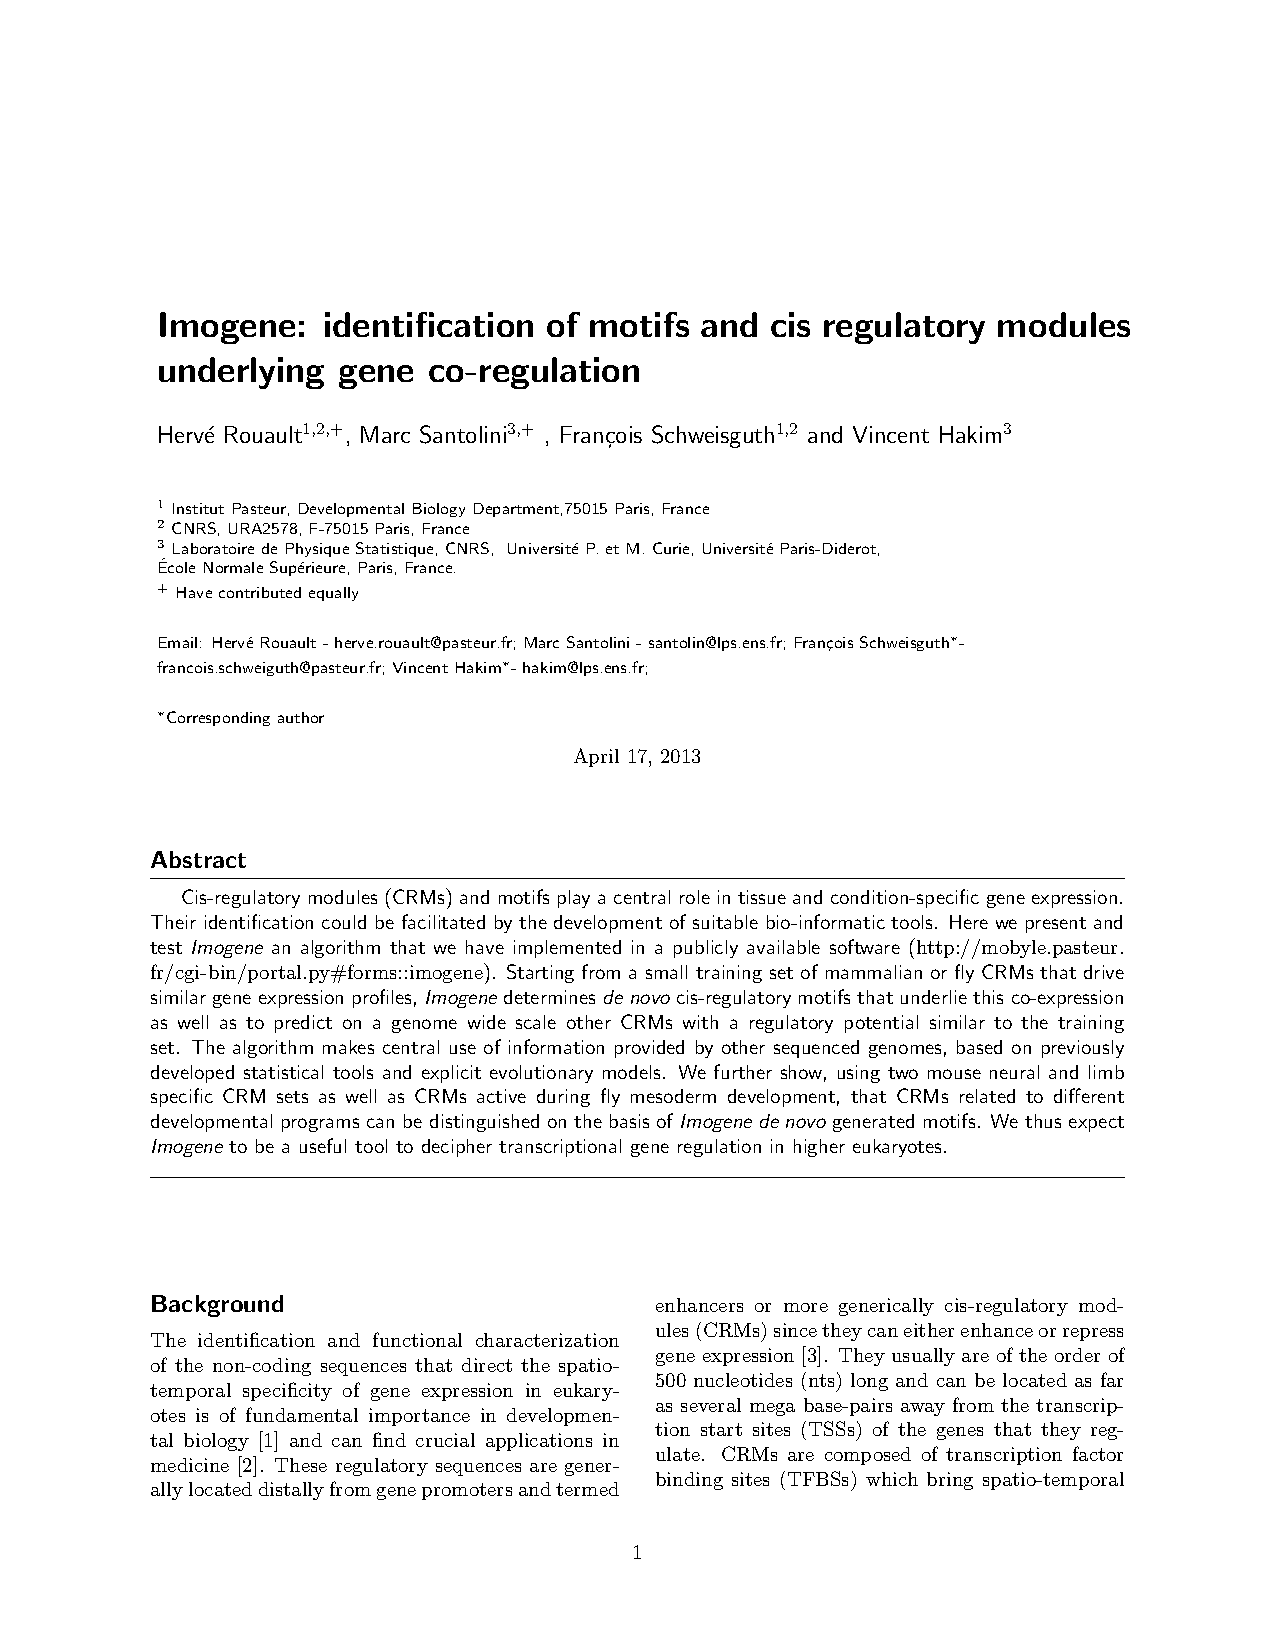
\includepdf[pages=-]{articles/imogene-genomebiol.pdf}
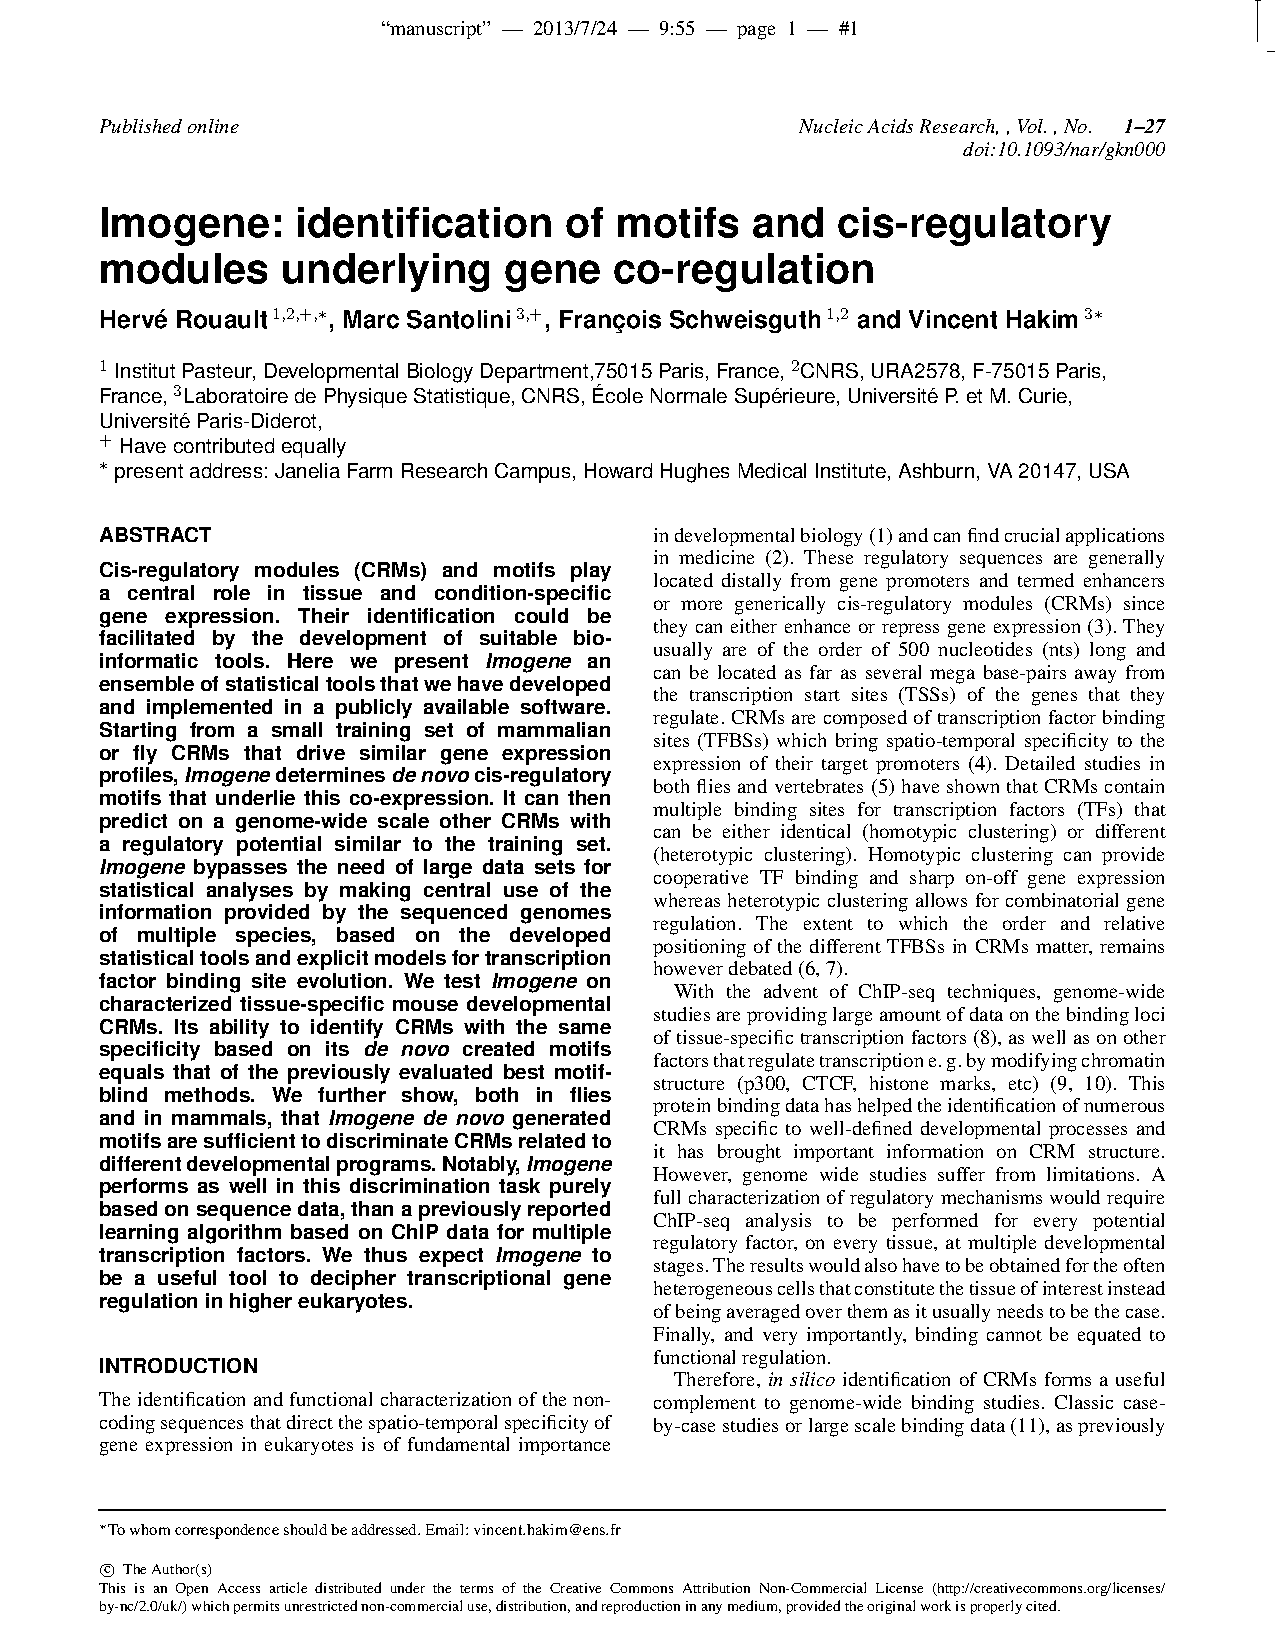
\includepdf[pages=-]{articles/manuscript-nar/manuscript.pdf}


% section article (end)

\section{Calcul de la moyenne de la post�rieure par une m�thode MCMC} 
\label{sec:calcul_de_la_moyenne_de_la_post_rieure_par_une_m_thode_mcmc}

Nous avons voulu savoir si l'approximation r�alis�e par Imogene lors du calcul
du maximum de l'estimateur de la post�rieure modifi�e (obtenue avec un prior de
Dirichlet de param�tres $\alpha_b+1$) donnait un r�sultat effectivement proche
du calcul de la moyenne de l'estimateur de la post�rieure non modifi�e (avec un
prior de Dirichlet de param�tres $\alpha_b$) :

\begin{equation}
    \underset{w_i}{\text{argmax}}\, \mathcal{L}(\{\mathcal{A}\}|w_i)\text{Dir}(w_i,\alpha_b+1) \simeq \int w_i\mathcal{L}(\{\mathcal{A}\}|w_i)\text{Dir}(w_i,\alpha_b) \text{d}w_i
\end{equation}

o� $w_i$ est le vecteur de poids de la PWM � la position $i$, $\{\mathcal{A}\}$
est l'ensemble des alignements de nucl�otides observ�s � cette position dans
les sites de fixation, $\mathcal{L}(\{\mathcal{A}\}|w_i)$ d�note la
vraisemblance de l'alignement connaissant le vecteur de poids $w_i$ et
$\text{Dir}(w_i,\alpha_b)$ est le prior de Dirichlet de param�tres $\alpha_b$.
Pour des distances phylog�n�tiques nulles ou infinies, cette approximation est
valide, et pour des distances interm�diaires, elle semble fonctionner dans le
cas simplifi� de l'arbre en �toile de la figure S$5$ de l'article. Qu'en
est-t-il dans le cas r��l avec un arbre � la topologie plus complexe?
L'estimation directe de la moyenne de cette distribution est difficile, puisque
nous n'avons pas de moyen simple de l'�chantillonner. Afin de contourner ce
probl�me, nous avons eu recours � une m�thode de Monte-Carlo par cha�nes de
Markov ou MCMC bas�e sur l'algorithme de
Metropolis-Hastings~\cite{krauth2006statistical}. Nous pr�sentons la
comparaison de la moyenne de la post�rieure obtenue par l'approche MCMC et du
maximum de la post�rieure modifi�e par descente de gradient sur un cas r�el
simple en utilisant l'arbre des vert�br�s (figure $2$ de l'article) et le
mod�le d'�volution \textit{Felsenstein}.


\subsection{Principe de l'algorithme de Metropolis-Hastings}
\label{sub:principe_de_l_algorithme_de_metropolis_hastings}

L'algorithme de Metropolis-Hastings
\cite{metropolis1953equation,hastings1970monte} permet d'�chantillonner une
distribution donn�e en utilisant le parcours d'une cha�ne de Markov ayant cette
distribution pour loi stationnaire. Un tel processus de Markov est d�fini par
des probabilit�s de transition $P(w \to w')$ entre deux �tats $w$ et $w'$. Il
converge vers une distribution stationnaire $\pi(w)$ unique sous deux
conditions : (1) les transitions sont r�versibles et le processus satisfait le
bilan d�taill� $\pi(w)P(w\to w') = \pi(w')P(w'\to w)$, (2) le processus est
ergodique, \cad que tout �tat est et reste accessible.  L'algorithme de
Metropolis-Hastings repose sur la construction d'une cha�ne de Markov ayant ces
propri�t�s et dont la distribution d'�quilibre $\pi(w)$ est la probabilit� que
l'on cherche � �chantillonner $P(w)$. Pour cela, on part de l'�quation du bilan
d�taill�, que l'on peut �crire 

\begin{equation}
    \label{eq:bilan-detaille}
    \frac{P(w \to w')}{P(w' \to w)} = \frac{P(w')}{P(w)}
\end{equation}

La transition $P(w \to w')$ est ensuite d�compos�e en deux sous-�tapes, la
proposition (\textit{proposal}) et l'acceptation (\textit{acceptance}) : 

\begin{equation}
    P(w \to w') = \underbrace{g(w \to w')}_{\text{proposition}} \cdot \underbrace{A(w\to w')}_{\text{acceptation}}
\end{equation}

En ins�rant dans l'�q. \ref{eq:bilan-detaille} on obtient

\begin{equation}
    \frac{A(w \to w')}{A(w' \to w)} = \frac{P(w')}{g(w \to w')} \frac{g(w' \to w)}{P(w)}
\end{equation}

Plusieurs choix de la fonction d'acceptation sont possibles pour satisfaire
cette �quation \cite{hastings1970monte}. Un choix courant, dit choix de
Metropolis,  est :

\begin{equation}
    \label{eq:acceptance}
    A(w \to w') = \min\left(1, \frac{P(w')}{g(w \to w')} \frac{g(w' \to w)}{P(w)}\right)
\end{equation}

On remarque que cette quantit� est invariante sous multiplication de la
distribution $P(w)$ par un facteur non nul. Autrement dit, la distribution n'a
pas besoin d'�tre normalis�e. Dans un cadre bay�sien, cela veut dire que l'on
peut remplacer la post�rieure par le produit de la vraisemblance et du
\textit{prior}.\\

La m�thode de Metropolis-Hastings se
r�sume donc ainsi :

\begin{enumerate}
\item Initialiser $w$ � une certaine valeur.
\item Choisir un nouvel �tat $w'$ tir� selon $g(w \to w')$
\item Accepter l'�tat avec une probabilit� donn�e par $A(w \to w')$. Si le nouvel �tat n'est pas accept�, alors $w'=w$.
\item It�rer jusqu'� convergence
\end{enumerate}

Au final, $w$ �tant tir� selon la distribution $P(w)$, sa moyenne est estim�e
en sommant les poids $w(t)$ obtenus au cours des $N$ it�rations r�alis�es :

\begin{equation}
    \langle w \rangle \simeq \hat{w}_N = \frac{1}{N} \sum_{t=1}^N w(t)
\end{equation}

Quant au crit�re de convergence, une possibilit� est d'utiliser le Th�or�me
Central Limite (TCL). Celui-ci stipule que la moyenne de $n$ variables
al�atoires ind�pendantes et identiquement distribu�es selon une loi de moyenne
$\mu$ et d'�cart-type $\sigma$ tous deux de valeurs finies suit, pour $n$
grand, une loi normale de moyenne $\mu$ et d'�cart-type $\sigma/\sqrt{n}$. Dans
l'approche MCMC, les �chantillons successifs $w_i$ ne sont pas ind�pendants
� cause du fait qu'on les tire selon la loi $g(w\to w')$. Il faut donc calculer
le temps de d�corr�lation $T$ pour lequel $\langle w(t) w_i(t+T) \rangle \simeq
0$, puis utiliser les �chantillons $w(t)$ obtenus toutes les $T$ it�rations
comme variables ind�pendantes.  L'application du TCL permet alors d'arr�ter les
it�rations lorsqu'une certaine pr�cision d�sir�e est atteinte, par exemple
lorsque $\sigma / \sqrt{n} < 0.05 \cdot \mu$, \cad lorsque les variations de
l'estimateur de la moyenne sont de l'ordre de $5\%$ de la valeur de la moyenne.
L'�cart-type $\sigma$ �tant lui m�me estim� � partir des �chantillons de
l'algorithme, il faut aussi s'assurer qu'il a converg� vers une valeur
stable pour appliquer le TCL.

%Il est aussi possible, comme nous le verrons par la suite,
%d'utiliser une borne inf�rieure connue � cet �cart-type.



% subsection principe_de_l_algorithme_de_metropolis_hastings (end)

\subsection{Application au calcul de la post�rieure}
\label{sub:application_au_calcul_de_la_post_rieure}

Dans notre cas, nous souhaitons utiliser l'algorithme de Metropolis-Hastings
pour calculer la valeur moyenne du vecteur de poids $w_i$ en
position $i$ de la PWM selon la distribution post�rieure
$\mathcal{P}(w_i|\{\mathcal{A}\})$:

\begin{equation}
    \langle w_i \rangle = \int w_i \mathcal{P}(w_i|\{\mathcal{A}\}) \text{d}w  %\simeq \sum_{t=1}^N w_i(t)
\end{equation}

Il nous faut pour cela d�finir une loi de proposition $g(w_i \to w_i')$
pertinente. Dans notre cas, les poids $w_i$ doivent rester dans le simplexe de
dimension $3$ d�fini par $w_A, w_C, w_G >0$ et $w_A+w_C+w_G <1$, le poids $w_T$
�tant enti�rement d�termin� par $w_T=1-w_A-w_C-w_G$.  La distribution naturelle
poss�dant cette propri�t� est la loi de Dirichlet $\text{Dir}(\al)$, de
param�tres $\al=\{\al_A,\al_C,\al_G,\al_T\}$ et de densit� de probabilit�

\begin{equation}
    f(w) = \frac{1}{B(\alpha)} \prod_{b\in \{A,C,G,T\}} w_{i,b}^{\al_b - 1}
\end{equation}

o� $B(\al)$ est la fonction b�ta multinomiale permettant la normalisation.
Cette distribution est la m�me que celle obtenue dans le cas d'observations
ind�pendantes (cf article). Afin d'acc�l�rer l'�chantillonnage MCMC, nous avons
cherch� � r�gler les param�tres $\al$ de mani�re � �tre au plus proche de la
distribution $\mathcal{P}(w_i|\{\mathcal{A}\})$. Dans le cas de $N$ sites
ind�pendants, celle-ci suit une loi de Dirichlet de param�tres $\al_p + N_i$,
o� $\al_p$ est le vecteur de pseudo-counts et $N_i$ le vecteur donnant les
nombres d'observations des nucl�otides en position $i$ au sein des diff�rentes
s�quences. Dans le cas d'un arbre phylog�n�tique corr�lant les s�quences, le
nombre \textit{effectif} d'observation est moins grand que le nombre total de
s�quences.  Nous avons donc d�fini les param�tres de notre proposition
comme �tant

\begin{equation}
    \al_b = \al_p + N_{\text{eff}}\cdot w_i
\end{equation}

o� $N_{\text{eff}}=N_{\text{sites}}\cdot N_{\text{spe}} /2$ avec
$N_{\text{sites}}$ le nombre d'alignements observ�s et $N_{\text{spe}}$ le
nombre d'esp�ces dans l'alignement ($12$ dans les deux cas, \droso et
mammif�res).  Grossi�rement, cela revient � dire que le mod�le d'�volution
r�duit d'un facteur $2$ le nombre de s�quences ind�pendantes. Nous avons
calcul� que le taux d'acceptation (proportion de mouvements propos�s qui sont
accept�s)  pour ce param�tre �tait de l'ordre de $50\%$, une valeur
g�n�ralement consid�r�e comme raisonnable~\cite{krauth2006statistical}. Nous
obtenons finalement l'expression pour la proposition :


\begin{equation}
    \label{eq:proposal}
    g(w \to w') = \frac{1}{B(\alpha)} \prod_{b\in \{A,C,G,T\}} (w_{i,b}')^{\al_{p,b} + N_{\text{eff}}\cdot w_{i,b}  - 1}
\end{equation}

Le vecteur $w_i$ est initialis� � la valeur qu'il prendrait si toutes les
s�quences orthologues �taient des observations ind�pendantes  (cf article) :

\begin{equation}
    w_{i,b}(0) = w_{i,b}^\text{inde} = \frac{N_{i,b} + \al_b}{N_{\text{tot}} + \sum_b \al_b}
\end{equation}


Le poids $w_i(1)$ suivant est tir� selon la probabilit� de transition
$g(w_i(0) \to w_i(1))$. Les diff�rentes quantit�s de l'�quation
\ref{eq:acceptance} sont ensuite calcul�es et la transition est accept�e avec
probabilit� $A\left(w_i(0) \to w_i(1)\right)$. 
\\

%Reste le probl�me de la convergence. Nous avons vu dans la section pr�c�dente
%que l'on pouvait utiliser le th�or�me centrale limite pour d�cider de la
%convergence. 
%Dans notre cas, nous poss�dons une borne inf�rieure de
%l'�cart-type $\sigma$ de la post�rieure :  celui-ci est donn� par l'�cart-type
%$\sigma_{\text{inde}}$ du cas limite o� les s�quences sont des observations
%ind�pendantes. En effet, dans ce cas limite le nombre d'observations est plus
%grand qu'avec un mod�le d'�volution, et la d�viation standard est donc plus
%petite. Notant $\al_{i,b}^\text{inde}=N_{i,b}+\al_b$ et
%$\al_0=\sum_b\al_{i,b}^{\text{inde}}$, celle-ci s'�crit

%\begin{equation}
    %\sigma_{\text{inde}} = \sqrt{\frac{\al_{i,b}^\text{inde}(\al_0-\al_{i,b}^\text{inde}}{\al_0^2(\al_0+1)}} 
%\end{equation}
%Le TCL peut alors �tre appliqu� en utilisant des �chantillons ind�pendants de
%$w_i$ (voir paragraphe suivant
%\ref{sub:illustration_de_la_m_thode_mcmc_sur_un_exemple}). Notre crit�re de
%convergence est que l'�cart absolu maximum obtenu entre l'estimation de la
%moyenne � l'it�ration courante et les $10$ pr�c�dentes estimations doit �tre
%plus petit que $\sigma_{\text{inde}}/\sqrt{n}$, o� $n$ est le nombre
%d'�chantillons ind�pendants.



% subsection application_au_calcul_de_la_post_rieure (end)


\subsection{Illustration sur un exemple}
\label{sub:illustration_de_la_m_thode_mcmc_sur_un_exemple}

%\bfig
%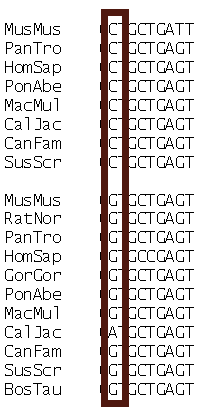
\includegraphics[width=0.2\textwidth]{figures/MCMC/TFBS.pdf}
%\captionbf{Sites utilis�s pour le MCMC}{

    %La position �tudi�e est celle encadr�e, contenant au total $10$ G, $8$ C et
    %$1$ A.

%}
%\label{fig:MCMC/TFBS}
%\efig

%\bfig
%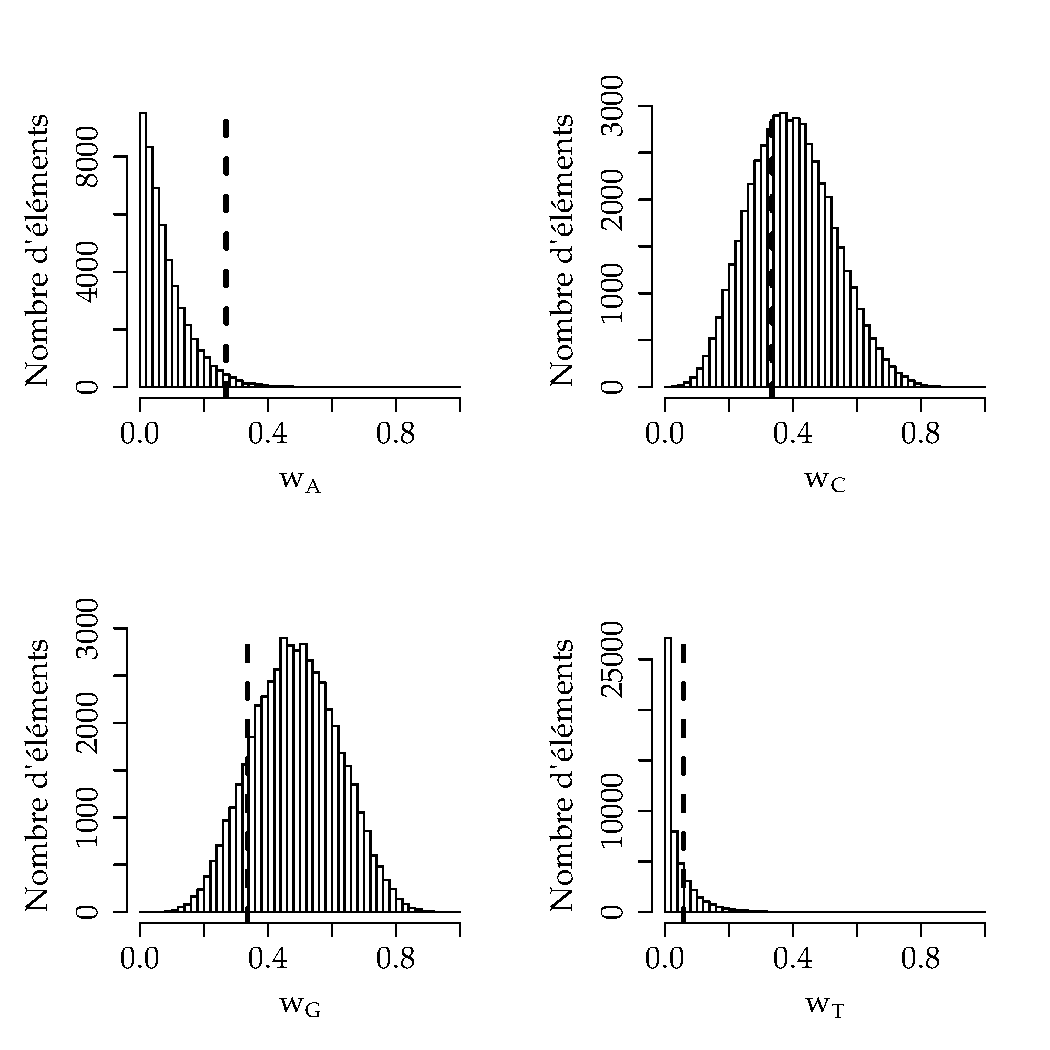
\includegraphics[width=0.5\textwidth]{figures/MCMC/plotDirichlet.pdf}
%\captionbf{Distribution de la fonction de proposition $g(w_i^\text{inde} \to w)$}{

    %La distribution de Dirichlet est r�alis�e pour $50,000$ tirages al�atoires,
    %avec un bin de $0.02$. Les lignes verticales en pointill�s indiquent
    %l'estimation de la moyenne obtenue apr�s convergence (voir
    %fig.~\ref{fig:MCMC/plotConvergence}).

%}
%\label{fig:MCMC/plotDirichlet}
%\efig

\bfig
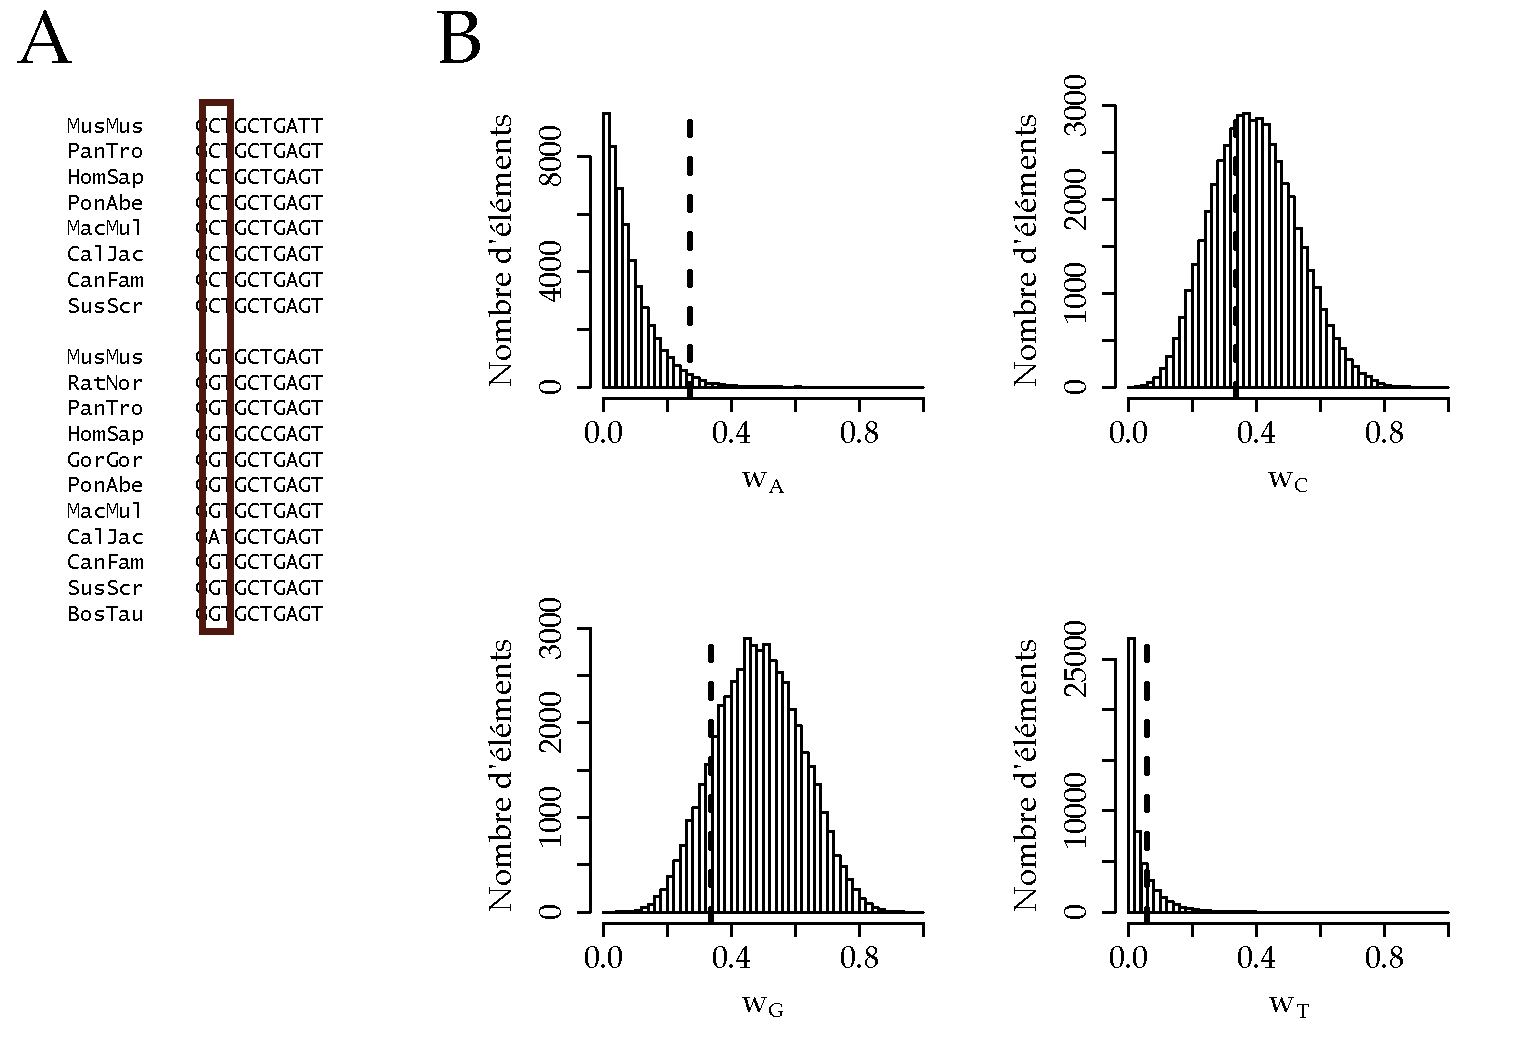
\includegraphics[width=1\textwidth]{figures/MCMC/sites-dirichlet.pdf}
\captionbf{Conditions initiales}{

    (A) Sites utilis�s pour le MCMC. On s'int�resse ici � la $2$�me position,
    contenant au total $10$ G, $8$ C et $1$ A.

    (B) Distribution de la distribution de Dirichlet correspondant � la
    proposition $g(w_i^\text{inde} \to w)$. L'�chantillonnage consiste en
    $50,000$ tirages al�atoires, et le bin est de $0.02$. Les lignes verticales
    en pointill�s indiquent l'estimation de la moyenne obtenue apr�s
    convergence (voir fig.~\ref{fig:MCMC/var_cv}).

}
\label{fig:MCMC/sites-dirichlet}
\efig

�tudions maintenant un exemple concret. Nous pr�sentons la m�thode sur le cas
pr�sent� en fig.~\ref{fig:MCMC/sites-dirichlet}A et nous utilisons le mod�le
d'�volution \textit{Felsenstein}. Le vecteur de poids $w_i$ est initialis� au
cas ind�pendant $w_i^\text{inde}$. La proposition $g(w_i^\text{inde} \to w)$
(�q.~\ref{eq:proposal})  est montr�e en fig.~\ref{fig:MCMC/sites-dirichlet}B.
On voit notamment comment la distribution de Dirichlet permet de rester dans le
simplexe dans les cas $w_A$ et $w_T$ proches de $0$. La valeur finale de
l'estimation de la moyenne de la post�rieure obtenue apr�s convergence de la
cha�ne (voir ci-dessous) est aussi montr�e : elle est relativement proche de la
moyenne de la distribution, indiquant que le choix de la valeur initiale est
effectivement judicieux.  \\


%\bfig
%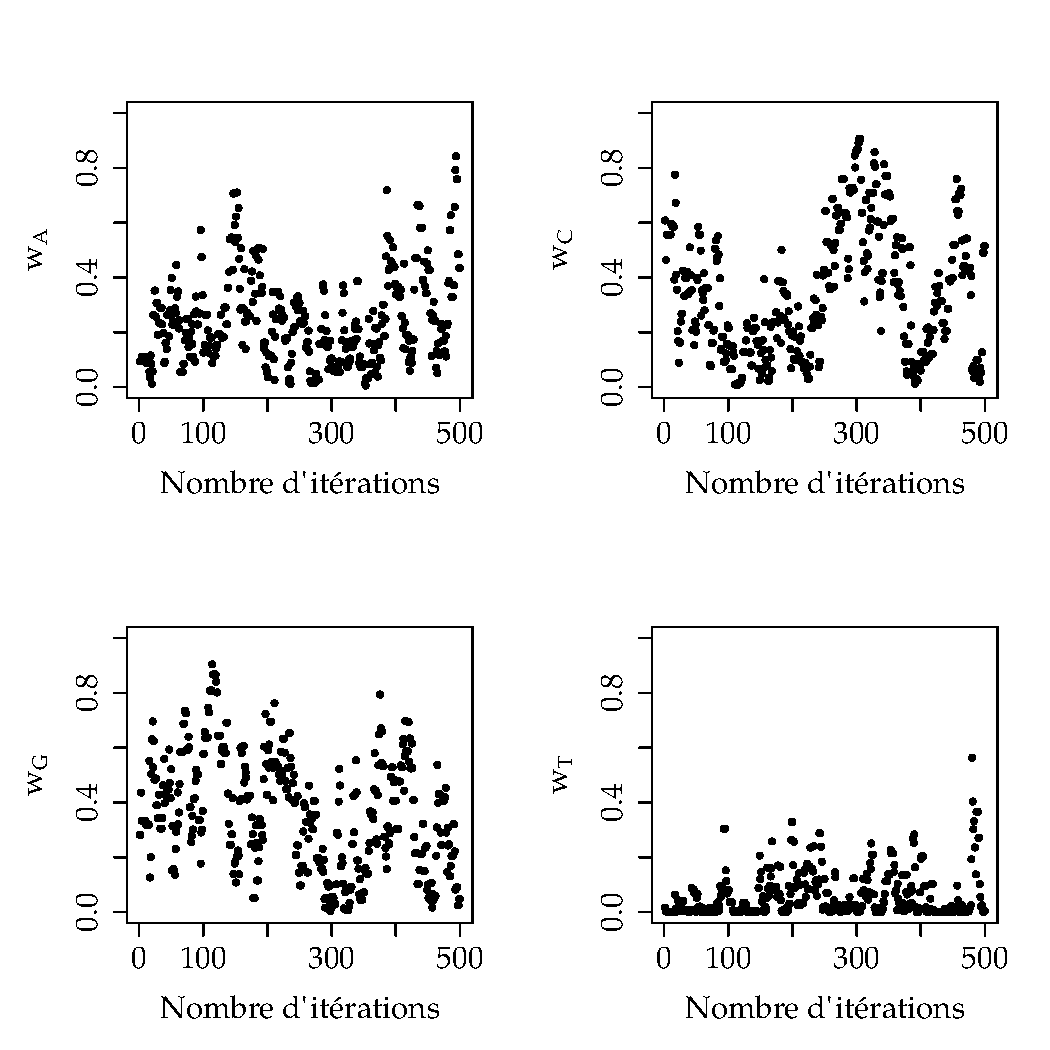
\includegraphics[width=0.5\textwidth]{figures/MCMC/plotSampling.pdf}
%\captionbf{Extrait de l'�chantillonnage de $w_i$}{

%Les $500$ premiers �chantillons $w_i$ de la cha�ne MCMC sont montr�s.

%}
%\label{fig:MCMC/plotSampling}
%\efig

%\bfig
%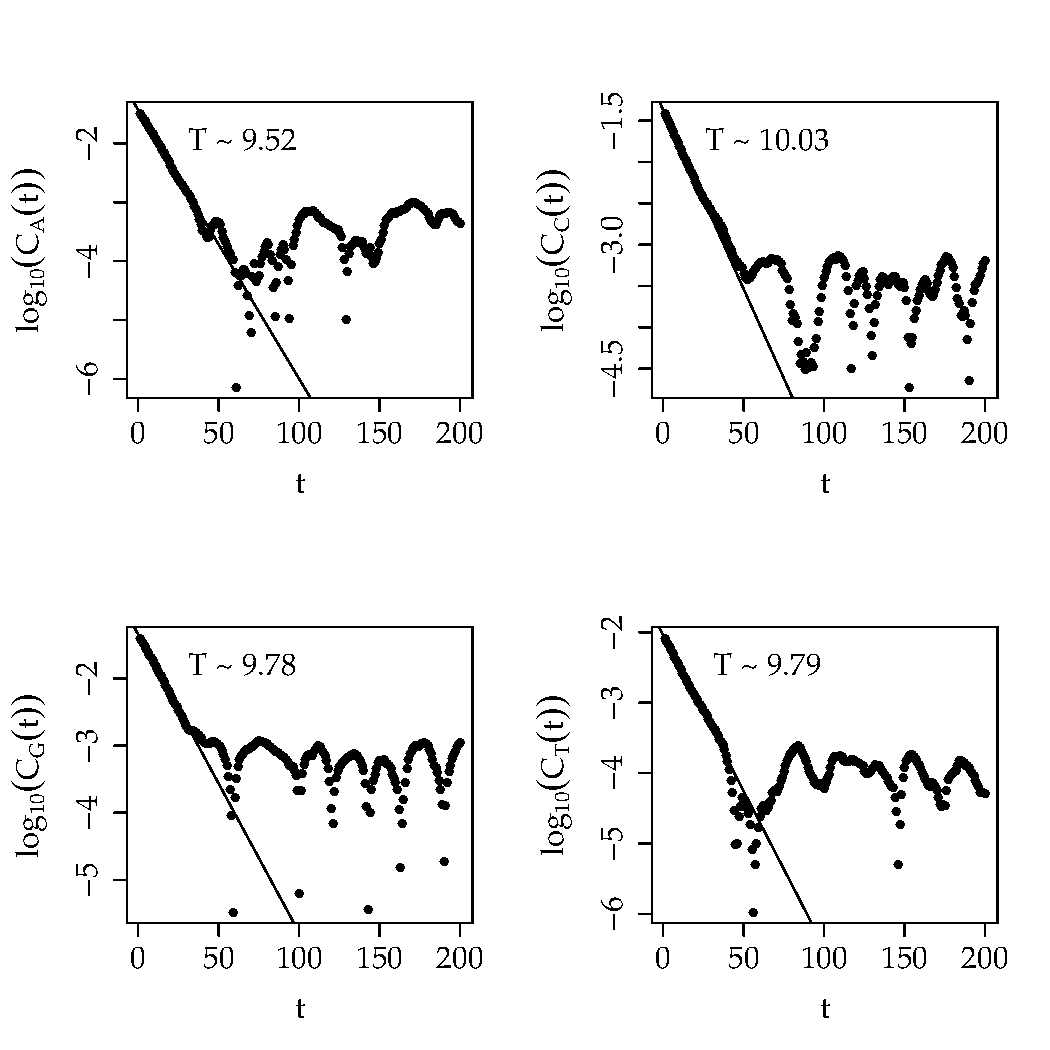
\includegraphics[width=0.5\textwidth]{figures/MCMC/plotAutocorr.pdf}
%\captionbf{Fonction d'auto-corr�lation de la cha�ne MCMC}{

%Corr�lation entre des �chantillons s�par�s de $t-1$ it�rations. Une droite est
%ajust�e sur les $20$ premi�rs points, permettant de recueillir
%la pente $-T_b$ donnant le temps de d�corr�lation.

%}
%\label{fig:MCMC/plotAutocorr}
%\efig

\bfig
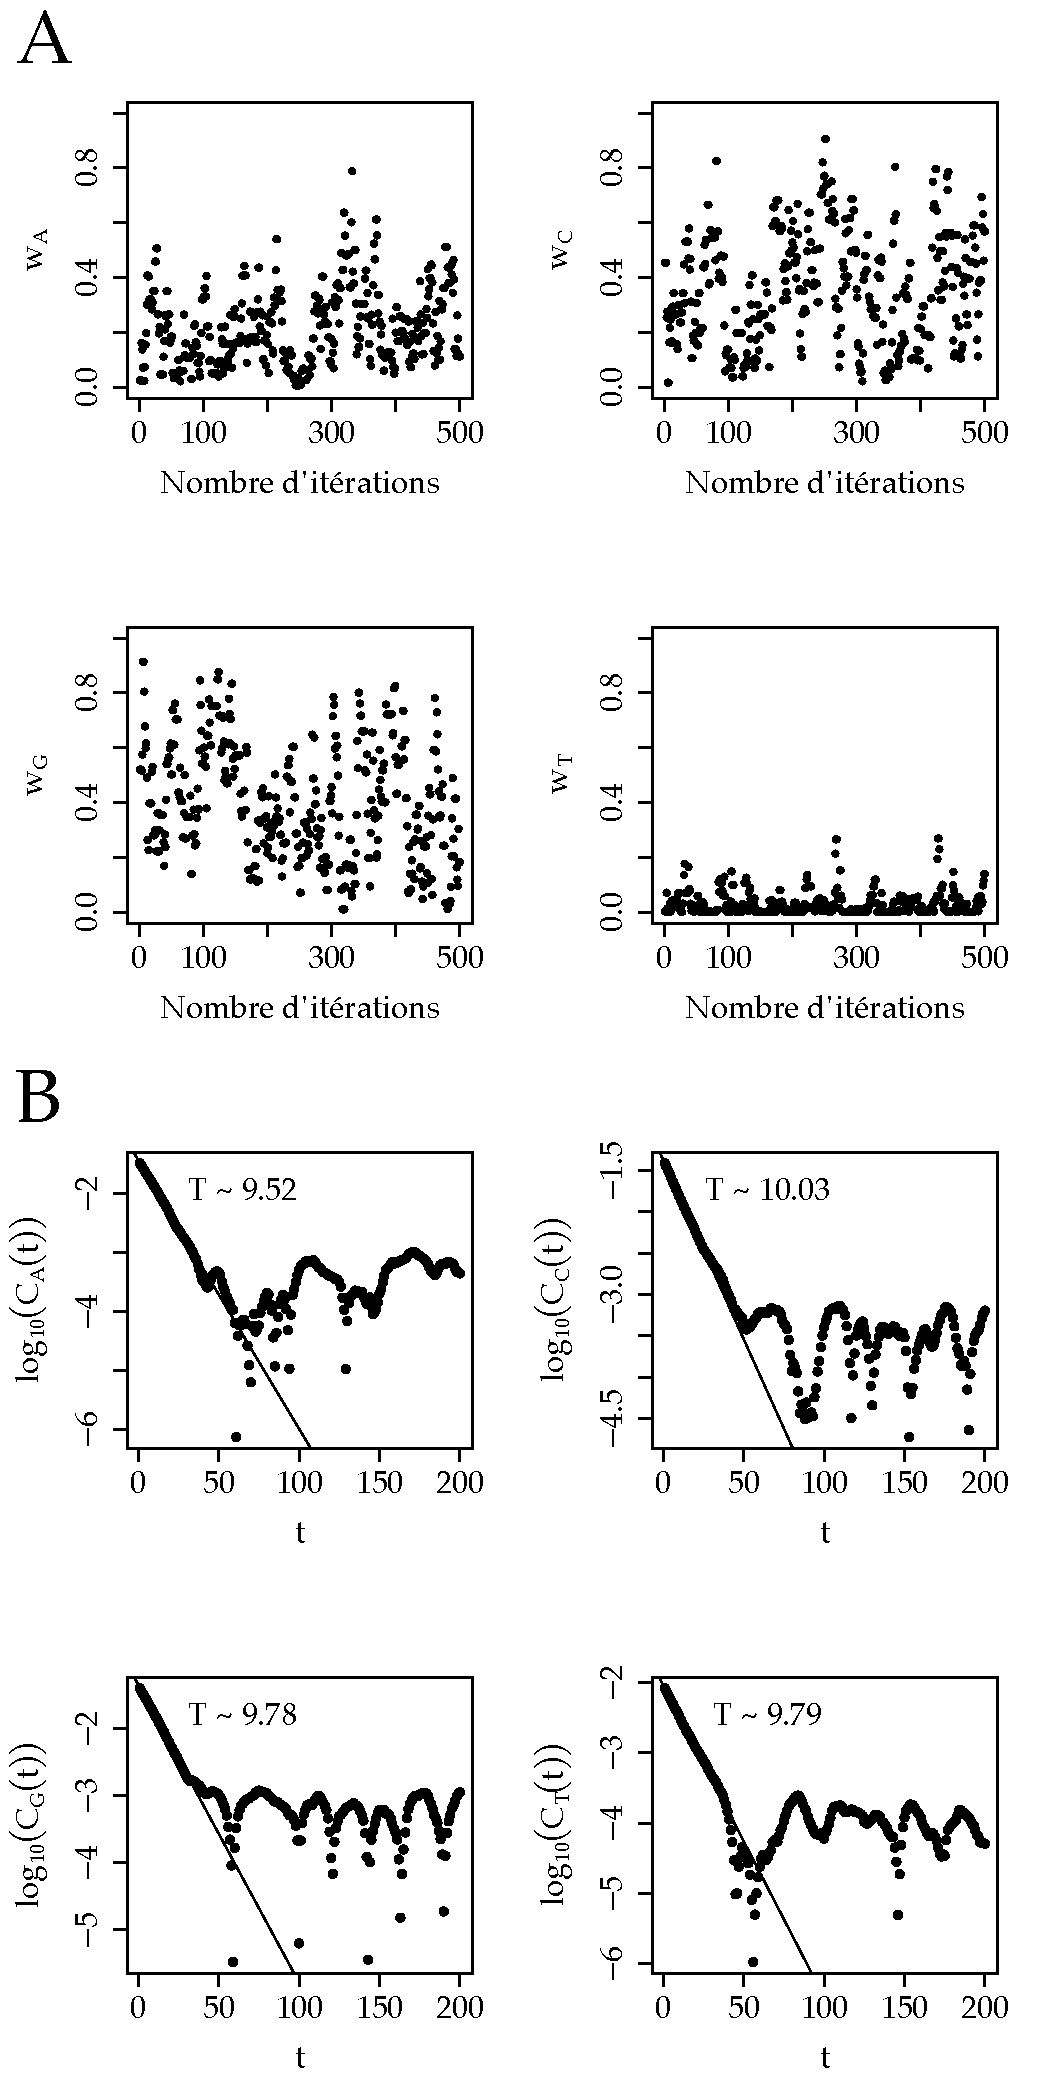
\includegraphics[width=0.6\textwidth]{figures/MCMC/sampling-autocorr.pdf}
\captionbf{Corr�lations entre les �chantillons}{

(A) Extrait de l'�chantillonnage de $w_i$. Les $500$ premiers �chantillons
$w_i$ de la cha�ne MCMC sont montr�s.

(B) Fonction d'auto-corr�lation de la cha�ne MCMC. La corr�lation $C_b(t)$ est
r�alis�e entre des �chantillons s�par�s de $t-1$ it�rations. Une droite est
ajust�e sur les $20$ premi�rs points, permettant d'obtenir la pente $-T_b$
donnant le temps de d�corr�lation.

}
\label{fig:MCMC/sampling-autocorr}
\efig

La cha�ne MCMC est ensuite lanc�e. Le taux d'acceptation est calcul� comme
valant $62\%$. Les $500$ premiers �chantillons de $w_i$ sont montr�s en figure
\ref{fig:MCMC/sampling-autocorr}A. On note que certains points sont
corr�l�s : diminutions ou augmentations successives de la valeur courante
$w_i(t)$ sur plusieurs it�rations. Pour quantifier cet effet, nous avons mesur�
la corr�lation temporelle des �chantillons. Celle-ci est donn�e par

\begin{equation}
    C_b(\tau) = \frac{1}{N} \sum_{t=1}^{N-\tau} w_{i,b}(t) w_{i,b}(t+\tau) - \left(\frac{1}{N}\sum_{t=1}^N w_{i,b}(t)\right)^2
\end{equation}

avec dans ce cas $N=50,000$. Le logarithme de cette quantit� est montr�e en
figure \ref{fig:MCMC/sampling-autocorr}B. L'int�r�t du logarithme est de mettre
en exergue le caract�re exponentiel de la d�corr�lation
%\footnote{D'apr�s le
%th�or�me de Perron-Froebenius, le temps de d�correlation d'une cha�ne de Markov
%est donn� par $T=-1/\log(\mu)$, o� $\mu$ est la valeur propre de la cha�ne de
%Markov de plus grande valeur absolue} 
:

\begin{equation}
    C_b(\tau) \propto e^{-\tau/T_b}
\end{equation}

Les temps de d�correlation $T_b \sim 10$ sont estim�s en ajustant une droite
sur les $20$ premiers points de la courbe. Maintenant que l'on connait le temps
de corr�lation entre deux �chantillons, il est possible d'obtenir des
�chantillons ind�pendants en les choisissant � des intervalles plus grands que
$T_b$. Dans notre cas, nous avons choisis un intervalle de $30$ it�rations.  \\

\bfig
%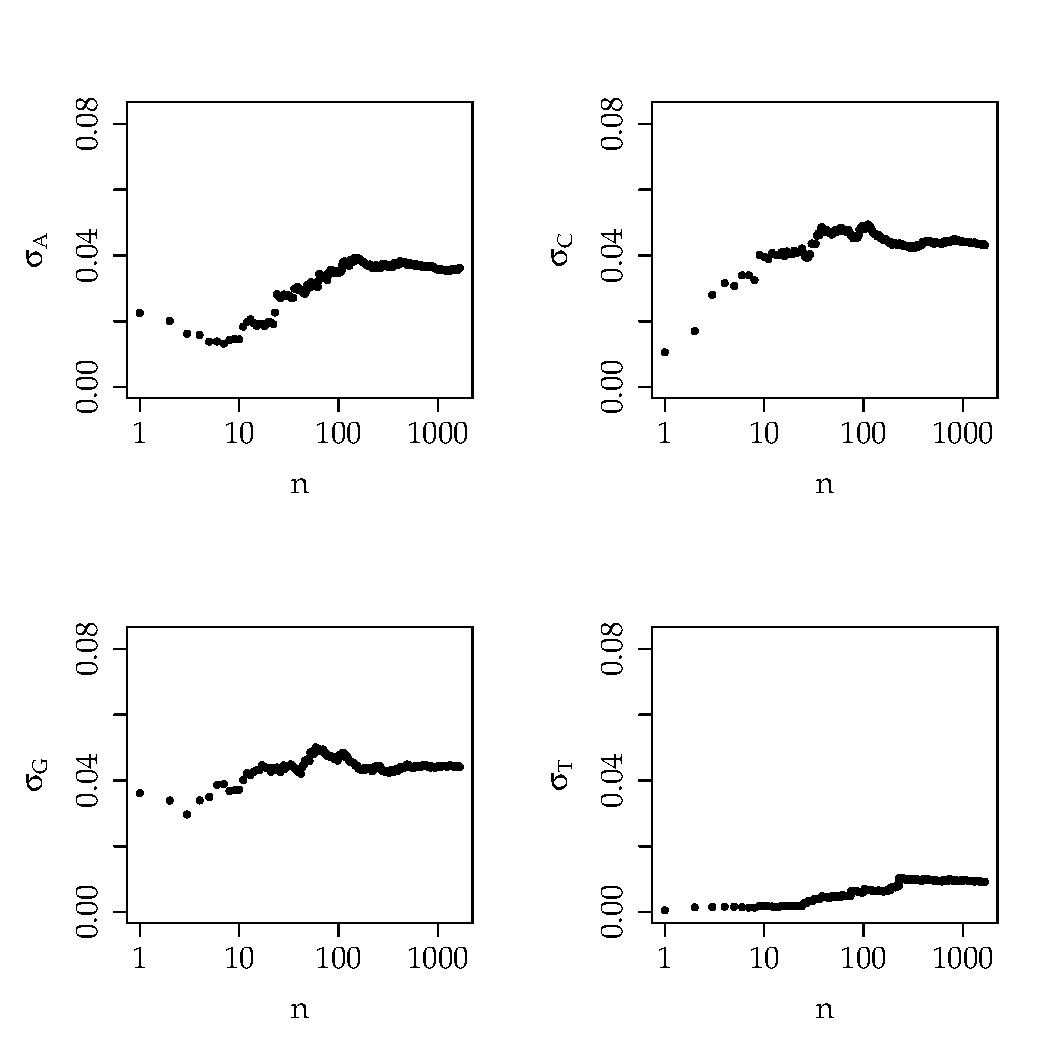
\includegraphics[width=0.5\textwidth]{figures/MCMC/plotCVvar.pdf}
%\includegraphics[width=0.5\textwidth]{figures/MCMC/plotConvergence.pdf}
\includegraphics[width=0.55\textwidth]{figures/MCMC/var-cv.pdf}
\captionbf{Estimation de la convergence}{

   
    
    (A) �cart-type $\sigma_b$ de la distribution $w_{i,b}$ estim� � partir de
    $n$ �chantillons ind�pendants. Ces �chantillons sont pris toutes les $30$
    it�rations au sein de la cha�ne MCMC, soit environ $3$ fois le temps de
    d�corr�lation. On observe qu'au bout de $100$ it�rations l'�cart-type est
    stabilis�. Par ailleurs les fluctuations sont relativement faibles, au plus
    de l'ordre de $\sim 10\%$ de la moyenne.

    (B) La convergence est estim�e gr�ce au Th�or�me Centrale Limite.
    L'�cart-type de l'estimateur de la moyenne se comporte comme  $\sigma_b
    / \sqrt{n}$. La pr�cision demand�e correspond � un �cart-type $\leq 5\%$ de
    la moyenne pour les $4$ bases, ce qui correspond � l'intersection la plus
    tardive entre les courbes noire et grise (dans notre cas le cadran du bas
    � droite).

}
\label{fig:MCMC/var_cv}
\efig

Nous souhaitons maintenant �tudier la convergence de la cha�ne MCMC. Pour cela,
nous utilisons le Th�or�me Central Limite (TCL, cf
\ref{sub:principe_de_l_algorithme_de_metropolis_hastings}).  Pour un  nombre
$n$ suffisamment grand d'�chantillons ind�pendants, l'�cart-type de la
distribution de l'estimateur empirique de la moyenne $\hat{w}_n$ se comporte
comme $\sigma_b / \sqrt{n}$, o� $\sigma_b$ est l'�cart-type de la distribution
$\mathcal{P}(w_i|\mathcal{A})$. Ce dernier doit lui-m�me �tre estim� � partir
de la cha�ne MCMC. Nous pr�sentons en figure \ref{fig:MCMC/var_cv}A la valeur
de l'estimation $\sigma_b(n)$ obtenue pour $n$ it�rations ind�pendantes. On
voit que cette valeur atteint rapidement en $\sim100$ it�rations une valeur
stable, et que dans tous les cas les fluctuations sont faibles, de l'ordre de
$10\%$ de $\hat{w}_n$. Il para�t donc raisonnable d'utiliser cette valeur de
$\sigma_b$ pour le TCL. Nous tra�ons en figure \ref{fig:MCMC/var_cv}B la
quantit� $\sigma_b(n)/\sqrt{n}$. La cha�ne est consid�r�e comme converg�e
lorsque cette valeur est inf�rieure ou �gale � $5\%$ de la valeur moyenne
estim�e $\hat{w}_n$ (ligne grise) dans les $4$ cas.  Ce seuil est bien entendu
arbitraire et d�pend de la pr�cision voulue par l'utilisateur sur l'estimation.
N�anmoins, une plus grande pr�cision implique un plus long temps de calcul.  \\

Nous comparons en figure \ref{fig:MCMC/plotConvergenceCompare} la valeur de
l'estimation du Maximum A Posteriori (MAP) de la post�rieure modifi�e (voir
article) obtenue avec la m�thode de descente de gradient et celle de la moyenne
de la post�rieure obtenue avec l'approche MCMC, en fonction du nombre total
d'it�rations.  L'approche MCMC  converge vers un �tat proche de celui donn� par
la descente de gradient, On note que la convergence de l'approche MCMC est
beaucoup plus lente : plus de $10,000$ it�rations, alors que la descente de
gradient n'en requiert que $100$. Au vu de la faible diff�rence entre les deux
r�sultats, nous utilisons dans Imogene l'approche de maximisation de la
post�rieure modifi�e, ce qui permet un gain de temps consid�rable pour
l'algorithme (au minimum un facteur $10$).


\bfig
\includegraphics[width=1\textwidth]{figures/MCMC/plotConvergenceCompare.pdf}
\captionbf{Comparaison des approches par MCMC et par descente de gradient}{

L'approche de maximisation de (l'oppos� de) la post�rieure modifi�e par
descente de gradient (rouge, cf article) est compar�e � l'approche de calcul de
la moyenne de la post�rieure par MCMC (noir). Les deux m�thodes sont
initialis�es au m�me $w_i^{\text{inde}}$. Alors que la m�thode par descente de
gradient converge rapidement ($\sim100$ it�rations), l'approche MCMC converge
plus lentement, dans ce cas plus de $10,000$ it�rations. Au final les deux
approches convergent vers des quantit�s proches (lignes pointill�es rouges et
noires). 

}
\label{fig:MCMC/plotConvergenceCompare}
\efig

% subsection illustration_de_la_m_thode_mcmc_sur_un_exemple (end)


% section calcul_de_la_moyenne_de_la_post_rieure_par_une_m_thode_mcmc (end)

\FloatBarrier
\section{Conclusion et perspectives du chapitre \thechapter}

Nous avons pr�sent� Imogene, un algorithme bay�sien utilisant la phylog�nie de
recherche de motifs et modules conduisant une r�gulation commune. Imogene est
bas� sur l'algorithme introduit par \citet{Rouault2010p327} dans le cas des
Drosophiles, et l'�tend au cas des mammif�res. Nous avons pr�sent� des tests
d'Imogene sur des CRMs poss�dant une expression d�termin�e chez l'embryon de
souris (tube neural et bourgeon de membre), et avons montr� la capacit�
d'Imogene de pr�dire des CRMs conduisant � une expression similaire au sein de
s�quences interg�niques.  Parmi les motifs g�n�r�s par Imogene, certains sont
associ�s � des r�gulateurs connus des �tapes du d�veloppement consid�r�es.  Par
ailleurs, nous avons montr� que les motifs g�n�r�s par Imogene pouvaient �tre
utilis�s pour g�n�rer un classifieur lin�aire permettant d'associer un CRM
donn� � une classe li�e � une expression sp�cifique. Ce classifieur montre des
performances similaires � un classificateur bas� sur des donn�es biologiques
spatio-temporelles extensives~\cite{Zinzen2009p760}, mais ne n�cessite que la
connaissance de quelques s�quences de chaque classe et fournit en plus la
connaissance des motifs r�gulateurs.  \\

Imogene peut �tre utilis� � partir de l'interface Mobyle de l'Institut
Pasteur~\url{http://mobyle.pasteur.fr/cgi-bin/portal.py#forms::imogene}. Nous
esp�rons ainsi qu'il pourra servir � des biologistes souhaitant mettre � jour
des r�gulateurs putatifs dans des CRMs fonctionnels et d�tecter dans le g�nome
des CRMs poss�dant une activit� similaire.



\newpage

%%%%%%%%%%%%%%%%%%%%%%%%%%%%%%%%%%%%%%%%%%%%%%%%%%%%%%%%%%%%%%%%%%%%%%%%%%%%%%%%%%%%%%%%%%%
\chapter{\ChTrichomes}
\label{ch:trichomes}
\minitoc
\newpage
\section*{Introduction du chapitre \thechapter}

Nous pr�sentons maintenant une application de Imogene au cas de la
diff�renciation des trichomes (poils) chez la Drosophile, r�alis�e en
collaboration avec l'�quipe de Serge Plaza � l'Universit� Paul Sabatier.
Plusieurs motifs ont �t� g�n�r�s � partir de $14$ CRMs connus pour r�guler le
processus de diff�renciation des trichomes. Parmi les motifs g�n�r�s, deux
d'entre eux ont montr� une meilleure capacit� � distinguer les CRMs positifs de
l'ensemble d'apprentissage de CRMs n�gatifs. Le crit�re de distinction est bas�
sur l'optimisation de Pareto, caract�risant la satisfaction de plusieurs
contraintes � la fois. Dans notre cas, les contraintes sont de maximiser le
nombre de CRMs positifs trouv�s par les motifs (maximisation de la sensibilit�)
tout en minimisant le nombre de faux positifs (maximisation de la sp�cificit�).
Ces crit�res d�finissent une fronti�re de Pareto de motifs optimum. En variant
les diff�rents param�tres de Imogene, nous avons trouv� deux motifs sur la
fronti�re de Pareto. Parmi les deux motifs, l'un d'eux (\og svbf7 \fg)
correspond au r�gulateur ma�tre du processus de diff�renciation des trichomes,
et l'autre (\og blue motif\fg) est un motif nouveau. L'importance des deux
motifs pour la r�gulation est montr�e par mutagen�se. Par ailleurs, ces motifs
permettent de distinguer des \chipseq pour \textit{svb} li�s � une r�gulation
(dont le g�ne le plus proche subit une perte d'expression lors du KO de
\textit{svb}) des \chipseq ne l'�tant pas. Ce travail montre donc un exemple de
la possibilit� d'utiliser Imogene sur sun un petit ensemble (ici $14$ CRMs) de
donn�es biologiques fonctionnelles pour d�tecter des motifs nouveaux et
fonctionnels.

\newpage

\section{Concept d'optimum de Pareto} 
\label{sec:concept_d_optimum_de_pareto}

Dans l'article qui suit, nous utilisons le principe d'optimum de Pareto, li�
� la satisfaction simultan�e de plusieurs contraintes. Le probl�me est le
suivant. �tant donn�s $14$ CRMs positifs li�s � une m�me r�gulation de la
diff�renciation des trichomes chez l'embryon de Drosophile, et $25$ CRMs
n�gatifs ne conduisant aucune expression au stade de d�veloppement consid�r�,
quels motifs permettent le mieux de distinguer les deux classes? Le probl�me
est similaire � celui de \textit{pattern recognition} introduit dans l'article
pr�c�dent en section \ref{sec:article_imogene}. N�anmoins, nous avons ici
adopt� une d�marche l�g�rement diff�rente. 

Des motifs sont appris sur les CRMs positifs pour diff�rents seuils $S_g$
(variant entre $7$ et $13$ bits). Ces motifs sont ensuite utilis�s pour pr�dire
les CRMs positifs parmi les CRMs initiaux. Un CRM est d�clar� comme positif
s'il contient au moins  $n$ sites conserv�s ($n=1$, $2$, ou $3$) au-dessus d'un
seuil $S_s$ (variant entre $7$ et $13$ bits). Pour des param�tres $S_g$, $n$ et
$S_s$ donn�s, un motif d�tectera un nombre FP de Faux Positifs (les CRMs
n�gatifs qui sont pr�dits positifs) et omettra un nombre FN de Faux N�gatifs
(les CRMs positifs qui ne sont pas pr�dits comme tels). L'optimisation de
Pareto consiste � trouver les param�tres $S_g$, $n$ et $S_s$ qui minimisent
� la fois FP et FN. Il est possible de minimiser diff�rentes fonctions de co�t
pour FP et FN, attribuant des poids plus ou moins importants � l'une ou l'autre
des contraintes. Dans notre cas, nous avons d�fini l'optimum de Pareto comme
minimisant la fonction $|\text{FN}+\text{FP}|$.  La droite
$|\text{FN}+\text{FP}|=cte$ contenant les meilleurs optima de Pareto pour les
diff�rents motifs est la fronti�re de Pareto. 

Dans notre cas, deux des motifs g�n�r�s sont sur la fronti�re de Pareto : le
motif svbF7 et le motif bleu (fig.~\ref{fig:plaza/pareto/plot_pareto}), pour
$S_g=10$ bits, $n=1$, $S_s=8.5$ bits. Ce sont par ailleurs les $2$ premiers
motifs g�n�r�s � ce seuil. Les $3$ motifs suivants sont montr�s en gris. Le
motif svbF7 correspond au TF \textit{svb} (\textit{Shavenbaby}), r�gulateur
ma�tre de la diff�renciation des trichomes. Le motif OvoQ6 correspond � la PWM
de Transfac pour \textit{svb}, et n'apporte pas une aussi bonne classification
que svbF7. Le motif bleu, quant � lui, n'est pas connu. Nous montrons aussi le
motif jaune, introduit dans l'article, qui n'est pas pr�dit par Imogene mais
correspond � un motif de r�gulation ultra-conserv� dans les de diff�rentes
esp�ces de drosophiles~\cite{Elemento2005fk}, et poss�dant un r�le fonctionnel
investigu� par mutagen�se.


\bfig
\includegraphics[width=1\textwidth]{figures/plaza/pareto/plot_pareto.pdf}
\captionbf{Fronti�re d'efficacit� de Pareto}{

    Illustration de l'optimisation de Pareto permettant la s�lection des
    param�tres lors de la g�n�ration de motifs. Ici, nous voulons � la fois
    minimiser le nombre de Faux Positifs (FP) et le nombre de Faux n�gatifs
    (FN).  Diff�rents motifs sont successivement utilis�s pour classer les
    s�quences comme positives ou n�gatives, une s�quence �tant d�clar�e comme
    positive pour un motif si elle contient au moins $n$ sites conserv�s
    au-dessus d'un seuil $S_s$. Les diff�rents points correspondent aux
    diff�rentes performances. Un l�ger bruit a �t� ajout� aux points pour
    rendre visibles ceux qui sont superpos�s (fonction \texttt{jitter} de R,
    param�tre \texttt{factor}$=0.5$). Le motif svbF7 et le motif bleu sont tous
    deux optimaux pour des param�tres bien d�finis $S_g=10$ bits, $n=1$,
    $S_s=8.5$ bits : ils dessinent la fronti�re de Pareto $|FP+FN|=cte$ en
    pointill�s bruns.

}
\label{fig:plaza/pareto/plot_pareto}
\efig




% section concept_d_optimum_de_pareto (end)


%%%%%%%%%%%%%%%%%%%%%%%%%%%%%%%%%%%%%%%%%%%%%%%%%%%%%%%%%%%%%%%%%%%%%%%%%%%%%%%%%%%%%%%%%%%%%%%%%%%	%%%%%%%%%%%%%%%%%%%%%%%%%%%%%%%%%%%%%%%%%%%%%%%%%%%%%%%%%%%%%%%%%%%%%%%%%%%%%%%%%%%%%%%%%%%%%%%%%%%	

\newpage
\section{Article} 
\label{sec:article_plaza}

\includepdf[pages=-]{articles/trichomes-genomebiol/Menoret_et_al_GenBiol_revised.pdf}
\includepdf[pages=-]{articles/trichomes-genomebiol/Figures_rev_S.pdf}
\includepdf[pages=-]{articles/trichomes-genomebiol/Menoret_SupInfos_revised.pdf}
\includepdf[pages=-]{articles/trichomes-genomebiol/Menoret_et_al_FigSupLegend_revised.pdf}
\includepdf[pages=-]{articles/trichomes-genomebiol/FigSup_rev_S.pdf}

% section article (end)
			
%%%%%%%%%%%%%%%%%%%%%%%%%%%%%%%%%%%%%%%%%%%%%%%%%%%%%%%%%%%%%%%%%%%%%%%%%%%%%%%%%%%%%%%%%%%%%%%%%%%	%%%%%%%%%%%%%%%%%%%%%%%%%%%%%%%%%%%%%%%%%%%%%%%%%%%%%%%%%%%%%%%%%%%%%%%%%%%%%%%%%%%%%%%%%%%%%%%%%%%	
\newpage	
			

\section{Conclusion et perspectives du chapitre \thechapter}

Imogene a �t� appliqu� sur un ensemble d'apprentissage compos� de $14$ CRMs
r�gulant la diff�renciation des trichomes chez l'embryon de Drosophile. Les
diff�rents param�tres (seuils de g�n�ration, de d�tection) ont �t� optimis�s
par une approche de Pareto visant � maximiser le nombre de CRMs positifs
pr�dits par les motifs tout en minimisant le nombre de CRMs n�gatifs pr�dits
parmi un ensemble de $25$ CRMs n'ayant aucune activit� au stade de
d�veloppement consid�r�. Deux motifs ont �t� trouv� par cette approche : le
motif svbF7 correspondant � \textit{svb}, le r�gulateur ma�tre de la
diff�renciation des trichomes, et un nouveau motif, le motif bleu, que nous
n'avons pas pu associer � un motif connu. 

La validit� de ces motifs a �t� montr�e par mutagen�se (figures $3$, $4$ et $5$
de l'article). Par ailleurs, ces motifs sont pr�dictifs des \chipseq de
\textit{svb} fonctionnels, \cad ceux qui sont associ�s � un g�ne dont
l'expression diminue chez les mutants \textit{svb} (figure S$5$). Les CRMs
fonctionnels poss�dent une grande vari�t� de grammaire des sites de fixation
(figures $5$ et $7$ de l'article), un r�sultat similaire � celui obtenu par
\citet{Zinzen2009p760} dans le cas de la diff�renciation de diff�rents tissus
chez l'embryon de drosophile. Plusieurs entr�es (combinaisons de TFs) m�nent
� une sortie (motif d'expression du g�ne rapporteur) similaire : cette
flexibilit� est r�miniscente du mod�le \textit{billboard} introduit en section
\ref{sub:enhanceosome_billboard}.  N�anmoins, bien qu'il soit clair que la
grammaire des sites soit diff�rente entre diff�rents CRMs, cette grammaire
semble relativement bien conserv�e au cours de l'�volution d'un CRM (figures 8,
S8A, et S8B).  Enfin, dans la plupart des cas on observe l'absence de
\textit{clustering} de motifs homotypiques sur les CRMs, bien que les motifs
soient pr�sents en plus grand nombre dans les loci des g�nes r�gul�s par
rapport � des g�nes non r�gul�s (figure S$2$). Une explication possible est que
'abondance de sites dans l'environnement du CRM permet d'augmenter localement
la concentration du TF pour faciliter son recrutement \invivo au niveau des
CRMs poss�dant des sites de forte affinit�.

Il serait � pr�sent int�ressant de caract�riser plus en avant le motif bleu
g�n�r� par l'approche \denovo. Une possibilit� serait d'utiliser la technique
de simple hybride pr�sent�e en
\ref{sub:approche_clonale_la_technique_de_simple_hybride} afin d'identifier la
prot�ine associ� au motif bleu, en utilisant comme app�t les prot�ines connues
de la drosophile et comme proie le site consensus du motif bleu.

 


\newpage

%%%%%%%%%%%%%%%%%%%%%%%%%%%%%%%%%%%%%%%%%%%%%%%%%%%%%%%%%%%%%%%%%%%%%%%%%%%%%%%%%%%%%%%%%%%
\chapter{\ChMuscle}
\label{chap:muscle}
\minitoc
\newpage
\section*{Introduction du chapitre \thechapter}

Cette derni�re partie est consacr�e � l'�tude de la diff�renciation musculaire.
Ce travail a �t� effectu� en collaboration avec l'�quipe de Pascal Maire
� l'Institut Cochin, qui m'a accueilli et m'a permis de r�aliser une partie des
exp�riences pr�sent�es, avec l'aide de Iori Sakakibara. Nous nous int�ressons
ici particuli�rement aux hom�oprot�ines Six$1$ et Six$4$ (\textit{Sine Oculis
Homeobox Homolog} $1$ et $4$, r�f�r�es dans la suite par \sixd) qui sont des
\tfs impliqu�s dans la r�gulation des stades successifs de la myogen�se. Ils
activent en effet les TFs n�cessaires � l'engagement de cellules pluripotentes
dans la voie myog�nique et � leur diff�rentiation : Pax3 (\textit{Paired Box
$3$}) ainsi que les Facteurs de R�gulation Myog�nique Myf5 (\textit{Myogenic
Factor $5$}), Mrf4 (\textit{Muscle-Specific Regulatory Factor $4$}, aussi
appel� Myf$6$), Myod (\textit{Myogenic Differentiation}) et Myog
(\textit{Myogenin}). Cette r�gulation passe par la fixation des prot�ines Six
sur un site \mef d'environ $10$bp. 

Nous nous sommes d'abord int�ress� aux cibles transcriptionnelles de \sixd
� l'�chelle du g�nome, ainsi qu'� leurs cor�gulateurs. Pour cela, nous avons
d'abord r�alis� un mod�le PWM des sites \mef, que nous avons utilis� pour la
pr�diction de sites. Nous avons par ailleurs r�cup�r� de nombreuses donn�es
relatives � la diff�renciation musculaire : \chipseq de TFs et des marques
�pig�n�tiques des histones, donn�es d'expression de type RNAseq, sites de
fixation conserv�s que nous avons obtenus par analyse bioinformatique, etc. Ces
donn�es ont �t� regroup�es sur le visualiseur de UCSC, permettant d'envisager
facilement le contexte de r�gulation de certains g�nes d'int�r�t. Nous
pr�sentons plusieurs validations de pr�dictions obtenues par analyse
bioinformatique avec ces donn�es.

Par ailleurs, nous nous sommes int�ress� � l'action concert�e ou
\textit{synergie} entre \sixd et le TF ma�tre MyoD au cours de la
diff�renciation musculaire. Nous avons trouv� un certain nombre de CRMs fix�s
par MyoD et poss�dant un site \mef conserv� chez les mammif�res, et dont le
g�ne le plus proche n'est activ� qu'en pr�sence de MyoD et de \sixd. Parmi les
g�nes en question figurent \myog, TF requis pour la diff�renciation terminale,
et des g�nes structuraux comme \textit{Tnnc1} (\textit{Troponin C Type $1$}) ou
\textit{Ttn} (\textit{Titin}). Nous avons test� l'activit� des CRMs pr�dits et
en avons trouv� $70\%$ qui r�capitulent l'expression du g�ne le plus proche
lorsqu'ils sont test�s par transfection avec un rapporteur Lucif�rase. Nous
avons par ailleurs utilis� Imogene pour pr�dire des cor�gulateurs et avons
test� l'importance des sites par mutagen�se.

%%%%%%%%%%%%%%%%%%%%%%%%%%%%%%%%%%%%%%%%%%%%%%%%%%%%%%%%%%%%%%%%%%%%%%%%%%%%%%%%%%%%%%%%%%%%%%%%%%%	%%%%%%%%%%%%%%%%%%%%%%%%%%%%%%%%%%%%%%%%%%%%%%%%%%%%%%%%%%%%%%%%%%%%%%%%%%%%%%%%%%%%%%%%%%%%%%%%%%%	
\newpage

\section{Introduction � la myogen�se squelettique} 
\label{sec:introduction_la_myogen_se}

\subsection{Les diff�rentes �tapes de la myogen�se}
\label{sub:les_diff_rentes_tapes}

La myogen�se correspond � la formation des tissus musculaires, ceux-ci �tant
regroup�s en trois types majeurs : les muscles cardiaques, les muscle lisses et
les muscles squelettiques. C'est la formation de ces derniers qui nous
int�resse ici. Les muscles squelettiques sont compos�s de fibres musculaires polynucl�es
provenant de la fusion de prog�niteurs musculaires appel�s myoblastes. Ils sont
sous le contr�le du syst�me nerveux central, et composent l'un des organe
majeur des vert�br�s, concentrant $\sim40\%$  du poids corporel. La
myogen�se squelettique d�bute relativement t�t au cours de l'embryogen�se : � $8.5$
jours\footnote{La mi-journ�e correspondant au fait que la f�condation a lieu la
nuit.} apr�s f�condation (ou E$8.5$ pour \textit{Embryonic day} $8.5$) chez
l'embryon de souris sur un total de $18$ jours embryonnaires. Elle a lieu au
niveau des somites, structures p�riodiques situ�es au niveau des futures
vert�bres (fig.~\ref{fig:buckingham-myogenesis}a). Les �tapes de fusion des
myoblastes et de maturation des fibres s'�talent ensuite sur toute
l'embryogen�se (fig.~\ref{fig:buckingham-myogenesis}b), ainsi que dans le
muscle adulte lors de la r�g�n�ration musculaire \cite{Parker2003p761}.

\bfigp
\includegraphics[width=.9\textwidth]{figures/buckingham-myogenesis.pdf}
\captionbf{Formation du muscle squelettique chez l'embryon de souris}{

    Figure tir�e de \citet{Buckingham2007p776} illustrant les diff�rentes
    �tapes de la myogen�se. (a) Le dermomyotome �pith�lial d'un somite (vert)
    ainsi que le muscle squelettique du myotome (beige) sont d'abord form�s par
    la d�lamination des cellules provenant des extr�mit�s du dermomyotome
    (fl�ches bleues) : c'est la premi�re vague de la myogen�se. Ensuite, lors
    d'une deuxi�me vague, le dermomyotome central perd sa structure �pith�liale
    et des cellules musculaires prog�nitrices s'int�grent au myotome
    (fl�ches rouges). Les TFs pr�curseurs de ces �v�nements sont indiqu�s en
    rouge. (b) Sch�ma montrant les �tapes de diff�renciation des prog�niteurs
    musculaires, ainsi que les temps de d�veloppement associ�s (E : jour
    embryonnaire).

}
\label{fig:buckingham-myogenesis}
\efigp


% subsection les_diff_rentes_tapes (end)

\subsection{Les Facteurs de R�gulation Myog�nique et leurs cofacteurs}
\label{sub:la_r_gulation_g_n_tique_les_facteurs_de_r_gulation_myog_nique_ou_mrfs}

%\bfig
%\includegraphics[width=1\textwidth]{figures/bentzinger_myogenesis_tfs.pdf}
%\captionbf{Small caption for Table of Figures}{

%Main caption

%}
%\label{fig:bentzinger_myogenesis_tfs}
%\efig

D'un point de vue g�n�tique, la myogen�se des vert�br�s est coordonn�e en
partie par l'action de $4$ Facteurs de R�gulation Myog�nique (MRF pour
\textit{Myogenic Regulatory Factors}) : MyoD, Myf5, Mrf4 et Myog, qui font
partie de la famille de prot�ines \textit{basic Helix-Loop-Helix} (bHLH) et se
fixent sur les bo�tes E (ou E-box) du type CANNTG.  Ces MRFs sont activ�s
successivement � travers une cascade de r�gulation g�n�tique, et se r�gulent les
uns les autres. Par exemple, Myf5, MRF4 et MyoD peuvent activer MyoD ; Myf5,
MyoD et Mrf4 r�gulent l'expression de Myog ; et Myog peut activer l'expression
de Mrf4 \cite{Naidu1995uq}. En outre, MyoD et Myog peuvent s'auto-activer
\cite{Thayer1989kx}. Enfin, un certain degr� de redondance a �t� observ� entre
Myf5, Mrf4 et MyoD au cours du d�veloppement embryonnaire de la souris, et
l'analyse des embryons KO pour ces g�nes a conduit � la conclusion qu'ils ont
tous la capacit� d'activer la myogen�se � partir de cellules embryonnaires
pluripotentes et d'agir comme des g�nes de d�termination
\cite{KassarDuchossoy2004p823}. 


Ces MRFs sont la cl� de vo�te de la diff�renciation myog�nique. Cependant, la
r�gulation pr�cise du r�seau de g�nes activ�s par les MRFs n�cessite leur
coop�ration avec d'autres facteurs de transcription. En particulier, la liaison
de MyoD � l'ADN n'est pas pr�dictive d'une activit� enhancer
\cite{Cao2010p1805}. Ainsi, \citet{Molkentin1996p646} ont montr� que
l'activation transcriptionnelle par les MRFs est renforc�e par la fonction des
TFs � bo�te MADS MEF$2$. Leur importance a ult�rieurement �t� confirm�e par les
travaux de \citet{Blais2005p809} : en utilisant un grand nombre de g�nes cibles
des MRFs, les auteurs ont cherch� dans leur r�gion promotrice des sites de
liaison sur-repr�sent�s pour les TFs issus de la base de donn�es Transfac. Ils
ont ainsi constat� que l'�l�ment riche en A/T reconnu par MEF2 �tait parmi eux,
et ont confirm� son recrutement � plusieurs de ces sites.  Par ailleurs, un
autre motif d'ADN trouv� comme sp�cifiquement enrichi parmi les promoteurs
cibles des MRFs �tait l'�l�ment \mef (consensus GAAACCTGA), le site de liaison
des hom�oprot�ines Six. Cette s�quence \mef �tait particuli�rement abondante au
sein des promoteurs des g�nes dont l'expression �tait induite de mani�re
significative au cours de la diff�renciation.
% subsection
% la_r_gulation_g_n_tique_les_facteurs_de_r_gulation_myog_nique_ou_mrfs (end)



\subsection{Les hom�oprot�ines Six}
\label{sub:les_hom_oprot_ines_six}

Les hom�oprot�ines Six associ�es aux sites MEF$3$ poss�dent un r�le �tendu au
cours de la myogen�se, et nous en pr�sentons maintenant les d�tails.  Parmi les
6 g�nes appartenant � la famille des hom�oprot�ines Six
  (fig.~\ref{fig:kawakami-six-expression}), \textit{Six$1$} et \textit{Six$4$}
  ont re�u une attention particuli�re dans le contexte de la myogen�se
  squelettique, bien que d'autres membres comme \textit{Six$2$} ou
  \textit{Six$5$} semblent �tre en mesure de compenser partiellement leur perte
  \cite{Relaix2013ve}. Ces deux g�nes se trouvent � proximit� l'un de l'autre
  sur le chromosome $12$ de la souris et sont s�par�s par $100$kb de s�quence
  interg�nique. L'�quipe de Pascal Maire a d�j� identifi� plusieurs fonctions
  cl�s de \textit{Six$1$} dans le lignage musculaire au cours de
  l'embryogen�se, par l'analyse de mod�les de souris d�pourvues de
  \textit{Six$1$} (Six$1$KO) et de Six$1$ et Six$4$ (\sixdko), et par des
  exp�riences de \chip.  L'analyse des embryons \sixdko \cite{Grifone2005vn}
  � E$10$ \cite{Niro2010p3444} et E$18$ \cite{Richard2011ys} a permis
  d'identifier des cibles g�n�tiques directes et indirectes de Six$1,4$, et
  a d�voil� plusieurs fonctions des hom�oprot�ines Six pendant le d�veloppement
  musculaire et la sp�cialisation des fibres musculaires.  

\bfig
\includegraphics[width=.75\textwidth]{figures/kawakami-six-expression.pdf}
\captionbf{Motifs d'expression et localisation g�nomique des g�nes de la famille Six}{

    Figure tir�e de \cite{Kawakami2000bh}, montrant les motifs d'expression des
    g�nes de la famille Six chez l'embryon (A) et dans l'oeil (B) � E$13.5$.
    Les couleurs similaires refl�tent des motifs d'expression similaires. La
    localisation chromosomique des g�nes est aussi montr�e en (C). 

}
\label{fig:kawakami-six-expression}
\efig


Les principaux points sont les suivants (fig.~\ref{fig:muscle/myogenese_six})
: Six$1$ et Six$4$ sont requis pour la gen�se des prog�niteurs myog�niques
hypaxiaux (\cad ventraux).  En l'absence de Six$1$ et Six$4$, les cellules
ventrales pluripotentes du dermomyotome somitique ne parviennent pas � adopter
un destin de prog�niteur myog�nique et elles n'expriment ni \textit{Pax3} ni
les MRFs. Six$1$ et Six$4$ contr�lent directement l'expression de
\textit{Pax$3$} \cite{Grifone2007p728}, et donc l'engagement des cellules
pluripotentes dermomyotomales dans un destin de prog�niteur myog�nique.  Plus
tardivement, l'expression de \textit{Myf$5$} dans le membre est contr�l�e par
un enhancer \og membre \fg li� par les prot�ines Six$1$ et Six$4$, et cette
liaison est n�cessaire pour permettre l'expression de Myf$5$
\cite{Giordani2007p473}. Par ailleurs, deux enhancers contr�lent sp�cifiquement
l'expression de MyoD au cours de l'embryogen�se et au cours de la r�g�n�ration
du muscle adulte: le \textit{Distal Regulatory Region} ou DRR
\cite{Asakura1995ly} et le \textit{Core Enhancer} ou CE
\cite{Kucharczuk1999zr}. La liaison de ces �l�ments par Six$1$ et Six$4$ a �t�
confirm�e par \chip au cours de l'embryogen�se (\citet{Relaix2013ve}, voir
section \ref{sub:r_gulation_de_myod1_par_les_prot_ines_six}) ainsi que dans des
cultures de cellules satellites \cite{Le-Grand2012qf}, qui sont des cellules
souches du muscle adulte activ�es lors de la r�g�n�ration musculaire.
L'expression de Mrf$4$ n'est pas d�tect�e chez les embryons \sixdko � E$10$
\cite{Grifone2007p728}. Myog est aussi sous le contr�le direct des prot�ines
Six \cite{Spitz1998p3285}. Enfin, les prot�ines Six r�gulent des g�nes
sp�cifiques des fibres glycolytiques de type rapide (voir section
\ref{sub:r_gulation_d_un_lincrna_par_six_dans_le_muscle_adulte}). Par exemple,
la mutation du site MEF$3$ au sein du promoteur de \textit{Aldoa}, g�ne codant
pour une enzyme impliqu�e dans la glycolyse, entra�ne l'abolition de
l'expression d'un transg�ne rapporteur dans des myofibres adultes
\cite{Spitz1997p455}.

\bfig
\includegraphics[width=1\textwidth]{figures/muscle/myogenese_six.pdf}
\captionbf{R�le des prot�ines Six au cours de la myogen�se}{

(A) Figure tir�e de \citet{Bentzinger2012ij}. La myogen�se embryonnaire
consiste en plusieurs �tapes de diff�renciation musculaire : la gen�se des
prog�niteurs embryonniques exprimant \textit{Pax3}, leur sp�cification en
myoblastes par l'induction des g�nes de d�termination myog�nique comme
\textit{Myf5} et \textit{Myod1}, la diff�renciation des myoblastes en myocytes
avec l'expression de \textit{Myog} et leur fusion en myotubes qui se
sp�cialisent plus tardivement en fibres de type lentes (oxydatives) ou rapides
(glycolytiques).  On note que les prot�ines Six sont exprim�es continuellement
au cours de ces �tapes (et aussi plus tardivement dans les fibres rapides).

(B) Les hom�oprot�ines Six  interviennent dans la r�gulation de ces diff�rentes
�tapes \invivo en r�gulant les TFs indiqu�s selon une cascade de boucles
\textit{feed-forward}. 

}
\label{fig:muscle/myogenese_six}
\efig

%Ainsi, Six$1$ et Six$4$ contr�lent directement Pax$3$ et tous les MRF, mais ce
%contr�le est spatialement (axe dorso-ventral et axe ant�ro-post�rieur)
%h�t�rog�ne dans l'embryon.




%Par analyse
%bioinformatique, j'ai trouv� deux MEF3 sites dans le noyau activateur et un
%MEF3 site du RRC.  Mutation de ces trois MEF3 des sites aboli par plus de 95%
%l'expression d'un journaliste du transg�ne MyoD dans une souris transg�nique
%essai transitoire � E11.5 dans toutes les lign�es myog�niques (tronc, membres,
%t�te) (Relaix
%2012). 


%Mutations introduites dans le site MEF3 pr�sente dans le
%promoteur myog�nine abolies expression d'une �-galactosidase transg�ne
%rapporteur myog�nine cours de l'embryogen�se (Spitz,1998), et les mutations
%introduites dans le site MEF3 pr�sente dans le promoteur AldolaseA abolis
%l'expression d'un transg�ne rapporteur dans myofibres adultes (Spitz, 1997).
%Par cons�quent, six prot�ines apparaissent comme de bons candidats pour MFR de
%modulation de la r�gulation transcriptionnelle.  N�anmoins, la coop�ration des
%centres de tri et TFS associ�s est loin d'�tre enti�rement comprise, et la
%coop�ration des centres de tri avec non pas un, mais une vari�t� de facteurs de
%transcription, par exemple � diff�rents moments au cours de l'embryogen�se,
%afficher une croissance musculaire natale et pendant la r�g�n�ration du muscle
%adulte est susceptible de se produire sur diff�rents activateurs de g�nes
%cibles.



% subsection les_hom_oprot_ines_six (end)



\FloatBarrier
% section introduction_la_myogen_se (end)

\section{Int�gration de donn�es bioinformatiques et exp�rimentales sur le muscle} 
\label{sec:integration_de_donn_es_bioinformatiques_et_exp_rimentales_sur_le_muscle}

La premi�re �tape de notre collaboration avec l'�quipe de P. Maire a �t� de
construire un mod�le de motif pour les sites de fixation \mef associ�s aux
prot�ines \sixd chez la souris. Un tel motif, qui n'existait jusqu'alors pas,
permet de r�aliser des pr�dictions pr�cises, et nous discuterons apr�s de leur
v�rification.  Par ailleurs, nous avons r�cup�r� de nombreuses donn�es
exp�rimentales dans la litt�rature sur la diff�renciation musculaire (\chipseq,
RNAseq, donn�es �pig�n�tiques\ldots) et les avons int�gr�es au syst�me de
visualisation de UCSC (pr�sent� en introduction, section
\ref{sub:outils_visualisation}).  L'int�gration de ces multiples donn�es permet
d'appr�hender facilement et rapidement les ph�nom�nes de r�gulation ayant lieu
lors de la diff�renciation musculaire � l'�chelle locale de g�nes d'int�r�t
comme � l'�chelle globale g�nomique en croisant les donn�es. 


\subsection{Obtention d'une PWM optimale pour MEF3}
\label{sub:obtention_d_une_pwm_optimale_pour_mef3}

\begin{table}[!t]
\centering
%\resizebox{8cm}{!} {
\begin{tabular}{|l|l|}
\hline
\multicolumn{2}{|c|}{S�quences positives d'apprentissage}\\
\hline
Myog & \texttt{GAAACCTGA} \\
Pax3 & \texttt{GAAATCTAA} \\
Myf5 & \texttt{GTAACTGGA} \\
Myod-DRR & \texttt{GAAACCGGA} \\
Mlc-hox & \texttt{GTAATTTAA} \\
Atp2a1-1 & \texttt{GTAACTGGA} \\
Atp2a1-2 & \texttt{GTAACCTGA} \\
Tnnc2 & \texttt{GAAATTTAA} \\
Nrk & \texttt{GCAAGGCGA} \\
Sarcalumenin & \texttt{GGAACTTGA} \\
Myl1-2 & \texttt{GAAATTGAA} \\
Ifitm3 & \texttt{GTAATTTGA} \\
Mybph-2 & \texttt{GAAATCTGA} \\
Myeov2 & \texttt{GAAACTTGA} \\
\hline
\end{tabular}
\begin{tabular}{|l|l|}
\hline
\multicolumn{2}{|c|}{S�quences positives test}\\
\hline
Aldoa & \texttt{GAAACCTGA} \\
Ato & \texttt{GTCATTTGA} \\
Kcne1l & \texttt{GATAACGGA} \\
Myf5 & \texttt{GAAATTTAA} \\
Pax3-1 & \texttt{GAAATGTAA} \\
Pax3-2 & \texttt{GTTACTGGA} \\
Pvalb & \texttt{GTAACCTGA} \\
Utrophine & \texttt{GTCACCTGA} \\
Na-K-ATPase & \texttt{GCAACCTGA} \\
Myf5-2 & \texttt{GCAACCTGA} \\
Myf5-sat & \texttt{GAAATCTGA} \\
Lbx1 & \texttt{GCCACCTGA} \\
MCK & \texttt{GACACCCGA} \\
IgfBp5 & \texttt{GCAATTTGA} \\
Troponine-C & \texttt{GTAACCTGA} \\
Sarcalumenin & \texttt{GGAACTTGA} \\
Nrk & \texttt{GCAAGGCGA} \\
Tp4 & \texttt{GCAAGCAGA} \\
\hline
\end{tabular}
%}
\captionbf{Sites \mef positifs}{ 
    
    Le tableau de gauche correspond aux $14$ sites conserv�s chez les
    mammif�res que nous avons utilis�s pour l'apprentissage de la PWM \mef, et
    le tableau de droite aux sites utilis�s comme un ensemble test ind�pendant
    de Vrais Positifs dans la courbe ROC de la figure
    \ref{fig:muscle/roc-mef3}.

}
\label{tab:mef3_pos}
\end{table}

\begin{table}[!t]
\centering
%\resizebox{8cm}{!} {
\begin{tabular}{|l|l|}
\hline
\multicolumn{2}{|c|}{S�quences n�gatives}\\
\hline
myf5-1 & \texttt{GACAGTGGA} \\
myf5-2 & \texttt{GTAACCTCA} \\
myf5-3 & \texttt{GTAACTGGG} \\
pax3-1 & \texttt{GGAACTTGA} \\
pax3-2 & \texttt{GTATTAATA} \\
pax3-3 & \texttt{GGATAAAGA} \\
pax3-4 & \texttt{GCTAATTGA} \\
pax3-5 & \texttt{GAAAGATTA} \\
pax3-6 & \texttt{GCTCTCTGA} \\
pax3-7 & \texttt{GAGCCCTGA} \\
pvalb-1 & \texttt{GCACAATGA} \\
pvalb-2 & \texttt{GCAGGCTGA} \\
unknown-1 & \texttt{GCAATCTGA} \\
unknown-2 & \texttt{GAGTCCTGA} \\
\hline
\end{tabular}
%}
\captionbf{Sites \mef n�gatifs}{ 
    
    Sites n�gatifs utilis�s comme Faux Positifs dans la courbe ROC de la figure
    \ref{fig:muscle/roc-mef3}.

}
\label{tab:mef3_neg}
\end{table}

Avant notre arriv�e au laboratoire de P. Maire, il n'existait pas de PWM pour
\mef, et les pr�dictions �taient faites sur la base de la proximit� au
consensus GAAACCTGA issu du promoteur de Myog. Nous avons donc d�cid� de
construire un motif pour les sites de fixation \mef associ�s aux prot�ines
\sixd. Pour ce faire, nous avons utilis� le fait qu'un certain nombre de sites
de fixation avaient d�j� �t� test�s par retard sur gel (EMSA ou
\textit{Electrophoretic Mobility Shift Assay}), exp�rience permettant de
d�tecter une interaction entre une prot�ine et de l'ADN, que ce soit dans la
litt�rature ou au sein du laboratoire de P.  Maire. Ces exp�riences ont permis
de d�finir $32$ sites positifs (table \ref{tab:mef3_pos}) et $14$ sites
n�gatifs (table \ref{tab:mef3_neg}). Les
sites positifs ont ensuite �t� partag�s en un ensemble d'apprentissage compos� de $14$
s�quences pour lesquelles les s�quences orthologues chez les autres mammif�res
�taient disponibles, et en un ensemble \og test \fg ind�pendant de $18$ sites.

\bfig
\includegraphics[width=0.8\textwidth]{figures/muscle/MEF3-roc-on-posnotlearned/roc.pdf}
\captionbf{Courbe ROC de MEF3}{

Nous comparons la capacit� de classification de sites MEF3 positifs ou n�gatifs
(par EMSA) pour diff�rentes PWMs : chaque point repr�sente le taux de Vrais
Positifs et de Faux Positifs pr�dits au-dessus d'un seuil de d�tection donn�.
Les PWMs ont �t� obtenues � partir de $14$ sites positifs diff�rents des sites
utilis�s dans la classification, soit en utilisant les sites orthologues chez
d'autres mammif�res et un mod�le d'�volution (courbe rouge) ou en utilisant
juste les sites de l'esp�ce de r�f�rence (courbe noire). Dans chaque cas, les
param�tres (seuil de g�n�ration fixant la valeur du pseudo-count, mod�le
d'�volution) ont �t� vari�s et seule la meilleure courbe ROC est montr�e. Le
cas avec �volution est meilleur � haut seuil (inflexion initiale pour
$S_s>6.5$bits) que le mod�le sans �volution. Les param�tres associ�s sont
: $S_g=8.7$ bits et mod�le Halpern-Bruno pour le cas avec �volution, $S_g=12$
bits pour le cas r�f�rence.

}
\label{fig:muscle/roc-mef3}
\efig


 Nous avons alors cherch� la PWM apprise sur l'ensemble d'apprentissage qui
 distinguait le mieux les sites positifs de l'ensemble test des sites n�gatifs.
 Ces derniers ayant �t� choisis en fonction de leur resemblance avec le site
 consensus de \mef sur le promoteur de \textit{Myog}, le fait de trouver une
 PWM distinguant sites positifs des n�gatifs permet v�ritablement d'am�liorer
 l'approche heuristique.  Nous avons g�n�r� deux types de PWMs : une PWM \og
 r�f�rence \fg apprise sur les $14$ s�quences d'apprentissage, et une PWM \og
 avec �volution \fg apprise avec Imogene � partir des alignements des s�quences
 d'apprentissage avec leurs orthologues.  Le seuil de g�n�ration des PWMs a �t�
 vari� entre $7$ et $12$ bits, et les deux mod�les d'�volution
 (\textit{Felsenstein} et \textit{Halpern-Bruno}) ont �t� utilis�s. Pour chaque
 PWM, une courbe ROC (pour \textit{Receiver Operating Characteristic}) peut
 �tre construite indiquant pour diff�rents seuils de d�tection $S_s$ la
 proportion de s�quences positives d�tect�es dans l'ensemble test (Vrais
 Positifs
 %ou TPs pour \textit{True Positives}
 ) et la proportion de s�quences n�gatives d�tect�es (Faux Positifs ou FPs).
 Nous montrons en figure \ref{fig:muscle/roc-mef3} les meilleures courbes ROC
 obtenues pour les cas r�f�rence et avec �volution. Les deux courbes sont
 relativement similaires et permettent de d�tecter $45\%$ des sites positifs
 sans d�tecter aucun n�gatif pour un seuil de l'ordre de $S_g=7$ bits. La PWM
 avec �volution (fig.~\ref{fig:muscle/mef3evolh6})
 %, nomm�e MEF3evolh$6$, 
 montre une l�g�re am�lioration du signal � haut seuil (petits FPs) par rapport
 � la PWM r�f�rence, et nous avons donc utilis� celle-ci dans la suite de notre
 travail. 

 \bfig
 \includegraphics[width=1\textwidth]{figures/muscle/mef3evolh6.pdf}
 \captionbf{PWM \mef obtenue avec le mod�le d'�volution}{
 
 
 }
 \label{fig:muscle/mef3evolh6}
 \efig


% subsection obtention_d_une_pwm_optimale_pour_mef3 (end)


\subsection{Obtention de donn�es � partir de la litt�rature et int�gration au visualisateur de UCSC}
\label{sub:obtention_de_donn_es_partir_de_la_litt_rature_et_int_gration_ucsc}

La litt�rature regorge de donn�es publi�es obtenues dans diff�rents mod�les
musculaires, que ce soit des cultures de cellules \cd,  lign�e cellulaire de
myoblastes de souris couramment utilis�e pour mod�liser la diff�renciation
musculaire, ou dans des tissus provenant de la dissection de muscles
squelettiques chez l'embryon ou chez l'adulte. N�anmoins, il n'existe pas
d'outil centralisant ces donn�es sp�cifiques au muscle. Nous avons donc
r�cup�r� ces donn�es et les avons int�gr�es sur l'outil de visualisation Genome
Browser de UCSC afin de faciliter l'analyse des �v�nements de r�gulation au
cours de la diff�renciation musculaire (fig.~\ref{fig:muscle/UCSC_myod1}).


\bfigp
\includegraphics[width=1\textwidth]{figures/muscle/UCSC_myod1.pdf}
\captionbf{Visualisation de donn�es musculaires sur UCSC}{

    Capture d'�cran du navigateur de UCSC (UCSC Genome Browser,
    \url{http://genome.ucsc.edu}) montrant le locus de \textit{Myod1} et
    incluant un certain nombre des donn�es que nous avons recueillies.
    L'int�gration des donn�es permet de conduire rapidement plusieurs analyses
    sur la r�gulation g�n�tique (voir texte principal). Les cadres color�s
    indiquent des r�gions de r�gulation potentielles fix�es par MyoD (cadre
    pourpre avec Pax$3$ et Pax$7$, vert avec Smad3), ainsi que le \textit{Core
    Enhancer} CE (cadre rouge de gauche) et le \textit{Distal Regulatory
    Region} DRR (cadre rouge de droite). L'ensemble de ces enhancers constitue
    un \textit{super enhancer} (voir \ref{sub:les_super_enhancers} et
    \citet{Whyte2013tg}).

}
\label{fig:muscle/UCSC_myod1}
\efigp


Parmi ces donn�es figurent d'abord des exp�riences issues du projet ENCODE
(pr�sent� dans l'introduction en section \ref{sub:projet_encode}). Celles-ci
sont de plusieurs types et ont �t� obtenues par des laboratoires diff�rents. Il
y a notamment des donn�s RNAseq, quantifiant pr�cis�ment la transcription d'ARN
dans diff�rentes conditions (\cd � Caltech, muscle squelettique � University of
Washington ou UW), des donn�es d'hypersensibilit� � la digestion par DNAseI
(voir \ref{sub:chip_DNAseI}) en muscle adulte (UW) ainsi que diverses donn�es
de \chipseq de TFs en \cd (Caltech).  Parall�lement, nous avons obtenu
plusieurs donn�es � partir de la litt�rature. Par exemple, nous avons recueilli
les donn�es \chipseq de \citet{Asp2011p2370} pour $10$ marques �pig�n�tiques
sur les histones de cellules \cd cultiv�es en milieu de prolif�ration (MB pour
myoblastes) et en milieu de diff�renciation (MT pour myotubes). Nous avons
aussi recueilli des donn�es \chipseq pour divers TFs impliqu�s dans la
diff�renciation musculaire : le TF ma�tre MyoD en \cd MB et MT
\cite{Cao2010p1805}, les TFs Pax$3$ et Pax$7$ marquant respectivement les
prog�niteurs embryonnaires et les cellules satellites, ou prog�niteurs adultes,
obtenus dans des myoblastes primaires \cite{Soleimani2012p3753}, le TF Smad$3$
associ� � la voie TGF-$\beta$ en MT \cite{Mullen2011p3259}, le TF Msx$1$
permettant le recrutement du groupe Polycomb associ� aux marques r�pressives
H$3$K$27$me$3$ en \cd MB \cite{Wang2011p2929}, ou encore le TF Sox$6$ impliqu�
dans l'inhibition des g�nes sp�cifiques des fibres lentes lors de la
diff�renciation terminale en myoblastes primaires � E$18$ \cite{An2011p2926}.
Par ailleurs, certains TFs n'ont pour le moment �t� �tudi�s que par des
exp�riences de \chipchip � la r�solution et l'�tendue limit�e : le TF Gli
associ� � la voie de signalisation \textit{Sonic hedgehog} (SHH), dont les
donn�es ont �t� obtenues dans le bourgeon de membre d'embryons � E$11.5$
\cite{Vokes2008p1808}, ou encore le TF Six$1$ en \cd MB et MT
\cite{Liu2010p588}. Dans ce dernier cas, les donn�es ne couvrent que $17\%$ du
g�nome et poss�dent une faible r�solution ($\sim 1$kb) : elles sont donc
seulement compl�mentaires aux pr�dictions obtenues en utilisant la PWM MEF$3$
introduite pr�c�demment, car elles confirment la fixation de Six$1$ sur
certains des sites pr�dits (mais n'infirme pas l'absence de fixation des
prot�ines de la famille Six sur les autres sites).\\

Nous pr�sentons en figure \ref{fig:muscle/UCSC_myod1} un exemple montrant la
visualisation d'une partie des donn�es recueillies dans le cas du locus de
\textit{Myod$1$}, g�ne associ� aux prot�ines MyoD. Des informations sur la
position g�nomique et les transcrits pr�sents au sein du locus sont d'abord
donn�es dans la partie sup�rieure. Puis les pistes suivantes indiquent diverses
exp�riences, avec la nomenclature suivante : MB pour myoblaste (avec parfois le
pourcentage de confluence des cellules en culture), MT pour myotube (avec
parfois le temps pass� en milieu de diff�renciation), SkMuscle $8$w pour muscle
squelettique adulte � $8$ semaines post-natales et GM pour \textit{Growth
Medium}.  Les premi�res pistes de donn�es (en brun) sont issues du projet
ENCODE, les pistes suivantes (en noir) indiquent les coordonn�es des pics
\chipseq des marques �pig�n�tiques des histones ainsi que de divers TFs.  Les
pistes bleues pour Pax$3$ et Pax$7$ indiquent les donn�es brutes du nombre de
s�quences de \chipseq par nucl�otide, les segments pourpres indiquant les pics.
On montre aussi le contr�le de cette exp�rience (input) auquel les donn�es sont
compar�es pour d�finir les pics. Ainsi, le pic des donn�es brutes de Pax$3$
dans la partie droite de la piste n'est pas d�tect� comme un pic authentique
car les donn�es contr�le y poss�dent aussi un pic.

Prises ensemble, ces donn�es permettent d'appr�hender la r�gulation du g�ne
\textit{Myod$1$} au cours de la diff�renciation musculaire. D'abord,
\textit{Myod$1$} est transcrit au cours de la diff�renciation des cellules \cd
(d�tection d'ARN par RNAseq, traces de PolII marquant la transcription) mais
son expression est plus faible en muscle adulte, soit longtemps apr�s la
diff�renciation. Le g�ne est dans une r�gion de chromatine ouverte (DNAseI HS),
et c'est aussi le cas pour plusieurs r�gions alentour. Les pics de DNAseI HS
sont notamment corr�l�s aux pics de PolII ainsi qu'� d'autres TFs comme
MyoD\footnote{Il est effectivement connu que \textit{Myod1}
s'autor�gule~\cite{Thayer1989kx}}, Six$1$, Msx$1$, Pax$3$ ou encore Pax$7$, et
� des marques epig�n�tiques \og activatrices \fg comme les m�thylation
d'histone H$3$K$4$me$1$, H$3$K$4$me$2$ et H$3$K$4$me$3$ ou l'ac�tylation
H$3$K$9$Ac, qui sont toutes renforc�es au cours de la diff�renciation (passage
de MB � MT).  Le fait que l'on observe des pics de PolII hors des r�gions
transcrites est d� � l'interaction entre des r�gions de r�gulation contenant
plusieurs TFs et le promoteur du g�ne r�gul� (ici \textit{Myod1}) fixant la
polym�rase. Ces donn�es pointent donc vers l'existence de multiples r�gions de
r�gulation � la chromatine ouverte et interagissant avec le promoteur de
\textit{Myod$1$}. Plus pr�cis�ment, on trouve de gauche � droite : une r�gion
fixant Pax$3$, Pax$7$, Msx$1$ et MyoD en diff�renciation tardive qui pourrait
par exemple �tre impliqu�e dans la diff�renciation des cellules satellites
(cadre pourpre), plusieurs r�gions fixant Smad$3$ et MyoD pouvant peut-�tre
servir � int�grer des signaux TGF-$\beta$ (cadres verts), ainsi que deux
r�gions r�gulatrices connues (cadres rouges), l'une \cite{Kucharczuk1999zr}
fixant MyoD, Six$1$ et Msx$1$ tout au long de la diff�renciation et poss�dant
un site MEF$3$ conserv� (le CE de MyoD, impliqu� dans la diff�renciation des
prog�niteurs embryonnaires), et l'autre \cite{Asakura1995ly} fixant Six$1$ et
MyoD en MT (le DRR, impliqu� chez l'embryon ainsi que dans le muscle adulte).
Ces enhancers semblent donc avoir diff�rent r�les dans l'activation de
\textit{Myod$1$} et la mise en place de la myogen�se. On notera pour finir que
l'ensemble de ces r�gions de r�gulation, � forte densit� de \chipseq pour le TF
ma�tre MyoD et associ�es � des marques �pig�n�tiques extensives, a �t� d�fini
ailleurs comme un \textit{super-enhancer} (voir \ref{sub:les_super_enhancers}
et \citet{Whyte2013tg}).\\


L'int�gration des donn�es exp�rimentales et bioinformatiques li�es � la
r�gulation du ph�notype musculaire permet ainsi de visualiser rapidement la
r�gulation possible d'un g�ne et de proposer des hypoth�ses de m�canismes
sous-jacents, qu'il s'agit ensuite de valider exp�rimentalement. Nous avons pu
partager la session UCSC contenant ces diff�rentes donn�es avec nos
collaborateurs au sein de l'�quipe de P. Maire, qui ont maintenant la
possibilit� de croiser et interpr�ter rapidement un grand nombre de donn�es
publi�es ainsi que de donn�es obtenues au cours de cette th�se.

% subsection obtention_de_donn_es_partir_de_la_litt_rature_et_int_gration_ucsc (end)

\section{Pr�dictions et validations de la r�gulation par Six} 
\label{sec:pr_dictions_et_validations_de_la_r_gulation_par_six}

Plusieurs pr�dictions r�alis�es gr�ce � la PWM \mef ont �t� r�alis�es et
valid�es exp�rimentalement, nous en pr�sentons ici deux majeures.

\subsection{R�gulation de \textit{Myod1} par les prot�ines Six chez l'embryon de souris}
\label{sub:r_gulation_de_myod1_par_les_prot_ines_six}

\bfig
\includegraphics[width=1\textwidth]{figures/muscle/myod_ce_drr_sequences.pdf}
\captionbf{Pr�diction de sites \mef sur les s�quences r�gulatrices CE et DRR de \textit{Myod1}}{

    S�quences correspondant aux r�gions r�gulatrices CE et DRR de
    \textit{Myod1}.  Trois sites \mef ont �t� pr�dits � des scores respectifs
    de $7$ bits pour le premier du CE (CE$1$) et $11.1$ bits pour le deuxi�me
    du CE (CE$2$) et celui du DRR. Le seuil de $7$ bits correspond au seuil
    minimal trouv� en fig. \ref{fig:muscle/roc-mef3} comme discernant positifs
    de n�gatifs. Les sites E-Box, Pitx et Pax3 indiqu�s correspondent � des
    sites d�j� valid�s. Les s�quences soulign�es correspondent aux bo�tes LS$4$
    et LS$15$ de l'exp�rience de \textit{Linker-Scanner Mutagenesis} du CE
    humain r�alis�e par \citet{Kucharczuk1999zr} et sont requises pour
    l'expression dans les lign�es musculaires.

}
\label{fig:muscle/myod_ce_drr_sequences}
\efig

Nous avons d'abord r�alis� des pr�dictions de sites \mef sur deux enhancers
connus de \textit{Myod1}, le \textit{Core Enhancer} CE et le \textit{Distal
Regulatory Region} DRR, qui ont �t� publi�es dans l'article
\citet{Relaix2013ve} paru dans \textit{Plos Genetics}. Les pr�dictions ont �t�
r�alis�es avec un seuil de $7$ bits\footnote{\label{foot:seuil}Il faut noter
que le seuil utilis� pour afficher les sites \mef conserv�s dans le navigateur
de UCSC en figure \ref{fig:muscle/UCSC_myod1} est plus �lev� ($10.5$ bits). En
effet, � l'�chelle g�nomique, il y a une tr�s grande quantit� de sites
n�gatifs, et il faut donc aller vers les petits taux de Faux Positifs (ou les
hauts seuils de d�tection) pour assurer un filtrage du bruit suffisant : par
exemple, on trouve un site non conserv� tous les $2^7 \sim 128$ bp pour un
seuil de $7$ bits, contre $2^{10.5} \sim 1500$ pour un seuil de $10.5$ bits. En
ajoutant le crit�re de conservation, ces quantit�s sont plus petites, et le
seuil de $7$ bits para�t raisonnable pour des pr�dictions sur des s�quences de
petite taille $\sim200$ bp.  } correspondant au seuil de distinction optimal de
sites \mef positifs et n�gatifs introduit en figure \ref{fig:muscle/roc-mef3}.
Nous avons ainsi d�tect� $2$ sites \mef sur le CE et $1$ sur le DRR que nous
montrons en figure \ref{fig:muscle/myod_ce_drr_sequences}. Sur le CE, les deux
sites recoupent en partie des �l�ments essentiels � l'expression \invivo du CE
humain dans les cellules musculaires myotomales de la souris
\cite{Kucharczuk1999zr}. Nous montrons par ailleurs d'autres sites d�tect�s
dans des travaux pr�c�dents \cite{Lhonore2010p3969,Kucharczuk1999zr}  : les
sites Pitx$2$ et Pax$3$ dans le CE, ou encore les E-box dans le CE et le DRR.\\


\bfigp
\includegraphics[width=1\textwidth]{figures/muscle/myod_ce_drr_mutations_relaix.pdf}
\captionbf{Validation des sites \mef pr�dits dans les �l�ments r�gulateurs de \textit{Myod1}}{

    Figure pr�sent�e dans l'article \citet{Relaix2013ve}. Plus de d�tails sont
    donn�s dans le texte principal. (A) Exp�rience de \chip montrant que les
    prot�ines Eya, cofacteurs de Six$1$ et Six$4$, sont recrut�es au niveau du
    CE et du DRR. (B) Exp�riences de retard sur gel (EMSA) montrant  que Six$1$
    et Six$4$ interagissent avec les sites pr�dits sur les enhancers.  (C)
    Sch�ma des transg�nes wild-type et mut�s en sites \mef. (D) Coloration au
    X-Gal d'embryons � E$12.5$ porteurs de transg�nes des s�quences wild-type
    (a, b, c) et mutantes (d, e, f), montrant l'abolition de l'expression du
    g�ne rapporteur lorsque les sites \mef sont mut�s.  (E) Analyse de
    l'expression de MyoD par immunohistochimie et du rapporteur LacZ par
    coloration X-Gal dans les coupes indiqu�es par un trait noir chez les
    embryons c, d, e et f au niveau du thorax (Th) et des yeux (Eye). On note
    l'absence d'expression du transg�ne mut� dans les cellules exprimant MyoD.

}
\label{fig:muscle/myod_ce_drr_mutations_relaix}
\efigp

La validation de ces pr�dictions est pr�sent�e en figure
\ref{fig:muscle/myod_ce_drr_mutations_relaix}. Tout d'abord, il est montr� par
retard sur gel que les prot�ines Six$1$ et Six$4$ se fixent effectivement sur
les s�quences pr�dites (fig.~\ref{fig:muscle/myod_ce_drr_mutations_relaix}B).
Dans cette exp�rience, des oligonucl�otides marqu�s par la radioactivit�
contenant le site \mef consensus GAAACCTGA du promoteur de Myog sont incub�s
avec les prot�ines Six$1$ et Six$4$ synth�tis�es \invitro (colonne $1$). On
ajoute ensuite des oligonucl�otides non marqu�s en exc�s d'un facteur $60$ ou
$300$ et contenant le site \mef de Myog (contr�le positif, colonnes $2$ et
$3$), les sites \mef du DRR (colonnes $4$ et $5$) et du CE (site $1$ : colonnes
$6$ et $7$, site $2$ : colonnes $8$ et $9$), ou le site NFI  du promoteur de
Myog (contr�le n�gatif, colonne $10$, exc�s de $300$). Ensuite, il est montr�
que la mutation des sites \mef abolit l'expression d'un rapporteur \invivo de
l'activit� des enhancers par transgen�se. Pour cela, deux constructions ont �t�
r�alis�es, contenant le CE, le DRR ainsi que le promoteur PRR (\textit{Proximal
Regulatory Region}) de \textit{Myod1} en amont du g�ne rapporteur LacZ, avec ou
sans mutations au niveau des $3$ sites \mef pr�dits
(fig.~\ref{fig:muscle/myod_ce_drr_mutations_relaix}C). Ces constructions ont
�t� introduites dans des embryons par transgen�se transitoire, et ceux-ci sont
pr�lev�s � E$12.5$ puis l'expression de LacZ est r�v�l�e par coloration au
X-Gal (fig.~\ref{fig:muscle/myod_ce_drr_mutations_relaix}D). Au total, $6$
transg�nes \textit{wild-type} sur $10$ expriment le rapporteur
LacZ\footnote{Cette variation d'expression est notamment due au fait qu'il est
    difficile de contr�ler le nombre de transg�nes ins�r�s dans le g�nome. Les
    diff�rents embryons montr�s en figure
    \ref{fig:muscle/myod_ce_drr_mutations_relaix}D,E sont repr�sentatifs des
diff�rents taux d'insertions obtenus.}  avec un motif d'expression st�r�otyp�
($3$ d'entre eux sont montr�s sur la figure). Dans le cas des transg�nes mut�s,
$3$ sur $8$ expriment tr�s l�g�rement LacZ, ils sont tous montr�s sur la
figure. Enfin, des sections r�alis�es au niveau de la t�te et du thorax montre
que l'expression du rapporteur du transg�ne \textit{wild-type} r�capitule le
motif d'expression du g�ne \textit{Myod1} endog�ne, alors que pour les
transg�nes mut�s l'expression est tr�s rare. Ainsi, les prot�ines MyoD,
Mef$2$, Pitx, etc., pr�sentes dans les cellules myog�niques sont incapables
d'activer les r�gions r�gulatrices mut�es dans les sites \mef, sugg�rant
qu'elles sont incapables de se fixer � l'ADN.
  
  %Ainsi, le nombre de transg�nes ins�r�s dans les embryons positifs
  %(X-Gal+) varie entre $3$ et $34$, alors que pour les n�gatifs il varie entre
  %$1$ et $14$. 
%The number of transgenes inserted was 23 (f), 39
%(d) and 40 (e) for X-Gal+ embryos, and from 1 to 51 for X-Gal2 embryos. F-

% subsection r_gulation_de_myod1_par_les_prot_ines_six (end)

\subsection{R�gulation d'un lincRNA par Six dans le muscle adulte}
\label{sub:r_gulation_d_un_lincrna_par_six_dans_le_muscle_adulte}

Nous pr�sentons maintenant un travail r�alis� en collaboration avec Iori
Sakakibara de l'�quipe de P. Maire.

\subsubsection{Contexte g�n�ral}

\bfigp
\includegraphics[width=1\textwidth]{figures/muscle/UCSC_lincMYH.pdf}
\captionbf{Visualisation du locus des myosines sur UCSC}{

    Le locus des myosines s'�tend sur $300$ kb sur le chromosome $11$ de la
    souris. Au sein de ce locus ce trouve un long ARN non codant (linc-RNA),
    AK$010044$ ou linc-MYH. Ce lincRNA est transcrit dans le muscle
    squelettique (RNAseq), o� il se trouve au sein d'un r�gion de chromatine
    ouverte (DNAseI HS). La r�gion est marqu�e par une forte r�gulation
    �pig�n�tique lors de la diff�renciation des \cd : apparition de marques
    d'activation (H$3$K$4$me et diverses ac�tylations) et disparition de marque
    inhibitrices (H$3$K$27$me$3$), ces changements �tant corr�l�s avec des
    traces �tendues sur le locus de PolII.  Linc-MYH est entour� de r�gions de
    r�gulation putatives contenant les TFs MyoD, Six$1$, Smad$3$ et Sox$6$.
    Ici, nous nous sommes concentr�s sur la r�gion directement en amont du TSS
    de lincMYH (indiqu�e par une fl�che rouge), contenant des traces \chipseq
    pour MyoD et Six$1$ en MT, ainsi que plusieurs sites MEF$3$ conserv�s
    � haut score.

}
\label{fig:muscle/UCSC_lincMYH}
\efigp

Les prot�ines Six poss�dent un r�le important dans la sp�cialisation des fibres
musculaires de type rapide (ou glycolytiques) lors de la diff�renciation
tardive~\cite{Niro2010p3444}. De plus, dans le muscle adulte, Six$1$ est
exprim� de mani�re plus importante dans les noyaux des fibres adultes que dans
ceux des fibres lentes. Le ph�notype rapide est marqu� par l'expression de
g�nes \og rapides \fg, dont les troponines \textit{Tnnt$3$}, \textit{Tnni$2$}
et \textit{Tnnc$2$} ou les myosines \textit{Myh$2$}, \textit{Myh$1$} et
\textit{Myh$4$}. La question concernant le r�le exact des prot�ines Six lors de
cette sp�cialisation est encore ouverte .\\

Nous avons concentr� notre �tude sur le \og cluster myosines \fg s'�tendant sur
$300$ kb dans le chromosome $11$ de la souris, et contenant les myosines
\textit{Myh$3$} (embryonnaire), \textit{Myh$2$} (rapide de type $2$A),
\textit{Myh$1$} (rapide de type $2$X), \textit{Myh$4$} (rapide de type $2$B),
\textit{Myh$8$} (p�rinatale) et \textit{Myh$13$} (extra-oculaire). Nous
montrons en fig.~\ref{fig:muscle/UCSC_lincMYH} une partie de ce locus. Nous
nous sommes demand�s si les prot�ines Six pouvaient r�guler directement les
myosines de type rapide au niveau de ce locus. La concentration des g�nes de
myosine en un m�me locus est r�miniscente du cluster des g�nes de la
$\beta$-globine. Dans ce cluster, les diff�rents g�nes de la $\beta$-globine
sont r�gul�s par une m�me r�gion r�gulatrice, appel�e \og Locus Control Region
\fg ou LCR~\cite{Palstra2008dq}. Nous avons donc cherch� � savoir si un tel LCR
pouvait exister dans le cas du cluster myosine.\\

Nous avons ainsi centr� notre attention sur une r�gion de chromatine ouverte
fix�e par Six$1$ et MyoD en cellules \cd et contenant plusieurs sites \mef
(indiqu�e par une fl�che rouge dans la figure \ref{fig:muscle/UCSC_lincMYH}).
Cette r�gion est situ�e � proximit� des myosines de type rapide, et se trouve
en amont du TSS d'un long ARN non codant ou lincRNA (pour \textit{long
intergenic non-coding RNA}) que nous avons nomm� linc-MYH.  Les linc-RNAs ont
re�u beaucoup d'attention ces derni�res ann�es du fait des r�les vari�s qu'on
leur a d�couverts, notamment au niveau de la r�gulation de la
chromatine~\cite{Rinn2012cr}. Nous nous sommes donc pos�s deux questions
: est-ce que cette r�gion de r�gulation peut servir de LCR aux myosines de type
rapide? Et peut-elle servir � activer linc-MYH, qui pourrait alors avoir un
r�le dans le processus de sp�cialisation?

\subsubsection{Article}

Dans l'article qui suit, il est d'abord montr� que cette r�gion r�gulatrice
fix�e par Six$1$ sert de LCR aux myosines rapides. Ainsi, elle interagit
\invivo avec les promoteurs des myosines rapides. Elle active par ailleurs des
g�nes rapporteurs sous le contr�le des promoteurs de \textit{Myh$2$},
\textit{Myh$1$}, \textit{Myh$4$}, et cette activit� est abolie lors de la
mutation des sites \mef. Par ailleurs, il est montr� que ce LCR est capable
d'activer linc-MYH. Le r�le de linc-MYH est �tudi� par \textit{knock-down} dans
un muscle adulte de type rapide par �lectroporation d'un shRNA. Ce
\textit{knock-down} r�sulte en une augmentation significative de l'expression
des g�nes associ�s au ph�notype lent, comme \textit{Tnnt$1$}, \textit{Tnni$1$}
et \textit{Tnnc$1$}.  Ainsi, en se fixant sur le LCR, Six$1$ jour un double
r�le : localement, il permet l'activation les myosines de type rapide, et
� l'�chelle du g�nome, il bloque le programme d'expression de g�nes lents
\textit{via} l'activation de linc-MYH, permettant \textit{in fine} la mise en
place du programme rapide.

\newpage

\includepdf[pages=-]{articles/muscle-lincMYH/manuscript.pdf}
%%\includepdf[pages=-]{articles/muscle-lincMYH/Sakakibara_figure_1.pdf}
%%\includepdf[pages=-]{articles/muscle-lincMYH/Sakakibara_figure_2.pdf}
%%\includepdf[pages=-]{articles/muscle-lincMYH/Sakakibara_figure_3.pdf}
%%\includepdf[pages=-]{articles/muscle-lincMYH/Sakakibara_figure_4.pdf}
%%\includepdf[pages=-]{articles/muscle-lincMYH/Sakakibara_figure_5.pdf}
%%\includepdf[pages=-]{articles/muscle-lincMYH/Sakakibara_supplemental_figure_1.pdf}
%%\includepdf[pages=-]{articles/muscle-lincMYH/Sakakibara_supplemental_figure_2.pdf}
%%\includepdf[pages=-]{articles/muscle-lincMYH/Sakakibara_supplemental_figure_3.pdf}
%%\includepdf[pages=-]{articles/muscle-lincMYH/Sakakibara_supplemental_figure_4.pdf}
%%\includepdf[pages=-]{articles/muscle-lincMYH/Sakakibara_supplemental_figure_5.pdf}
%%\includepdf[pages=-]{articles/muscle-lincMYH/Table_S3.pdf}
%%\includepdf[pages=-]{articles/muscle-lincMYH/Table_S4.pdf}

% subsection r_gulation_d_un_lincrna_par_six_dans_le_muscle_adulte (end)


% section pr_dictions_et_validations_de_la_r_gulation_par_six (end)
			


%%%%%%%%%%%%%%%%%%%%%%%%%%%%%%%%%%%%%%%%%%%%%%%%%%%%%%%%%%%%%%%%%%%%%%%%%%%%%%%%%%%%%%%%%%%%%%%%%%%	%%%%%%%%%%%%%%%%%%%%%%%%%%%%%%%%%%%%%%%%%%%%%%%%%%%%%%%%%%%%%%%%%%%%%%%%%%%%%%%%%%%%%%%%%%%%%%%%%%%	
\newpage	
			

\section{Synergie entre Six et MyoD au cours de la myogen�se} 
\label{sec:synergie_entre_six_et_myod_au_cours_de_la_myogen_se}

Dans cette derni�re partie, nous pr�sentons un autre projet que nous avons
r�alis� en collaboration avec Iori Sakakibara dans l'�quipe de P Maire. La
question sous-tendant ce projet est la suivante : �tant donn� que l'exp�rience
\chipseq de MyoD pr�dit plus de $30,000$ r�gions li�es \cite{Cao2010p1805},
mais que le nombre de g�nes cibles est bien inf�rieur -- peut-�tre quelques
centaines~\cite{Bergstrom2002p376} --, peut-on pr�dire les pics effectivement
fonctionnels, \cad ceux qui induisent l'expression d'un g�ne cible? Pour ce
faire, nous pouvons utiliser le fait que les CRMs fonctionnels ont tendance
� concentrer des sites de fixation pour diff�rents TFs et � �tre conserv�s chez
des esp�ces proches (voir section \ref{sec:prediction_crms}). Dans notre cas,
les prot�ines Six constituent un cofacteur important de la myogen�se et
notamment de MyoD : nous avons donc voulu voir si la pr�sence de sites \mef
conserv�s au sein des pics \chipseq de MyoD permettait de filtrer les donn�es
et de r�cup�rer les pics fonctionnels.

\subsection{�tat de l'art sur la coop�ration Six/MyoD}
\label{sub:_tat_de_l_art}

L'id�e d'une coop�ration entre Six et MyoD au cours de la myogen�se n'est pas
nouvelle. Ainsi, le promoteur de Myog contient un site \mef fixant \sixd et une
bo�te E fixant MyoD. La mutation de \mef abolit totalement l'expression d'un
transg�ne \invivo \cite{Spitz1998p3285}, et la mutation de la bo�te E plus
partiellement \cite{Cheng1993nx}. De mani�re similaire, dans le cas du CE de
\textit{Myod1}, la mutation de la bo�te E abolit l'expression dans les somites
\cite{Kucharczuk1999zr} et celle des sites \mef l'abolit plus g�n�ralement
(voir section \ref{sub:r_gulation_de_myod1_par_les_prot_ines_six}). On observe
dans les deux cas un ph�nom�ne du type \og tout ou rien \fg dans lequel
l'expression du g�ne cible d�pend de la pr�sence conjointe de \sixd et MyoD sur
l'�l�ment r�gulateur : on parle de synergie. Celle-ci a �t� r�cemment �tudi�e
\invitro de mani�re quantitative. Ainsi, \citet{Liu2010p588} ont montr� dans
des cellules $293$T (mod�les de cellules du rein) qu'un promoteur synth�tique
compos� de $4$ bo�tes E et de $6$ sites \mef multim�ris�s est activ� $5$ fois
plus lorsque Six$4$ et MyoD sont pr�sents dans le milieu que lorsque seulement
l'une ou l'autre des prot�ines est pr�sente. Dans les m�mes conditions, le
promoteur de Myog montre une synergie\footnote{La synergie est calcul�e comme
    �tant le rapport entre la valeur de l'expression du rapporteur dans le cas
    Six$4$+MyoD et la valeur de la somme des expressions dans les cas Six$4$ et
MyoD seuls.} d'un facteur $1.6$, abolie ($1.04$) lors de la mutation du site
\mef.  Par ailleurs, les auteurs ont r�alis� une exp�rience de \chipchip pour
Six$1$ dans des cellules \cd couvrant $17\%$ du g�nome (voir
\ref{sub:obtention_de_donn_es_partir_de_la_litt_rature_et_int_gration_ucsc}),
et ont not� que $40\%$ des sites de fixation de Six$1$ d�tect�s empi�tent sur
un pic \chipseq de MyoD obtenu pr�c�demment par \citet{Cao2010p1805}. Ces
donn�es sugg�rent un r�le plus �tendu de la synergie Six/MyoD sur le g�nome.
\\

Le m�canisme sous-jacent � cette synergie \invivo n'est pas compl�tement clair.
Il peut y avoir l'activation par Six et MyoD d'�tapes distinctes du processus
de transcription, ou encore la mise en place d'une structure de chromatine
permissive au niveau des �l�ments r�gulateurs ou du promoteur
\cite{Fuda2009oq}. Par exemple, MyoD peut recruter des co-activateurs
transcriptionnels comme l'ac�tyltransf�rase \textit{P300/CBP-associated factor}
ou PCAF \cite{Puri1997kl}, ou encore la prot�ine \textit{TATA-binding protein
Associated Factor $3$} ou  TAF$3$ \cite{Deato2007tg} au niveau des s�quences
r�gulatrices. Les prot�ines Six, quant � elles, semblent pouvoir recruter la
prot�ine CBP (\textit{CREB-binding Protein}) li�e � l'ac�tyltransf�rase p$300$
\textit{via} leurs cofacteurs Eya~\cite{Ikeda2002p3784}. De plus, il a �t�
montr� que le recrutement par Six$4$ de l'histone d�m�thylase UTX au niveau des
promoteurs de \textit{Myog} et de \textit{Ckm} (\textit{Muscle Creatine
Kinase}) est requis pour permettre l'induction de ces g�nes au d�but de la
diff�renciation des myoblastes~\cite{Aziz2010p3254}. Une autre �tude a montr�
que le locus de Myog est m�thyl� au niveau de l'ADN dans des myoblastes non
diff�renci�s, et que Six$1$ permet la perte de la m�thylation CpG et
l'activation de Myog~\cite{Palacios2010p3280}. Ces �tudes sugg�rent la
possibilit� que les facteurs Six recrutent des enzymes rendant la chromatine
accessible aux MRFs et permettant ainsi la transcription, ce qui peut expliquer
la synergie.\\


Ainsi, ces diff�rentes �tudes sugg�rent une action concert�e entre les
prot�ines Six et MyoD pour activer des g�nes cibles � l'�chelle g�nomique.
Plusieurs questions restent n�anmoins ouvertes : est-ce que la combinaison de
sites de fixation pour Six et MyoD suffit � pr�dire les enhancers li�s � la
r�gulation du destin myog�nique? Quels sont les autres cor�gulateurs, et
comment modulent-ils l'activit�? 

% subsection _tat_de_l_art (end)

\subsection{Obtention de donn�es d'expression Six+MyoD}
\label{sub:obtention_de_donn_es_d_expression_six_myod}

\bfig
\includegraphics[width=1\textwidth]{figures/muscle/synergie/description_experiment.pdf}
\captionbf{Description de l'exp�rience permettant d'�tudier la synergie Six+MyoD}{

    Des fibroblastes primaires sont pr�lev�s � partir d'un embryon de souris
    \textit{wild-type} (WT) ou \sixdko � E$13.5$ et sont mis en culture.
    � T$=0$ ils sont �lectropor�s par un vecteur d'expression codant pour MyoD
    ou pour la GFP puis cultiv�s en milieu de prolif�ration pendant $48$h et en
    milieu de diff�renciation pendant $48$h. Trois r�pliquas sont pr�lev�s
    � $48$h et � $96$h pour �tudier l'expression g�n�tique dans les diff�rentes
    conditions.

}
\label{fig:muscle/synergie/description_experiment}
\efig

Afin d'�tudier la coop�ration entre \sixd et MyoD � l'�chelle du g�nome, nous
avons d'abord cherch� � mettre en place un mod�le cellulaire au sein duquel
nous pourrions contr�ler la pr�sence ou l'absence de \sixd et MyoD. Nous avons
pour cela choisi les fibroblastes
(fig.~\ref{fig:muscle/synergie/description_experiment}). En effet, ces cellules
n'expriment pas MyoD, mais lorsque l'expression de MyoD y est forc�e, elles se
transdiff�rencient en cellules musculaires~\cite{davis1987expression}. Par
ailleurs, l'�quipe de P.  Maire poss�de des souris h�t�rozygotes en Six$1$ et
Six$4$ qui permettent de g�n�rer des embryons \sixdko~\cite{Grifone2005vn}.
Ainsi, il est possible d'obtenir des fibroblastes provenant d'embryons de
souris � E$13.5$ qui sont soit \textit{wild-type} (WT, \spm) soit \sixdko
(\smm). Enfin, ces fibroblastes peuvent �tre �lectropor�s par un vecteur
d'expression codant pour MyoD, g�n�rant les cas restants \spp et \smp. Les
fibroblastes qui ne sont pas transfect�s par MyoD sont transfect�s par un
vecteur exprimant la GFP afin de produire des conditions similaires. Les
fibroblastes sont ensuite mis en culture pendant $48$h en milieu de
prolif�ration (\og prolif \fg), simulant ainsi les stades pr�coces de
prolif�ration des myoblastes au niveau des somites, puis � nouveau pendant
$48$h en milieu de diff�renciation (\og diff \fg), mod�lisant la formation de
myotubes. Les fibroblastes sont pr�lev�s � T$=48$h et � T$=96$h afin de
recueillir des donn�es d'expression sur l'ensemble du g�nome par hybridation
sur puce � ADN (technologie Affymetrix) ainsi que de mani�re plus pr�cise sur
certains g�nes cibles par RT-PCR quantitative\footnote{\textit{Reverse
Transcription Polymerase Chain Reaction}.  Les ARNs sont d'abord transcrits en
ADN compl�mentaire par la transcriptase inverse (RT), puis ils sont amplifi�s
par r�action en cha�ne par polym�rase (PCR) et sont quantifi�s gr�ce � une
sonde fluorescente se fixant sur l'ADN (technologie Taqman).} (abr�g�e dans la
suite par qPCR).  Les donn�es sont scind�es en trois r�pliquas afin d'�valuer
le bruit exp�rimental. Les barres d'erreur pr�sent�es dans la suite r�f�rent
� l'erreur type de la moyenne ou SEM (\textit{Standard Error of the Mean}) de
ces r�pliquas, soit dans ce cas $\sigma / \sqrt{3}$, o� $\sigma$ est l'�cart
type mesur� sur les $3$ points.\\


\bfigp
\includegraphics[width=.9\textwidth]{figures/muscle/synergie/qpcr_affymetrix.pdf}
\captionbf{Donn�es d'expression des g�nes activ�s par la synergie Six+MyoD}{


(A) Quantification de l'expression des ARNs pour \textit{Six$1$},
\textit{Myod$1$} et \textit{Myog} par RT-PCR quantitative dans les diff�rentes
conditions consid�r�es : respectivement milieu de prolif�ration ou milieu de
diff�renciation, et pour chaque cas fibroblastes \sixdko et WT transfect�s par
GFP ou par MyoD. On note l'absence d'expression de MyoD dans les fibroblastes
qui ne sont pas transfect�s par le vecteur d'expression codant pour MyoD, et de
Six$1$ dans les fibroblastes \sixdko. On observe pour \textit{Myog} une
expression synergique, \cad qu'elle d�pend de la pr�sence conjointe de Six$1$
et MyoD.  Les barres d'erreur correspondent � l'erreur type de la moyenne. 

(B) Donn�es affymetrix pour les $761$ g�nes synergiques. Par souci de clart�,
les donn�es sont normalis�es par g�ne et par milieu de culture (prolif ou
diff). Les g�nes sont class�s en trois cat�gories selon leur profil
d'expression : prolif only, prolif \& diff, et diff only.

}
\label{fig:muscle/synergie/qpcr_affymetrix}
\efigp

Nous montrons en figure \ref{fig:muscle/synergie/qpcr_affymetrix} les r�sultats
des donn�es d'expression obtenues. D'abord, les donn�es d'expression de Six$1$,
MyoD et Myog par qPCR sont montr�es en
fig.\ref{fig:muscle/synergie/qpcr_affymetrix}A.  On observe que Six$1$ n'est
exprim� que dans les fibroblastes WT, comme attendu. Les autres g�nes de la
famille Six ne sont pas exprim� dans ce contexte (donn�es affymetrix, non
montr�). De mani�re similaire, MyoD n'est exprim� que dans les fibroblastes
transfect�s par le vecteur d'expression codant pour MyoD. Enfin, nous
retrouvons bien que Myog n'est exprim� que lorsque Six et MyoD sont tous deux
exprim�s, corroborant les r�sultats \invitro de \citet{Liu2010p588}. En figure
\ref{fig:muscle/synergie/qpcr_affymetrix}B, nous pr�sentons les r�sultats des
puces affymetrix pour $761$ g�nes dits \og synergiques \fg. Ces g�nes ont �t�
d�finis par le fait que l'expression obtenue dans le cas \spp est au moins
$1.5$ fois plus grande que l'expression maximale des cas \smm, \smp et \spm,
que ce soit en prolif ou en diff (nous justifions ce crit�re apr�s). Ces g�nes
se partagent en $125$ g�nes synergiques seulement en milieu de prolif�ration
(prolif only), $49$ en milieux de prolif�ration et de diff�renciation (prolif
\& diff), et $665$ seulement en milieu de diff�renciation (diff only). Nous
avons aussi not� la pr�sence de $375$ g�nes montrant une synergie n�gative au
m�me seuil de $1.5$. N�anmoins, ceux-ci ne pr�sentent pas de g�nes ayant des
ontologies li�es au d�veloppement musculaire, et ne sont pas corr�l�s � la
pr�sence d'enhancers Six+MyoD (voir apr�s), laissant � penser qu'ils sortent du
cadre du mod�le de diff�renciation musculaire que nous cherchons � �tudier. 

% subsection obtention_de_donn_es_d_expression_six_myod (end)

\subsection{Obtention de r�gions de r�gulation Six+MyoD}
\label{sub:obtention_de_r_gions_de_r_gulation_six_myod}

\bfig
\includegraphics[width=1\textwidth]{figures/muscle/synergie/correlation_myod_mef3.pdf}
\captionbf{D�finition d'enhancers putatifs MyoD+\mef}{

    (A) Corr�lation crois�e entre les sites \mef conserv�s et les pics \chipseq
    MyoD. Le nombre de sites \mef conserv�s est indiqu� en fonction de la
    distance � un pic MyoD. Une barre repr�sente $500$bp. On observe un signal
    clair dans une r�gion de $1$kb autour des pics MyoD. La ligne pointill�e
    indique ce qu'on observerait si la distribution des sites \mef �tait
    uniforme.

    (B) Diagramme de Venn indiquant le nombre de pics \chipseq de MyoD
    contenant au moins un site \mef.

}
\label{fig:muscle/synergie/correlation_myod_mef3}
\efig

Afin de comprendre la r�gulation des g�nes synergiques mis en �vidence, nous
avons cherch� � identifier des �l�ments r�gulateurs pouvant exhiber une
coop�ration Six+MyoD. En utilisant le motif \mef pr�sent� en figure
\ref{fig:muscle/mef3evolh6}, nous avons scann� le g�nome � la recherche
d'instances conserv�es chez les mammif�res avec un seuil de $10.5$ bits (cf
note de bas de page \ref{foot:seuil}). La conservation est d�finie selon les
crit�res d'Imogene (voir article en section \ref{sec:article_imogene}). Ainsi,
nous trouvons $45,628$ instances \mef conserv�es dans le g�nome. Nous avons
ensuite compar� ces donn�es aux $32,272$ pics \chipseq de \citet{Cao2010p1805}
obtenus apr�s fusion des conditions MB$50$, MB$95$ et MT. Pour chaque pic
\chipseq de MyoD, nous avons cherch� les instances \mef conserv�es dans une
r�gion de $20$kb et avons mesur� la distance entre ces instances et le centre
du pic. Les donn�es agr�g�es sont montr�es dans l'histogramme de la figure
\ref{fig:muscle/synergie/correlation_myod_mef3}A. On observe une concentration
de sites \mef autour du centre des pics MyoD qui d�cro�t rapidement apr�s $\sim
500$bp vers une r�partition uniforme. Ce signal clair nous permet de d�finir
des pics MyoD+\mef comme �tant les r�gions de $1$kb (signal fort) centr�es sur
un pic MyoD et contenant au moins un site \mef conserv�. De cette mani�re, nous
obtenons $1,230$ \og enhancers putatifs \fg MyoD+\mef (fig.
\ref{fig:muscle/synergie/correlation_myod_mef3}B).

% subsection obtention_de_r_gions_de_r_gulation_six_myod (end)

\subsection{Croisement des donn�es d'expression et des enhancers putatifs}
\label{sub:croisement_des_donn_es_d_expression_et_des_enhancers_putatifs}

\bfig
\includegraphics[width=1\textwidth]{figures/muscle/synergie/enhancers_vs_affy.pdf}
\captionbf{R�le des enhancers putatifs MyoD+\mef dans la synergie Six+MyoD}{

    (A) Changement d'expression moyen des g�nes entourant les enhancers
    putatifs Six+MyoD en condition de diff�renciation. Les g�nes sont class�s
    en fonction de leur distance absolue au centre de l'enhancer.  On observe
    une expression synergique du g�ne le plus proche (accroissement
    d'expression dans le cas Six$1$,$4$+MyoD mais pas \sixd ou MyoD seuls) diminuant
    rapidement pour les g�nes suivants. Les barres d'erreur indiquent le SEM.

    (B) Proportion de g�nes associ�s � un \chipseq MyoD, un site \mef conserv�,
    ou un enhancer putatif MyoD+\mef au sein des g�nes ayant un Fold-Change en
    puce affymetrix sup�rieur ou �gal � une valeur donn�e en condition de
    diff�renciation. Cette proportion est normalis�e par rapport � sa valeur
    moyenne sur la puce enti�re (point FC$=0$, proportions moyennes de $51\%$
    pour MyoD, $41\%$ pour \mef, et $4.5\%$ pour MyoD+\mef). Ceci d�finit
    l'enrichissement et permet de comparer les courbes. Les g�nes ayant un
    Fold-Change sup�rieur � $1.5$ sont clairement enrichis en enhancers
    MyoD+\mef.

}
\label{fig:muscle/synergie/enhancers_vs_affy}
\efig


Nous souhaitons maintenant comparer les donn�es d'expression avec les donn�es
bioinformatiques pour voir si la synergie peut s'expliquer par une r�gulation
transcriptionnelle directe. Tout d'abord, nous avons voulu savoir si les
enhancers putatifs MyoD+\mef avaient un effet sur l'expression des g�nes
proximaux. Pour chaque r�gion MyoD+\mef, nous avons regard� le changement
d'expression entre la condition \smm et les conditions \spp, \spm et \smp pour
les $10$ g�nes dont les TSSs sont les plus proches en terme de distance absolue
au centre de l'enhancer putatif. Le r�sultat est montr� en figure
\ref{fig:muscle/synergie/enhancers_vs_affy}A. Alors que dans les cas \smp et
\spm les g�nes ne montrent en moyenne pas de changement d'expression, dans le
cas synergique \spp on observe un accroissement d'expression moyen d'un facteur
$1.5$ pour le g�ne le plus proche, diminuant rapidement sur les g�nes suivants
vers la moyenne g�nomique (pointill�s).  Nous avons donc d�cid� d'associer les
enhancers putatifs MyoD+\mef au g�ne dont le TSS est le plus proche, un g�ne
pouvant donc avoir plusieurs enhancers putatifs associ�s.  Nous montrons en
figure \ref{fig:muscle/synergie/enhancers_vs_affy}B l'enrichissement des puces
affymetrix en g�nes associ�s � un enhancer putatif MyoD+\mef lorsque le taux
d'accroissement (Fold-Change ou FC) est sup�rieur ou �gal � une valeur donn�e.
Cet enrichissement est d�fini par le rapport entre la proportion de g�nes
associ�s � un enhancer putatif au-del� d'un seuil de FC et la proportion
moyenne dans la puce affymetrix (seuil FC$=0$). Au-del� de FC$=1.5$,
l'enrichissement passe rapidement de $1$ (proportion moyenne) � $5$. En
comparaison, nous montrons les enrichissements obtenus lorsque l'on utilise
seulement les sites \mef ou les \chipseq MyoD lors de l'association au g�ne le
plus proche. Les enrichissements obtenus sont dans les deux cas inf�rieurs
� $2$. Ainsi, ces deux r�sultats montrent qu'il y a une association
claire entre la pr�sence d'une r�gion MyoD+\mef et l'expression synergique du
g�ne le plus proche.\\

\bfig
\includegraphics[width=1\textwidth]{figures/muscle/synergie/affymetrix_synergy.pdf}
\captionbf{Liste finale de g�nes synergiques associ�s � un enhancer MyoD+\mef}{

    Liste des g�nes ayant une expression synergique (fig.
    \ref{fig:muscle/synergie/qpcr_affymetrix}) et qui sont associ�s � un ou
    plusieurs enhancers MyoD+\mef (ceux-ci �tant attribu�s au g�ne dont le TSS
    est le plus proche). Nous indiquons en rouge les g�nes dont nous avons
    test� le ou les �l�ment(s) r�gulateur(s) MyoD+\mef.

}
\label{fig:muscle/synergie/affymetrix_synergy}
\efig

Au final, nous trouvons $82$ g�nes synergiques associ�s � $96$ enhancers
putatifs MyoD+\mef, partag�s en $9$ g�nes prolif only, $8$ prolif \& diff, et
$65$ diff only (fig.~\ref{fig:muscle/synergie/affymetrix_synergy}). Nous en
avons s�lectionn� plusieurs afin de v�rifier les donn�es de puce par qPCR. Les
g�nes indiqu�s en rouge dans la figure sont ceux dont les donn�es qPCR ont
reproduit les donn�es de puce. Nous avons par ailleurs test� un certain nombre
de g�nes dont les donn�es qPCR �taient soit n�gatives (pas d'expression) soit
non synergiques (Six-only ou MyoD-only) : \textit{Bhlhe$41$}, \textit{Chd$7$},
\textit{Cxcr$4$}, \textit{E$2$f$8$}, \textit{Grem$1$}, \textit{Mef$2$a},
\textit{Meis$1$}, \textit{Nfib}, \textit{Sestd$1$}, \textit{Srgap$3$},
\textit{Trps$1$}, et \textit{Zfp$238$}. Au final, le taux de validation est de
$54\%$
%, un nombre relativement faible mais typique des exp�riences affymetrix
.  Il est � noter que l'enhancer MyoD+\mef de Myog, situ� au niveau de son
promoteur, n'est pas d�tect� par notre approche car il n'y a pas assez
d'esp�ces pr�sentes dans l'alignement pour consid�rer le site \mef comme
conserv� selon les crit�res d'Imogene (bien que celui-ci soit strictement
conserv� entre la souris et les primates). Il a donc �t� rajout� aux donn�es
\textit{a posteriori}. Il est aussi � noter que certains g�nes ne figurent pas
dans cette liste bien qu'ils aient un comportement synergique, tel que
\textit{Myh$3$}, \textit{Actc$1$}, \textit{Tnnt$3$}, \textit{Tnnt$1$},
\textit{Casq$2$}, ou encore \textit{Acta$1$}. Les raisons sont vari�es, par
exemple le site \mef peut �tre situ� juste au-del� du seuil de $500$bp du
centre du pic MyoD (\textit{Actn$3$}), l'enhancer peut �tre associ� � un autre
g�ne (LCR du locus myosines), ou encore comme pour Myog le site \mef n'est pas
consid�r� comme conserv� (\textit{Tnnt$3$} ou \textit{Acta$1$}).

% subsection croisement_des_donn_es_d_expression_et_des_enhancers_putatifs (end)

\subsection{Validation des enhancers MyoD+\mef}
\label{sub:validation_des_enhancers_myod_mef}

Nous souhaitons maintenant tester exp�rimentalement l'hypoth�se que les
enhancers putatifs associ�s aux g�nes synergiques permettent de r�capituler le
motif d'expression du g�ne. Nous avons pour cela $14$ g�nes synergiques dont
l'expression a �t� confirm�e par qPCR et qui sont associ�s � $21$ enhancers
putatifs. Afin de tester l'activit� de ces enhancers, nous avons mis en place
une exp�rience de mesure de l'intensit� d'un g�ne rapporteur Luciferase mis
sous le contr�le d'un enhancer. Le protocole est d�crit en figure
\ref{fig:muscle/synergie/description_luci}A. 


\bfig
\includegraphics[width=1\textwidth]{figures/muscle/synergie/description_luci.pdf}
\captionbf{Illustration de la validation des enhancers par test Luciferase}{

    (A) Sch�ma montrant le principe de l'exp�rience Luciferase. En plus des
    �tapes d�j� d�crites en figure
    \ref{fig:muscle/synergie/description_experiment}, un plasmide contenant
    l'enhancer � tester en amont d'un promoteur minimal contenant la bo�te TATA
    de fixation de l'ARN Polym�rase et du g�ne rapporteur Luciferase est
    �lectropor� dans les fibroblastes. Un vecteur d'expression contenant le
    promoteur de la Tyrosine kinase en amont du g�ne rapporteur Renilla
    Luciferase est aussi �lectropor� pour permettre la normalisation.

    (B) L'expression d'un vecteur vide contenant seulement le promoteur minimal
    est quantifi�e par mesure de l'intensit� de fluorescence de la Lucif�rase
    (contr�le n�gatif). L'activit� r�siduelle est faible.

    (c) La quantification de l'intensit� Lucif�rase pour le promoteur de
    \textit{Myog} (en rouge) est compar�e � la quantification par qPCR de l'ARN
    du g�ne endog�ne (en noir). L'enhancer permet de reproduire le motif
    d'expression du g�ne endog�ne dans les diff�rentes conditions. 


}
\label{fig:muscle/synergie/description_luci}
\efig


Lors de la transfection des fibroblastes par le vecteur exprimant MyoD ou GFP,
un autre vecteur est �lectropor�, contenant l'enhancer � tester en amont d'un
promoteur minimal contenant la bo�te TATA de fixation de l'ARN polymerase et
contr�lant l'expression du g�ne rapporteur Luciferase. Pour des raisons de
normalisation, un autre plasmide est aussi �lectropor�, contenant le promoteur
de la Tyrosine kinase -- qui n'est pas li� au d�veloppement musculaire -- en amont
du rapporteur Renilla Luciferase. D'abord, l'expression du vecteur vide (TATA
seule) a �t� mesur�e afin d'estimer le biais introduit par ce promoteur minimal
(fig.  \ref{fig:muscle/synergie/description_luci}B). L'intensit� Luciferase
relative mesur�e est au plus de $0.5$ (prolif \spp). Cette expression est
� comparer avec celle du vecteur contenant le promoteur de Myog affichant une
intensit� maximale plus de $20$ fois plus grande, et qui nous sert de contr�le positif
(fig.~\ref{fig:muscle/synergie/description_luci}C). Dans ce cas, l'expression
du rapporteur reproduit le motif d'expression du g�ne endog�ne obtenu par qPCR
(barres noires).\\



\bfigp
\includegraphics[width=0.75\textwidth]{figures/muscle/synergie/luci_pos.pdf}
\captionbf{Enhancers MyoD+\mef \og positifs \fg}{

    Les donn�es qPCR pour diff�rents g�nes test�s (barres noires) sont
    compar�es aux r�sultats Luciferase des enhancers pr�dits correspondants
    (barres rouges). Ces enhancers \og positifs \fg reproduisent le motif
    d'expression du g�ne endog�ne.

}
\label{fig:muscle/synergie/luci_pos}
\efigp

\bfig
\includegraphics[width=0.8\textwidth]{figures/muscle/synergie/luci_neg.pdf}
\captionbf{Enhancers MyoD+\mef \og n�gatifs \fg}{

    Les enhancers ne r�capitulant pas la synergie observ�e au niveau du g�ne
    endog�ne montrent un comportement li� � Six seul (Six-only) ou � MyoD seul
    (Myod-only). Contrairement � la figure
    \ref{fig:muscle/synergie/qpcr_affymetrix} montrant la quantit� totale
    (endog�ne + transfect�) d'ARN de \textit{Myod$1$} mesur�e par qPCR, nous
    montrons ici seulement la quantit� relative au g�ne endog�ne, obtenue en
    utilisant un primer ciblant la r�gion $5'$ UTR de l'ARN endog�ne qui n'est
    pas pr�sente dans l'ARN exprim� par le \textit{Myod$1$} transfect�.
    
}
\label{fig:muscle/synergie/luci_neg}
\efig

Nous pr�sentons les r�sultats \og positifs \fg de l'exp�rience Luciferase en
figure \ref{fig:muscle/synergie/luci_pos} et les r�sultats \og n�gatifs \fg en
figure \ref{fig:muscle/synergie/luci_neg}. Par positif et n�gatif, nous
entendons le fait que le g�ne rapporteur reproduit le motif d'expression du
g�ne endog�ne.  Ainsi, les enhancers putatifs MyoD+\mef \og n�gatifs \fg
peuvent avoir une expression forte (voir par exemple les deux enhancers \og
Myod-only \fg) mais ne reproduisant pas la synergie observ�e sur le g�ne
associ�. Au total, $70\%$ des pr�dictions sont valid�es (hors Myog, utilis�
comme contr�le positif). Nous notons dans certains cas que plusieurs enhancers
associ�s � un m�me g�ne r�capitulent un motif d'expression similaire, comme par
exemple les $3$ enhancers positifs de \textit{Mef$2$c}. Ce r�sultat est
reminiscent des enhancers fant�mes ou \textit{shadow enhancers} introduits par
M. Levine pour d�crire les enhancers redondants chez la Drosophile (voir
introduction, section \ref{sub:shadow_enhancers}).

% subsection validation_des_enhancers_myod_mef (end)
%\FloatBarrier
\subsection{Recherche de motifs et mutagen�ses}
\label{sub:recherche_de_motifs_et_mutagen_ses}

\subsubsection{Recherche de motifs}

Maintenant que nous avons obtenu $15$ r�gions MyoD+\mef valid�es, nous pouvons
appliquer l'algorithme Imogene pour d�tecter les motifs enrichis. Pour cela,
nous avons cr�� une version modifi�e de l'algorithme utilisant les bases de
donn�es de TFs Transfac et Jaspar (voir section
\ref{sub:obtention_donnees_TFs}) pour guider la recherche. L'algorithme est
d'abord utilis� pour g�n�rer des motifs \textit{de novo} � partir des
s�quences. Ensuite, les PWMs de Transfac et Jaspar sont raffin�es sur les
s�quences d'apprentissage. Pour cela, nous utilisons simplement ces PWMs
connues comme \textit{Prior} lors de l'initialisation du motif dans Imogene.
Une fois tous les motifs g�n�r�s et raffin�s, ceux-ci sont class�s en fonction
de leur enrichissement dans l'ensemble d'apprentissage par rapport � des
s�quences \textit{background} de tailles similaires issues des r�gions
interg�niques. L'enrichissement est d�fini comme �tant la proportion de
s�quences de l'ensemble d'apprentissage pr�dites, \cad poss�dant au moins un
site pour le motif consid�r�, pour un taux de s�quences \textit{background}
pr�dites fix� � $1\%$  ($\text{FPR}=0.01$). Ce crit�re permet de d�finir un
seuil stringent adapt� � chaque motif �valu�.

\bfig
\includegraphics[width=1\textwidth]{figures/muscle/synergie/motifs.pdf}
\captionbf{Motifs sur-repr�sent�s sur les enhancers synergiques}{

    Les logos des $15$ premiers motifs sont montr�s, ainsi que la proportion des
    s�quences d'apprentissage d�tect�es pour FPR$=1\%$. Les motifs g�n�r�s
    \textit{de novo} par Imogene sont signal�s par le pr�fixe \textit{dnm} (\textit{de
    novo} motif).

}
\label{fig:muscle/synergie/motifs}
\efig

Les r�sultats sont montr�s en figure \ref{fig:muscle/synergie/motifs}. Les
motifs sont class�s par enrichissement d�croissant. Les deux premiers motifs
correspondent � la bo�te E sur laquelle se fixe MyoD et au site \mef sur lequel
se fixent les prot�ines Six, ce qui est attendu. � noter que le seuil utilis�
ici est plus stringent que celui utilis� lors de la d�tection des sites \mef
sur le g�nome : on ne retrouve donc pas de sites \mef sur tous les enhancers.
Parmi les autres motifs d�tect�s, on retrouve Meis$1$, Ap$1$ et Mef$2$, motifs
qui avaient d�j� �t� trouv�s par \citet{Cao2010p1805} comme �tant
surrepr�sent�s au sein des pics \chipseq de MyoD en MT (Meis et Ap$1$) et dans
les pics augmentant d'intensit� entre MB et MT (Mef$2$). On trouve aussi le
motif associ� aux prot�ines EBF, qui ont r�cemment �t� trouv�es comme �tant
impliqu�es dans la r�gulation du d�veloppement musculaire chez l'amphibien
\textit{Xenopus laevis}~\cite{Green2011p2925}. Par ailleurs, plusieurs motifs
\denovo figurent dans la liste. Il est � noter qu'apr�s avoir r�alis� un
premier classement de l'ensemble des motifs g�n�r�s, nous fusionnons les motifs
du bas du classement avec les motifs mieux class�s lorsque leur distance est
inf�rieure � un seuil, ou de mani�re �quivalente lorsqu'il partagent
suffisamment de sites en commun au-del� d'un seuil de d�tection donn�, dans ce
cas $10$ bits (voir article d�crivant Imogene en \ref{sec:article_imogene}).
Ainsi, un motif \denovo peut �tre une meilleure description (en ce qui concerne
le cas d'�tude) d'un motif Transfac existant.  Ce seuil de fusion �tant
arbitraire, il peut y avoir certains doublons, par exemple nous retrouvons une
deuxi�me E-Box en $11$�me position.\\


\bfig
\includegraphics[width=1\textwidth]{figures/muscle/synergie/mutageneses.pdf}
\captionbf{Mutagen�se syst�matique des sites pr�dits sur l'enhancer de \textit{Srl}}{


    (A) Les diff�rents sites pr�dits par les motifs de la figure
    \ref{fig:muscle/synergie/motifs} sont indiqu�s en couleur sur la s�quence
    d'ADN de l'enhancer de \textit{Srl}.

    (B) Les diff�rents graphiques � barres comparent l'intensit� Lucif�rase de
    l'enhancer Srl non mut� (rouge) � celle de l'enhancer mut� dans les sites
    du motif indiqu� (noir).

}
\label{fig:muscle/synergie/mutageneses}
\efig

\subsubsection{Mutagen�se syst�matique des sites de fixation}

Afin de tester l'importance des motifs g�n�r�s, nous avons entrepris des
exp�riences de mutagen�se syst�matique sur $3$ enhancers valid�s : Srl-enh,
Tnnc$2$-enh et Lrrc$17$-enh$3$. Ces travaux sont en cours et nous ne sommes
pour le moment qu'en mesure de pr�senter les r�sultats pour Srl-enh. La
s�quence de Srl-enh est montr�e en \ref{fig:muscle/synergie/mutageneses}A,
ainsi que les sites pr�dits pour les diff�rents motifs (lorsqu'il y en a).
L'exp�rience de mutagen�se syst�matique consiste � muter l'ensemble des sites
d'un motif donn� puis de tester l'expression de l'enhancer mut� par Lucif�rase.
Pour chaque site, nous rempla�ons les $6$ nucl�otides cons�cutifs les plus
conserv�s dans la PWM par le site de restriction GAATTC reconnu par l'enzyme
EcoRI, sauf dans le cas o� le (les) site(s) est (sont) en extr�mit� de
s�quence, auquel cas nous proc�dons par d�l�tion, comme par exemple pour le
site \mef en d�but de s�quence et les trois sites EBF en fin de s�quence de
Srl-enh. La substitution par un site de restriction permet de rapidement tester
que les mutations ont �t� introduites au bon endroit : il suffit de regarder
par retard sur gel la taille des fragments d'ADN obtenus apr�s digestion par
EcoRI. Les r�sultats Luciferase des mutagen�ses de Srl-enh sont montr�s en
figure \ref{fig:muscle/synergie/mutageneses}. Ces r�sultats sont inattendus
: on observe peu d'effet dans tous les cas, voire un effet d'activation dans
certains cas (Srl\string:ebox, Srl\string:mot$5$, Srl\string:mot$14$). De
tels r�sultats pointent vers une robustesse \invitro de l'�l�ment r�gulateur de
Srl aux mutations. Comment l'interpr�ter?\\

\bfig
\includegraphics[width=0.8\textwidth]{figures/muscle/synergie/luci_var_myod.pdf}
\captionbf{Variation de la quantit� de vecteur MyoD �lectropor�}{

    Exp�riences Lucif�rase pour Myog, TATA, Srl, et Srl\string:\mef pour
    plusieurs valeurs de la quantit� de MyoD �lectropor� : $500$ ng, $50$ ng ou
    $5$ ng.  Sont montr�es les conditions \smp et \spp en prolif et en diff. La
    valeur utilis�e dans les exp�riences est $500$ng.

}
\label{fig:muscle/synergie/luci_var_myod}
\efig

\subsubsection{Interpr�tation des r�sultats}


L'hypoth�se d'une activit� r�siduelle du vecteur mut� d� au promoteur minimal
TATA a d�j� �t� �cart�e en figure \ref{fig:muscle/synergie/description_luci}B.
La robustesse de l'expression pourrait par ailleurs �tre due � la surabondance
de MyoD dans le milieu, ce qui pourrait activer le rapporteur m�me avec une
fixation faible. Pour tester cette hypoth�se, nous avons r�alis� un �talonnage
de la quantit� de MyoD inject�e lors de l'�lectroporation : $500$ng (valeur par
d�faut), $50$ng et $5$ng (fig.~\ref{fig:muscle/synergie/luci_var_myod}). Nous
esp�rions ainsi voir si une quantit� moindre de MyoD, par exemple $50$ng,
permettait d'observer une synergie pour l'enhancer WT mais pas pour l'enhancer
mut�. Le r�sultat de l'exp�rience ne conforte pas cette hypoth�se : m�me en
diminuant la dose de MyoD, l'enhancer mut� garde un comportement similaire
� l'enhancer non mut�. Par ailleurs, la valeur de $500$ng utilis�e est adapt�e
� l'�tude, comme on peut le voir sur le contr�le positif du promoteur de Myog.

\bfigp
\includegraphics[width=1\textwidth]{figures/muscle/synergie/luci_poly.pdf}
\captionbf{Expression Lucif�rase de multim�res synth�tiques de sites de fixation}{

    Diverses exp�riences de Lucif�rase sont montr�es pour des enhancers
    synth�tiques contenant des multim�res de sites de fixation, ainsi que
    l'expression du TF correspondant.

   (A) S�quence poly\mef contenant $6$ sites \mef. 
   (B) S�quence polyE contenant $4$ E-Box.
   (C) S�quence polyMEF$2$. Dans ce dernier cas, l'un des deux multim�res a �t� co-transfect� avec un vecteur d'expression \textit{Mef$2$c}

}
\label{fig:muscle/synergie/luci_poly}
\efigp

Une autre hypoth�se est qu'il y a des m�canismes de fixation prot�ine-prot�ine
compensant l'impossibilit� de se fixer � l'ADN. Nous avons donc cherch�
� savoir quelle �tait la r�ponse attendue pour les sites de fixation de Six$1$,
MyoD et Mef$2$c seuls : peuvent-ils exhiber une synergie? Tout d'abord, dans le
cas du polyMEF$3$, l'activit� de Six$1$ est perceptible mais faible
(fig.~\ref{fig:muscle/synergie/luci_poly}A). Ainsi, les prot�ines Six$1$
seules, dans ce contexte, ne sont pas de bonnes activatrices (ce qui est
attendu dans le cas d'une synergie). On note par ailleurs que l'activit� du
polyMEF$3$ est semblable � celle observ�e pour les enhancers Six-only de la
figure \ref{fig:muscle/synergie/luci_neg}, sugg�rant que la r�gulation de ces
enhancers passe bien par les sites \mef pr�dits. Dans le cas du polyE, on
n'observe pas d'expression en prolif alors que l'ARN de \textit{Myod$1$} est
pr�sent. Par contre, on observe une forte expression en diff lorsque Six$1$ et
MyoD sont pr�sents. Cet effet peut-�tre d� � la pr�sence de Myog qui peut aussi
se fixer sur les bo�tes E, ou encore � la lev�e d'un processus inhibant la
fixation de MyoD sur ses cibles (cf par exemple le cas des prot�ines ID,
\citet{Yokoyama2009p435}). De la m�me mani�re, dans le cas du polyMEF$2$, on
observe une expression synergique seulement en diff qui semble r�capituler
celle du g�ne Mef$2$c endog�ne.  N�anmoins, lors de la co-transfection dans le
milieu d'un vecteur exprimant Mef$2$c, l'expression dans les autres conditions
n'est pas significativement augment�e. La prot�ine MEF$2$ semble donc n'avoir
d'activit� que dans le cas \spp en milieu de diff�renciation, ce qui peut �tre
li� � son activation par phosphorylation~\cite{Ferrari1997hc}. Ces donn�es
semblent pointer vers une forte activit� de Mef$2$ et MyoD dans le cas \spp en
diff�renciation, qui pourrait effectivement cr�er une compensation lors de la
mutation d'un des deux sites. Pour tester cette hypoth�se, il conviendrait dont
maintenant de r�aliser des doubles mutations de type E-Box/MEF$2$, E-Box/\mef,
ou \mef/MEF$2$.


Enfin, dans le cas de l'enhancer test� par mutagen�se, il est possible que sa
longueur ($1$kb) soit trop importante (densit� de sites trop grande). Une
possibilit� serait de le couper en deux pour r�duire sa taille et produire une
r�gion minimale montrant une perte d'expression lors de la mutation des sites
correspondant � un motif.

% subsection recherche_de_motifs_et_mutagen_ses (end)







% section synergie_entre_six_et_myod_au_cours_de_la_myogen_se (end)
\section{Conclusion et perspectives du chapitre \thechapter}

Dans ce chapitre, nous avons pr�sent� diverses analyses bioinformatiques
appliqu�es au cas de la diff�renciation musculaire. Nous avons montr� comment,
en combinant des donn�es exp�rimentales publi�es et des outils bioinformatiques
simples (PWM), il �tait possible de r�aliser des pr�dictions valid�es \invivo,
que ce soit dans le cas de la r�gulation de \textit{Myod$1$} ou celle d'un
lincRNA et des myosines de type rapide. Par ailleurs, nous avons pr�sent� un
syst�me mod�le de diff�renciation musculaire montrant que la pr�sence des
hom�oprot�ines Six$1$ est n�cessaire � la transdiff�renciation par MyoD de
fibroblastes en cellules musculaires : on parle de synergie. En combinant la
pr�sence de sites \mef conserv�s avec celle d'un pic \chipseq pour MyoD, nous
avons exhib� des r�gions de r�gulation putatives de cette synergie et avons
montr� que la majorit� ($70\%$) reproduit le motif d'expression du g�ne cible.
Enfin, nous avons cherch� des motifs surrepr�sent�s sur ces r�gions de
r�gulation synergiques et avons trouv� plusieurs motifs, dont notamment le
co-r�gulateur connu Mef$2$, dont nous montrons qu'il est lui-m�me activ� de
mani�re synergique par Six$1$ et MyoD. La mutation de plusieurs sites pr�dits
a �t� r�alis�e, sans effet sur l'expression du g�ne rapporteur, montrant une
robustesse \invitro de la r�gion r�gulatrice aux mutations. 

Cette observation semble contredire les r�sultats obtenus par transgen�se
\invivo o� la simple mutation de sites \mef abolit l'expression du rapporteur.
N�anmoins, la comparaison est biais�e, puisque dans le cas de la transgen�se,
le contexte chromatinien de l'enhancer introduit dans le g�nome est important,
et l'ouverture de la chromatine induite par la fixation sur l'ADN des prot�ines
Six pourrait expliquer la diff�rence de comportement observ�e entre les cas
\invivo et \invitro. En effet, il a �t� montr� que Six$1$ interagit directement
avec la sous-unit� Brg$1$ du complexe SWI/SNF de remodelage de la chromatine,
et que cette interaction permet la diff�renciation de cellules �pith�liales de
l'oreille interne en cellules neuronales~\cite{Ahmed2012p3734}. Par ailleurs,
il a plus r�cemment �t� montr� que Six$1$ contr�le l'accessibilit� du
\textit{Core Enhancer} CE de \textit{Myod1} en \cd : en l'absence de Six$1$,
les nucl�osomes y sont plus abondants et MyoD ne peut plus s'y
fixer~\cite{Liu2013fk}. Ces r�sultats laissent � penser que le r�le de Six$1$
aux diff�rents enhancers putatifs que nous avons �tudi�s serait d'ouvrir la
chromatine, rendant l'accession � l'�l�ment de r�gulation possible. L'�l�ment
serait par la suite fix� par un complexe de TFs dont certains (MyoD/Myog,
Mef$2$c) sont eux m�mes activ�s de mani�re synergique. Enfin, un tel complexe
montre une capacit� de compensation rendant les enhancers robustes aux
mutations.

Plusieurs hypoth�ses restent finalement � �tre test�es pour mieux cerner la
synergie observ�e entre Six$1$ et MyoD au cours de la myogen�se. D'abord,
l'id�e que Six$1$ pourrait agir comme un �l�ment crucial de l'ouverture de
chromatine au niveau des enhancers valid�s peut �tre test�e par quantification
de l'accessibilit� de l'ADN par DNAse$1$, ainsi qu'en quantifiant les niveaux
de m�thylation H$3$K$4$me$1$ des histones par \chip.  Par ailleurs, la fixation
des TFs sur les sites pr�dits reste aussi � confirmer, par exemple par retard
sur gel avec des extraits cellulaires des fibroblastes utilis�s. Enfin, des
doubles et triples mutations des sites \mef, E-box et MEF$2$ permettraient de
clarifier les effets de compensation au sein des enhancers test�s. 


\newpage

%%%%%%%%%%%%%%%%%%%%%%%%%%%%%%%%%%%%%%%%%%%%%%%%%%%%%%%%%%%%%%%%%%%%%%%%%%%%%%%%%%%%%%%%%%
%\chapter{\ChTest}\ifthenelse{\FaitMinitocs > 0}{\minitoc}{Minitoc}
%\newpage
%

\section*{Introduction du chapitre \thechapter}


%%%%%%%%%%%%%%%%%%%%%%%%%%%%%%%%%%%%%%%%%%%%%%%%%%%%%%%%%%%%%%%%%%%%%%%%%%%%%%%%%%%%%%%%%%%%%%%%%%%	%%%%%%%%%%%%%%%%%%%%%%%%%%%%%%%%%%%%%%%%%%%%%%%%%%%%%%%%%%%%%%%%%%%%%%%%%%%%%%%%%%%%%%%%%%%%%%%%%%%				
\newpage \section{Titre de la section}\label{section-titre}

\bfig
               %\includegraphics[width=0.6\textwidth]{figures/illustrdist}
\caption[Caption courte, pour la liste des figures.]{Caption
longue, pour mettre sous la figure.} \label{fig-premierfigure} \efig		


%%%%%%%%%%%%%%%%%%%%%%%%%%%%%%%%%%%%%%%%%%%%%%%%%%%%%%%%%%%%%%%%%%%%%%%%%%%%%%%%%%%%%%%%%%%%%%%%%%%			
\subsection{Titre de la sous-section}\label{subsection-titre}

\subsubsection{Titre de la sous-sous-section}

\subsubsection{Titre de la sous-sous-section}




\be \widehat{H}=\int d^3\vr \int_0^\infty d\om \hbar\om
\widehat{\ve{f}}^\dag(\vr,\om) \cdot \widehat{\ve{f}}(\vr,\om) +
\sum_{\alpha=i,f} \hbar \om_\alpha \widehat{\xi}_\alpha + \widehat{H}_Z
\label{eq-hamilt} \ee

\blste{15}

               \item le premier terme blabla

               \item le deuxi�me terme bliblou

               \item enfin, le dernier terme blubly

                  \elste


                  \bfigsh
               %\includegraphics[width=0.75\textwidth]{figures/tdveliash}
                  \caption[]{} \label{fig-tdveliash} \efigsh


                  \begin{equation*} \left\{ \begin{array}{rl} \ds{ \ve{H_i} }  &= \ds{
                           H_0 \ve{u_y} e^{i(\alpha_i x - \gamma_i z)}  }\\ \ds{ \ve{H_r} }  &= \ds{ r_m
                              H_0 \ve{u_y} e^{i(\alpha_i x + \gamma_i z)}  }\\ \ds{ \ve{H_t} }  &= \ds{ t_m
                                 H_0 \ve{u_y} e^{i(\alpha_i x - \gamma_t z)}  }\\ \end{array} \right.
                           \end{equation*}


                           \Resultat{

                              \be \Gif=\frac{27}{64} \frac{n_{th}+1}{\tau_0}
                              \left(\frac{c}{\omega}\right)^3 \frac{1}{d^4} \; \frac{2}{\mu_0 \omega}
                              \Re{(Z_S)}  \label{eq-gammaimped} \ee

                           }

                           \Remarque{ \footnotesize{ Remarque en footnotesize.  } }



                           \AN{ $$\ld_V(x,y) \simeq \ld_L
                              \sqrt{\frac{\mu_0\e}{B_0(x,y)+\mu_0\e}} \pointformule$$ }
                              %\nome{$\ld_L$}{Longueur de London}
%%%%%%%%%%%%%%%%%%%%%%%%%%%%%%%%%%%%%%%%%%%%%%%%%%%%%%%%%%%%%%%%%%%%%%%%%%%%%%%%%%%%%%%%%%%%%%%%%%%				
      %\newpage
                              \subsection{Conclusion de la section \thesection}



%\newpage
%%%%%%%%%%%%%%%%%%%%%%%%%%%%%%%%%%%%%%%%%%%%%%%%%%%%%%%%%%%%%%%%%%%%%%%%%%%%%%%%%%%%%%%%%%

%\newpage
\WriteThisInToc\addstarredchapter{Conclusion}\chapter*{Conclusion}\markboth{\slshape Conclusion\hfil}{\slshape Conclusion\hfil}


\vskip7mm

\noindent\textbf{\LARGE\sffamily\scshape R�sum�}

\medskip


\bs~\medskip

\noindent\textbf{\LARGE\sffamily\scshape Perspectives}

\medskip


%%%%%%%%%%%%%%%%%%%%%%%%%%%%%%%%%%%%%%%%%%%%%%%%%%%%%%%%%%%%%%%%%%%%%%%%%%%%%%%%%%%%%%%
%%%%%%%%%%%%%%%%%%%%%%%%%%%%%%%%%%%%%%%%%%%%%%%%%%%%%%%%%%%%%%%%%%%%%%%%%%%%%%%%%%%%%%%%%%
%\ifthenelse{\IncludeAnnexes > 0}{ 
%
\Annexes
\addtocontents{lof}{\protect\addvspace{10pt}}
\renewcommand{\thechapter}{A}
\setcounter{figure}{0}
\renewcommand{\leftmark}{Annexes}
\renewcommand{\rightmark}{Annexes}
 %\hrule
  \vspace{15pt}%
  {\Huge \fontfamily{ppl}\selectfont \textbf{Liste des Annexes}}
   \par\nobreak
    \vspace{15pt}
       \hrule
   \vskip20pt
	\normalsize

\begin{tabular}{lp{11.5cm}r}
	Annexe A & \hyperref[annexe-article]{Titre}  \dotfill& \textbf{\pageref{annexe-article}}\\
\end{tabular}

  \EmptyNewPage


%%%%%%%%%%%%%%%%%%%%%%%%%%%%%%%%%%%%%%%%%%%%%%%%%%%%%%%%%%%%%%%%%%%%%%%%%%%%%%%%%%%%%%%%%%%%%%%%%%	
%%%%%%%%%%%%%%%%%%%%%%%%%%%%%%%%%%%%%%%%%%%%%%%%%%%%%%%%%%%%%%%%%%%%%%%%%%%%%%%%%%%%%%%%%%%%%%%%%%	
\AnnexTitreCed{A}{Titre}{annexe-article}
{
   %\includepdf[pages=-]{annexes/maxent-PNAS}  %% pour inclure un article directement en pdf!
}

%%%%%%%%%%%%%%%%%%%%%%%%%%%%%%%%%%%%%%%%%%%%%%%%%%%%%%%%%%%%%%%%%%%%%%%%%%%%%%%%%%%%%%%%%%%%%%%%%%	
 
%\Annexes
%\Annex{Statistiques g�nomique}
\begin{appendices}
\chapter{Statistiques g�nomiques}
\label{ann:statistiques}

\begin{figure}
    \centering
    \includegraphics[width=1.0\textwidth]{figures/intergenic-intronic.pdf}
    \captionbf{Distribution des tailles interg�niques et introniques chez diff�rentes esp�ces}{

        
        Distributions log-log de la taille des r�gions interg�niques (A) et
        introniques (B) chez diff�rentes esp�ces. Les histogrammes sont
        r�alis�s avec un intervalle de $0.05$ (en $\log10$) puis liss�s avec
        l'estimateur local LOESS de param�tre $span = 0.3$ (logiciel R).  (A)
        Les r�gions interg�niques sont d�finies comme les r�gions
        compl�mentaires aux r�gions transcrites (donn�es UCSC), celles-ci �tant
        pr�alablement fusionn�es pour �viter les redondances li�es aux
        multiples transcrits d'un m�me g�ne. De la bact�rie � l'homme, on
        observe une inflation de la quantit� de g�nome non codant.  (B) Les
        r�gions introniques sont d�finies par le fait qu'elles sont entour�es
        par deux exons d'un m�me g�ne. Pour pouvoir �tre �piss�s lors de la
        maturation des preARNm, les introns doivent poss�der des sites
        d'�pissage, imposant une borne inf�rieure � leur taille pour que l'ARNm
        final soit fonctionnel.

    }
    \label{fig:intergenic-intronic}
\end{figure}

Nous nous int�ressons ici � quelques statistiques des g�nomes de diff�rentes
esp�ces : les distributions de tailles interg�niques et introniques, et aux
questions qu'elles soul�vent.\\

Nous l'avons vu en introduction (section
\ref{sub:obtention_donnees_genomiques}), l'interface Galaxy permet d'obtenir un
certain nombre d'annotations g�nomiques � partir de diff�rentes bases de
donn�es, comme UCSC. Les annotations g�n�tiques consistent g�n�ralement en des
coordon�es sur le g�nome de TSSs et de leurs exons et introns. Ceux-ci sont
associ�s � un g�ne, qui peut avoir plusieurs TSSs diff�rents et dont le
transcrit peut avoir plusieurs �pissages alternatifs.
\\

Nous avons utilis� Galaxy pour r�cup�rer les annotations g�nomiques de
diff�rentes esp�ces, allant de l'unicellulaire � l'homme : la bact�rie \ecoli,
la levure \textit{Saccharomyces cerevisiae}, le ver \textit{Caenorhabditis
elegans}, la mouche \dromel, la souris \textit{Mus Musculus}, le poulet
\textit{Gallus gallus} et l'homme \textit{Homo Sapiens}. 
\\

Les donn�es interg�niques ont �t� obtenues comme �tant les coordonn�es
compl�mentaires � l'ensemble fusionn� des transcrits annot�s. Dit autrement,
chaque g�ne a �t� d�fini par les coordonn�es les plus extr�mes de ses
transcrits alternatifs, et les r�gions entre deux g�nes d�finissent les r�gions
interg�niques. La distribution de la taille de l'interg�nique pour ces
diff�rentes esp�ces est montr�e en figure~\ref{fig:intergenic-intronic}A. On
observe une loi proche d'une log-normale et qui semble, � une remise
� l'�chelle pr�s, �tre relativement conserv�e. Les distributions sont
unimodales, mais on note l'apparition d'un deuxi�me pic � $\sim100$bp chez la
souris et l'humain, peut-�tre d� � l'annotation r�cente de nombreuses r�gion
transcrites non codantes proches des g�nes. On note par ailleurs l'inflation
importante de la taille des r�gions interg�niques entre la bact�rie ($180$ bp
en moyenne, m�diane � $100$bp) et l'homme ($80$kb de moyenne, m�diane
� $15$kb).  \\

Les donn�es introniques montrent quant � elles un comportement tr�s st�r�otyp�.
Toutes les distributions pr�sentent un pic fort autour de $80$bp, que l'on peut
interpr�ter comme une taille minimale pour que l'�pissage puisse avoir lieu. On
observe par ailleurs que la pr�sence d'introns longs semble corr�l�e � la
taille des g�nomes.
\\

Les pr�sence de distributions st�r�otyp�es au sein d'organismes aussi divers
que la bact�rie, le ver ou l'homme laisse � penser qu'il existe des m�canismes
universels r�gissant la croissance des r�gions non codantes du g�nome. Il
serait donc int�ressant de comprendre quels m�canismes d'insertions-d�l�tions
(indels) permettent de mod�liser ce ph�nom�ne. De mani�re g�n�rale, l'�quation
ma�tresse caract�risant l'�volution de la distribution $P(L,t)$ des longueurs
interg�niques $L$ au cours du temps $t$ s'�crit


\newcommand{\dt}{\text{d}t}
\newcommand{\dL}{\text{d}L}
\begin{equation}
    P(L,t+\text{d}t) = P(L,t) + \int_0^\infty \dL' \Big[ P(L',t) \tau(L' \to L) - P(L,t)  \tau(L \to L')\Big]\dt
\end{equation}

o� $\tau(L\to L')$ est le taux de transition de la taille $L'$ vers la taille
$L$, qui d�pend des insertions-d�l�tions. On imagine un m�canisme similaire
pour les introns, avec une longueur minimale $L_{\text{min}}$ � int�grer.  De
nombreuses donn�es sur les statistiques des indels ont r�cemment �t� rendues
accessibles chez l'homme dans le cadre du projet $1000$
genomes~\cite{Mills2011dq} ainsi que chez la souris~\cite{Yalcin2011cr}. Ces
donn�es pourraient servir � d�crire ces transitions et voir si l'on peut
reproduire les lois observ�es.
 
\end{appendices}
%}{}
%%%%%%%%%%%%%%%%%%%%%%%%%%%%%%%%%%%%%%%%%%%%%%%%%%%%%%%%%%%%%%%%%%%%%%%%%%%%%%%%%%%%%%%%%%%%%%

\EmptyNewPage 
\appendix 
\renewcommand{\leftmark}{Bibliographie}
\renewcommand{\rightmark}{Bibliographie} 
\bibliographystyle{custom}%biblio/paolostyle}
\BeginBibWith{\vskip7mm\noindent 
   Dans la version pdf, les num�ros de page sont
   des liens qui renvoient � l'occurence de la citation dans le texte.
}
\addcontentsline{toc}{chapter}{\bibname}
\bibliography{biblio/papers}

%%%%%%%%%%%%%%%%%%%%%%%%%%%%%%%%%%%%%%%%%%%%%%%%%%%%%%%%%%%%%%%%%%%%%%%%%%%%%%%%%%%%%%%%%%%%%%
%%%%%%%%%%%%%%%%%%%%%%%%%%%%%%%%%%%%%%%%%%%%%%%%%%%%%%%%%%%%%%%%%%%%%%%%%%%%%%%%%%%%%%%%%%%%%%
%\begin{ThesisAbstract}

	\begin{FrenchAbstract}
	
	
			\KeyWords{R�gulation g�n�tique, Facteur de transcription, Mod�le de
         Potts, Phylog�n�tique, Algorithme bay�sien, diff�renciation musculaire, trichomes.}
	\end{FrenchAbstract}
	
   \begin{EnglishAbstract}


            Cellular differentiation and tissue specification depend in part on
            the establishment of specific transcriptional programs of gene
            expression.  These programs result from the interpretation of
            genomic regulatory information by sequence-specific transcription
            factors (TFs). Decoding this information in sequenced genomes is
            a key issue.  First, we present models that describe the
            interaction between the TFs and the DNA sequences they bind to,
            called Transcription Factor Binding Sites (TFBSs). Using a Potts
            model inspired from spin glass physics along with high-throughput
            binding data for a variety of Drosophilae and mammalian TFs, we
            show that TFBSs exhibit correlations among nucleotides and that the
            account of their contribution in the binding energy greatly
            improves the predictability of genomic TFBSs.  Then, we present an
            extension to mammalian genomes of a Bayesian, phylogeny-based
            algorithm designed to computationally identify the Cis-Regulatory
            Modules (CRMs) that control gene expression in a set of
            co-regulated genes, and that was previously applied to Drosophila
            regulation. Starting with a small number of CRMs in a reference
            species as a training set, but with no a priori knowledge of the
            factors acting in trans, the algorithm uses the over-representation
            and conservation of TFBSs among related species to predict putative
            regulatory elements along with genomic CRMs underlying
            co-regulation. We present several applications of this algorithm
            both in Drosophila and vertebrates. We also present an extension of
            the algorithm to the case of pattern recognition, showing that CRMs
            with different patterns of expression can be distinguished on the
            sole basis of their DNA motifs content.  Finally, we present
            applications of these modeling tools to real biological cases : the
            trichomes differentiation in Drosophila, and the skeletal muscle
            differentiation in the mouse. In both cases, predictions were
            experimentally validated in a joint work with biological teams, and
            point towards a great flexibility and robustness of the
            cis-regulatory processes. 
	
         \KeyWords{Gene regulation, Transcription Factor, Potts Model,
         Phylogeny, Bayesian algorithm, muscle differentiation, trichomes.}
      \end{EnglishAbstract}
	
\end{ThesisAbstract}


%%%%%%%%%%%%%%%%%%%%%%%%%%%%%%%%%%%%%%%%%%%%%%%%%%%%%%%%%%%%%%%%%%%%%%%%%%%%%%%%%%%%%%%%%%%%%%
%%%%%%%%%%%%%%%%%%%%%%%%%%%%%%%%%%%%%%%%%%%%%%%%%%%%%%%%%%%%%%%%%%%%%%%%%%%%%%%%%%%%%%%%%%%%%%
\end{document}
